\chapter{Entity Embeddings}\label{chap:entity}

In this chapter, we explore different ways to jointly train word embeddings for entities and terms. We use the word and graph embedding on annotated data to generate such embeddings. In Section~\ref{sec:entity_overview}, an overview of all models is given and the objectives are explained. Section~\ref{sec:raw} is dedicated to models trained on unannotated (raw) text, that are used as the baseline against which we compare our models. The remaining two sections describe the two entity-based models proposed in this thesis. In Section~\ref{sec:annotated}, word embeddings that are trained on annotated text are explained, followed by graph-based models in Section~\ref{sec:graph_based}.

\section{Overview and Objectives}\label{sec:entity_overview}
\begin{figure}
\centering 
\resizebox{0.97\textwidth}{0.32\textwidth}{      
\begin{tikzpicture}[x=0.75pt,y=0.75pt,yscale=-1,xscale=1]
%uncomment if require: \path (0,635); %set diagram left start at 0, and has height of 635

%Image [id:dp6574947802299504] 
\draw (75.75,317) node  {
\includegraphics[width=130.13pt,height=153pt]{images/document.png}};
%Image [id:dp6561738717090428] 
\draw (439,328.5) node  {
\includegraphics[width=138pt,height=158.25pt]{images/file.png}};
%Right Arrow [id:dp9146721412252041] 
\draw  [color={rgb, 255:red, 245; green, 166; blue, 35 }  ,draw opacity=1 ][fill={rgb, 255:red, 245; green, 166; blue, 35 }  ,fill opacity=0.47 ] (148,289.5) -- (273.1,289.5) -- (273.1,245) -- (356.5,334) -- (273.1,423) -- (273.1,378.5) -- (148,378.5) -- cycle ;
%Right Arrow [id:dp09556317236028589] 
\draw  [color={rgb, 255:red, 245; green, 166; blue, 35 }  ,draw opacity=1 ][fill={rgb, 255:red, 245; green, 166; blue, 35 }  ,fill opacity=0.47 ] (550.33,331.1) -- (650.69,390.66) -- (673.4,352.39) -- (694.88,468.64) -- (582.55,505.46) -- (605.26,467.19) -- (504.91,407.63) -- cycle ;
%Right Arrow [id:dp5897143294880893] 
\draw  [color={rgb, 255:red, 245; green, 166; blue, 35 }  ,draw opacity=1 ][fill={rgb, 255:red, 245; green, 166; blue, 35 }  ,fill opacity=0.47 ] (516.41,260.21) -- (624.6,216.45) -- (607.91,175.2) -- (713.41,228.54) -- (674.65,340.22) -- (657.97,298.96) -- (549.78,342.72) -- cycle ;
%Shape: Circle [id:dp3434778400848768] 
\draw  [fill={rgb, 255:red, 155; green, 155; blue, 155 }  ,fill opacity=1 ] (709,407) .. controls (709,398.72) and (715.72,392) .. (724,392) .. controls (732.28,392) and (739,398.72) .. (739,407) .. controls (739,415.28) and (732.28,422) .. (724,422) .. controls (715.72,422) and (709,415.28) .. (709,407) -- cycle ;
%Shape: Circle [id:dp1436491348522435] 
\draw  [color={rgb, 255:red, 74; green, 74; blue, 74 }  ,draw opacity=0.93 ][fill={rgb, 255:red, 155; green, 155; blue, 155 }  ,fill opacity=1 ] (797,410) .. controls (797,401.72) and (803.72,395) .. (812,395) .. controls (820.28,395) and (827,401.72) .. (827,410) .. controls (827,418.28) and (820.28,425) .. (812,425) .. controls (803.72,425) and (797,418.28) .. (797,410) -- cycle ;
%Shape: Circle [id:dp18392835474687086] 
\draw  [fill={rgb, 255:red, 120; green, 99; blue, 139 }  ,fill opacity=1 ] (684,491) .. controls (684,482.72) and (690.72,476) .. (699,476) .. controls (707.28,476) and (714,482.72) .. (714,491) .. controls (714,499.28) and (707.28,506) .. (699,506) .. controls (690.72,506) and (684,499.28) .. (684,491) -- cycle ;
%Shape: Circle [id:dp8124552092887645] 
\draw  [fill={rgb, 255:red, 191; green, 128; blue, 128 }  ,fill opacity=1 ] (812,476) .. controls (812,467.72) and (818.72,461) .. (827,461) .. controls (835.28,461) and (842,467.72) .. (842,476) .. controls (842,484.28) and (835.28,491) .. (827,491) .. controls (818.72,491) and (812,484.28) .. (812,476) -- cycle ;
%Shape: Circle [id:dp5058609984787195] 
\draw  [fill={rgb, 255:red, 74; green, 144; blue, 226 }  ,fill opacity=0.77 ] (749,576) .. controls (749,567.72) and (755.72,561) .. (764,561) .. controls (772.28,561) and (779,567.72) .. (779,576) .. controls (779,584.28) and (772.28,591) .. (764,591) .. controls (755.72,591) and (749,584.28) .. (749,576) -- cycle ;
%Shape: Circle [id:dp960474578620653] 
\draw  [fill={rgb, 255:red, 117; green, 167; blue, 159 }  ,fill opacity=1 ] (757,499) .. controls (757,490.72) and (763.72,484) .. (772,484) .. controls (780.28,484) and (787,490.72) .. (787,499) .. controls (787,507.28) and (780.28,514) .. (772,514) .. controls (763.72,514) and (757,507.28) .. (757,499) -- cycle ;
%Shape: Circle [id:dp7503802541142972] 
\draw  [fill={rgb, 255:red, 120; green, 99; blue, 139 }  ,fill opacity=1 ] (812,550) .. controls (812,541.72) and (818.72,535) .. (827,535) .. controls (835.28,535) and (842,541.72) .. (842,550) .. controls (842,558.28) and (835.28,565) .. (827,565) .. controls (818.72,565) and (812,558.28) .. (812,550) -- cycle ;
%Straight Lines [id:da9118524623122557] 
\draw    (724,422) -- (699,476) ;


%Straight Lines [id:da5895648837481868] 
\draw    (711,501) -- (757,499) ;


%Straight Lines [id:da3183776888797649] 
\draw    (800.5,421) -- (772,484) ;


%Straight Lines [id:da47281178753941844] 
\draw    (812,425) -- (819.5,461) ;


%Straight Lines [id:da31765662542163553] 
\draw    (699,506) -- (751.5,567) ;


%Straight Lines [id:da6125637100963139] 
\draw    (776.5,513) -- (812,550) ;


%Straight Lines [id:da5828194584982012] 
\draw    (776.5,513) -- (764,561) ;


%Straight Lines [id:da7333603221236795] 
\draw    (711.5,482) -- (797,410) ;


%Shape: Rectangle [id:dp6694535619063171] 
\draw  [color={rgb, 255:red, 255; green, 255; blue, 255 }  ,draw opacity=1 ][fill={rgb, 255:red, 74; green, 144; blue, 226 }  ,fill opacity=0.5 ] (766,179) -- (829,179) -- (829,206) -- (766,206) -- cycle ;
%Shape: Rectangle [id:dp813988003446805] 
\draw  [color={rgb, 255:red, 255; green, 255; blue, 255 }  ,draw opacity=1 ][fill={rgb, 255:red, 74; green, 144; blue, 226 }  ,fill opacity=0.5 ] (766,206) -- (829,206) -- (829,233) -- (766,233) -- cycle ;
%Right Arrow [id:dp5383294375674199] 
\draw  [color={rgb, 255:red, 245; green, 166; blue, 35 }  ,draw opacity=1 ][fill={rgb, 255:red, 245; green, 166; blue, 35 }  ,fill opacity=0.47 ] (848,447.75) -- (955.4,447.75) -- (955.4,408) -- (1027,487.5) -- (955.4,567) -- (955.4,527.25) -- (848,527.25) -- cycle ;
%Shape: Rectangle [id:dp8430332714333999] 
\draw  [color={rgb, 255:red, 255; green, 255; blue, 255 }  ,draw opacity=1 ][fill={rgb, 255:red, 74; green, 144; blue, 226 }  ,fill opacity=0.5 ] (767,234) -- (830,234) -- (830,261) -- (767,261) -- cycle ;
%Shape: Rectangle [id:dp7377615282291454] 
\draw  [color={rgb, 255:red, 255; green, 255; blue, 255 }  ,draw opacity=1 ][fill={rgb, 255:red, 74; green, 144; blue, 226 }  ,fill opacity=0.5 ] (767,261) -- (830,261) -- (830,288) -- (767,288) -- cycle ;
%Shape: Rectangle [id:dp3798861387841914] 
\draw  [color={rgb, 255:red, 255; green, 255; blue, 255 }  ,draw opacity=1 ][fill={rgb, 255:red, 74; green, 144; blue, 226 }  ,fill opacity=0.5 ] (829,154) -- (1047,154) -- (1047,179) -- (829,179) -- cycle ;
%Shape: Rectangle [id:dp5663017718009318] 
\draw  [color={rgb, 255:red, 255; green, 255; blue, 255 }  ,draw opacity=1 ][fill={rgb, 255:red, 74; green, 144; blue, 226 }  ,fill opacity=0.5 ] (1028,453) -- (1091,453) -- (1091,480) -- (1028,480) -- cycle ;
%Shape: Rectangle [id:dp728929889395908] 
\draw  [color={rgb, 255:red, 255; green, 255; blue, 255 }  ,draw opacity=1 ][fill={rgb, 255:red, 74; green, 144; blue, 226 }  ,fill opacity=0.5 ] (1028,480) -- (1091,480) -- (1091,507) -- (1028,507) -- cycle ;
%Shape: Rectangle [id:dp6263410500098714] 
\draw  [color={rgb, 255:red, 255; green, 255; blue, 255 }  ,draw opacity=1 ][fill={rgb, 255:red, 74; green, 144; blue, 226 }  ,fill opacity=0.5 ] (1029,508) -- (1092,508) -- (1092,535) -- (1029,535) -- cycle ;
%Shape: Rectangle [id:dp8754565727279509] 
\draw  [color={rgb, 255:red, 255; green, 255; blue, 255 }  ,draw opacity=1 ][fill={rgb, 255:red, 74; green, 144; blue, 226 }  ,fill opacity=0.5 ] (1029,535) -- (1092,535) -- (1092,562) -- (1029,562) -- cycle ;
%Shape: Rectangle [id:dp42451513571740374] 
\draw  [color={rgb, 255:red, 255; green, 255; blue, 255 }  ,draw opacity=1 ][fill={rgb, 255:red, 74; green, 144; blue, 226 }  ,fill opacity=0.5 ] (1091,428) -- (1309,428) -- (1309,453) -- (1091,453) -- cycle ;

% Text Node
\draw (74,318) node [scale=2.074,color={rgb, 255:red, 74; green, 74; blue, 74 }  ,opacity=1 ]  {$ \begin{array}{l}
Raw\ \\
Text
\end{array}$};
% Text Node
\draw (423,329) node [scale=2.074,color={rgb, 255:red, 74; green, 74; blue, 74 }  ,opacity=1 ]  {$ \begin{array}{l}
annotated\\
\ \ \ \ text
\end{array}$};
% Text Node
\draw (95,255) node   {$$};
% Text Node
\draw (246,332) node [scale=1.2]  {$ \begin{array}{l}
POS\ Tagging\\
Entity\ Recognition\\
Entity\ Disambiguation
\end{array}$};
% Text Node
\draw (610,421) node [scale=1.2,rotate=-31.79]  {$ \begin{array}{l}
Cooccurrence\ Graph\\
\ \ \ \ \ \ \ \ \ Extraction
\end{array}$};
% Text Node
\draw (605,265) node [scale=1.2,rotate=-334.44]  {$ \begin{array}{l}
Word\ Embedding\\
\ \ \ \ \ \ \ \ Models
\end{array}$};
% Text Node
\draw (798,194) node [scale=1.2]  {$T\_11$};
% Text Node
\draw (796,221) node [scale=1.2]  {$A\_15$};
% Text Node
\draw (924,490) node [scale=1.2]  {$ \begin{array}{l}
Node\ Embedding\\
\ \ \ \ \ \ \ \ \ Models
\end{array}$};
% Text Node
\draw (799,249) node [scale=1.2]  {$L\_9$};
% Text Node
\draw (798,276) node [scale=1.2]  {$O\_167$};
% Text Node
\draw (933,166) node [scale=1.2]  {$Dimensions$};
% Text Node
\draw (863,196) node   {$-0.1$};
% Text Node
\draw (915,196) node   {$-0.31$};
% Text Node
\draw (976,196) node   {$0.13$};
% Text Node
\draw (1024,195) node   {$...$};
% Text Node
\draw (861,222) node   {$0.1$};
% Text Node
\draw (912,222) node   {$1.23$};
% Text Node
\draw (975,222) node   {$8.7$};
% Text Node
\draw (1022,221) node   {$...$};
% Text Node
\draw (859,248) node   {$-0.41$};
% Text Node
\draw (911,248) node   {$-2.31$};
% Text Node
\draw (972,248) node   {$-0.6$};
% Text Node
\draw (1020,247) node   {$...$};
% Text Node
\draw (862,273) node   {$2.1$};
% Text Node
\draw (914,273) node   {$4.31$};
% Text Node
\draw (975,273) node   {$0.53$};
% Text Node
\draw (1023,271) node   {$...$};
% Text Node
\draw (795,298) node [rotate=-270]  {$...$};
% Text Node
\draw (1060,468) node [scale=1.2]  {$T\_11$};
% Text Node
\draw (1058,495) node [scale=1.2]  {$A\_15$};
% Text Node
\draw (1061,523) node [scale=1.2]  {$L\_9$};
% Text Node
\draw (1060,550) node [scale=1.2]  {$O\_167$};
% Text Node
\draw (1195,440) node [scale=1.2]  {$Dimensions$};
% Text Node
\draw (1125,470) node   {$-0.1$};
% Text Node
\draw (1177,470) node   {$-0.31$};
% Text Node
\draw (1238,470) node   {$0.13$};
% Text Node
\draw (1286,469) node   {$...$};
% Text Node
\draw (1123,496) node   {$0.1$};
% Text Node
\draw (1174,496) node   {$1.23$};
% Text Node
\draw (1237,496) node   {$8.7$};
% Text Node
\draw (1284,495) node   {$...$};
% Text Node
\draw (1121,522) node   {$-0.41$};
% Text Node
\draw (1173,522) node   {$-2.31$};
% Text Node
\draw (1234,522) node   {$-0.6$};
% Text Node
\draw (1282,521) node   {$...$};
% Text Node
\draw (1124,547) node   {$2.1$};
% Text Node
\draw (1176,547) node   {$4.31$};
% Text Node
\draw (1237,547) node   {$0.53$};
% Text Node
\draw (1285,545) node   {$...$};
% Text Node
\draw (1057,572) node [rotate=-270]  {$...$};


\end{tikzpicture}
		



}
\caption{Pipeline for generating entity-based embeddings. The first step is the annotation of the raw text with POS tagging, entity recognition, and disambiguation. Word embedding methods are applied to annotated corpus to create the textual models. A co-occurrence graph is extracted and nodes are embedded to achieve the graph-based models.}
\label{fig:entity_emebddings_pipline}
\end{figure}
We introduce entity-based embeddings to address the issues that entity-centric downstream tasks would face when using word embeddings as features. Any downstream task that needs a vector presentation of entities in a text has to either additionally perform named entity recognition and linkage on normal word embeddings, or settles to using the ambiguous features that such models present. To address this problem we learn the embeddings for entities and terms directly from the text, without any post-processing steps. The general pipeline for generation of entity-based embeddings is shown in Figure~\ref{fig:entity_emebddings_pipline}. Word and graph-based models annotate the corpus in the first step, where the graph-based models have an additional step of co-occurrence graph extraction. The nodes of the graph are the named entities and terms in the text; thus, as an alternative method we embed the nodes of the graph to obtain embeddings for all the words in the vocabulary. \\
% BR: previous sentence is redundant: the embedding helps you get
% embeddings for all words; reformulate
Generating embeddings from annotated text is advantageous for the following reasons:
% BR: Rephrase: Generating embeddings from annotated text is
% advantageous for the following reasons:
\begin{compactitem}
\item \emph{Distinguishing homographs:} With annotation, we can distinguish between entity homographs. As a result, a vector representation of \emph{``Washington''} as a person is different from the same word as a location. 
\item \emph{Embedding compound words:}  Unlike raw text, where the compound name is broken down into specific parts, names of entities are grouped into a unique identifier that helps the model to learn a distinct representation for them. In traditional methods, to derive a unique representation for an entity such as \emph{``Donald Trump''}, embeddings for two parts of the word have to be averaged, multiplied or transformed in a separate post-processing step, which is not only inefficient but also misleading; as the name \emph{``Donald''} could refer to many other \emph{``Donalds''} in a different contexts. 
\item \emph{Unifying all surface form of an entity:} Mentions of the same entity with different surface forms are considered a unit identity, e.g., \emph{``Obama''} and \emph{``Mr. President''} in the time frame after $2009$, which creates a word context pair for each entity, which can increase performance. For example, all the words surrounding \emph{``Obama''} or any aliases are considered as context words for the entity \emph{``Barack Obama''}. 
\item \emph{Unique representation of temporal information:} We identify expressions, which are dates or time, and normalise them into a single unique date. Hence, we can incorporate the temporal information as the context of a word, and at the same time learn a vector representation for the dates.
\item \emph{Customizable search:} Since entities have pre-defined types, such as actor or location, we can perform a more effective search in the embedding space. The neighbourhood of a word can be filtered to contain only relevant types, which is beneficial for finding relationships between people or organizations. 
\item \emph{Flexible neighbourhood definition:} In a term-based model, a word is only defined by the terms surrounding it.  Annotated named entities, however, permit different definitions of a word, based on the type of entities that surround it.
% BR: Rephrase: Annotated named entities, however, permit different
% definitions of a word, based on the type of entities that surround it.
A word can be defined by the most relevant locations or actors. For example, when looking for the nearest neighbour of a word, the neighbourhood can be filtered to contain only entities of a specific type or remove the entities altogether and look only at surrounding terms. We take advantage of this property in Chapter~\ref{chap:eval} and introduce a new search criterion that succeeds in capturing entity-entity relations better than term-based models.\\
\end{compactitem}
In general, removing ambiguous mentions and annotating the corpus provides the models with more information and is likely to result in better input features for entity related tasks, such as information retrieval~\brackettext{\cite{DBLP:conf/acl/0001MC16,DBLP:conf/cikm/KuziSK16}}, and named entity recognition~\brackettext{\cite{DBLP:conf/nodalida/Siencnik15}}.
% BR: I think 'stand' should be rather 'likely to result'?
Since the concept of embedding named entities has not been studied until now, there is no framework available that uses such embeddings as an input. Consequently, the claim for better performance in any downstream task can only be validated if such frameworks are created. As a result, in this thesis, we only focus on creating entity embeddings that can perform similarly or even better than normal word embeddings on common term-based evaluation tasks.\\
In the remainder of this chapter, we introduce methods for training entity and term embeddings jointly, on an annotated corpus. The main objective of entity-based models is to upgrade the traditional term embeddings, by incorporating the type of the word and also to learn a unique representation for named entities mentioned in the text. We focus on learning these embeddings by tweaking the existing word and graph embedding techniques and evaluating which one works best. For this purpose, we propose two approaches: 
\begin{compactenum}
\item To naively include entities in the embeddings, we train the well-established word embedding models on a corpus, annotated with named entities. 
\item Embedding the nodes of co-occurrence graphs extracted from the annotated text. 
\end{compactenum}
Both of the models are compared against word embedding models trained on raw text. To achieve better performance, we try a wide range of different techniques, starting from the well-established word embedding methods on an annotated corpus to graph embedding techniques on word co-occurrence graphs. 

\section{Word Embeddings on Raw Text}\label{sec:raw}
State-of-the-art word embedding models are trained on raw text (without entity annotation). The word2vec and GloVe models, explained in Chapter~\ref{chap:background}, Sections~\ref{subsec:word2vec} and~\ref{subsec:GloVe} respectively, are chosen as representatives of classical word embeddings. From the word2vec model, the skip-gram architecture is chosen. We refer to the word2vec and GloVe model as $r$W2V and  $r$GLV, where \emph{``r''} denotes raw text input. The text is cleaned only by common pre-processing steps, such as tokenization and stop word removal. The complete pre-processing steps is explained in Chapter~\ref{chap:eval}, Section~\ref{sec:data}, where we discuss the training data. 
% BR: can you briefly mention some of the pre-processing steps?
% Otherwise, this is slightly vague. Or does it come afterwards? I shall
% see!
Since no entities are annotated, all words are treated as terms. These models are used later in Chapter~\ref{chap:eval} to assess the performance of models proposed in this study. 

\section{Word Embeddings on Annotated Text}\label{sec:annotated}
\begin{figure}
\centering 
\resizebox{0.85\textwidth}{0.28\textwidth}{      
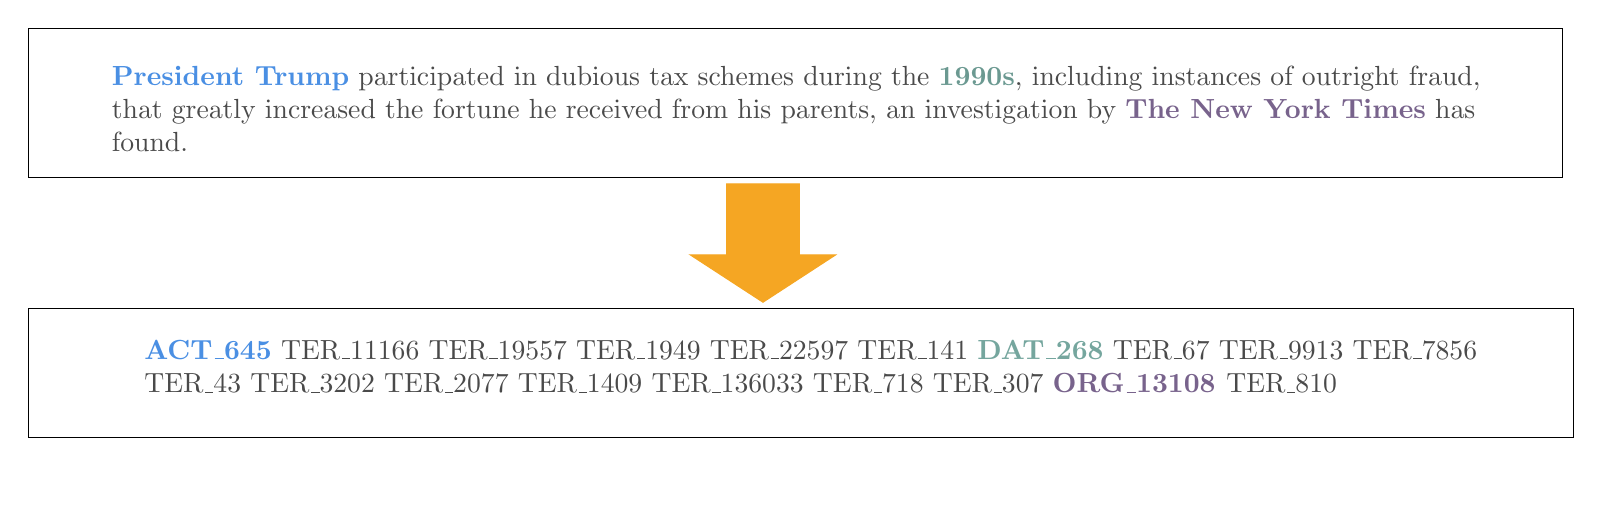
\begin{tikzpicture}[x=0.75pt,y=0.75pt,yscale=-1,xscale=1]
%uncomment if require: \path (0,377); %set diagram left start at 0, and has height of 377

%Shape: Rectangle [id:dp8906489990544584] 
\draw   (28,17) -- (767,17) -- (767,89) -- (28,89) -- cycle ;
%Shape: Rectangle [id:dp9074920271044917] 
\draw   (28,152) -- (772.5,152) -- (772.5,214) -- (28,214) -- cycle ;
%Down Arrow [id:dp1838486332286331] 
\draw  [color={rgb, 255:red, 245; green, 166; blue, 35 }  ,draw opacity=1 ][fill={rgb, 255:red, 245; green, 166; blue, 35 }  ,fill opacity=1 ] (347,126.2) -- (364.5,126.2) -- (364.5,92) -- (399.5,92) -- (399.5,126.2) -- (417,126.2) -- (382,149) -- cycle ;

% Text Node
\draw (398,80) node [scale=1,color={rgb, 255:red, 74; green, 74; blue, 74 }  ,opacity=1 ] [align=left] {\textcolor[rgb]{0.29,0.56,0.89}{\textbf{President Trump}} participated in dubious tax schemes during the \textcolor[rgb]{0.42,0.6,0.57}{\textbf{1990s}}, including instances of outright fraud, \\that greatly increased the fortune he received from his parents, an investigation by \textcolor[rgb]{0.47,0.39,0.55}{\textbf{The New York Times}} has\\found. \\\\\\};
% Text Node
\draw (405,204) node [scale=1,color={rgb, 255:red, 74; green, 74; blue, 74 }  ,opacity=1 ] [align=left] {\textbf{\textcolor[rgb]{0.29,0.56,0.89}{ACT\_645}} TER\_11166 TER\_19557 TER\_1949 TER\_22597 TER\_141 \textbf{\textcolor[rgb]{0.46,0.65,0.62}{DAT\_268}} TER\_67 TER\_9913 TER\_7856 \\TER\_43 TER\_3202 TER\_2077 TER\_1409 TER\_136033 TER\_718 TER\_307 \textbf{\textcolor[rgb]{0.47,0.39,0.55}{ORG\_13108} }TER\_810\\\\\\};


\end{tikzpicture}

}
\caption{An example of the pre-processing for annotated text. All the entity mentions are replaced with their unique identifier and the unnecessary POS-tags are removed.}
\label{fig:annotation}
\end{figure}
Named entities $N \subseteq V$ are a subset of all words in the vocabulary $N\subseteq V$ that fall into a pre-defined category.
% BR: change this to: Named entities $N \subseteq V$ are a subset of all...
In other words, terms that have a specific type are considered as named entities. Hence, the simplest way to obtain their embeddings would be to run the well-established word embedding models on the annotated text. Our contribution to these models is not the modification of the underlying method, but the input. The input of the model is no longer the raw text, but a corpus with annotated named entities. Annotation involves POS tagging, named entity recognition and disambiguation.
% BR: Would rather use 'Task of annotating them (?)' here or just say
% 'Annotation involves...'
Since word embeddings learn the representation for each token in the text, our definition of the token is changed. A token is no longer a single word separated by a space but named entity with a specific type. Any word that does not fit into any of the pre-defined types is considered as a term. Unlike the set of all words $V$, in which multiple entities can share a single ambiguous surface form, entities are presented with their unique identifiers. In our case, the identifier is the type of the word and numeric key, e.g., \emph{ACT\_17}, for an actor. As a result, compound words, such as names of people and organisations, are considered as one word. All mentions of \emph{A\_17}, which corresponds to the actor \emph{``Barack Obama''} are represented with a single identifier.
% BR: Do you mean 'identifier' rather than 'notation'?
This makes the making the text less ambiguous.
% BR: Fragment; change to 'This makes the...'
In addition, depending on the performance of the named entity recognition tool all other indirect mentions, e.g., \emph{``Mr. President''}, \emph{``President of the United States''}, are also replaced with their corresponding entity identifier.
% BR: No, the identifier is an element from that set rather than the
% whole of the set, right?($V\setminus  N$)
The same applies to different mentions of dates that result into date embeddings. Words that belong to more than one entity type, have an embedding for each type. For example, \emph{``Washington''} can either be a name of a person or a city and will have two separate embeddings for the actor and location context. The same strategy applies for terms, e.g., \emph{TER\_22}. Adding the type information in the name helps us identify and group named entities easier. It also allows us to search for a specific type. \\
Since entity annotation requires POS tagging, we used the POS tags to remove stop-words and punctuation. An example of the text after annotation and pre-processing is shown in Figure~\ref{fig:annotation}. After annotation, we use word2vec and GloVe and refer to them as $a$W2V and $a$GLV, where \emph{``a''} denotes the use of annotated text. 

\section{Node Embeddings of Co-occurrence Graphs}\label{sec:graph_based}

One motivation for incorporating the graph-based methods to enhance the performance was because of the additional information that such graphs contain. Most word embedding methods consider a fixed sized window of few words to determine if two terms are related to each other. Named entities, however, have more complex relational structures. An actor and an organization can be related even if they are mentioned several sentences apart. An example text is shown in Figure~\ref{fig:article_entities}, where possible relations between two actor entities, \emph{``Donald Trump''} and \emph{``Fred C. Trump''} are shown. If the context window is limited to a few words around the center word, then the relationship would not be detected, except for a window size of over $53$ tokens. As a result, word-based windows are unable to detect certain relationships that go beyond a sentence limit. 
% BR: Rephrase: 'the relationship would not be detected, except for
% a window size of over 53 tokens' or something like that. I believe
% you are *unable* to detect the relationship using word-based windows,
% right?
On the other hand, if we look at the sentence distance of even one sentence away, \emph{``Donald Trump''} and \emph{``Fred C. Trump''} would be considered related. This is one of the reasons behind the choice of the LOAD model as a co-occurrence network. The LOAD model applies a sentence-based window to find entity relations and a word-based window for relations among terms, and thus, captures entity-to-entity relations better than a word-based window.

\begin{figure}
\centering 
\resizebox{0.90\textwidth}{0.2\textwidth}{      
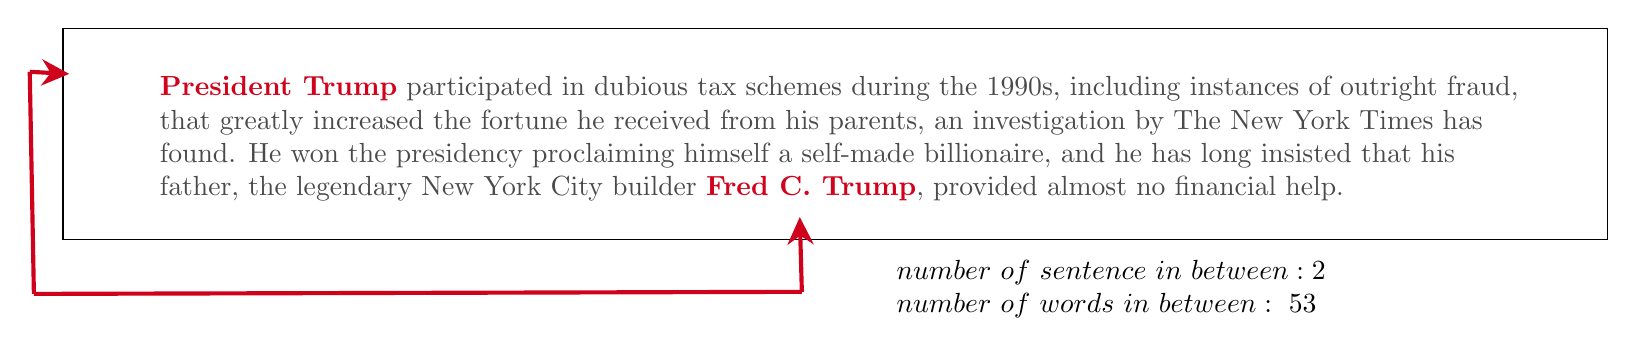
\begin{tikzpicture}[x=0.75pt,y=0.75pt,yscale=-1,xscale=1]
%uncomment if require: \path (0,300); %set diagram left start at 0, and has height of 300

%Shape: Rectangle [id:dp04377104671850285] 
\draw   (28,32) -- (772,32) -- (772,134) -- (28,134) -- cycle ;
%Straight Lines [id:da6182552655813487] 
\draw [color={rgb, 255:red, 208; green, 2; blue, 27 }  ,draw opacity=1 ][line width=1.5]    (28,53.84) -- (12,53) ;

\draw [shift={(31,54)}, rotate = 183.01] [fill={rgb, 255:red, 208; green, 2; blue, 27 }  ,fill opacity=1 ][line width=1.5]  [draw opacity=0] (13.4,-6.43) -- (0,0) -- (13.4,6.44) -- (8.9,0) -- cycle    ;
%Straight Lines [id:da6143692538402417] 
\draw [color={rgb, 255:red, 208; green, 2; blue, 27 }  ,draw opacity=1 ][line width=1.5]    (12,53) -- (14,160) ;


%Straight Lines [id:da10338493648199298] 
\draw [color={rgb, 255:red, 208; green, 2; blue, 27 }  ,draw opacity=1 ][line width=1.5]    (384,159) -- (14,160) ;


%Straight Lines [id:da054560662392693526] 
\draw [color={rgb, 255:red, 208; green, 2; blue, 27 }  ,draw opacity=1 ][line width=1.5]    (383.08,126) -- (384,159) ;

\draw [shift={(383,123)}, rotate = 88.41] [fill={rgb, 255:red, 208; green, 2; blue, 27 }  ,fill opacity=1 ][line width=1.5]  [draw opacity=0] (13.4,-6.43) -- (0,0) -- (13.4,6.44) -- (8.9,0) -- cycle    ;

% Text Node
\draw (402,108) node [scale=1,color={rgb, 255:red, 74; green, 74; blue, 74 }  ,opacity=1 ] [align=left] {\textcolor[rgb]{0.82,0.01,0.11}{\textbf{President Trump}} participated in dubious tax schemes during the 1990s, including instances of outright fraud, \\that greatly increased the fortune he received from his parents, an investigation by The New York Times has\\found. He won the presidency proclaiming himself a self-made billionaire, and he has long insisted that his \\father, the legendary New York City builder \textcolor[rgb]{0.82,0.01,0.11}{\textbf{Fred C. Trump}}, provided almost no financial help.\\\\\\};
% Text Node
\draw (533,158) node   {$ \begin{array}{l}
number\ of\ sentence\ in\ between:2\\
number\ of\ words\ in\ between:\ 53
\end{array}$};


\end{tikzpicture}

}
\caption{An example text to show the relation between two actor entities, \emph{``Donald Trump''} and \emph{``Fred C. Trump''}. If the word-based window size is applied then the relationship between the two entities is not captured, even though they are only one sentence apart.}
\label{fig:article_entities}
\end{figure}

We defined a co-occurrence graph of words in Chapter~\ref{chap:background} as a graph $G=(V,E)$, where $V$ is the set of words in the vocabulary (nodes) and $E$ is the set of edges. Furthermore, we assume that there are edge weights that encode some notion of distance between the words.
% BR: Technically, your definition does not define edge weights. So you
% could add 'Furthermore, we assume that there are edge weights that
% encode some notion of distance...'
We extract such a graph from the textual corpus with named entity annotations. As a result, we obtain a weighted heterogeneous graph $G=(N\bigcup  \overline{N},E)$ of named entities and terms, where the set $N$ contains entities of different types and $ T=\overline{N}$ denotes all the words, which are not a named entity (terms).
% BR: I do not like the choice of symbol; if you want to express the
% set-theoretic complement of $N$, use $\complement$.
For entity annotations in particular, co-occurrence graphs, which are implicitly extracted from text, such as LOAD, can serve as graph representations. By using a sentence-window for finding the relationship between entities, they can capture entity relations even sentences apart~\brackettext{\cite{DBLP:conf/sigir/SpitzG16}}. Thus, by embedding the nodes, we can obtain word embeddings for both terms and entities. We later show that this method achieves a better performance in comparison to $a$W2V and $a$GLV on the annotated text. For the node embeddings, we chose DeepWalk (DW)~\brackettext{\cite{SCHOL:website/Perozzi2014}} and VERSE (VRS)~\brackettext{\cite{SCHOL:website/Tsitsulin2018}}, explained in Chapter~\ref{chap:background}, Sections~\ref{subsec:DeepWalk} and ~\ref{subsec:VERSE} respectively.
However, since we work on weighted graphs and weights display the strength of the relationships, weighted random walks are introduced to replace the uniform random walk in the DeepWalk model.
% BR: Start the next sentence with something like 'In such a weighted
% random walk...'
In such a weighted random walk, the probability of a node visiting its neighbours is proportional to the edge weight. As a result, the probability of visiting node $j$ from vertex $i$ with edge weight $e_{i,j}$ is given in Equation~\ref{eq:edge_weight}, where $ E_{ i }$ denotes the set of all edges starting from node $v_{i}$. The stronger the relationship, the more likely a node is to be visited. So we obtain Equation~\ref{eq:edge_weight}, where $f$ is a normalization function, which we will subsequently introduce.
% BR: ...the more likely a node is to be visited
% BR: add: ...so we obtain <EQ>.
% BR: How is $f$ defined? I know it comes later, but I would rather say
% '...where $f$ is a normalization function, which we will subsequently
% introduce'

\begin{figure}
\centering 
\resizebox{0.6\textwidth}{0.6\textwidth}{      

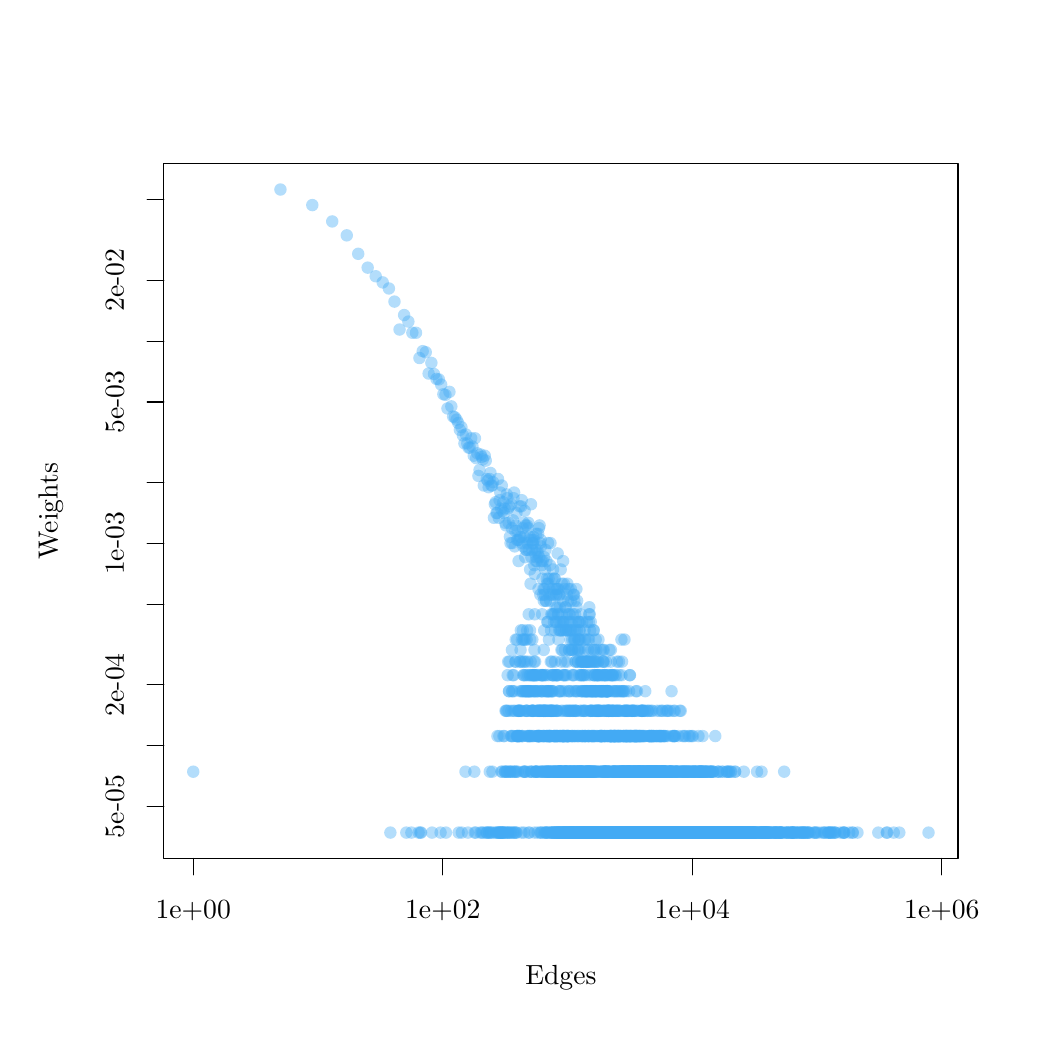
\begin{tikzpicture}[x=1pt,y=1pt]
\definecolor{fillColor}{RGB}{255,255,255}
\path[use as bounding box,fill=fillColor,fill opacity=0.00] (0,0) rectangle (361.35,361.35);
\begin{scope}
\path[clip] ( 49.20, 61.20) rectangle (336.15,312.15);
\definecolor{fillColor}{RGB}{66,170,244}

\path[fill=fillColor,fill opacity=0.40] ( 59.83, 92.50) circle (  2.25);

\path[fill=fillColor,fill opacity=0.40] ( 91.34,302.86) circle (  2.25);

\path[fill=fillColor,fill opacity=0.40] (102.85,297.24) circle (  2.25);

\path[fill=fillColor,fill opacity=0.40] (110.05,291.33) circle (  2.25);

\path[fill=fillColor,fill opacity=0.40] (115.31,286.30) circle (  2.25);

\path[fill=fillColor,fill opacity=0.40] (119.44,279.63) circle (  2.25);

\path[fill=fillColor,fill opacity=0.40] (122.86,274.63) circle (  2.25);

\path[fill=fillColor,fill opacity=0.40] (125.76,271.52) circle (  2.25);

\path[fill=fillColor,fill opacity=0.40] (128.29,269.30) circle (  2.25);

\path[fill=fillColor,fill opacity=0.40] (130.53,267.11) circle (  2.25);

\path[fill=fillColor,fill opacity=0.40] (131.06, 70.49) circle (  2.25);

\path[fill=fillColor,fill opacity=0.40] (132.54,262.37) circle (  2.25);

\path[fill=fillColor,fill opacity=0.40] (134.37,252.27) circle (  2.25);

\path[fill=fillColor,fill opacity=0.40] (136.03,257.50) circle (  2.25);

\path[fill=fillColor,fill opacity=0.40] (136.82, 70.49) circle (  2.25);

\path[fill=fillColor,fill opacity=0.40] (137.57,255.14) circle (  2.25);

\path[fill=fillColor,fill opacity=0.40] (138.65, 70.49) circle (  2.25);

\path[fill=fillColor,fill opacity=0.40] (139.00,251.11) circle (  2.25);

\path[fill=fillColor,fill opacity=0.40] (140.32,251.11) circle (  2.25);

\path[fill=fillColor,fill opacity=0.40] (141.26, 70.49) circle (  2.25);

\path[fill=fillColor,fill opacity=0.40] (141.57,241.98) circle (  2.25);

\path[fill=fillColor,fill opacity=0.40] (141.87, 70.49) circle (  2.25);

\path[fill=fillColor,fill opacity=0.40] (142.16, 70.49) circle (  2.25);

\path[fill=fillColor,fill opacity=0.40] (142.74,244.46) circle (  2.25);

\path[fill=fillColor,fill opacity=0.40] (143.84,244.06) circle (  2.25);

\path[fill=fillColor,fill opacity=0.40] (144.88,236.37) circle (  2.25);

\path[fill=fillColor,fill opacity=0.40] (145.88,240.22) circle (  2.25);

\path[fill=fillColor,fill opacity=0.40] (146.12, 70.49) circle (  2.25);

\path[fill=fillColor,fill opacity=0.40] (146.82,236.19) circle (  2.25);

\path[fill=fillColor,fill opacity=0.40] (147.72,234.43) circle (  2.25);

\path[fill=fillColor,fill opacity=0.40] (148.58,234.25) circle (  2.25);

\path[fill=fillColor,fill opacity=0.40] (149.20, 70.49) circle (  2.25);

\path[fill=fillColor,fill opacity=0.40] (149.41,232.37) circle (  2.25);

\path[fill=fillColor,fill opacity=0.40] (150.20,228.90) circle (  2.25);

\path[fill=fillColor,fill opacity=0.40] (150.96,228.68) circle (  2.25);

\path[fill=fillColor,fill opacity=0.40] (151.14, 70.49) circle (  2.25);

\path[fill=fillColor,fill opacity=0.40] (151.69,223.75) circle (  2.25);

\path[fill=fillColor,fill opacity=0.40] (152.40,229.75) circle (  2.25);

\path[fill=fillColor,fill opacity=0.40] (153.08,224.50) circle (  2.25);

\path[fill=fillColor,fill opacity=0.40] (153.74,220.83) circle (  2.25);

\path[fill=fillColor,fill opacity=0.40] (154.37,220.55) circle (  2.25);

\path[fill=fillColor,fill opacity=0.40] (154.99,219.69) circle (  2.25);

\path[fill=fillColor,fill opacity=0.40] (155.59,218.52) circle (  2.25);

\path[fill=fillColor,fill opacity=0.40] (155.73, 70.49) circle (  2.25);

\path[fill=fillColor,fill opacity=0.40] (156.17,216.03) circle (  2.25);

\path[fill=fillColor,fill opacity=0.40] (156.73,216.98) circle (  2.25);

\path[fill=fillColor,fill opacity=0.40] (156.87, 70.49) circle (  2.25);

\path[fill=fillColor,fill opacity=0.40] (157.28,214.02) circle (  2.25);

\path[fill=fillColor,fill opacity=0.40] (157.81,211.13) circle (  2.25);

\path[fill=fillColor,fill opacity=0.40] (158.20, 92.50) circle (  2.25);

\path[fill=fillColor,fill opacity=0.40] (158.33,214.36) circle (  2.25);

\path[fill=fillColor,fill opacity=0.40] (158.84,211.13) circle (  2.25);

\path[fill=fillColor,fill opacity=0.40] (159.08, 70.49) circle (  2.25);

\path[fill=fillColor,fill opacity=0.40] (159.33,209.58) circle (  2.25);

\path[fill=fillColor,fill opacity=0.40] (159.81,209.58) circle (  2.25);

\path[fill=fillColor,fill opacity=0.40] (160.28,212.97) circle (  2.25);

\path[fill=fillColor,fill opacity=0.40] (160.74,209.98) circle (  2.25);

\path[fill=fillColor,fill opacity=0.40] (161.18,206.68) circle (  2.25);

\path[fill=fillColor,fill opacity=0.40] (161.40, 92.50) circle (  2.25);

\path[fill=fillColor,fill opacity=0.40] (161.51, 70.49) circle (  2.25);

\path[fill=fillColor,fill opacity=0.40] (161.62,212.97) circle (  2.25);

\path[fill=fillColor,fill opacity=0.40] (161.94, 70.49) circle (  2.25);

\path[fill=fillColor,fill opacity=0.40] (162.05,205.80) circle (  2.25);

\path[fill=fillColor,fill opacity=0.40] (162.47,207.54) circle (  2.25);

\path[fill=fillColor,fill opacity=0.40] (162.88,199.38) circle (  2.25);

\path[fill=fillColor,fill opacity=0.40] (163.28,201.49) circle (  2.25);

\path[fill=fillColor,fill opacity=0.40] (163.58, 70.49) circle (  2.25);

\path[fill=fillColor,fill opacity=0.40] (163.67,207.11) circle (  2.25);

\path[fill=fillColor,fill opacity=0.40] (164.06,206.24) circle (  2.25);

\path[fill=fillColor,fill opacity=0.40] (164.15, 70.49) circle (  2.25);

\path[fill=fillColor,fill opacity=0.40] (164.44,205.35) circle (  2.25);

\path[fill=fillColor,fill opacity=0.40] (164.62, 70.49) circle (  2.25);

\path[fill=fillColor,fill opacity=0.40] (164.81,195.91) circle (  2.25);

\path[fill=fillColor,fill opacity=0.40] (165.17,206.68) circle (  2.25);

\path[fill=fillColor,fill opacity=0.40] (165.53,204.89) circle (  2.25);

\path[fill=fillColor,fill opacity=0.40] (165.62, 70.49) circle (  2.25);

\path[fill=fillColor,fill opacity=0.40] (165.88,198.26) circle (  2.25);

\path[fill=fillColor,fill opacity=0.40] (165.97, 70.49) circle (  2.25);

\path[fill=fillColor,fill opacity=0.40] (166.05, 70.49) circle (  2.25);

\path[fill=fillColor,fill opacity=0.40] (166.23,197.69) circle (  2.25);

\path[fill=fillColor,fill opacity=0.40] (166.57,195.29) circle (  2.25);

\path[fill=fillColor,fill opacity=0.40] (166.65, 70.49) circle (  2.25);

\path[fill=fillColor,fill opacity=0.40] (166.73, 70.49) circle (  2.25);

\path[fill=fillColor,fill opacity=0.40] (166.90,198.26) circle (  2.25);

\path[fill=fillColor,fill opacity=0.40] (166.98, 92.50) circle (  2.25);

\path[fill=fillColor,fill opacity=0.40] (167.23,200.45) circle (  2.25);

\path[fill=fillColor,fill opacity=0.40] (167.31, 70.49) circle (  2.25);

\path[fill=fillColor,fill opacity=0.40] (167.47, 70.49) circle (  2.25);

\path[fill=fillColor,fill opacity=0.40] (167.55,195.91) circle (  2.25);

\path[fill=fillColor,fill opacity=0.40] (167.87,195.91) circle (  2.25);

\path[fill=fillColor,fill opacity=0.40] (167.94, 92.50) circle (  2.25);

\path[fill=fillColor,fill opacity=0.40] (168.18,197.11) circle (  2.25);

\path[fill=fillColor,fill opacity=0.40] (168.26, 70.49) circle (  2.25);

\path[fill=fillColor,fill opacity=0.40] (168.49,184.24) circle (  2.25);

\path[fill=fillColor,fill opacity=0.40] (168.79,189.13) circle (  2.25);

\path[fill=fillColor,fill opacity=0.40] (169.09,189.88) circle (  2.25);

\path[fill=fillColor,fill opacity=0.40] (169.23, 70.49) circle (  2.25);

\path[fill=fillColor,fill opacity=0.40] (169.31, 70.49) circle (  2.25);

\path[fill=fillColor,fill opacity=0.40] (169.38,185.96) circle (  2.25);

\path[fill=fillColor,fill opacity=0.40] (169.67,185.96) circle (  2.25);

\path[fill=fillColor,fill opacity=0.40] (169.74,105.37) circle (  2.25);

\path[fill=fillColor,fill opacity=0.40] (169.81, 70.49) circle (  2.25);

\path[fill=fillColor,fill opacity=0.40] (169.95,198.26) circle (  2.25);

\path[fill=fillColor,fill opacity=0.40] (170.16, 70.49) circle (  2.25);

\path[fill=fillColor,fill opacity=0.40] (170.23,184.24) circle (  2.25);

\path[fill=fillColor,fill opacity=0.40] (170.30, 70.49) circle (  2.25);

\path[fill=fillColor,fill opacity=0.40] (170.37, 70.49) circle (  2.25);

\path[fill=fillColor,fill opacity=0.40] (170.44,105.37) circle (  2.25);

\path[fill=fillColor,fill opacity=0.40] (170.51,190.61) circle (  2.25);

\path[fill=fillColor,fill opacity=0.40] (170.58, 70.49) circle (  2.25);

\path[fill=fillColor,fill opacity=0.40] (170.72, 70.49) circle (  2.25);

\path[fill=fillColor,fill opacity=0.40] (170.78,193.37) circle (  2.25);

\path[fill=fillColor,fill opacity=0.40] (170.85, 70.49) circle (  2.25);

\path[fill=fillColor,fill opacity=0.40] (171.05,187.58) circle (  2.25);

\path[fill=fillColor,fill opacity=0.40] (171.19, 92.50) circle (  2.25);

\path[fill=fillColor,fill opacity=0.40] (171.25, 70.49) circle (  2.25);

\path[fill=fillColor,fill opacity=0.40] (171.32,195.91) circle (  2.25);

\path[fill=fillColor,fill opacity=0.40] (171.38, 70.49) circle (  2.25);

\path[fill=fillColor,fill opacity=0.40] (171.45, 92.50) circle (  2.25);

\path[fill=fillColor,fill opacity=0.40] (171.51, 70.49) circle (  2.25);

\path[fill=fillColor,fill opacity=0.40] (171.58,186.78) circle (  2.25);

\path[fill=fillColor,fill opacity=0.40] (171.64, 70.49) circle (  2.25);

\path[fill=fillColor,fill opacity=0.40] (171.71, 70.49) circle (  2.25);

\path[fill=fillColor,fill opacity=0.40] (171.77, 70.49) circle (  2.25);

\path[fill=fillColor,fill opacity=0.40] (171.84,189.88) circle (  2.25);

\path[fill=fillColor,fill opacity=0.40] (171.90,105.37) circle (  2.25);

\path[fill=fillColor,fill opacity=0.40] (172.09,185.96) circle (  2.25);

\path[fill=fillColor,fill opacity=0.40] (172.16, 70.49) circle (  2.25);

\path[fill=fillColor,fill opacity=0.40] (172.28,105.37) circle (  2.25);

\path[fill=fillColor,fill opacity=0.40] (172.35,187.58) circle (  2.25);

\path[fill=fillColor,fill opacity=0.40] (172.41, 92.50) circle (  2.25);

\path[fill=fillColor,fill opacity=0.40] (172.47, 92.50) circle (  2.25);

\path[fill=fillColor,fill opacity=0.40] (172.53, 70.49) circle (  2.25);

\path[fill=fillColor,fill opacity=0.40] (172.59,182.42) circle (  2.25);

\path[fill=fillColor,fill opacity=0.40] (172.66,114.50) circle (  2.25);

\path[fill=fillColor,fill opacity=0.40] (172.72, 92.50) circle (  2.25);

\path[fill=fillColor,fill opacity=0.40] (172.78, 70.49) circle (  2.25);

\path[fill=fillColor,fill opacity=0.40] (172.84,181.48) circle (  2.25);

\path[fill=fillColor,fill opacity=0.40] (172.90,114.50) circle (  2.25);

\path[fill=fillColor,fill opacity=0.40] (173.02, 92.50) circle (  2.25);

\path[fill=fillColor,fill opacity=0.40] (173.08,192.70) circle (  2.25);

\path[fill=fillColor,fill opacity=0.40] (173.14,114.50) circle (  2.25);

\path[fill=fillColor,fill opacity=0.40] (173.26, 92.50) circle (  2.25);

\path[fill=fillColor,fill opacity=0.40] (173.32,191.32) circle (  2.25);

\path[fill=fillColor,fill opacity=0.40] (173.38, 70.49) circle (  2.25);

\path[fill=fillColor,fill opacity=0.40] (173.44,127.37) circle (  2.25);

\path[fill=fillColor,fill opacity=0.40] (173.50, 70.49) circle (  2.25);

\path[fill=fillColor,fill opacity=0.40] (173.56,187.58) circle (  2.25);

\path[fill=fillColor,fill opacity=0.40] (173.62,132.26) circle (  2.25);

\path[fill=fillColor,fill opacity=0.40] (173.68, 70.49) circle (  2.25);

\path[fill=fillColor,fill opacity=0.40] (173.73,114.50) circle (  2.25);

\path[fill=fillColor,fill opacity=0.40] (173.79,182.42) circle (  2.25);

\path[fill=fillColor,fill opacity=0.40] (173.85, 92.50) circle (  2.25);

\path[fill=fillColor,fill opacity=0.40] (173.91,121.58) circle (  2.25);

\path[fill=fillColor,fill opacity=0.40] (173.97,121.58) circle (  2.25);

\path[fill=fillColor,fill opacity=0.40] (174.02,188.37) circle (  2.25);

\path[fill=fillColor,fill opacity=0.40] (174.08,132.26) circle (  2.25);

\path[fill=fillColor,fill opacity=0.40] (174.14, 70.49) circle (  2.25);

\path[fill=fillColor,fill opacity=0.40] (174.25,177.38) circle (  2.25);

\path[fill=fillColor,fill opacity=0.40] (174.31, 92.50) circle (  2.25);

\path[fill=fillColor,fill opacity=0.40] (174.42, 92.50) circle (  2.25);

\path[fill=fillColor,fill opacity=0.40] (174.48,175.11) circle (  2.25);

\path[fill=fillColor,fill opacity=0.40] (174.53, 70.49) circle (  2.25);

\path[fill=fillColor,fill opacity=0.40] (174.59, 92.50) circle (  2.25);

\path[fill=fillColor,fill opacity=0.40] (174.64,105.37) circle (  2.25);

\path[fill=fillColor,fill opacity=0.40] (174.70,189.13) circle (  2.25);

\path[fill=fillColor,fill opacity=0.40] (174.76,114.50) circle (  2.25);

\path[fill=fillColor,fill opacity=0.40] (174.81,105.37) circle (  2.25);

\path[fill=fillColor,fill opacity=0.40] (174.87, 70.49) circle (  2.25);

\path[fill=fillColor,fill opacity=0.40] (174.92,180.50) circle (  2.25);

\path[fill=fillColor,fill opacity=0.40] (174.98,136.50) circle (  2.25);

\path[fill=fillColor,fill opacity=0.40] (175.03,121.58) circle (  2.25);

\path[fill=fillColor,fill opacity=0.40] (175.08,105.37) circle (  2.25);

\path[fill=fillColor,fill opacity=0.40] (175.14,175.11) circle (  2.25);

\path[fill=fillColor,fill opacity=0.40] (175.19,121.58) circle (  2.25);

\path[fill=fillColor,fill opacity=0.40] (175.25,127.37) circle (  2.25);

\path[fill=fillColor,fill opacity=0.40] (175.30, 92.50) circle (  2.25);

\path[fill=fillColor,fill opacity=0.40] (175.35,183.34) circle (  2.25);

\path[fill=fillColor,fill opacity=0.40] (175.41, 70.49) circle (  2.25);

\path[fill=fillColor,fill opacity=0.40] (175.46,105.37) circle (  2.25);

\path[fill=fillColor,fill opacity=0.40] (175.52,114.50) circle (  2.25);

\path[fill=fillColor,fill opacity=0.40] (175.57,191.32) circle (  2.25);

\path[fill=fillColor,fill opacity=0.40] (175.62,127.37) circle (  2.25);

\path[fill=fillColor,fill opacity=0.40] (175.73, 70.49) circle (  2.25);

\path[fill=fillColor,fill opacity=0.40] (175.78,193.37) circle (  2.25);

\path[fill=fillColor,fill opacity=0.40] (175.83,121.58) circle (  2.25);

\path[fill=fillColor,fill opacity=0.40] (175.88, 92.50) circle (  2.25);

\path[fill=fillColor,fill opacity=0.40] (175.94, 92.50) circle (  2.25);

\path[fill=fillColor,fill opacity=0.40] (175.99,173.91) circle (  2.25);

\path[fill=fillColor,fill opacity=0.40] (176.04,114.50) circle (  2.25);

\path[fill=fillColor,fill opacity=0.40] (176.09, 70.49) circle (  2.25);

\path[fill=fillColor,fill opacity=0.40] (176.20,179.49) circle (  2.25);

\path[fill=fillColor,fill opacity=0.40] (176.25,132.26) circle (  2.25);

\path[fill=fillColor,fill opacity=0.40] (176.30,132.26) circle (  2.25);

\path[fill=fillColor,fill opacity=0.40] (176.35,140.24) circle (  2.25);

\path[fill=fillColor,fill opacity=0.40] (176.40,181.48) circle (  2.25);

\path[fill=fillColor,fill opacity=0.40] (176.45, 70.49) circle (  2.25);

\path[fill=fillColor,fill opacity=0.40] (176.50, 92.50) circle (  2.25);

\path[fill=fillColor,fill opacity=0.40] (176.55, 92.50) circle (  2.25);

\path[fill=fillColor,fill opacity=0.40] (176.60,185.96) circle (  2.25);

\path[fill=fillColor,fill opacity=0.40] (176.65, 70.49) circle (  2.25);

\path[fill=fillColor,fill opacity=0.40] (176.70,105.37) circle (  2.25);

\path[fill=fillColor,fill opacity=0.40] (176.75,105.37) circle (  2.25);

\path[fill=fillColor,fill opacity=0.40] (176.80,176.26) circle (  2.25);

\path[fill=fillColor,fill opacity=0.40] (176.85,140.24) circle (  2.25);

\path[fill=fillColor,fill opacity=0.40] (176.90,105.37) circle (  2.25);

\path[fill=fillColor,fill opacity=0.40] (176.95,105.37) circle (  2.25);

\path[fill=fillColor,fill opacity=0.40] (177.00,179.49) circle (  2.25);

\path[fill=fillColor,fill opacity=0.40] (177.05,114.50) circle (  2.25);

\path[fill=fillColor,fill opacity=0.40] (177.10,105.37) circle (  2.25);

\path[fill=fillColor,fill opacity=0.40] (177.15, 92.50) circle (  2.25);

\path[fill=fillColor,fill opacity=0.40] (177.20,176.26) circle (  2.25);

\path[fill=fillColor,fill opacity=0.40] (177.25,105.37) circle (  2.25);

\path[fill=fillColor,fill opacity=0.40] (177.29,114.50) circle (  2.25);

\path[fill=fillColor,fill opacity=0.40] (177.34,114.50) circle (  2.25);

\path[fill=fillColor,fill opacity=0.40] (177.39,168.61) circle (  2.25);

\path[fill=fillColor,fill opacity=0.40] (177.44,114.50) circle (  2.25);

\path[fill=fillColor,fill opacity=0.40] (177.49,105.37) circle (  2.25);

\path[fill=fillColor,fill opacity=0.40] (177.54,114.50) circle (  2.25);

\path[fill=fillColor,fill opacity=0.40] (177.58,176.26) circle (  2.25);

\path[fill=fillColor,fill opacity=0.40] (177.63,105.37) circle (  2.25);

\path[fill=fillColor,fill opacity=0.40] (177.68,105.37) circle (  2.25);

\path[fill=fillColor,fill opacity=0.40] (177.73,114.50) circle (  2.25);

\path[fill=fillColor,fill opacity=0.40] (177.77,188.37) circle (  2.25);

\path[fill=fillColor,fill opacity=0.40] (177.82,132.26) circle (  2.25);

\path[fill=fillColor,fill opacity=0.40] (177.87,105.37) circle (  2.25);

\path[fill=fillColor,fill opacity=0.40] (177.92,114.50) circle (  2.25);

\path[fill=fillColor,fill opacity=0.40] (177.96,177.38) circle (  2.25);

\path[fill=fillColor,fill opacity=0.40] (178.01,121.58) circle (  2.25);

\path[fill=fillColor,fill opacity=0.40] (178.06,132.26) circle (  2.25);

\path[fill=fillColor,fill opacity=0.40] (178.10,136.50) circle (  2.25);

\path[fill=fillColor,fill opacity=0.40] (178.15,177.38) circle (  2.25);

\path[fill=fillColor,fill opacity=0.40] (178.20,143.58) circle (  2.25);

\path[fill=fillColor,fill opacity=0.40] (178.24,114.50) circle (  2.25);

\path[fill=fillColor,fill opacity=0.40] (178.34,188.37) circle (  2.25);

\path[fill=fillColor,fill opacity=0.40] (178.38,114.50) circle (  2.25);

\path[fill=fillColor,fill opacity=0.40] (178.43, 70.49) circle (  2.25);

\path[fill=fillColor,fill opacity=0.40] (178.47,121.58) circle (  2.25);

\path[fill=fillColor,fill opacity=0.40] (178.52,190.61) circle (  2.25);

\path[fill=fillColor,fill opacity=0.40] (178.56,140.24) circle (  2.25);

\path[fill=fillColor,fill opacity=0.40] (178.61,105.37) circle (  2.25);

\path[fill=fillColor,fill opacity=0.40] (178.65,105.37) circle (  2.25);

\path[fill=fillColor,fill opacity=0.40] (178.70,175.11) circle (  2.25);

\path[fill=fillColor,fill opacity=0.40] (178.75,132.26) circle (  2.25);

\path[fill=fillColor,fill opacity=0.40] (178.79,121.58) circle (  2.25);

\path[fill=fillColor,fill opacity=0.40] (178.84,105.37) circle (  2.25);

\path[fill=fillColor,fill opacity=0.40] (178.88,180.50) circle (  2.25);

\path[fill=fillColor,fill opacity=0.40] (178.93,143.58) circle (  2.25);

\path[fill=fillColor,fill opacity=0.40] (178.97,121.58) circle (  2.25);

\path[fill=fillColor,fill opacity=0.40] (179.01, 92.50) circle (  2.25);

\path[fill=fillColor,fill opacity=0.40] (179.06,173.91) circle (  2.25);

\path[fill=fillColor,fill opacity=0.40] (179.10,140.24) circle (  2.25);

\path[fill=fillColor,fill opacity=0.40] (179.15,127.37) circle (  2.25);

\path[fill=fillColor,fill opacity=0.40] (179.19,127.37) circle (  2.25);

\path[fill=fillColor,fill opacity=0.40] (179.24,182.42) circle (  2.25);

\path[fill=fillColor,fill opacity=0.40] (179.28,140.24) circle (  2.25);

\path[fill=fillColor,fill opacity=0.40] (179.32,132.26) circle (  2.25);

\path[fill=fillColor,fill opacity=0.40] (179.37, 70.49) circle (  2.25);

\path[fill=fillColor,fill opacity=0.40] (179.41,177.38) circle (  2.25);

\path[fill=fillColor,fill opacity=0.40] (179.45, 92.50) circle (  2.25);

\path[fill=fillColor,fill opacity=0.40] (179.50,121.58) circle (  2.25);

\path[fill=fillColor,fill opacity=0.40] (179.54, 92.50) circle (  2.25);

\path[fill=fillColor,fill opacity=0.40] (179.58,186.78) circle (  2.25);

\path[fill=fillColor,fill opacity=0.40] (179.63,127.37) circle (  2.25);

\path[fill=fillColor,fill opacity=0.40] (179.67,132.26) circle (  2.25);

\path[fill=fillColor,fill opacity=0.40] (179.71, 92.50) circle (  2.25);

\path[fill=fillColor,fill opacity=0.40] (179.76,170.02) circle (  2.25);

\path[fill=fillColor,fill opacity=0.40] (179.80,140.24) circle (  2.25);

\path[fill=fillColor,fill opacity=0.40] (179.84,121.58) circle (  2.25);

\path[fill=fillColor,fill opacity=0.40] (179.88, 92.50) circle (  2.25);

\path[fill=fillColor,fill opacity=0.40] (179.93,181.48) circle (  2.25);

\path[fill=fillColor,fill opacity=0.40] (179.97,121.58) circle (  2.25);

\path[fill=fillColor,fill opacity=0.40] (180.01,114.50) circle (  2.25);

\path[fill=fillColor,fill opacity=0.40] (180.05,121.58) circle (  2.25);

\path[fill=fillColor,fill opacity=0.40] (180.10,172.66) circle (  2.25);

\path[fill=fillColor,fill opacity=0.40] (180.14,114.50) circle (  2.25);

\path[fill=fillColor,fill opacity=0.40] (180.18,121.58) circle (  2.25);

\path[fill=fillColor,fill opacity=0.40] (180.22,127.37) circle (  2.25);

\path[fill=fillColor,fill opacity=0.40] (180.26,172.66) circle (  2.25);

\path[fill=fillColor,fill opacity=0.40] (180.31,140.24) circle (  2.25);

\path[fill=fillColor,fill opacity=0.40] (180.35,114.50) circle (  2.25);

\path[fill=fillColor,fill opacity=0.40] (180.39,114.50) circle (  2.25);

\path[fill=fillColor,fill opacity=0.40] (180.43,181.48) circle (  2.25);

\path[fill=fillColor,fill opacity=0.40] (180.47,143.58) circle (  2.25);

\path[fill=fillColor,fill opacity=0.40] (180.51,114.50) circle (  2.25);

\path[fill=fillColor,fill opacity=0.40] (180.55,132.26) circle (  2.25);

\path[fill=fillColor,fill opacity=0.40] (180.60,175.11) circle (  2.25);

\path[fill=fillColor,fill opacity=0.40] (180.64,105.37) circle (  2.25);

\path[fill=fillColor,fill opacity=0.40] (180.68,105.37) circle (  2.25);

\path[fill=fillColor,fill opacity=0.40] (180.72,121.58) circle (  2.25);

\path[fill=fillColor,fill opacity=0.40] (180.76,180.50) circle (  2.25);

\path[fill=fillColor,fill opacity=0.40] (180.80,121.58) circle (  2.25);

\path[fill=fillColor,fill opacity=0.40] (180.84,105.37) circle (  2.25);

\path[fill=fillColor,fill opacity=0.40] (180.88,127.37) circle (  2.25);

\path[fill=fillColor,fill opacity=0.40] (180.92,182.42) circle (  2.25);

\path[fill=fillColor,fill opacity=0.40] (180.96, 70.49) circle (  2.25);

\path[fill=fillColor,fill opacity=0.40] (181.00,121.58) circle (  2.25);

\path[fill=fillColor,fill opacity=0.40] (181.04,149.37) circle (  2.25);

\path[fill=fillColor,fill opacity=0.40] (181.08,172.66) circle (  2.25);

\path[fill=fillColor,fill opacity=0.40] (181.12,121.58) circle (  2.25);

\path[fill=fillColor,fill opacity=0.40] (181.16, 92.50) circle (  2.25);

\path[fill=fillColor,fill opacity=0.40] (181.20,105.37) circle (  2.25);

\path[fill=fillColor,fill opacity=0.40] (181.24,176.26) circle (  2.25);

\path[fill=fillColor,fill opacity=0.40] (181.28,121.58) circle (  2.25);

\path[fill=fillColor,fill opacity=0.40] (181.32, 70.49) circle (  2.25);

\path[fill=fillColor,fill opacity=0.40] (181.36,105.37) circle (  2.25);

\path[fill=fillColor,fill opacity=0.40] (181.40,177.38) circle (  2.25);

\path[fill=fillColor,fill opacity=0.40] (181.44,127.37) circle (  2.25);

\path[fill=fillColor,fill opacity=0.40] (181.48,105.37) circle (  2.25);

\path[fill=fillColor,fill opacity=0.40] (181.52,143.58) circle (  2.25);

\path[fill=fillColor,fill opacity=0.40] (181.56,165.58) circle (  2.25);

\path[fill=fillColor,fill opacity=0.40] (181.60,140.24) circle (  2.25);

\path[fill=fillColor,fill opacity=0.40] (181.63,121.58) circle (  2.25);

\path[fill=fillColor,fill opacity=0.40] (181.67,127.37) circle (  2.25);

\path[fill=fillColor,fill opacity=0.40] (181.71,160.42) circle (  2.25);

\path[fill=fillColor,fill opacity=0.40] (181.75,132.26) circle (  2.25);

\path[fill=fillColor,fill opacity=0.40] (181.79,105.37) circle (  2.25);

\path[fill=fillColor,fill opacity=0.40] (181.83,121.58) circle (  2.25);

\path[fill=fillColor,fill opacity=0.40] (181.87,189.13) circle (  2.25);

\path[fill=fillColor,fill opacity=0.40] (181.91,114.50) circle (  2.25);

\path[fill=fillColor,fill opacity=0.40] (181.94, 92.50) circle (  2.25);

\path[fill=fillColor,fill opacity=0.40] (181.98, 92.50) circle (  2.25);

\path[fill=fillColor,fill opacity=0.40] (182.02,170.02) circle (  2.25);

\path[fill=fillColor,fill opacity=0.40] (182.06,105.37) circle (  2.25);

\path[fill=fillColor,fill opacity=0.40] (182.10,121.58) circle (  2.25);

\path[fill=fillColor,fill opacity=0.40] (182.13,114.50) circle (  2.25);

\path[fill=fillColor,fill opacity=0.40] (182.17,176.26) circle (  2.25);

\path[fill=fillColor,fill opacity=0.40] (182.21, 92.50) circle (  2.25);

\path[fill=fillColor,fill opacity=0.40] (182.25,127.37) circle (  2.25);

\path[fill=fillColor,fill opacity=0.40] (182.29,114.50) circle (  2.25);

\path[fill=fillColor,fill opacity=0.40] (182.32,172.66) circle (  2.25);

\path[fill=fillColor,fill opacity=0.40] (182.36,140.24) circle (  2.25);

\path[fill=fillColor,fill opacity=0.40] (182.40,127.37) circle (  2.25);

\path[fill=fillColor,fill opacity=0.40] (182.44,114.50) circle (  2.25);

\path[fill=fillColor,fill opacity=0.40] (182.47,175.11) circle (  2.25);

\path[fill=fillColor,fill opacity=0.40] (182.51,105.37) circle (  2.25);

\path[fill=fillColor,fill opacity=0.40] (182.55,114.50) circle (  2.25);

\path[fill=fillColor,fill opacity=0.40] (182.58,114.50) circle (  2.25);

\path[fill=fillColor,fill opacity=0.40] (182.62,175.11) circle (  2.25);

\path[fill=fillColor,fill opacity=0.40] (182.66,127.37) circle (  2.25);

\path[fill=fillColor,fill opacity=0.40] (182.70,114.50) circle (  2.25);

\path[fill=fillColor,fill opacity=0.40] (182.73,121.58) circle (  2.25);

\path[fill=fillColor,fill opacity=0.40] (182.77,177.38) circle (  2.25);

\path[fill=fillColor,fill opacity=0.40] (182.81,114.50) circle (  2.25);

\path[fill=fillColor,fill opacity=0.40] (182.84,127.37) circle (  2.25);

\path[fill=fillColor,fill opacity=0.40] (182.88,105.37) circle (  2.25);

\path[fill=fillColor,fill opacity=0.40] (182.92,176.26) circle (  2.25);

\path[fill=fillColor,fill opacity=0.40] (182.95,121.58) circle (  2.25);

\path[fill=fillColor,fill opacity=0.40] (182.99,132.26) circle (  2.25);

\path[fill=fillColor,fill opacity=0.40] (183.02,127.37) circle (  2.25);

\path[fill=fillColor,fill opacity=0.40] (183.06,167.13) circle (  2.25);

\path[fill=fillColor,fill opacity=0.40] (183.10,127.37) circle (  2.25);

\path[fill=fillColor,fill opacity=0.40] (183.13,136.50) circle (  2.25);

\path[fill=fillColor,fill opacity=0.40] (183.17, 70.49) circle (  2.25);

\path[fill=fillColor,fill opacity=0.40] (183.20,163.95) circle (  2.25);

\path[fill=fillColor,fill opacity=0.40] (183.24,149.37) circle (  2.25);

\path[fill=fillColor,fill opacity=0.40] (183.28,127.37) circle (  2.25);

\path[fill=fillColor,fill opacity=0.40] (183.35,171.37) circle (  2.25);

\path[fill=fillColor,fill opacity=0.40] (183.38,132.26) circle (  2.25);

\path[fill=fillColor,fill opacity=0.40] (183.42,121.58) circle (  2.25);

\path[fill=fillColor,fill opacity=0.40] (183.45,121.58) circle (  2.25);

\path[fill=fillColor,fill opacity=0.40] (183.49,172.66) circle (  2.25);

\path[fill=fillColor,fill opacity=0.40] (183.53, 92.50) circle (  2.25);

\path[fill=fillColor,fill opacity=0.40] (183.56, 92.50) circle (  2.25);

\path[fill=fillColor,fill opacity=0.40] (183.60, 92.50) circle (  2.25);

\path[fill=fillColor,fill opacity=0.40] (183.63,168.61) circle (  2.25);

\path[fill=fillColor,fill opacity=0.40] (183.67,127.37) circle (  2.25);

\path[fill=fillColor,fill opacity=0.40] (183.70, 92.50) circle (  2.25);

\path[fill=fillColor,fill opacity=0.40] (183.74, 92.50) circle (  2.25);

\path[fill=fillColor,fill opacity=0.40] (183.77,178.45) circle (  2.25);

\path[fill=fillColor,fill opacity=0.40] (183.81,127.37) circle (  2.25);

\path[fill=fillColor,fill opacity=0.40] (183.84,121.58) circle (  2.25);

\path[fill=fillColor,fill opacity=0.40] (183.88, 92.50) circle (  2.25);

\path[fill=fillColor,fill opacity=0.40] (183.91,170.02) circle (  2.25);

\path[fill=fillColor,fill opacity=0.40] (183.95,105.37) circle (  2.25);

\path[fill=fillColor,fill opacity=0.40] (183.98,105.37) circle (  2.25);

\path[fill=fillColor,fill opacity=0.40] (184.01,114.50) circle (  2.25);

\path[fill=fillColor,fill opacity=0.40] (184.05,168.61) circle (  2.25);

\path[fill=fillColor,fill opacity=0.40] (184.08,114.50) circle (  2.25);

\path[fill=fillColor,fill opacity=0.40] (184.12,114.50) circle (  2.25);

\path[fill=fillColor,fill opacity=0.40] (184.15,105.37) circle (  2.25);

\path[fill=fillColor,fill opacity=0.40] (184.19,172.66) circle (  2.25);

\path[fill=fillColor,fill opacity=0.40] (184.22,127.37) circle (  2.25);

\path[fill=fillColor,fill opacity=0.40] (184.25, 70.49) circle (  2.25);

\path[fill=fillColor,fill opacity=0.40] (184.29,121.58) circle (  2.25);

\path[fill=fillColor,fill opacity=0.40] (184.32,171.37) circle (  2.25);

\path[fill=fillColor,fill opacity=0.40] (184.36,105.37) circle (  2.25);

\path[fill=fillColor,fill opacity=0.40] (184.39, 92.50) circle (  2.25);

\path[fill=fillColor,fill opacity=0.40] (184.42,121.58) circle (  2.25);

\path[fill=fillColor,fill opacity=0.40] (184.46,178.45) circle (  2.25);

\path[fill=fillColor,fill opacity=0.40] (184.49,114.50) circle (  2.25);

\path[fill=fillColor,fill opacity=0.40] (184.52,105.37) circle (  2.25);

\path[fill=fillColor,fill opacity=0.40] (184.56,105.37) circle (  2.25);

\path[fill=fillColor,fill opacity=0.40] (184.59,158.50) circle (  2.25);

\path[fill=fillColor,fill opacity=0.40] (184.63,105.37) circle (  2.25);

\path[fill=fillColor,fill opacity=0.40] (184.66,105.37) circle (  2.25);

\path[fill=fillColor,fill opacity=0.40] (184.69,114.50) circle (  2.25);

\path[fill=fillColor,fill opacity=0.40] (184.73,180.50) circle (  2.25);

\path[fill=fillColor,fill opacity=0.40] (184.76,114.50) circle (  2.25);

\path[fill=fillColor,fill opacity=0.40] (184.79,105.37) circle (  2.25);

\path[fill=fillColor,fill opacity=0.40] (184.86,170.02) circle (  2.25);

\path[fill=fillColor,fill opacity=0.40] (184.89,105.37) circle (  2.25);

\path[fill=fillColor,fill opacity=0.40] (184.96,105.37) circle (  2.25);

\path[fill=fillColor,fill opacity=0.40] (184.99,181.48) circle (  2.25);

\path[fill=fillColor,fill opacity=0.40] (185.02,114.50) circle (  2.25);

\path[fill=fillColor,fill opacity=0.40] (185.05,114.50) circle (  2.25);

\path[fill=fillColor,fill opacity=0.40] (185.09, 92.50) circle (  2.25);

\path[fill=fillColor,fill opacity=0.40] (185.12,175.11) circle (  2.25);

\path[fill=fillColor,fill opacity=0.40] (185.15,114.50) circle (  2.25);

\path[fill=fillColor,fill opacity=0.40] (185.19,105.37) circle (  2.25);

\path[fill=fillColor,fill opacity=0.40] (185.25,156.45) circle (  2.25);

\path[fill=fillColor,fill opacity=0.40] (185.28,114.50) circle (  2.25);

\path[fill=fillColor,fill opacity=0.40] (185.31, 70.49) circle (  2.25);

\path[fill=fillColor,fill opacity=0.40] (185.35, 70.49) circle (  2.25);

\path[fill=fillColor,fill opacity=0.40] (185.38,176.26) circle (  2.25);

\path[fill=fillColor,fill opacity=0.40] (185.41,127.37) circle (  2.25);

\path[fill=fillColor,fill opacity=0.40] (185.44, 92.50) circle (  2.25);

\path[fill=fillColor,fill opacity=0.40] (185.48,114.50) circle (  2.25);

\path[fill=fillColor,fill opacity=0.40] (185.51,173.91) circle (  2.25);

\path[fill=fillColor,fill opacity=0.40] (185.54,127.37) circle (  2.25);

\path[fill=fillColor,fill opacity=0.40] (185.57,114.50) circle (  2.25);

\path[fill=fillColor,fill opacity=0.40] (185.60,121.58) circle (  2.25);

\path[fill=fillColor,fill opacity=0.40] (185.63,168.61) circle (  2.25);

\path[fill=fillColor,fill opacity=0.40] (185.67,121.58) circle (  2.25);

\path[fill=fillColor,fill opacity=0.40] (185.70,121.58) circle (  2.25);

\path[fill=fillColor,fill opacity=0.40] (185.73,105.37) circle (  2.25);

\path[fill=fillColor,fill opacity=0.40] (185.76,167.13) circle (  2.25);

\path[fill=fillColor,fill opacity=0.40] (185.79, 92.50) circle (  2.25);

\path[fill=fillColor,fill opacity=0.40] (185.82,127.37) circle (  2.25);

\path[fill=fillColor,fill opacity=0.40] (185.86, 70.49) circle (  2.25);

\path[fill=fillColor,fill opacity=0.40] (185.89,149.37) circle (  2.25);

\path[fill=fillColor,fill opacity=0.40] (185.92,114.50) circle (  2.25);

\path[fill=fillColor,fill opacity=0.40] (185.95, 92.50) circle (  2.25);

\path[fill=fillColor,fill opacity=0.40] (185.98, 92.50) circle (  2.25);

\path[fill=fillColor,fill opacity=0.40] (186.01,162.24) circle (  2.25);

\path[fill=fillColor,fill opacity=0.40] (186.04,127.37) circle (  2.25);

\path[fill=fillColor,fill opacity=0.40] (186.07,105.37) circle (  2.25);

\path[fill=fillColor,fill opacity=0.40] (186.10,121.58) circle (  2.25);

\path[fill=fillColor,fill opacity=0.40] (186.14,168.61) circle (  2.25);

\path[fill=fillColor,fill opacity=0.40] (186.17,127.37) circle (  2.25);

\path[fill=fillColor,fill opacity=0.40] (186.20,127.37) circle (  2.25);

\path[fill=fillColor,fill opacity=0.40] (186.23,105.37) circle (  2.25);

\path[fill=fillColor,fill opacity=0.40] (186.26,156.45) circle (  2.25);

\path[fill=fillColor,fill opacity=0.40] (186.29,114.50) circle (  2.25);

\path[fill=fillColor,fill opacity=0.40] (186.32,114.50) circle (  2.25);

\path[fill=fillColor,fill opacity=0.40] (186.35,114.50) circle (  2.25);

\path[fill=fillColor,fill opacity=0.40] (186.38,158.50) circle (  2.25);

\path[fill=fillColor,fill opacity=0.40] (186.41,114.50) circle (  2.25);

\path[fill=fillColor,fill opacity=0.40] (186.44,114.50) circle (  2.25);

\path[fill=fillColor,fill opacity=0.40] (186.47,136.50) circle (  2.25);

\path[fill=fillColor,fill opacity=0.40] (186.50,154.26) circle (  2.25);

\path[fill=fillColor,fill opacity=0.40] (186.53,105.37) circle (  2.25);

\path[fill=fillColor,fill opacity=0.40] (186.56,105.37) circle (  2.25);

\path[fill=fillColor,fill opacity=0.40] (186.59, 92.50) circle (  2.25);

\path[fill=fillColor,fill opacity=0.40] (186.62,170.02) circle (  2.25);

\path[fill=fillColor,fill opacity=0.40] (186.65,143.58) circle (  2.25);

\path[fill=fillColor,fill opacity=0.40] (186.68,105.37) circle (  2.25);

\path[fill=fillColor,fill opacity=0.40] (186.71, 70.49) circle (  2.25);

\path[fill=fillColor,fill opacity=0.40] (186.74,158.50) circle (  2.25);

\path[fill=fillColor,fill opacity=0.40] (186.77,114.50) circle (  2.25);

\path[fill=fillColor,fill opacity=0.40] (186.80, 92.50) circle (  2.25);

\path[fill=fillColor,fill opacity=0.40] (186.83,114.50) circle (  2.25);

\path[fill=fillColor,fill opacity=0.40] (186.86,156.45) circle (  2.25);

\path[fill=fillColor,fill opacity=0.40] (186.89,114.50) circle (  2.25);

\path[fill=fillColor,fill opacity=0.40] (186.92,121.58) circle (  2.25);

\path[fill=fillColor,fill opacity=0.40] (186.95,114.50) circle (  2.25);

\path[fill=fillColor,fill opacity=0.40] (186.98,165.58) circle (  2.25);

\path[fill=fillColor,fill opacity=0.40] (187.01,127.37) circle (  2.25);

\path[fill=fillColor,fill opacity=0.40] (187.04, 70.49) circle (  2.25);

\path[fill=fillColor,fill opacity=0.40] (187.07, 92.50) circle (  2.25);

\path[fill=fillColor,fill opacity=0.40] (187.10,172.66) circle (  2.25);

\path[fill=fillColor,fill opacity=0.40] (187.13,127.37) circle (  2.25);

\path[fill=fillColor,fill opacity=0.40] (187.16,114.50) circle (  2.25);

\path[fill=fillColor,fill opacity=0.40] (187.19, 92.50) circle (  2.25);

\path[fill=fillColor,fill opacity=0.40] (187.22,154.26) circle (  2.25);

\path[fill=fillColor,fill opacity=0.40] (187.25,114.50) circle (  2.25);

\path[fill=fillColor,fill opacity=0.40] (187.28, 70.49) circle (  2.25);

\path[fill=fillColor,fill opacity=0.40] (187.31,105.37) circle (  2.25);

\path[fill=fillColor,fill opacity=0.40] (187.34,154.26) circle (  2.25);

\path[fill=fillColor,fill opacity=0.40] (187.36,121.58) circle (  2.25);

\path[fill=fillColor,fill opacity=0.40] (187.39, 70.49) circle (  2.25);

\path[fill=fillColor,fill opacity=0.40] (187.42,105.37) circle (  2.25);

\path[fill=fillColor,fill opacity=0.40] (187.45,168.61) circle (  2.25);

\path[fill=fillColor,fill opacity=0.40] (187.48,121.58) circle (  2.25);

\path[fill=fillColor,fill opacity=0.40] (187.51, 92.50) circle (  2.25);

\path[fill=fillColor,fill opacity=0.40] (187.54,114.50) circle (  2.25);

\path[fill=fillColor,fill opacity=0.40] (187.57,162.24) circle (  2.25);

\path[fill=fillColor,fill opacity=0.40] (187.60, 70.49) circle (  2.25);

\path[fill=fillColor,fill opacity=0.40] (187.62, 92.50) circle (  2.25);

\path[fill=fillColor,fill opacity=0.40] (187.65,105.37) circle (  2.25);

\path[fill=fillColor,fill opacity=0.40] (187.68,160.42) circle (  2.25);

\path[fill=fillColor,fill opacity=0.40] (187.71, 92.50) circle (  2.25);

\path[fill=fillColor,fill opacity=0.40] (187.74,114.50) circle (  2.25);

\path[fill=fillColor,fill opacity=0.40] (187.77, 92.50) circle (  2.25);

\path[fill=fillColor,fill opacity=0.40] (187.80,146.61) circle (  2.25);

\path[fill=fillColor,fill opacity=0.40] (187.82,105.37) circle (  2.25);

\path[fill=fillColor,fill opacity=0.40] (187.85, 70.49) circle (  2.25);

\path[fill=fillColor,fill opacity=0.40] (187.88,121.58) circle (  2.25);

\path[fill=fillColor,fill opacity=0.40] (187.91,146.61) circle (  2.25);

\path[fill=fillColor,fill opacity=0.40] (187.94,105.37) circle (  2.25);

\path[fill=fillColor,fill opacity=0.40] (187.97,114.50) circle (  2.25);

\path[fill=fillColor,fill opacity=0.40] (187.99, 92.50) circle (  2.25);

\path[fill=fillColor,fill opacity=0.40] (188.02,175.11) circle (  2.25);

\path[fill=fillColor,fill opacity=0.40] (188.05,121.58) circle (  2.25);

\path[fill=fillColor,fill opacity=0.40] (188.08,121.58) circle (  2.25);

\path[fill=fillColor,fill opacity=0.40] (188.11,114.50) circle (  2.25);

\path[fill=fillColor,fill opacity=0.40] (188.13,160.42) circle (  2.25);

\path[fill=fillColor,fill opacity=0.40] (188.16,105.37) circle (  2.25);

\path[fill=fillColor,fill opacity=0.40] (188.19, 92.50) circle (  2.25);

\path[fill=fillColor,fill opacity=0.40] (188.22,127.37) circle (  2.25);

\path[fill=fillColor,fill opacity=0.40] (188.25,162.24) circle (  2.25);

\path[fill=fillColor,fill opacity=0.40] (188.27, 92.50) circle (  2.25);

\path[fill=fillColor,fill opacity=0.40] (188.30, 92.50) circle (  2.25);

\path[fill=fillColor,fill opacity=0.40] (188.33, 70.49) circle (  2.25);

\path[fill=fillColor,fill opacity=0.40] (188.36,140.24) circle (  2.25);

\path[fill=fillColor,fill opacity=0.40] (188.38,121.58) circle (  2.25);

\path[fill=fillColor,fill opacity=0.40] (188.41,105.37) circle (  2.25);

\path[fill=fillColor,fill opacity=0.40] (188.44,105.37) circle (  2.25);

\path[fill=fillColor,fill opacity=0.40] (188.47,158.50) circle (  2.25);

\path[fill=fillColor,fill opacity=0.40] (188.49,105.37) circle (  2.25);

\path[fill=fillColor,fill opacity=0.40] (188.52,114.50) circle (  2.25);

\path[fill=fillColor,fill opacity=0.40] (188.55,105.37) circle (  2.25);

\path[fill=fillColor,fill opacity=0.40] (188.58,156.45) circle (  2.25);

\path[fill=fillColor,fill opacity=0.40] (188.60,105.37) circle (  2.25);

\path[fill=fillColor,fill opacity=0.40] (188.63, 70.49) circle (  2.25);

\path[fill=fillColor,fill opacity=0.40] (188.66,105.37) circle (  2.25);

\path[fill=fillColor,fill opacity=0.40] (188.68,167.13) circle (  2.25);

\path[fill=fillColor,fill opacity=0.40] (188.71,114.50) circle (  2.25);

\path[fill=fillColor,fill opacity=0.40] (188.74, 92.50) circle (  2.25);

\path[fill=fillColor,fill opacity=0.40] (188.77, 92.50) circle (  2.25);

\path[fill=fillColor,fill opacity=0.40] (188.79,154.26) circle (  2.25);

\path[fill=fillColor,fill opacity=0.40] (188.82,114.50) circle (  2.25);

\path[fill=fillColor,fill opacity=0.40] (188.85,121.58) circle (  2.25);

\path[fill=fillColor,fill opacity=0.40] (188.87, 92.50) circle (  2.25);

\path[fill=fillColor,fill opacity=0.40] (188.90,175.11) circle (  2.25);

\path[fill=fillColor,fill opacity=0.40] (188.93, 92.50) circle (  2.25);

\path[fill=fillColor,fill opacity=0.40] (188.95,114.50) circle (  2.25);

\path[fill=fillColor,fill opacity=0.40] (188.98,105.37) circle (  2.25);

\path[fill=fillColor,fill opacity=0.40] (189.01,132.26) circle (  2.25);

\path[fill=fillColor,fill opacity=0.40] (189.03,105.37) circle (  2.25);

\path[fill=fillColor,fill opacity=0.40] (189.06,121.58) circle (  2.25);

\path[fill=fillColor,fill opacity=0.40] (189.11,143.58) circle (  2.25);

\path[fill=fillColor,fill opacity=0.40] (189.14,114.50) circle (  2.25);

\path[fill=fillColor,fill opacity=0.40] (189.17, 92.50) circle (  2.25);

\path[fill=fillColor,fill opacity=0.40] (189.19,114.50) circle (  2.25);

\path[fill=fillColor,fill opacity=0.40] (189.22,149.37) circle (  2.25);

\path[fill=fillColor,fill opacity=0.40] (189.25,114.50) circle (  2.25);

\path[fill=fillColor,fill opacity=0.40] (189.27, 70.49) circle (  2.25);

\path[fill=fillColor,fill opacity=0.40] (189.30,105.37) circle (  2.25);

\path[fill=fillColor,fill opacity=0.40] (189.33,156.45) circle (  2.25);

\path[fill=fillColor,fill opacity=0.40] (189.35, 70.49) circle (  2.25);

\path[fill=fillColor,fill opacity=0.40] (189.38,114.50) circle (  2.25);

\path[fill=fillColor,fill opacity=0.40] (189.40, 70.49) circle (  2.25);

\path[fill=fillColor,fill opacity=0.40] (189.43,132.26) circle (  2.25);

\path[fill=fillColor,fill opacity=0.40] (189.46,121.58) circle (  2.25);

\path[fill=fillColor,fill opacity=0.40] (189.48, 70.49) circle (  2.25);

\path[fill=fillColor,fill opacity=0.40] (189.51,114.50) circle (  2.25);

\path[fill=fillColor,fill opacity=0.40] (189.54,149.37) circle (  2.25);

\path[fill=fillColor,fill opacity=0.40] (189.56,127.37) circle (  2.25);

\path[fill=fillColor,fill opacity=0.40] (189.59,121.58) circle (  2.25);

\path[fill=fillColor,fill opacity=0.40] (189.61, 92.50) circle (  2.25);

\path[fill=fillColor,fill opacity=0.40] (189.64,162.24) circle (  2.25);

\path[fill=fillColor,fill opacity=0.40] (189.66, 92.50) circle (  2.25);

\path[fill=fillColor,fill opacity=0.40] (189.69,127.37) circle (  2.25);

\path[fill=fillColor,fill opacity=0.40] (189.72,114.50) circle (  2.25);

\path[fill=fillColor,fill opacity=0.40] (189.74,158.50) circle (  2.25);

\path[fill=fillColor,fill opacity=0.40] (189.77,127.37) circle (  2.25);

\path[fill=fillColor,fill opacity=0.40] (189.79, 70.49) circle (  2.25);

\path[fill=fillColor,fill opacity=0.40] (189.82, 70.49) circle (  2.25);

\path[fill=fillColor,fill opacity=0.40] (189.84,165.58) circle (  2.25);

\path[fill=fillColor,fill opacity=0.40] (189.87,121.58) circle (  2.25);

\path[fill=fillColor,fill opacity=0.40] (189.90, 92.50) circle (  2.25);

\path[fill=fillColor,fill opacity=0.40] (189.92,114.50) circle (  2.25);

\path[fill=fillColor,fill opacity=0.40] (189.95,149.37) circle (  2.25);

\path[fill=fillColor,fill opacity=0.40] (190.00,127.37) circle (  2.25);

\path[fill=fillColor,fill opacity=0.40] (190.02,114.50) circle (  2.25);

\path[fill=fillColor,fill opacity=0.40] (190.05,156.45) circle (  2.25);

\path[fill=fillColor,fill opacity=0.40] (190.07,105.37) circle (  2.25);

\path[fill=fillColor,fill opacity=0.40] (190.10, 92.50) circle (  2.25);

\path[fill=fillColor,fill opacity=0.40] (190.12,105.37) circle (  2.25);

\path[fill=fillColor,fill opacity=0.40] (190.15,146.61) circle (  2.25);

\path[fill=fillColor,fill opacity=0.40] (190.17, 92.50) circle (  2.25);

\path[fill=fillColor,fill opacity=0.40] (190.22,105.37) circle (  2.25);

\path[fill=fillColor,fill opacity=0.40] (190.25,149.37) circle (  2.25);

\path[fill=fillColor,fill opacity=0.40] (190.27, 70.49) circle (  2.25);

\path[fill=fillColor,fill opacity=0.40] (190.30, 70.49) circle (  2.25);

\path[fill=fillColor,fill opacity=0.40] (190.33,105.37) circle (  2.25);

\path[fill=fillColor,fill opacity=0.40] (190.35,162.24) circle (  2.25);

\path[fill=fillColor,fill opacity=0.40] (190.37,105.37) circle (  2.25);

\path[fill=fillColor,fill opacity=0.40] (190.40, 92.50) circle (  2.25);

\path[fill=fillColor,fill opacity=0.40] (190.42, 70.49) circle (  2.25);

\path[fill=fillColor,fill opacity=0.40] (190.45,162.24) circle (  2.25);

\path[fill=fillColor,fill opacity=0.40] (190.47,127.37) circle (  2.25);

\path[fill=fillColor,fill opacity=0.40] (190.50, 92.50) circle (  2.25);

\path[fill=fillColor,fill opacity=0.40] (190.52, 70.49) circle (  2.25);

\path[fill=fillColor,fill opacity=0.40] (190.55,143.58) circle (  2.25);

\path[fill=fillColor,fill opacity=0.40] (190.57,132.26) circle (  2.25);

\path[fill=fillColor,fill opacity=0.40] (190.60, 92.50) circle (  2.25);

\path[fill=fillColor,fill opacity=0.40] (190.62,114.50) circle (  2.25);

\path[fill=fillColor,fill opacity=0.40] (190.65,158.50) circle (  2.25);

\path[fill=fillColor,fill opacity=0.40] (190.67, 92.50) circle (  2.25);

\path[fill=fillColor,fill opacity=0.40] (190.70, 92.50) circle (  2.25);

\path[fill=fillColor,fill opacity=0.40] (190.72,105.37) circle (  2.25);

\path[fill=fillColor,fill opacity=0.40] (190.75,151.91) circle (  2.25);

\path[fill=fillColor,fill opacity=0.40] (190.77, 70.49) circle (  2.25);

\path[fill=fillColor,fill opacity=0.40] (190.79,105.37) circle (  2.25);

\path[fill=fillColor,fill opacity=0.40] (190.82,105.37) circle (  2.25);

\path[fill=fillColor,fill opacity=0.40] (190.84,146.61) circle (  2.25);

\path[fill=fillColor,fill opacity=0.40] (190.87, 92.50) circle (  2.25);

\path[fill=fillColor,fill opacity=0.40] (190.89, 70.49) circle (  2.25);

\path[fill=fillColor,fill opacity=0.40] (190.92, 70.49) circle (  2.25);

\path[fill=fillColor,fill opacity=0.40] (190.94,156.45) circle (  2.25);

\path[fill=fillColor,fill opacity=0.40] (190.96,127.37) circle (  2.25);

\path[fill=fillColor,fill opacity=0.40] (190.99, 70.49) circle (  2.25);

\path[fill=fillColor,fill opacity=0.40] (191.04,146.61) circle (  2.25);

\path[fill=fillColor,fill opacity=0.40] (191.06,114.50) circle (  2.25);

\path[fill=fillColor,fill opacity=0.40] (191.08, 70.49) circle (  2.25);

\path[fill=fillColor,fill opacity=0.40] (191.11,127.37) circle (  2.25);

\path[fill=fillColor,fill opacity=0.40] (191.13,156.45) circle (  2.25);

\path[fill=fillColor,fill opacity=0.40] (191.16,105.37) circle (  2.25);

\path[fill=fillColor,fill opacity=0.40] (191.18,114.50) circle (  2.25);

\path[fill=fillColor,fill opacity=0.40] (191.20, 92.50) circle (  2.25);

\path[fill=fillColor,fill opacity=0.40] (191.23,158.50) circle (  2.25);

\path[fill=fillColor,fill opacity=0.40] (191.25,105.37) circle (  2.25);

\path[fill=fillColor,fill opacity=0.40] (191.28,127.37) circle (  2.25);

\path[fill=fillColor,fill opacity=0.40] (191.30,114.50) circle (  2.25);

\path[fill=fillColor,fill opacity=0.40] (191.32,151.91) circle (  2.25);

\path[fill=fillColor,fill opacity=0.40] (191.35,127.37) circle (  2.25);

\path[fill=fillColor,fill opacity=0.40] (191.37,105.37) circle (  2.25);

\path[fill=fillColor,fill opacity=0.40] (191.39, 70.49) circle (  2.25);

\path[fill=fillColor,fill opacity=0.40] (191.42,158.50) circle (  2.25);

\path[fill=fillColor,fill opacity=0.40] (191.44,105.37) circle (  2.25);

\path[fill=fillColor,fill opacity=0.40] (191.47,105.37) circle (  2.25);

\path[fill=fillColor,fill opacity=0.40] (191.49,114.50) circle (  2.25);

\path[fill=fillColor,fill opacity=0.40] (191.51,171.37) circle (  2.25);

\path[fill=fillColor,fill opacity=0.40] (191.54, 70.49) circle (  2.25);

\path[fill=fillColor,fill opacity=0.40] (191.56, 92.50) circle (  2.25);

\path[fill=fillColor,fill opacity=0.40] (191.58, 92.50) circle (  2.25);

\path[fill=fillColor,fill opacity=0.40] (191.61,149.37) circle (  2.25);

\path[fill=fillColor,fill opacity=0.40] (191.63, 92.50) circle (  2.25);

\path[fill=fillColor,fill opacity=0.40] (191.65, 70.49) circle (  2.25);

\path[fill=fillColor,fill opacity=0.40] (191.68,127.37) circle (  2.25);

\path[fill=fillColor,fill opacity=0.40] (191.70,149.37) circle (  2.25);

\path[fill=fillColor,fill opacity=0.40] (191.72, 70.49) circle (  2.25);

\path[fill=fillColor,fill opacity=0.40] (191.75, 70.49) circle (  2.25);

\path[fill=fillColor,fill opacity=0.40] (191.77, 92.50) circle (  2.25);

\path[fill=fillColor,fill opacity=0.40] (191.79,140.24) circle (  2.25);

\path[fill=fillColor,fill opacity=0.40] (191.82, 92.50) circle (  2.25);

\path[fill=fillColor,fill opacity=0.40] (191.84, 92.50) circle (  2.25);

\path[fill=fillColor,fill opacity=0.40] (191.86, 70.49) circle (  2.25);

\path[fill=fillColor,fill opacity=0.40] (191.88,158.50) circle (  2.25);

\path[fill=fillColor,fill opacity=0.40] (191.91, 92.50) circle (  2.25);

\path[fill=fillColor,fill opacity=0.40] (191.93, 70.49) circle (  2.25);

\path[fill=fillColor,fill opacity=0.40] (191.95,121.58) circle (  2.25);

\path[fill=fillColor,fill opacity=0.40] (191.98,156.45) circle (  2.25);

\path[fill=fillColor,fill opacity=0.40] (192.00, 92.50) circle (  2.25);

\path[fill=fillColor,fill opacity=0.40] (192.02,105.37) circle (  2.25);

\path[fill=fillColor,fill opacity=0.40] (192.05, 92.50) circle (  2.25);

\path[fill=fillColor,fill opacity=0.40] (192.07,143.58) circle (  2.25);

\path[fill=fillColor,fill opacity=0.40] (192.09, 70.49) circle (  2.25);

\path[fill=fillColor,fill opacity=0.40] (192.11, 70.49) circle (  2.25);

\path[fill=fillColor,fill opacity=0.40] (192.14, 92.50) circle (  2.25);

\path[fill=fillColor,fill opacity=0.40] (192.16,146.61) circle (  2.25);

\path[fill=fillColor,fill opacity=0.40] (192.18,121.58) circle (  2.25);

\path[fill=fillColor,fill opacity=0.40] (192.20, 92.50) circle (  2.25);

\path[fill=fillColor,fill opacity=0.40] (192.23, 70.49) circle (  2.25);

\path[fill=fillColor,fill opacity=0.40] (192.25,156.45) circle (  2.25);

\path[fill=fillColor,fill opacity=0.40] (192.27, 92.50) circle (  2.25);

\path[fill=fillColor,fill opacity=0.40] (192.30,105.37) circle (  2.25);

\path[fill=fillColor,fill opacity=0.40] (192.32, 70.49) circle (  2.25);

\path[fill=fillColor,fill opacity=0.40] (192.34,151.91) circle (  2.25);

\path[fill=fillColor,fill opacity=0.40] (192.36,105.37) circle (  2.25);

\path[fill=fillColor,fill opacity=0.40] (192.39,121.58) circle (  2.25);

\path[fill=fillColor,fill opacity=0.40] (192.41, 70.49) circle (  2.25);

\path[fill=fillColor,fill opacity=0.40] (192.43,143.58) circle (  2.25);

\path[fill=fillColor,fill opacity=0.40] (192.45, 92.50) circle (  2.25);

\path[fill=fillColor,fill opacity=0.40] (192.48, 92.50) circle (  2.25);

\path[fill=fillColor,fill opacity=0.40] (192.50, 92.50) circle (  2.25);

\path[fill=fillColor,fill opacity=0.40] (192.52,146.61) circle (  2.25);

\path[fill=fillColor,fill opacity=0.40] (192.54, 92.50) circle (  2.25);

\path[fill=fillColor,fill opacity=0.40] (192.56, 92.50) circle (  2.25);

\path[fill=fillColor,fill opacity=0.40] (192.59, 92.50) circle (  2.25);

\path[fill=fillColor,fill opacity=0.40] (192.61,165.58) circle (  2.25);

\path[fill=fillColor,fill opacity=0.40] (192.63, 92.50) circle (  2.25);

\path[fill=fillColor,fill opacity=0.40] (192.65, 70.49) circle (  2.25);

\path[fill=fillColor,fill opacity=0.40] (192.68,105.37) circle (  2.25);

\path[fill=fillColor,fill opacity=0.40] (192.70,143.58) circle (  2.25);

\path[fill=fillColor,fill opacity=0.40] (192.72,105.37) circle (  2.25);

\path[fill=fillColor,fill opacity=0.40] (192.74, 70.49) circle (  2.25);

\path[fill=fillColor,fill opacity=0.40] (192.76, 70.49) circle (  2.25);

\path[fill=fillColor,fill opacity=0.40] (192.79,132.26) circle (  2.25);

\path[fill=fillColor,fill opacity=0.40] (192.81,114.50) circle (  2.25);

\path[fill=fillColor,fill opacity=0.40] (192.85, 92.50) circle (  2.25);

\path[fill=fillColor,fill opacity=0.40] (192.87,136.50) circle (  2.25);

\path[fill=fillColor,fill opacity=0.40] (192.90, 92.50) circle (  2.25);

\path[fill=fillColor,fill opacity=0.40] (192.92, 92.50) circle (  2.25);

\path[fill=fillColor,fill opacity=0.40] (192.94, 92.50) circle (  2.25);

\path[fill=fillColor,fill opacity=0.40] (192.96,149.37) circle (  2.25);

\path[fill=fillColor,fill opacity=0.40] (192.98, 92.50) circle (  2.25);

\path[fill=fillColor,fill opacity=0.40] (193.03, 70.49) circle (  2.25);

\path[fill=fillColor,fill opacity=0.40] (193.05,160.42) circle (  2.25);

\path[fill=fillColor,fill opacity=0.40] (193.07,121.58) circle (  2.25);

\path[fill=fillColor,fill opacity=0.40] (193.09, 92.50) circle (  2.25);

\path[fill=fillColor,fill opacity=0.40] (193.14,143.58) circle (  2.25);

\path[fill=fillColor,fill opacity=0.40] (193.16, 70.49) circle (  2.25);

\path[fill=fillColor,fill opacity=0.40] (193.18,105.37) circle (  2.25);

\path[fill=fillColor,fill opacity=0.40] (193.20,105.37) circle (  2.25);

\path[fill=fillColor,fill opacity=0.40] (193.22,136.50) circle (  2.25);

\path[fill=fillColor,fill opacity=0.40] (193.24,105.37) circle (  2.25);

\path[fill=fillColor,fill opacity=0.40] (193.26, 70.49) circle (  2.25);

\path[fill=fillColor,fill opacity=0.40] (193.29, 70.49) circle (  2.25);

\path[fill=fillColor,fill opacity=0.40] (193.31,146.61) circle (  2.25);

\path[fill=fillColor,fill opacity=0.40] (193.33, 70.49) circle (  2.25);

\path[fill=fillColor,fill opacity=0.40] (193.35,114.50) circle (  2.25);

\path[fill=fillColor,fill opacity=0.40] (193.39,154.26) circle (  2.25);

\path[fill=fillColor,fill opacity=0.40] (193.41,105.37) circle (  2.25);

\path[fill=fillColor,fill opacity=0.40] (193.44, 70.49) circle (  2.25);

\path[fill=fillColor,fill opacity=0.40] (193.46,127.37) circle (  2.25);

\path[fill=fillColor,fill opacity=0.40] (193.48,168.61) circle (  2.25);

\path[fill=fillColor,fill opacity=0.40] (193.50,105.37) circle (  2.25);

\path[fill=fillColor,fill opacity=0.40] (193.52, 92.50) circle (  2.25);

\path[fill=fillColor,fill opacity=0.40] (193.54,105.37) circle (  2.25);

\path[fill=fillColor,fill opacity=0.40] (193.56,146.61) circle (  2.25);

\path[fill=fillColor,fill opacity=0.40] (193.58, 70.49) circle (  2.25);

\path[fill=fillColor,fill opacity=0.40] (193.61, 70.49) circle (  2.25);

\path[fill=fillColor,fill opacity=0.40] (193.63,105.37) circle (  2.25);

\path[fill=fillColor,fill opacity=0.40] (193.65,143.58) circle (  2.25);

\path[fill=fillColor,fill opacity=0.40] (193.67, 92.50) circle (  2.25);

\path[fill=fillColor,fill opacity=0.40] (193.69, 70.49) circle (  2.25);

\path[fill=fillColor,fill opacity=0.40] (193.71, 70.49) circle (  2.25);

\path[fill=fillColor,fill opacity=0.40] (193.73,160.42) circle (  2.25);

\path[fill=fillColor,fill opacity=0.40] (193.75,127.37) circle (  2.25);

\path[fill=fillColor,fill opacity=0.40] (193.77,105.37) circle (  2.25);

\path[fill=fillColor,fill opacity=0.40] (193.79, 70.49) circle (  2.25);

\path[fill=fillColor,fill opacity=0.40] (193.82,146.61) circle (  2.25);

\path[fill=fillColor,fill opacity=0.40] (193.84,105.37) circle (  2.25);

\path[fill=fillColor,fill opacity=0.40] (193.86, 70.49) circle (  2.25);

\path[fill=fillColor,fill opacity=0.40] (193.88, 92.50) circle (  2.25);

\path[fill=fillColor,fill opacity=0.40] (193.90,127.37) circle (  2.25);

\path[fill=fillColor,fill opacity=0.40] (193.92,105.37) circle (  2.25);

\path[fill=fillColor,fill opacity=0.40] (193.94, 92.50) circle (  2.25);

\path[fill=fillColor,fill opacity=0.40] (193.98,158.50) circle (  2.25);

\path[fill=fillColor,fill opacity=0.40] (194.00, 92.50) circle (  2.25);

\path[fill=fillColor,fill opacity=0.40] (194.02, 92.50) circle (  2.25);

\path[fill=fillColor,fill opacity=0.40] (194.04,121.58) circle (  2.25);

\path[fill=fillColor,fill opacity=0.40] (194.07,132.26) circle (  2.25);

\path[fill=fillColor,fill opacity=0.40] (194.09, 92.50) circle (  2.25);

\path[fill=fillColor,fill opacity=0.40] (194.11, 70.49) circle (  2.25);

\path[fill=fillColor,fill opacity=0.40] (194.13,105.37) circle (  2.25);

\path[fill=fillColor,fill opacity=0.40] (194.15,136.50) circle (  2.25);

\path[fill=fillColor,fill opacity=0.40] (194.17, 70.49) circle (  2.25);

\path[fill=fillColor,fill opacity=0.40] (194.19, 70.49) circle (  2.25);

\path[fill=fillColor,fill opacity=0.40] (194.23,151.91) circle (  2.25);

\path[fill=fillColor,fill opacity=0.40] (194.25, 92.50) circle (  2.25);

\path[fill=fillColor,fill opacity=0.40] (194.27, 92.50) circle (  2.25);

\path[fill=fillColor,fill opacity=0.40] (194.29, 92.50) circle (  2.25);

\path[fill=fillColor,fill opacity=0.40] (194.31,127.37) circle (  2.25);

\path[fill=fillColor,fill opacity=0.40] (194.33,114.50) circle (  2.25);

\path[fill=fillColor,fill opacity=0.40] (194.35, 70.49) circle (  2.25);

\path[fill=fillColor,fill opacity=0.40] (194.37,105.37) circle (  2.25);

\path[fill=fillColor,fill opacity=0.40] (194.39,151.91) circle (  2.25);

\path[fill=fillColor,fill opacity=0.40] (194.41, 70.49) circle (  2.25);

\path[fill=fillColor,fill opacity=0.40] (194.43, 92.50) circle (  2.25);

\path[fill=fillColor,fill opacity=0.40] (194.45, 92.50) circle (  2.25);

\path[fill=fillColor,fill opacity=0.40] (194.47,143.58) circle (  2.25);

\path[fill=fillColor,fill opacity=0.40] (194.51, 70.49) circle (  2.25);

\path[fill=fillColor,fill opacity=0.40] (194.53, 70.49) circle (  2.25);

\path[fill=fillColor,fill opacity=0.40] (194.55,143.58) circle (  2.25);

\path[fill=fillColor,fill opacity=0.40] (194.57, 92.50) circle (  2.25);

\path[fill=fillColor,fill opacity=0.40] (194.59, 92.50) circle (  2.25);

\path[fill=fillColor,fill opacity=0.40] (194.61, 70.49) circle (  2.25);

\path[fill=fillColor,fill opacity=0.40] (194.63, 92.50) circle (  2.25);

\path[fill=fillColor,fill opacity=0.40] (194.65,105.37) circle (  2.25);

\path[fill=fillColor,fill opacity=0.40] (194.67, 92.50) circle (  2.25);

\path[fill=fillColor,fill opacity=0.40] (194.69,114.50) circle (  2.25);

\path[fill=fillColor,fill opacity=0.40] (194.71,127.37) circle (  2.25);

\path[fill=fillColor,fill opacity=0.40] (194.73, 92.50) circle (  2.25);

\path[fill=fillColor,fill opacity=0.40] (194.75, 70.49) circle (  2.25);

\path[fill=fillColor,fill opacity=0.40] (194.77, 70.49) circle (  2.25);

\path[fill=fillColor,fill opacity=0.40] (194.79,149.37) circle (  2.25);

\path[fill=fillColor,fill opacity=0.40] (194.81,105.37) circle (  2.25);

\path[fill=fillColor,fill opacity=0.40] (194.83, 92.50) circle (  2.25);

\path[fill=fillColor,fill opacity=0.40] (194.85, 92.50) circle (  2.25);

\path[fill=fillColor,fill opacity=0.40] (194.87,156.45) circle (  2.25);

\path[fill=fillColor,fill opacity=0.40] (194.89,105.37) circle (  2.25);

\path[fill=fillColor,fill opacity=0.40] (194.91, 70.49) circle (  2.25);

\path[fill=fillColor,fill opacity=0.40] (194.93,105.37) circle (  2.25);

\path[fill=fillColor,fill opacity=0.40] (194.95,132.26) circle (  2.25);

\path[fill=fillColor,fill opacity=0.40] (194.97,114.50) circle (  2.25);

\path[fill=fillColor,fill opacity=0.40] (194.99, 92.50) circle (  2.25);

\path[fill=fillColor,fill opacity=0.40] (195.03,160.42) circle (  2.25);

\path[fill=fillColor,fill opacity=0.40] (195.05,105.37) circle (  2.25);

\path[fill=fillColor,fill opacity=0.40] (195.07, 70.49) circle (  2.25);

\path[fill=fillColor,fill opacity=0.40] (195.09,105.37) circle (  2.25);

\path[fill=fillColor,fill opacity=0.40] (195.11,143.58) circle (  2.25);

\path[fill=fillColor,fill opacity=0.40] (195.17, 70.49) circle (  2.25);

\path[fill=fillColor,fill opacity=0.40] (195.19,154.26) circle (  2.25);

\path[fill=fillColor,fill opacity=0.40] (195.21, 92.50) circle (  2.25);

\path[fill=fillColor,fill opacity=0.40] (195.25, 70.49) circle (  2.25);

\path[fill=fillColor,fill opacity=0.40] (195.27,146.61) circle (  2.25);

\path[fill=fillColor,fill opacity=0.40] (195.28,105.37) circle (  2.25);

\path[fill=fillColor,fill opacity=0.40] (195.30,114.50) circle (  2.25);

\path[fill=fillColor,fill opacity=0.40] (195.34,143.58) circle (  2.25);

\path[fill=fillColor,fill opacity=0.40] (195.36, 70.49) circle (  2.25);

\path[fill=fillColor,fill opacity=0.40] (195.38,105.37) circle (  2.25);

\path[fill=fillColor,fill opacity=0.40] (195.40, 70.49) circle (  2.25);

\path[fill=fillColor,fill opacity=0.40] (195.42,158.50) circle (  2.25);

\path[fill=fillColor,fill opacity=0.40] (195.44, 70.49) circle (  2.25);

\path[fill=fillColor,fill opacity=0.40] (195.46,105.37) circle (  2.25);

\path[fill=fillColor,fill opacity=0.40] (195.48, 70.49) circle (  2.25);

\path[fill=fillColor,fill opacity=0.40] (195.50,121.58) circle (  2.25);

\path[fill=fillColor,fill opacity=0.40] (195.52,121.58) circle (  2.25);

\path[fill=fillColor,fill opacity=0.40] (195.54, 92.50) circle (  2.25);

\path[fill=fillColor,fill opacity=0.40] (195.55,105.37) circle (  2.25);

\path[fill=fillColor,fill opacity=0.40] (195.57,136.50) circle (  2.25);

\path[fill=fillColor,fill opacity=0.40] (195.59, 70.49) circle (  2.25);

\path[fill=fillColor,fill opacity=0.40] (195.65,149.37) circle (  2.25);

\path[fill=fillColor,fill opacity=0.40] (195.69, 92.50) circle (  2.25);

\path[fill=fillColor,fill opacity=0.40] (195.73,136.50) circle (  2.25);

\path[fill=fillColor,fill opacity=0.40] (195.74,114.50) circle (  2.25);

\path[fill=fillColor,fill opacity=0.40] (195.76, 92.50) circle (  2.25);

\path[fill=fillColor,fill opacity=0.40] (195.78, 92.50) circle (  2.25);

\path[fill=fillColor,fill opacity=0.40] (195.80,149.37) circle (  2.25);

\path[fill=fillColor,fill opacity=0.40] (195.82, 70.49) circle (  2.25);

\path[fill=fillColor,fill opacity=0.40] (195.84, 70.49) circle (  2.25);

\path[fill=fillColor,fill opacity=0.40] (195.86, 70.49) circle (  2.25);

\path[fill=fillColor,fill opacity=0.40] (195.88, 92.50) circle (  2.25);

\path[fill=fillColor,fill opacity=0.40] (195.90, 70.49) circle (  2.25);

\path[fill=fillColor,fill opacity=0.40] (195.91, 70.49) circle (  2.25);

\path[fill=fillColor,fill opacity=0.40] (195.93, 70.49) circle (  2.25);

\path[fill=fillColor,fill opacity=0.40] (195.95,146.61) circle (  2.25);

\path[fill=fillColor,fill opacity=0.40] (195.97, 92.50) circle (  2.25);

\path[fill=fillColor,fill opacity=0.40] (196.01,114.50) circle (  2.25);

\path[fill=fillColor,fill opacity=0.40] (196.03,140.24) circle (  2.25);

\path[fill=fillColor,fill opacity=0.40] (196.05, 92.50) circle (  2.25);

\path[fill=fillColor,fill opacity=0.40] (196.06,114.50) circle (  2.25);

\path[fill=fillColor,fill opacity=0.40] (196.08, 92.50) circle (  2.25);

\path[fill=fillColor,fill opacity=0.40] (196.10,143.58) circle (  2.25);

\path[fill=fillColor,fill opacity=0.40] (196.14, 92.50) circle (  2.25);

\path[fill=fillColor,fill opacity=0.40] (196.16,105.37) circle (  2.25);

\path[fill=fillColor,fill opacity=0.40] (196.18,121.58) circle (  2.25);

\path[fill=fillColor,fill opacity=0.40] (196.19, 70.49) circle (  2.25);

\path[fill=fillColor,fill opacity=0.40] (196.21, 92.50) circle (  2.25);

\path[fill=fillColor,fill opacity=0.40] (196.23, 70.49) circle (  2.25);

\path[fill=fillColor,fill opacity=0.40] (196.25,158.50) circle (  2.25);

\path[fill=fillColor,fill opacity=0.40] (196.27, 92.50) circle (  2.25);

\path[fill=fillColor,fill opacity=0.40] (196.30, 70.49) circle (  2.25);

\path[fill=fillColor,fill opacity=0.40] (196.32,154.26) circle (  2.25);

\path[fill=fillColor,fill opacity=0.40] (196.34, 70.49) circle (  2.25);

\path[fill=fillColor,fill opacity=0.40] (196.36, 70.49) circle (  2.25);

\path[fill=fillColor,fill opacity=0.40] (196.40,143.58) circle (  2.25);

\path[fill=fillColor,fill opacity=0.40] (196.41, 70.49) circle (  2.25);

\path[fill=fillColor,fill opacity=0.40] (196.43, 70.49) circle (  2.25);

\path[fill=fillColor,fill opacity=0.40] (196.45, 70.49) circle (  2.25);

\path[fill=fillColor,fill opacity=0.40] (196.47,136.50) circle (  2.25);

\path[fill=fillColor,fill opacity=0.40] (196.49, 92.50) circle (  2.25);

\path[fill=fillColor,fill opacity=0.40] (196.51, 92.50) circle (  2.25);

\path[fill=fillColor,fill opacity=0.40] (196.54,146.61) circle (  2.25);

\path[fill=fillColor,fill opacity=0.40] (196.56, 70.49) circle (  2.25);

\path[fill=fillColor,fill opacity=0.40] (196.60, 70.49) circle (  2.25);

\path[fill=fillColor,fill opacity=0.40] (196.62,105.37) circle (  2.25);

\path[fill=fillColor,fill opacity=0.40] (196.63,105.37) circle (  2.25);

\path[fill=fillColor,fill opacity=0.40] (196.65, 70.49) circle (  2.25);

\path[fill=fillColor,fill opacity=0.40] (196.67, 70.49) circle (  2.25);

\path[fill=fillColor,fill opacity=0.40] (196.69,136.50) circle (  2.25);

\path[fill=fillColor,fill opacity=0.40] (196.71, 70.49) circle (  2.25);

\path[fill=fillColor,fill opacity=0.40] (196.72, 70.49) circle (  2.25);

\path[fill=fillColor,fill opacity=0.40] (196.74,114.50) circle (  2.25);

\path[fill=fillColor,fill opacity=0.40] (196.76,140.24) circle (  2.25);

\path[fill=fillColor,fill opacity=0.40] (196.78,114.50) circle (  2.25);

\path[fill=fillColor,fill opacity=0.40] (196.80, 70.49) circle (  2.25);

\path[fill=fillColor,fill opacity=0.40] (196.81, 70.49) circle (  2.25);

\path[fill=fillColor,fill opacity=0.40] (196.83,127.37) circle (  2.25);

\path[fill=fillColor,fill opacity=0.40] (196.85, 70.49) circle (  2.25);

\path[fill=fillColor,fill opacity=0.40] (196.87, 70.49) circle (  2.25);

\path[fill=fillColor,fill opacity=0.40] (196.90,136.50) circle (  2.25);

\path[fill=fillColor,fill opacity=0.40] (196.92,105.37) circle (  2.25);

\path[fill=fillColor,fill opacity=0.40] (196.94, 70.49) circle (  2.25);

\path[fill=fillColor,fill opacity=0.40] (196.96,105.37) circle (  2.25);

\path[fill=fillColor,fill opacity=0.40] (196.97,149.37) circle (  2.25);

\path[fill=fillColor,fill opacity=0.40] (196.99, 92.50) circle (  2.25);

\path[fill=fillColor,fill opacity=0.40] (197.01, 70.49) circle (  2.25);

\path[fill=fillColor,fill opacity=0.40] (197.03, 92.50) circle (  2.25);

\path[fill=fillColor,fill opacity=0.40] (197.05,143.58) circle (  2.25);

\path[fill=fillColor,fill opacity=0.40] (197.06, 92.50) circle (  2.25);

\path[fill=fillColor,fill opacity=0.40] (197.08, 70.49) circle (  2.25);

\path[fill=fillColor,fill opacity=0.40] (197.10, 70.49) circle (  2.25);

\path[fill=fillColor,fill opacity=0.40] (197.12,127.37) circle (  2.25);

\path[fill=fillColor,fill opacity=0.40] (197.13,114.50) circle (  2.25);

\path[fill=fillColor,fill opacity=0.40] (197.15, 92.50) circle (  2.25);

\path[fill=fillColor,fill opacity=0.40] (197.17, 70.49) circle (  2.25);

\path[fill=fillColor,fill opacity=0.40] (197.19,156.45) circle (  2.25);

\path[fill=fillColor,fill opacity=0.40] (197.20, 92.50) circle (  2.25);

\path[fill=fillColor,fill opacity=0.40] (197.22, 70.49) circle (  2.25);

\path[fill=fillColor,fill opacity=0.40] (197.24, 70.49) circle (  2.25);

\path[fill=fillColor,fill opacity=0.40] (197.26,121.58) circle (  2.25);

\path[fill=fillColor,fill opacity=0.40] (197.29, 70.49) circle (  2.25);

\path[fill=fillColor,fill opacity=0.40] (197.31, 70.49) circle (  2.25);

\path[fill=fillColor,fill opacity=0.40] (197.33,140.24) circle (  2.25);

\path[fill=fillColor,fill opacity=0.40] (197.34, 70.49) circle (  2.25);

\path[fill=fillColor,fill opacity=0.40] (197.40,156.45) circle (  2.25);

\path[fill=fillColor,fill opacity=0.40] (197.41,114.50) circle (  2.25);

\path[fill=fillColor,fill opacity=0.40] (197.43, 92.50) circle (  2.25);

\path[fill=fillColor,fill opacity=0.40] (197.45, 92.50) circle (  2.25);

\path[fill=fillColor,fill opacity=0.40] (197.47,127.37) circle (  2.25);

\path[fill=fillColor,fill opacity=0.40] (197.48, 92.50) circle (  2.25);

\path[fill=fillColor,fill opacity=0.40] (197.50,105.37) circle (  2.25);

\path[fill=fillColor,fill opacity=0.40] (197.54,154.26) circle (  2.25);

\path[fill=fillColor,fill opacity=0.40] (197.55, 92.50) circle (  2.25);

\path[fill=fillColor,fill opacity=0.40] (197.59, 70.49) circle (  2.25);

\path[fill=fillColor,fill opacity=0.40] (197.60,140.24) circle (  2.25);

\path[fill=fillColor,fill opacity=0.40] (197.62, 92.50) circle (  2.25);

\path[fill=fillColor,fill opacity=0.40] (197.64,105.37) circle (  2.25);

\path[fill=fillColor,fill opacity=0.40] (197.66, 70.49) circle (  2.25);

\path[fill=fillColor,fill opacity=0.40] (197.67,136.50) circle (  2.25);

\path[fill=fillColor,fill opacity=0.40] (197.69, 92.50) circle (  2.25);

\path[fill=fillColor,fill opacity=0.40] (197.71, 70.49) circle (  2.25);

\path[fill=fillColor,fill opacity=0.40] (197.74,140.24) circle (  2.25);

\path[fill=fillColor,fill opacity=0.40] (197.76, 92.50) circle (  2.25);

\path[fill=fillColor,fill opacity=0.40] (197.79, 92.50) circle (  2.25);

\path[fill=fillColor,fill opacity=0.40] (197.81,149.37) circle (  2.25);

\path[fill=fillColor,fill opacity=0.40] (197.86,105.37) circle (  2.25);

\path[fill=fillColor,fill opacity=0.40] (197.88,143.58) circle (  2.25);

\path[fill=fillColor,fill opacity=0.40] (197.91, 70.49) circle (  2.25);

\path[fill=fillColor,fill opacity=0.40] (197.93, 70.49) circle (  2.25);

\path[fill=fillColor,fill opacity=0.40] (197.95,132.26) circle (  2.25);

\path[fill=fillColor,fill opacity=0.40] (197.96,114.50) circle (  2.25);

\path[fill=fillColor,fill opacity=0.40] (198.00,114.50) circle (  2.25);

\path[fill=fillColor,fill opacity=0.40] (198.01,132.26) circle (  2.25);

\path[fill=fillColor,fill opacity=0.40] (198.05, 70.49) circle (  2.25);

\path[fill=fillColor,fill opacity=0.40] (198.08,146.61) circle (  2.25);

\path[fill=fillColor,fill opacity=0.40] (198.10, 70.49) circle (  2.25);

\path[fill=fillColor,fill opacity=0.40] (198.15,121.58) circle (  2.25);

\path[fill=fillColor,fill opacity=0.40] (198.16,114.50) circle (  2.25);

\path[fill=fillColor,fill opacity=0.40] (198.18, 70.49) circle (  2.25);

\path[fill=fillColor,fill opacity=0.40] (198.21,121.58) circle (  2.25);

\path[fill=fillColor,fill opacity=0.40] (198.23,114.50) circle (  2.25);

\path[fill=fillColor,fill opacity=0.40] (198.26, 70.49) circle (  2.25);

\path[fill=fillColor,fill opacity=0.40] (198.28,158.50) circle (  2.25);

\path[fill=fillColor,fill opacity=0.40] (198.30, 70.49) circle (  2.25);

\path[fill=fillColor,fill opacity=0.40] (198.35,151.91) circle (  2.25);

\path[fill=fillColor,fill opacity=0.40] (198.38, 70.49) circle (  2.25);

\path[fill=fillColor,fill opacity=0.40] (198.40, 70.49) circle (  2.25);

\path[fill=fillColor,fill opacity=0.40] (198.41, 92.50) circle (  2.25);

\path[fill=fillColor,fill opacity=0.40] (198.43, 92.50) circle (  2.25);

\path[fill=fillColor,fill opacity=0.40] (198.45,105.37) circle (  2.25);

\path[fill=fillColor,fill opacity=0.40] (198.48,143.58) circle (  2.25);

\path[fill=fillColor,fill opacity=0.40] (198.50, 92.50) circle (  2.25);

\path[fill=fillColor,fill opacity=0.40] (198.51, 92.50) circle (  2.25);

\path[fill=fillColor,fill opacity=0.40] (198.53, 70.49) circle (  2.25);

\path[fill=fillColor,fill opacity=0.40] (198.55,154.26) circle (  2.25);

\path[fill=fillColor,fill opacity=0.40] (198.58, 92.50) circle (  2.25);

\path[fill=fillColor,fill opacity=0.40] (198.59, 70.49) circle (  2.25);

\path[fill=fillColor,fill opacity=0.40] (198.61,136.50) circle (  2.25);

\path[fill=fillColor,fill opacity=0.40] (198.63, 70.49) circle (  2.25);

\path[fill=fillColor,fill opacity=0.40] (198.66,105.37) circle (  2.25);

\path[fill=fillColor,fill opacity=0.40] (198.68,132.26) circle (  2.25);

\path[fill=fillColor,fill opacity=0.40] (198.69, 92.50) circle (  2.25);

\path[fill=fillColor,fill opacity=0.40] (198.71, 70.49) circle (  2.25);

\path[fill=fillColor,fill opacity=0.40] (198.73, 92.50) circle (  2.25);

\path[fill=fillColor,fill opacity=0.40] (198.74,121.58) circle (  2.25);

\path[fill=fillColor,fill opacity=0.40] (198.77, 92.50) circle (  2.25);

\path[fill=fillColor,fill opacity=0.40] (198.79, 70.49) circle (  2.25);

\path[fill=fillColor,fill opacity=0.40] (198.81,132.26) circle (  2.25);

\path[fill=fillColor,fill opacity=0.40] (198.82, 70.49) circle (  2.25);

\path[fill=fillColor,fill opacity=0.40] (198.84, 70.49) circle (  2.25);

\path[fill=fillColor,fill opacity=0.40] (198.85, 92.50) circle (  2.25);

\path[fill=fillColor,fill opacity=0.40] (198.87,136.50) circle (  2.25);

\path[fill=fillColor,fill opacity=0.40] (198.90, 92.50) circle (  2.25);

\path[fill=fillColor,fill opacity=0.40] (198.94,140.24) circle (  2.25);

\path[fill=fillColor,fill opacity=0.40] (198.95,105.37) circle (  2.25);

\path[fill=fillColor,fill opacity=0.40] (198.97, 70.49) circle (  2.25);

\path[fill=fillColor,fill opacity=0.40] (199.00,146.61) circle (  2.25);

\path[fill=fillColor,fill opacity=0.40] (199.03, 70.49) circle (  2.25);

\path[fill=fillColor,fill opacity=0.40] (199.05, 92.50) circle (  2.25);

\path[fill=fillColor,fill opacity=0.40] (199.06,140.24) circle (  2.25);

\path[fill=fillColor,fill opacity=0.40] (199.13,136.50) circle (  2.25);

\path[fill=fillColor,fill opacity=0.40] (199.14,105.37) circle (  2.25);

\path[fill=fillColor,fill opacity=0.40] (199.16, 70.49) circle (  2.25);

\path[fill=fillColor,fill opacity=0.40] (199.19,146.61) circle (  2.25);

\path[fill=fillColor,fill opacity=0.40] (199.24, 92.50) circle (  2.25);

\path[fill=fillColor,fill opacity=0.40] (199.25,140.24) circle (  2.25);

\path[fill=fillColor,fill opacity=0.40] (199.29, 70.49) circle (  2.25);

\path[fill=fillColor,fill opacity=0.40] (199.32,127.37) circle (  2.25);

\path[fill=fillColor,fill opacity=0.40] (199.35, 70.49) circle (  2.25);

\path[fill=fillColor,fill opacity=0.40] (199.37, 92.50) circle (  2.25);

\path[fill=fillColor,fill opacity=0.40] (199.38,143.58) circle (  2.25);

\path[fill=fillColor,fill opacity=0.40] (199.41, 92.50) circle (  2.25);

\path[fill=fillColor,fill opacity=0.40] (199.43, 92.50) circle (  2.25);

\path[fill=fillColor,fill opacity=0.40] (199.44,143.58) circle (  2.25);

\path[fill=fillColor,fill opacity=0.40] (199.46, 70.49) circle (  2.25);

\path[fill=fillColor,fill opacity=0.40] (199.48, 70.49) circle (  2.25);

\path[fill=fillColor,fill opacity=0.40] (199.49, 70.49) circle (  2.25);

\path[fill=fillColor,fill opacity=0.40] (199.51,146.61) circle (  2.25);

\path[fill=fillColor,fill opacity=0.40] (199.52, 92.50) circle (  2.25);

\path[fill=fillColor,fill opacity=0.40] (199.55, 70.49) circle (  2.25);

\path[fill=fillColor,fill opacity=0.40] (199.57,136.50) circle (  2.25);

\path[fill=fillColor,fill opacity=0.40] (199.58, 70.49) circle (  2.25);

\path[fill=fillColor,fill opacity=0.40] (199.62,105.37) circle (  2.25);

\path[fill=fillColor,fill opacity=0.40] (199.63,114.50) circle (  2.25);

\path[fill=fillColor,fill opacity=0.40] (199.65, 92.50) circle (  2.25);

\path[fill=fillColor,fill opacity=0.40] (199.66, 92.50) circle (  2.25);

\path[fill=fillColor,fill opacity=0.40] (199.68, 92.50) circle (  2.25);

\path[fill=fillColor,fill opacity=0.40] (199.69,140.24) circle (  2.25);

\path[fill=fillColor,fill opacity=0.40] (199.71, 70.49) circle (  2.25);

\path[fill=fillColor,fill opacity=0.40] (199.75,132.26) circle (  2.25);

\path[fill=fillColor,fill opacity=0.40] (199.77, 92.50) circle (  2.25);

\path[fill=fillColor,fill opacity=0.40] (199.79, 70.49) circle (  2.25);

\path[fill=fillColor,fill opacity=0.40] (199.80,121.58) circle (  2.25);

\path[fill=fillColor,fill opacity=0.40] (199.82,127.37) circle (  2.25);

\path[fill=fillColor,fill opacity=0.40] (199.85, 70.49) circle (  2.25);

\path[fill=fillColor,fill opacity=0.40] (199.86, 70.49) circle (  2.25);

\path[fill=fillColor,fill opacity=0.40] (199.88,149.37) circle (  2.25);

\path[fill=fillColor,fill opacity=0.40] (199.91, 70.49) circle (  2.25);

\path[fill=fillColor,fill opacity=0.40] (199.94,114.50) circle (  2.25);

\path[fill=fillColor,fill opacity=0.40] (199.95, 70.49) circle (  2.25);

\path[fill=fillColor,fill opacity=0.40] (199.98, 70.49) circle (  2.25);

\path[fill=fillColor,fill opacity=0.40] (200.00,127.37) circle (  2.25);

\path[fill=fillColor,fill opacity=0.40] (200.02, 92.50) circle (  2.25);

\path[fill=fillColor,fill opacity=0.40] (200.06,132.26) circle (  2.25);

\path[fill=fillColor,fill opacity=0.40] (200.08, 92.50) circle (  2.25);

\path[fill=fillColor,fill opacity=0.40] (200.09, 92.50) circle (  2.25);

\path[fill=fillColor,fill opacity=0.40] (200.11, 70.49) circle (  2.25);

\path[fill=fillColor,fill opacity=0.40] (200.12,132.26) circle (  2.25);

\path[fill=fillColor,fill opacity=0.40] (200.14,105.37) circle (  2.25);

\path[fill=fillColor,fill opacity=0.40] (200.18,127.37) circle (  2.25);

\path[fill=fillColor,fill opacity=0.40] (200.20, 92.50) circle (  2.25);

\path[fill=fillColor,fill opacity=0.40] (200.21, 70.49) circle (  2.25);

\path[fill=fillColor,fill opacity=0.40] (200.24,121.58) circle (  2.25);

\path[fill=fillColor,fill opacity=0.40] (200.26, 92.50) circle (  2.25);

\path[fill=fillColor,fill opacity=0.40] (200.27, 92.50) circle (  2.25);

\path[fill=fillColor,fill opacity=0.40] (200.29, 70.49) circle (  2.25);

\path[fill=fillColor,fill opacity=0.40] (200.30,121.58) circle (  2.25);

\path[fill=fillColor,fill opacity=0.40] (200.32,105.37) circle (  2.25);

\path[fill=fillColor,fill opacity=0.40] (200.33, 70.49) circle (  2.25);

\path[fill=fillColor,fill opacity=0.40] (200.35, 70.49) circle (  2.25);

\path[fill=fillColor,fill opacity=0.40] (200.36,132.26) circle (  2.25);

\path[fill=fillColor,fill opacity=0.40] (200.38, 70.49) circle (  2.25);

\path[fill=fillColor,fill opacity=0.40] (200.39, 70.49) circle (  2.25);

\path[fill=fillColor,fill opacity=0.40] (200.41,105.37) circle (  2.25);

\path[fill=fillColor,fill opacity=0.40] (200.42,146.61) circle (  2.25);

\path[fill=fillColor,fill opacity=0.40] (200.44, 70.49) circle (  2.25);

\path[fill=fillColor,fill opacity=0.40] (200.48,132.26) circle (  2.25);

\path[fill=fillColor,fill opacity=0.40] (200.51, 70.49) circle (  2.25);

\path[fill=fillColor,fill opacity=0.40] (200.54,121.58) circle (  2.25);

\path[fill=fillColor,fill opacity=0.40] (200.56, 70.49) circle (  2.25);

\path[fill=fillColor,fill opacity=0.40] (200.57, 92.50) circle (  2.25);

\path[fill=fillColor,fill opacity=0.40] (200.59, 92.50) circle (  2.25);

\path[fill=fillColor,fill opacity=0.40] (200.60,105.37) circle (  2.25);

\path[fill=fillColor,fill opacity=0.40] (200.62, 92.50) circle (  2.25);

\path[fill=fillColor,fill opacity=0.40] (200.63, 70.49) circle (  2.25);

\path[fill=fillColor,fill opacity=0.40] (200.64, 92.50) circle (  2.25);

\path[fill=fillColor,fill opacity=0.40] (200.66,132.26) circle (  2.25);

\path[fill=fillColor,fill opacity=0.40] (200.67, 70.49) circle (  2.25);

\path[fill=fillColor,fill opacity=0.40] (200.70, 70.49) circle (  2.25);

\path[fill=fillColor,fill opacity=0.40] (200.72,114.50) circle (  2.25);

\path[fill=fillColor,fill opacity=0.40] (200.73, 92.50) circle (  2.25);

\path[fill=fillColor,fill opacity=0.40] (200.75, 70.49) circle (  2.25);

\path[fill=fillColor,fill opacity=0.40] (200.76, 70.49) circle (  2.25);

\path[fill=fillColor,fill opacity=0.40] (200.78,127.37) circle (  2.25);

\path[fill=fillColor,fill opacity=0.40] (200.79, 70.49) circle (  2.25);

\path[fill=fillColor,fill opacity=0.40] (200.81, 70.49) circle (  2.25);

\path[fill=fillColor,fill opacity=0.40] (200.82, 70.49) circle (  2.25);

\path[fill=fillColor,fill opacity=0.40] (200.84,127.37) circle (  2.25);

\path[fill=fillColor,fill opacity=0.40] (200.85, 70.49) circle (  2.25);

\path[fill=fillColor,fill opacity=0.40] (200.89,114.50) circle (  2.25);

\path[fill=fillColor,fill opacity=0.40] (200.91, 70.49) circle (  2.25);

\path[fill=fillColor,fill opacity=0.40] (200.95,132.26) circle (  2.25);

\path[fill=fillColor,fill opacity=0.40] (200.97, 70.49) circle (  2.25);

\path[fill=fillColor,fill opacity=0.40] (200.98, 70.49) circle (  2.25);

\path[fill=fillColor,fill opacity=0.40] (201.00, 92.50) circle (  2.25);

\path[fill=fillColor,fill opacity=0.40] (201.01,127.37) circle (  2.25);

\path[fill=fillColor,fill opacity=0.40] (201.02, 70.49) circle (  2.25);

\path[fill=fillColor,fill opacity=0.40] (201.05,105.37) circle (  2.25);

\path[fill=fillColor,fill opacity=0.40] (201.07,114.50) circle (  2.25);

\path[fill=fillColor,fill opacity=0.40] (201.10, 70.49) circle (  2.25);

\path[fill=fillColor,fill opacity=0.40] (201.11, 70.49) circle (  2.25);

\path[fill=fillColor,fill opacity=0.40] (201.13,121.58) circle (  2.25);

\path[fill=fillColor,fill opacity=0.40] (201.15, 70.49) circle (  2.25);

\path[fill=fillColor,fill opacity=0.40] (201.18,140.24) circle (  2.25);

\path[fill=fillColor,fill opacity=0.40] (201.20, 70.49) circle (  2.25);

\path[fill=fillColor,fill opacity=0.40] (201.23, 70.49) circle (  2.25);

\path[fill=fillColor,fill opacity=0.40] (201.24,143.58) circle (  2.25);

\path[fill=fillColor,fill opacity=0.40] (201.25, 70.49) circle (  2.25);

\path[fill=fillColor,fill opacity=0.40] (201.27, 70.49) circle (  2.25);

\path[fill=fillColor,fill opacity=0.40] (201.28,105.37) circle (  2.25);

\path[fill=fillColor,fill opacity=0.40] (201.30,121.58) circle (  2.25);

\path[fill=fillColor,fill opacity=0.40] (201.33, 70.49) circle (  2.25);

\path[fill=fillColor,fill opacity=0.40] (201.35,114.50) circle (  2.25);

\path[fill=fillColor,fill opacity=0.40] (201.37, 70.49) circle (  2.25);

\path[fill=fillColor,fill opacity=0.40] (201.40, 70.49) circle (  2.25);

\path[fill=fillColor,fill opacity=0.40] (201.41,136.50) circle (  2.25);

\path[fill=fillColor,fill opacity=0.40] (201.43, 70.49) circle (  2.25);

\path[fill=fillColor,fill opacity=0.40] (201.44,105.37) circle (  2.25);

\path[fill=fillColor,fill opacity=0.40] (201.47,132.26) circle (  2.25);

\path[fill=fillColor,fill opacity=0.40] (201.50, 92.50) circle (  2.25);

\path[fill=fillColor,fill opacity=0.40] (201.51,105.37) circle (  2.25);

\path[fill=fillColor,fill opacity=0.40] (201.52,121.58) circle (  2.25);

\path[fill=fillColor,fill opacity=0.40] (201.55, 70.49) circle (  2.25);

\path[fill=fillColor,fill opacity=0.40] (201.57, 92.50) circle (  2.25);

\path[fill=fillColor,fill opacity=0.40] (201.58,140.24) circle (  2.25);

\path[fill=fillColor,fill opacity=0.40] (201.59,105.37) circle (  2.25);

\path[fill=fillColor,fill opacity=0.40] (201.61, 70.49) circle (  2.25);

\path[fill=fillColor,fill opacity=0.40] (201.62, 92.50) circle (  2.25);

\path[fill=fillColor,fill opacity=0.40] (201.64,121.58) circle (  2.25);

\path[fill=fillColor,fill opacity=0.40] (201.66, 92.50) circle (  2.25);

\path[fill=fillColor,fill opacity=0.40] (201.68, 70.49) circle (  2.25);

\path[fill=fillColor,fill opacity=0.40] (201.69,132.26) circle (  2.25);

\path[fill=fillColor,fill opacity=0.40] (201.72, 70.49) circle (  2.25);

\path[fill=fillColor,fill opacity=0.40] (201.75,114.50) circle (  2.25);

\path[fill=fillColor,fill opacity=0.40] (201.78, 70.49) circle (  2.25);

\path[fill=fillColor,fill opacity=0.40] (201.79, 92.50) circle (  2.25);

\path[fill=fillColor,fill opacity=0.40] (201.80,121.58) circle (  2.25);

\path[fill=fillColor,fill opacity=0.40] (201.85, 70.49) circle (  2.25);

\path[fill=fillColor,fill opacity=0.40] (201.86,132.26) circle (  2.25);

\path[fill=fillColor,fill opacity=0.40] (201.87, 70.49) circle (  2.25);

\path[fill=fillColor,fill opacity=0.40] (201.91,132.26) circle (  2.25);

\path[fill=fillColor,fill opacity=0.40] (201.93, 92.50) circle (  2.25);

\path[fill=fillColor,fill opacity=0.40] (201.97,127.37) circle (  2.25);

\path[fill=fillColor,fill opacity=0.40] (202.00, 70.49) circle (  2.25);

\path[fill=fillColor,fill opacity=0.40] (202.01, 92.50) circle (  2.25);

\path[fill=fillColor,fill opacity=0.40] (202.03,121.58) circle (  2.25);

\path[fill=fillColor,fill opacity=0.40] (202.04, 92.50) circle (  2.25);

\path[fill=fillColor,fill opacity=0.40] (202.08,146.61) circle (  2.25);

\path[fill=fillColor,fill opacity=0.40] (202.13,121.58) circle (  2.25);

\path[fill=fillColor,fill opacity=0.40] (202.15, 70.49) circle (  2.25);

\path[fill=fillColor,fill opacity=0.40] (202.16, 70.49) circle (  2.25);

\path[fill=fillColor,fill opacity=0.40] (202.18, 92.50) circle (  2.25);

\path[fill=fillColor,fill opacity=0.40] (202.19,132.26) circle (  2.25);

\path[fill=fillColor,fill opacity=0.40] (202.20, 70.49) circle (  2.25);

\path[fill=fillColor,fill opacity=0.40] (202.22, 92.50) circle (  2.25);

\path[fill=fillColor,fill opacity=0.40] (202.23, 70.49) circle (  2.25);

\path[fill=fillColor,fill opacity=0.40] (202.24,132.26) circle (  2.25);

\path[fill=fillColor,fill opacity=0.40] (202.26, 92.50) circle (  2.25);

\path[fill=fillColor,fill opacity=0.40] (202.28, 70.49) circle (  2.25);

\path[fill=fillColor,fill opacity=0.40] (202.30,105.37) circle (  2.25);

\path[fill=fillColor,fill opacity=0.40] (202.31, 70.49) circle (  2.25);

\path[fill=fillColor,fill opacity=0.40] (202.33, 70.49) circle (  2.25);

\path[fill=fillColor,fill opacity=0.40] (202.35,140.24) circle (  2.25);

\path[fill=fillColor,fill opacity=0.40] (202.37, 92.50) circle (  2.25);

\path[fill=fillColor,fill opacity=0.40] (202.41,121.58) circle (  2.25);

\path[fill=fillColor,fill opacity=0.40] (202.42, 70.49) circle (  2.25);

\path[fill=fillColor,fill opacity=0.40] (202.45, 70.49) circle (  2.25);

\path[fill=fillColor,fill opacity=0.40] (202.46,136.50) circle (  2.25);

\path[fill=fillColor,fill opacity=0.40] (202.47, 70.49) circle (  2.25);

\path[fill=fillColor,fill opacity=0.40] (202.49, 70.49) circle (  2.25);

\path[fill=fillColor,fill opacity=0.40] (202.51,105.37) circle (  2.25);

\path[fill=fillColor,fill opacity=0.40] (202.54, 70.49) circle (  2.25);

\path[fill=fillColor,fill opacity=0.40] (202.57,121.58) circle (  2.25);

\path[fill=fillColor,fill opacity=0.40] (202.58, 92.50) circle (  2.25);

\path[fill=fillColor,fill opacity=0.40] (202.59, 92.50) circle (  2.25);

\path[fill=fillColor,fill opacity=0.40] (202.61, 92.50) circle (  2.25);

\path[fill=fillColor,fill opacity=0.40] (202.62,132.26) circle (  2.25);

\path[fill=fillColor,fill opacity=0.40] (202.63, 92.50) circle (  2.25);

\path[fill=fillColor,fill opacity=0.40] (202.66, 70.49) circle (  2.25);

\path[fill=fillColor,fill opacity=0.40] (202.67,132.26) circle (  2.25);

\path[fill=fillColor,fill opacity=0.40] (202.69, 70.49) circle (  2.25);

\path[fill=fillColor,fill opacity=0.40] (202.70,105.37) circle (  2.25);

\path[fill=fillColor,fill opacity=0.40] (202.73,105.37) circle (  2.25);

\path[fill=fillColor,fill opacity=0.40] (202.75, 70.49) circle (  2.25);

\path[fill=fillColor,fill opacity=0.40] (202.78,146.61) circle (  2.25);

\path[fill=fillColor,fill opacity=0.40] (202.82, 70.49) circle (  2.25);

\path[fill=fillColor,fill opacity=0.40] (202.83,140.24) circle (  2.25);

\path[fill=fillColor,fill opacity=0.40] (202.85, 70.49) circle (  2.25);

\path[fill=fillColor,fill opacity=0.40] (202.87, 92.50) circle (  2.25);

\path[fill=fillColor,fill opacity=0.40] (202.89,149.37) circle (  2.25);

\path[fill=fillColor,fill opacity=0.40] (202.90, 92.50) circle (  2.25);

\path[fill=fillColor,fill opacity=0.40] (202.91, 92.50) circle (  2.25);

\path[fill=fillColor,fill opacity=0.40] (202.92, 92.50) circle (  2.25);

\path[fill=fillColor,fill opacity=0.40] (202.94,151.91) circle (  2.25);

\path[fill=fillColor,fill opacity=0.40] (202.95, 92.50) circle (  2.25);

\path[fill=fillColor,fill opacity=0.40] (202.96, 92.50) circle (  2.25);

\path[fill=fillColor,fill opacity=0.40] (202.99,121.58) circle (  2.25);

\path[fill=fillColor,fill opacity=0.40] (203.00, 70.49) circle (  2.25);

\path[fill=fillColor,fill opacity=0.40] (203.02, 70.49) circle (  2.25);

\path[fill=fillColor,fill opacity=0.40] (203.04,132.26) circle (  2.25);

\path[fill=fillColor,fill opacity=0.40] (203.06, 70.49) circle (  2.25);

\path[fill=fillColor,fill opacity=0.40] (203.08,105.37) circle (  2.25);

\path[fill=fillColor,fill opacity=0.40] (203.09,149.37) circle (  2.25);

\path[fill=fillColor,fill opacity=0.40] (203.11, 70.49) circle (  2.25);

\path[fill=fillColor,fill opacity=0.40] (203.15,114.50) circle (  2.25);

\path[fill=fillColor,fill opacity=0.40] (203.16, 70.49) circle (  2.25);

\path[fill=fillColor,fill opacity=0.40] (203.17, 70.49) circle (  2.25);

\path[fill=fillColor,fill opacity=0.40] (203.20,127.37) circle (  2.25);

\path[fill=fillColor,fill opacity=0.40] (203.21, 70.49) circle (  2.25);

\path[fill=fillColor,fill opacity=0.40] (203.22, 70.49) circle (  2.25);

\path[fill=fillColor,fill opacity=0.40] (203.24, 70.49) circle (  2.25);

\path[fill=fillColor,fill opacity=0.40] (203.25,143.58) circle (  2.25);

\path[fill=fillColor,fill opacity=0.40] (203.26, 92.50) circle (  2.25);

\path[fill=fillColor,fill opacity=0.40] (203.29, 70.49) circle (  2.25);

\path[fill=fillColor,fill opacity=0.40] (203.30,121.58) circle (  2.25);

\path[fill=fillColor,fill opacity=0.40] (203.31, 70.49) circle (  2.25);

\path[fill=fillColor,fill opacity=0.40] (203.33, 70.49) circle (  2.25);

\path[fill=fillColor,fill opacity=0.40] (203.35,114.50) circle (  2.25);

\path[fill=fillColor,fill opacity=0.40] (203.38, 70.49) circle (  2.25);

\path[fill=fillColor,fill opacity=0.40] (203.39, 92.50) circle (  2.25);

\path[fill=fillColor,fill opacity=0.40] (203.40,121.58) circle (  2.25);

\path[fill=fillColor,fill opacity=0.40] (203.43,114.50) circle (  2.25);

\path[fill=fillColor,fill opacity=0.40] (203.44, 70.49) circle (  2.25);

\path[fill=fillColor,fill opacity=0.40] (203.46,146.61) circle (  2.25);

\path[fill=fillColor,fill opacity=0.40] (203.47, 70.49) circle (  2.25);

\path[fill=fillColor,fill opacity=0.40] (203.51,114.50) circle (  2.25);

\path[fill=fillColor,fill opacity=0.40] (203.52, 70.49) circle (  2.25);

\path[fill=fillColor,fill opacity=0.40] (203.53, 92.50) circle (  2.25);

\path[fill=fillColor,fill opacity=0.40] (203.54, 92.50) circle (  2.25);

\path[fill=fillColor,fill opacity=0.40] (203.56,132.26) circle (  2.25);

\path[fill=fillColor,fill opacity=0.40] (203.58, 70.49) circle (  2.25);

\path[fill=fillColor,fill opacity=0.40] (203.61,132.26) circle (  2.25);

\path[fill=fillColor,fill opacity=0.40] (203.62, 92.50) circle (  2.25);

\path[fill=fillColor,fill opacity=0.40] (203.63, 70.49) circle (  2.25);

\path[fill=fillColor,fill opacity=0.40] (203.66,121.58) circle (  2.25);

\path[fill=fillColor,fill opacity=0.40] (203.68,105.37) circle (  2.25);

\path[fill=fillColor,fill opacity=0.40] (203.70, 70.49) circle (  2.25);

\path[fill=fillColor,fill opacity=0.40] (203.71,105.37) circle (  2.25);

\path[fill=fillColor,fill opacity=0.40] (203.73, 70.49) circle (  2.25);

\path[fill=fillColor,fill opacity=0.40] (203.76,136.50) circle (  2.25);

\path[fill=fillColor,fill opacity=0.40] (203.80, 70.49) circle (  2.25);

\path[fill=fillColor,fill opacity=0.40] (203.81,114.50) circle (  2.25);

\path[fill=fillColor,fill opacity=0.40] (203.84, 70.49) circle (  2.25);

\path[fill=fillColor,fill opacity=0.40] (203.85, 92.50) circle (  2.25);

\path[fill=fillColor,fill opacity=0.40] (203.86,121.58) circle (  2.25);

\path[fill=fillColor,fill opacity=0.40] (203.87, 70.49) circle (  2.25);

\path[fill=fillColor,fill opacity=0.40] (203.89, 70.49) circle (  2.25);

\path[fill=fillColor,fill opacity=0.40] (203.90, 92.50) circle (  2.25);

\path[fill=fillColor,fill opacity=0.40] (203.91,121.58) circle (  2.25);

\path[fill=fillColor,fill opacity=0.40] (203.94, 70.49) circle (  2.25);

\path[fill=fillColor,fill opacity=0.40] (203.95, 70.49) circle (  2.25);

\path[fill=fillColor,fill opacity=0.40] (203.96,105.37) circle (  2.25);

\path[fill=fillColor,fill opacity=0.40] (203.97, 70.49) circle (  2.25);

\path[fill=fillColor,fill opacity=0.40] (204.00, 70.49) circle (  2.25);

\path[fill=fillColor,fill opacity=0.40] (204.01,114.50) circle (  2.25);

\path[fill=fillColor,fill opacity=0.40] (204.05, 70.49) circle (  2.25);

\path[fill=fillColor,fill opacity=0.40] (204.06,132.26) circle (  2.25);

\path[fill=fillColor,fill opacity=0.40] (204.07, 70.49) circle (  2.25);

\path[fill=fillColor,fill opacity=0.40] (204.11,121.58) circle (  2.25);

\path[fill=fillColor,fill opacity=0.40] (204.13, 70.49) circle (  2.25);

\path[fill=fillColor,fill opacity=0.40] (204.15, 92.50) circle (  2.25);

\path[fill=fillColor,fill opacity=0.40] (204.16,114.50) circle (  2.25);

\path[fill=fillColor,fill opacity=0.40] (204.21,127.37) circle (  2.25);

\path[fill=fillColor,fill opacity=0.40] (204.23,105.37) circle (  2.25);

\path[fill=fillColor,fill opacity=0.40] (204.24, 92.50) circle (  2.25);

\path[fill=fillColor,fill opacity=0.40] (204.26,121.58) circle (  2.25);

\path[fill=fillColor,fill opacity=0.40] (204.27, 92.50) circle (  2.25);

\path[fill=fillColor,fill opacity=0.40] (204.31,105.37) circle (  2.25);

\path[fill=fillColor,fill opacity=0.40] (204.35, 92.50) circle (  2.25);

\path[fill=fillColor,fill opacity=0.40] (204.39, 70.49) circle (  2.25);

\path[fill=fillColor,fill opacity=0.40] (204.40,121.58) circle (  2.25);

\path[fill=fillColor,fill opacity=0.40] (204.42, 70.49) circle (  2.25);

\path[fill=fillColor,fill opacity=0.40] (204.43, 70.49) circle (  2.25);

\path[fill=fillColor,fill opacity=0.40] (204.44, 70.49) circle (  2.25);

\path[fill=fillColor,fill opacity=0.40] (204.45,143.58) circle (  2.25);

\path[fill=fillColor,fill opacity=0.40] (204.48, 70.49) circle (  2.25);

\path[fill=fillColor,fill opacity=0.40] (204.50, 92.50) circle (  2.25);

\path[fill=fillColor,fill opacity=0.40] (204.51, 70.49) circle (  2.25);

\path[fill=fillColor,fill opacity=0.40] (204.52, 70.49) circle (  2.25);

\path[fill=fillColor,fill opacity=0.40] (204.55,143.58) circle (  2.25);

\path[fill=fillColor,fill opacity=0.40] (204.60,136.50) circle (  2.25);

\path[fill=fillColor,fill opacity=0.40] (204.61,105.37) circle (  2.25);

\path[fill=fillColor,fill opacity=0.40] (204.63, 70.49) circle (  2.25);

\path[fill=fillColor,fill opacity=0.40] (204.64,132.26) circle (  2.25);

\path[fill=fillColor,fill opacity=0.40] (204.69,121.58) circle (  2.25);

\path[fill=fillColor,fill opacity=0.40] (204.71, 70.49) circle (  2.25);

\path[fill=fillColor,fill opacity=0.40] (204.72, 70.49) circle (  2.25);

\path[fill=fillColor,fill opacity=0.40] (204.73, 92.50) circle (  2.25);

\path[fill=fillColor,fill opacity=0.40] (204.74,127.37) circle (  2.25);

\path[fill=fillColor,fill opacity=0.40] (204.76, 92.50) circle (  2.25);

\path[fill=fillColor,fill opacity=0.40] (204.78, 70.49) circle (  2.25);

\path[fill=fillColor,fill opacity=0.40] (204.79,136.50) circle (  2.25);

\path[fill=fillColor,fill opacity=0.40] (204.80,105.37) circle (  2.25);

\path[fill=fillColor,fill opacity=0.40] (204.84,127.37) circle (  2.25);

\path[fill=fillColor,fill opacity=0.40] (204.85, 70.49) circle (  2.25);

\path[fill=fillColor,fill opacity=0.40] (204.86, 70.49) circle (  2.25);

\path[fill=fillColor,fill opacity=0.40] (204.88,132.26) circle (  2.25);

\path[fill=fillColor,fill opacity=0.40] (204.91, 70.49) circle (  2.25);

\path[fill=fillColor,fill opacity=0.40] (204.92, 70.49) circle (  2.25);

\path[fill=fillColor,fill opacity=0.40] (204.93,105.37) circle (  2.25);

\path[fill=fillColor,fill opacity=0.40] (204.98,127.37) circle (  2.25);

\path[fill=fillColor,fill opacity=0.40] (204.99, 70.49) circle (  2.25);

\path[fill=fillColor,fill opacity=0.40] (205.01, 92.50) circle (  2.25);

\path[fill=fillColor,fill opacity=0.40] (205.03,114.50) circle (  2.25);

\path[fill=fillColor,fill opacity=0.40] (205.04,114.50) circle (  2.25);

\path[fill=fillColor,fill opacity=0.40] (205.07,121.58) circle (  2.25);

\path[fill=fillColor,fill opacity=0.40] (205.10, 92.50) circle (  2.25);

\path[fill=fillColor,fill opacity=0.40] (205.11, 70.49) circle (  2.25);

\path[fill=fillColor,fill opacity=0.40] (205.12,121.58) circle (  2.25);

\path[fill=fillColor,fill opacity=0.40] (205.13, 70.49) circle (  2.25);

\path[fill=fillColor,fill opacity=0.40] (205.14, 70.49) circle (  2.25);

\path[fill=fillColor,fill opacity=0.40] (205.17,132.26) circle (  2.25);

\path[fill=fillColor,fill opacity=0.40] (205.18, 70.49) circle (  2.25);

\path[fill=fillColor,fill opacity=0.40] (205.21, 92.50) circle (  2.25);

\path[fill=fillColor,fill opacity=0.40] (205.24, 70.49) circle (  2.25);

\path[fill=fillColor,fill opacity=0.40] (205.26,140.24) circle (  2.25);

\path[fill=fillColor,fill opacity=0.40] (205.28,114.50) circle (  2.25);

\path[fill=fillColor,fill opacity=0.40] (205.31,121.58) circle (  2.25);

\path[fill=fillColor,fill opacity=0.40] (205.34, 70.49) circle (  2.25);

\path[fill=fillColor,fill opacity=0.40] (205.35,121.58) circle (  2.25);

\path[fill=fillColor,fill opacity=0.40] (205.40,121.58) circle (  2.25);

\path[fill=fillColor,fill opacity=0.40] (205.42, 92.50) circle (  2.25);

\path[fill=fillColor,fill opacity=0.40] (205.43, 70.49) circle (  2.25);

\path[fill=fillColor,fill opacity=0.40] (205.45,132.26) circle (  2.25);

\path[fill=fillColor,fill opacity=0.40] (205.48, 70.49) circle (  2.25);

\path[fill=fillColor,fill opacity=0.40] (205.49, 70.49) circle (  2.25);

\path[fill=fillColor,fill opacity=0.40] (205.54,136.50) circle (  2.25);

\path[fill=fillColor,fill opacity=0.40] (205.55,105.37) circle (  2.25);

\path[fill=fillColor,fill opacity=0.40] (205.58,114.50) circle (  2.25);

\path[fill=fillColor,fill opacity=0.40] (205.60, 70.49) circle (  2.25);

\path[fill=fillColor,fill opacity=0.40] (205.61, 70.49) circle (  2.25);

\path[fill=fillColor,fill opacity=0.40] (205.63,114.50) circle (  2.25);

\path[fill=fillColor,fill opacity=0.40] (205.65, 70.49) circle (  2.25);

\path[fill=fillColor,fill opacity=0.40] (205.68,114.50) circle (  2.25);

\path[fill=fillColor,fill opacity=0.40] (205.71, 70.49) circle (  2.25);

\path[fill=fillColor,fill opacity=0.40] (205.72,127.37) circle (  2.25);

\path[fill=fillColor,fill opacity=0.40] (205.73, 70.49) circle (  2.25);

\path[fill=fillColor,fill opacity=0.40] (205.74, 92.50) circle (  2.25);

\path[fill=fillColor,fill opacity=0.40] (205.77,121.58) circle (  2.25);

\path[fill=fillColor,fill opacity=0.40] (205.81,127.37) circle (  2.25);

\path[fill=fillColor,fill opacity=0.40] (205.85,105.37) circle (  2.25);

\path[fill=fillColor,fill opacity=0.40] (205.86,114.50) circle (  2.25);

\path[fill=fillColor,fill opacity=0.40] (205.89, 70.49) circle (  2.25);

\path[fill=fillColor,fill opacity=0.40] (205.90,127.37) circle (  2.25);

\path[fill=fillColor,fill opacity=0.40] (205.92, 70.49) circle (  2.25);

\path[fill=fillColor,fill opacity=0.40] (205.95, 70.49) circle (  2.25);

\path[fill=fillColor,fill opacity=0.40] (205.99,114.50) circle (  2.25);

\path[fill=fillColor,fill opacity=0.40] (206.03, 70.49) circle (  2.25);

\path[fill=fillColor,fill opacity=0.40] (206.04,127.37) circle (  2.25);

\path[fill=fillColor,fill opacity=0.40] (206.05, 70.49) circle (  2.25);

\path[fill=fillColor,fill opacity=0.40] (206.08,132.26) circle (  2.25);

\path[fill=fillColor,fill opacity=0.40] (206.11, 70.49) circle (  2.25);

\path[fill=fillColor,fill opacity=0.40] (206.13, 92.50) circle (  2.25);

\path[fill=fillColor,fill opacity=0.40] (206.17,121.58) circle (  2.25);

\path[fill=fillColor,fill opacity=0.40] (206.18, 70.49) circle (  2.25);

\path[fill=fillColor,fill opacity=0.40] (206.22,114.50) circle (  2.25);

\path[fill=fillColor,fill opacity=0.40] (206.23, 70.49) circle (  2.25);

\path[fill=fillColor,fill opacity=0.40] (206.26,140.24) circle (  2.25);

\path[fill=fillColor,fill opacity=0.40] (206.29, 70.49) circle (  2.25);

\path[fill=fillColor,fill opacity=0.40] (206.30,132.26) circle (  2.25);

\path[fill=fillColor,fill opacity=0.40] (206.31, 92.50) circle (  2.25);

\path[fill=fillColor,fill opacity=0.40] (206.35,127.37) circle (  2.25);

\path[fill=fillColor,fill opacity=0.40] (206.39,114.50) circle (  2.25);

\path[fill=fillColor,fill opacity=0.40] (206.40, 70.49) circle (  2.25);

\path[fill=fillColor,fill opacity=0.40] (206.41, 70.49) circle (  2.25);

\path[fill=fillColor,fill opacity=0.40] (206.42, 70.49) circle (  2.25);

\path[fill=fillColor,fill opacity=0.40] (206.44,114.50) circle (  2.25);

\path[fill=fillColor,fill opacity=0.40] (206.48,114.50) circle (  2.25);

\path[fill=fillColor,fill opacity=0.40] (206.49, 70.49) circle (  2.25);

\path[fill=fillColor,fill opacity=0.40] (206.52,105.37) circle (  2.25);

\path[fill=fillColor,fill opacity=0.40] (206.55, 70.49) circle (  2.25);

\path[fill=fillColor,fill opacity=0.40] (206.57,114.50) circle (  2.25);

\path[fill=fillColor,fill opacity=0.40] (206.61,121.58) circle (  2.25);

\path[fill=fillColor,fill opacity=0.40] (206.62, 70.49) circle (  2.25);

\path[fill=fillColor,fill opacity=0.40] (206.63, 70.49) circle (  2.25);

\path[fill=fillColor,fill opacity=0.40] (206.65, 70.49) circle (  2.25);

\path[fill=fillColor,fill opacity=0.40] (206.69, 70.49) circle (  2.25);

\path[fill=fillColor,fill opacity=0.40] (206.70,121.58) circle (  2.25);

\path[fill=fillColor,fill opacity=0.40] (206.74,105.37) circle (  2.25);

\path[fill=fillColor,fill opacity=0.40] (206.76, 70.49) circle (  2.25);

\path[fill=fillColor,fill opacity=0.40] (206.78,127.37) circle (  2.25);

\path[fill=fillColor,fill opacity=0.40] (206.79, 70.49) circle (  2.25);

\path[fill=fillColor,fill opacity=0.40] (206.83,105.37) circle (  2.25);

\path[fill=fillColor,fill opacity=0.40] (206.85, 70.49) circle (  2.25);

\path[fill=fillColor,fill opacity=0.40] (206.87,114.50) circle (  2.25);

\path[fill=fillColor,fill opacity=0.40] (206.91,121.58) circle (  2.25);

\path[fill=fillColor,fill opacity=0.40] (206.92, 70.49) circle (  2.25);

\path[fill=fillColor,fill opacity=0.40] (206.93, 92.50) circle (  2.25);

\path[fill=fillColor,fill opacity=0.40] (206.96,105.37) circle (  2.25);

\path[fill=fillColor,fill opacity=0.40] (206.98, 70.49) circle (  2.25);

\path[fill=fillColor,fill opacity=0.40] (206.99, 70.49) circle (  2.25);

\path[fill=fillColor,fill opacity=0.40] (207.00, 70.49) circle (  2.25);

\path[fill=fillColor,fill opacity=0.40] (207.01, 92.50) circle (  2.25);

\path[fill=fillColor,fill opacity=0.40] (207.02, 70.49) circle (  2.25);

\path[fill=fillColor,fill opacity=0.40] (207.04,121.58) circle (  2.25);

\path[fill=fillColor,fill opacity=0.40] (207.07, 70.49) circle (  2.25);

\path[fill=fillColor,fill opacity=0.40] (207.08,136.50) circle (  2.25);

\path[fill=fillColor,fill opacity=0.40] (207.09,105.37) circle (  2.25);

\path[fill=fillColor,fill opacity=0.40] (207.11, 70.49) circle (  2.25);

\path[fill=fillColor,fill opacity=0.40] (207.13,114.50) circle (  2.25);

\path[fill=fillColor,fill opacity=0.40] (207.14, 70.49) circle (  2.25);

\path[fill=fillColor,fill opacity=0.40] (207.16, 70.49) circle (  2.25);

\path[fill=fillColor,fill opacity=0.40] (207.17, 70.49) circle (  2.25);

\path[fill=fillColor,fill opacity=0.40] (207.19, 70.49) circle (  2.25);

\path[fill=fillColor,fill opacity=0.40] (207.21,121.58) circle (  2.25);

\path[fill=fillColor,fill opacity=0.40] (207.22,105.37) circle (  2.25);

\path[fill=fillColor,fill opacity=0.40] (207.25,105.37) circle (  2.25);

\path[fill=fillColor,fill opacity=0.40] (207.29,105.37) circle (  2.25);

\path[fill=fillColor,fill opacity=0.40] (207.32, 70.49) circle (  2.25);

\path[fill=fillColor,fill opacity=0.40] (207.34, 92.50) circle (  2.25);

\path[fill=fillColor,fill opacity=0.40] (207.35, 70.49) circle (  2.25);

\path[fill=fillColor,fill opacity=0.40] (207.38,121.58) circle (  2.25);

\path[fill=fillColor,fill opacity=0.40] (207.39, 70.49) circle (  2.25);

\path[fill=fillColor,fill opacity=0.40] (207.42,105.37) circle (  2.25);

\path[fill=fillColor,fill opacity=0.40] (207.43, 70.49) circle (  2.25);

\path[fill=fillColor,fill opacity=0.40] (207.46,105.37) circle (  2.25);

\path[fill=fillColor,fill opacity=0.40] (207.48, 70.49) circle (  2.25);

\path[fill=fillColor,fill opacity=0.40] (207.50,121.58) circle (  2.25);

\path[fill=fillColor,fill opacity=0.40] (207.54,127.37) circle (  2.25);

\path[fill=fillColor,fill opacity=0.40] (207.57, 92.50) circle (  2.25);

\path[fill=fillColor,fill opacity=0.40] (207.59,121.58) circle (  2.25);

\path[fill=fillColor,fill opacity=0.40] (207.63,127.37) circle (  2.25);

\path[fill=fillColor,fill opacity=0.40] (207.64, 70.49) circle (  2.25);

\path[fill=fillColor,fill opacity=0.40] (207.65, 70.49) circle (  2.25);

\path[fill=fillColor,fill opacity=0.40] (207.67,121.58) circle (  2.25);

\path[fill=fillColor,fill opacity=0.40] (207.69, 70.49) circle (  2.25);

\path[fill=fillColor,fill opacity=0.40] (207.71,105.37) circle (  2.25);

\path[fill=fillColor,fill opacity=0.40] (207.73,105.37) circle (  2.25);

\path[fill=fillColor,fill opacity=0.40] (207.74, 70.49) circle (  2.25);

\path[fill=fillColor,fill opacity=0.40] (207.75, 70.49) circle (  2.25);

\path[fill=fillColor,fill opacity=0.40] (207.79,136.50) circle (  2.25);

\path[fill=fillColor,fill opacity=0.40] (207.80, 92.50) circle (  2.25);

\path[fill=fillColor,fill opacity=0.40] (207.81, 70.49) circle (  2.25);

\path[fill=fillColor,fill opacity=0.40] (207.83,132.26) circle (  2.25);

\path[fill=fillColor,fill opacity=0.40] (207.84, 70.49) circle (  2.25);

\path[fill=fillColor,fill opacity=0.40] (207.85, 70.49) circle (  2.25);

\path[fill=fillColor,fill opacity=0.40] (207.87,114.50) circle (  2.25);

\path[fill=fillColor,fill opacity=0.40] (207.91, 92.50) circle (  2.25);

\path[fill=fillColor,fill opacity=0.40] (207.95,121.58) circle (  2.25);

\path[fill=fillColor,fill opacity=0.40] (208.00,132.26) circle (  2.25);

\path[fill=fillColor,fill opacity=0.40] (208.02, 70.49) circle (  2.25);

\path[fill=fillColor,fill opacity=0.40] (208.03, 92.50) circle (  2.25);

\path[fill=fillColor,fill opacity=0.40] (208.04,121.58) circle (  2.25);

\path[fill=fillColor,fill opacity=0.40] (208.05, 70.49) circle (  2.25);

\path[fill=fillColor,fill opacity=0.40] (208.07, 92.50) circle (  2.25);

\path[fill=fillColor,fill opacity=0.40] (208.08,121.58) circle (  2.25);

\path[fill=fillColor,fill opacity=0.40] (208.11, 70.49) circle (  2.25);

\path[fill=fillColor,fill opacity=0.40] (208.12,132.26) circle (  2.25);

\path[fill=fillColor,fill opacity=0.40] (208.16,136.50) circle (  2.25);

\path[fill=fillColor,fill opacity=0.40] (208.19, 70.49) circle (  2.25);

\path[fill=fillColor,fill opacity=0.40] (208.20,114.50) circle (  2.25);

\path[fill=fillColor,fill opacity=0.40] (208.21, 70.49) circle (  2.25);

\path[fill=fillColor,fill opacity=0.40] (208.22, 70.49) circle (  2.25);

\path[fill=fillColor,fill opacity=0.40] (208.23, 70.49) circle (  2.25);

\path[fill=fillColor,fill opacity=0.40] (208.24, 70.49) circle (  2.25);

\path[fill=fillColor,fill opacity=0.40] (208.25, 70.49) circle (  2.25);

\path[fill=fillColor,fill opacity=0.40] (208.27, 92.50) circle (  2.25);

\path[fill=fillColor,fill opacity=0.40] (208.28,105.37) circle (  2.25);

\path[fill=fillColor,fill opacity=0.40] (208.29, 70.49) circle (  2.25);

\path[fill=fillColor,fill opacity=0.40] (208.30, 70.49) circle (  2.25);

\path[fill=fillColor,fill opacity=0.40] (208.31, 70.49) circle (  2.25);

\path[fill=fillColor,fill opacity=0.40] (208.32,114.50) circle (  2.25);

\path[fill=fillColor,fill opacity=0.40] (208.35, 70.49) circle (  2.25);

\path[fill=fillColor,fill opacity=0.40] (208.36,127.37) circle (  2.25);

\path[fill=fillColor,fill opacity=0.40] (208.37,105.37) circle (  2.25);

\path[fill=fillColor,fill opacity=0.40] (208.39, 92.50) circle (  2.25);

\path[fill=fillColor,fill opacity=0.40] (208.40,105.37) circle (  2.25);

\path[fill=fillColor,fill opacity=0.40] (208.44, 70.49) circle (  2.25);

\path[fill=fillColor,fill opacity=0.40] (208.45, 70.49) circle (  2.25);

\path[fill=fillColor,fill opacity=0.40] (208.47, 70.49) circle (  2.25);

\path[fill=fillColor,fill opacity=0.40] (208.48,127.37) circle (  2.25);

\path[fill=fillColor,fill opacity=0.40] (208.49, 92.50) circle (  2.25);

\path[fill=fillColor,fill opacity=0.40] (208.52, 70.49) circle (  2.25);

\path[fill=fillColor,fill opacity=0.40] (208.55,127.37) circle (  2.25);

\path[fill=fillColor,fill opacity=0.40] (208.56, 70.49) circle (  2.25);

\path[fill=fillColor,fill opacity=0.40] (208.58, 70.49) circle (  2.25);

\path[fill=fillColor,fill opacity=0.40] (208.59,114.50) circle (  2.25);

\path[fill=fillColor,fill opacity=0.40] (208.60, 70.49) circle (  2.25);

\path[fill=fillColor,fill opacity=0.40] (208.63, 92.50) circle (  2.25);

\path[fill=fillColor,fill opacity=0.40] (208.66,105.37) circle (  2.25);

\path[fill=fillColor,fill opacity=0.40] (208.67,121.58) circle (  2.25);

\path[fill=fillColor,fill opacity=0.40] (208.71, 92.50) circle (  2.25);

\path[fill=fillColor,fill opacity=0.40] (208.72, 92.50) circle (  2.25);

\path[fill=fillColor,fill opacity=0.40] (208.75, 92.50) circle (  2.25);

\path[fill=fillColor,fill opacity=0.40] (208.76, 70.49) circle (  2.25);

\path[fill=fillColor,fill opacity=0.40] (208.77, 70.49) circle (  2.25);

\path[fill=fillColor,fill opacity=0.40] (208.78, 70.49) circle (  2.25);

\path[fill=fillColor,fill opacity=0.40] (208.79,127.37) circle (  2.25);

\path[fill=fillColor,fill opacity=0.40] (208.82, 70.49) circle (  2.25);

\path[fill=fillColor,fill opacity=0.40] (208.83, 92.50) circle (  2.25);

\path[fill=fillColor,fill opacity=0.40] (208.84, 70.49) circle (  2.25);

\path[fill=fillColor,fill opacity=0.40] (208.85, 70.49) circle (  2.25);

\path[fill=fillColor,fill opacity=0.40] (208.86, 92.50) circle (  2.25);

\path[fill=fillColor,fill opacity=0.40] (208.87, 92.50) circle (  2.25);

\path[fill=fillColor,fill opacity=0.40] (208.90, 70.49) circle (  2.25);

\path[fill=fillColor,fill opacity=0.40] (208.91,121.58) circle (  2.25);

\path[fill=fillColor,fill opacity=0.40] (208.94,132.26) circle (  2.25);

\path[fill=fillColor,fill opacity=0.40] (208.95, 92.50) circle (  2.25);

\path[fill=fillColor,fill opacity=0.40] (208.98, 92.50) circle (  2.25);

\path[fill=fillColor,fill opacity=0.40] (209.02,105.37) circle (  2.25);

\path[fill=fillColor,fill opacity=0.40] (209.04, 70.49) circle (  2.25);

\path[fill=fillColor,fill opacity=0.40] (209.05, 70.49) circle (  2.25);

\path[fill=fillColor,fill opacity=0.40] (209.06,121.58) circle (  2.25);

\path[fill=fillColor,fill opacity=0.40] (209.08, 70.49) circle (  2.25);

\path[fill=fillColor,fill opacity=0.40] (209.09, 70.49) circle (  2.25);

\path[fill=fillColor,fill opacity=0.40] (209.10,121.58) circle (  2.25);

\path[fill=fillColor,fill opacity=0.40] (209.11, 70.49) circle (  2.25);

\path[fill=fillColor,fill opacity=0.40] (209.14,121.58) circle (  2.25);

\path[fill=fillColor,fill opacity=0.40] (209.17, 92.50) circle (  2.25);

\path[fill=fillColor,fill opacity=0.40] (209.17,114.50) circle (  2.25);

\path[fill=fillColor,fill opacity=0.40] (209.21,121.58) circle (  2.25);

\path[fill=fillColor,fill opacity=0.40] (209.25,127.37) circle (  2.25);

\path[fill=fillColor,fill opacity=0.40] (209.27, 70.49) circle (  2.25);

\path[fill=fillColor,fill opacity=0.40] (209.29,114.50) circle (  2.25);

\path[fill=fillColor,fill opacity=0.40] (209.30, 92.50) circle (  2.25);

\path[fill=fillColor,fill opacity=0.40] (209.33,114.50) circle (  2.25);

\path[fill=fillColor,fill opacity=0.40] (209.34, 70.49) circle (  2.25);

\path[fill=fillColor,fill opacity=0.40] (209.35, 70.49) circle (  2.25);

\path[fill=fillColor,fill opacity=0.40] (209.36,121.58) circle (  2.25);

\path[fill=fillColor,fill opacity=0.40] (209.37, 70.49) circle (  2.25);

\path[fill=fillColor,fill opacity=0.40] (209.40,121.58) circle (  2.25);

\path[fill=fillColor,fill opacity=0.40] (209.44,105.37) circle (  2.25);

\path[fill=fillColor,fill opacity=0.40] (209.48,105.37) circle (  2.25);

\path[fill=fillColor,fill opacity=0.40] (209.49, 70.49) circle (  2.25);

\path[fill=fillColor,fill opacity=0.40] (209.52, 70.49) circle (  2.25);

\path[fill=fillColor,fill opacity=0.40] (209.52, 70.49) circle (  2.25);

\path[fill=fillColor,fill opacity=0.40] (209.53, 70.49) circle (  2.25);

\path[fill=fillColor,fill opacity=0.40] (209.55,121.58) circle (  2.25);

\path[fill=fillColor,fill opacity=0.40] (209.59,121.58) circle (  2.25);

\path[fill=fillColor,fill opacity=0.40] (209.63,121.58) circle (  2.25);

\path[fill=fillColor,fill opacity=0.40] (209.64, 70.49) circle (  2.25);

\path[fill=fillColor,fill opacity=0.40] (209.66,127.37) circle (  2.25);

\path[fill=fillColor,fill opacity=0.40] (209.67, 70.49) circle (  2.25);

\path[fill=fillColor,fill opacity=0.40] (209.70,121.58) circle (  2.25);

\path[fill=fillColor,fill opacity=0.40] (209.71, 70.49) circle (  2.25);

\path[fill=fillColor,fill opacity=0.40] (209.73, 92.50) circle (  2.25);

\path[fill=fillColor,fill opacity=0.40] (209.74,114.50) circle (  2.25);

\path[fill=fillColor,fill opacity=0.40] (209.77, 70.49) circle (  2.25);

\path[fill=fillColor,fill opacity=0.40] (209.78, 92.50) circle (  2.25);

\path[fill=fillColor,fill opacity=0.40] (209.80, 70.49) circle (  2.25);

\path[fill=fillColor,fill opacity=0.40] (209.81,114.50) circle (  2.25);

\path[fill=fillColor,fill opacity=0.40] (209.82, 92.50) circle (  2.25);

\path[fill=fillColor,fill opacity=0.40] (209.85,114.50) circle (  2.25);

\path[fill=fillColor,fill opacity=0.40] (209.88, 92.50) circle (  2.25);

\path[fill=fillColor,fill opacity=0.40] (209.89,114.50) circle (  2.25);

\path[fill=fillColor,fill opacity=0.40] (209.90, 70.49) circle (  2.25);

\path[fill=fillColor,fill opacity=0.40] (209.91, 70.49) circle (  2.25);

\path[fill=fillColor,fill opacity=0.40] (209.92,114.50) circle (  2.25);

\path[fill=fillColor,fill opacity=0.40] (209.93, 92.50) circle (  2.25);

\path[fill=fillColor,fill opacity=0.40] (209.96,105.37) circle (  2.25);

\path[fill=fillColor,fill opacity=0.40] (209.98, 70.49) circle (  2.25);

\path[fill=fillColor,fill opacity=0.40] (209.99, 70.49) circle (  2.25);

\path[fill=fillColor,fill opacity=0.40] (210.00, 70.49) circle (  2.25);

\path[fill=fillColor,fill opacity=0.40] (210.01, 70.49) circle (  2.25);

\path[fill=fillColor,fill opacity=0.40] (210.03, 70.49) circle (  2.25);

\path[fill=fillColor,fill opacity=0.40] (210.05, 92.50) circle (  2.25);

\path[fill=fillColor,fill opacity=0.40] (210.06, 70.49) circle (  2.25);

\path[fill=fillColor,fill opacity=0.40] (210.07,114.50) circle (  2.25);

\path[fill=fillColor,fill opacity=0.40] (210.11,114.50) circle (  2.25);

\path[fill=fillColor,fill opacity=0.40] (210.13, 70.49) circle (  2.25);

\path[fill=fillColor,fill opacity=0.40] (210.14, 70.49) circle (  2.25);

\path[fill=fillColor,fill opacity=0.40] (210.15, 70.49) circle (  2.25);

\path[fill=fillColor,fill opacity=0.40] (210.17, 70.49) circle (  2.25);

\path[fill=fillColor,fill opacity=0.40] (210.18,105.37) circle (  2.25);

\path[fill=fillColor,fill opacity=0.40] (210.21, 92.50) circle (  2.25);

\path[fill=fillColor,fill opacity=0.40] (210.21,136.50) circle (  2.25);

\path[fill=fillColor,fill opacity=0.40] (210.22, 70.49) circle (  2.25);

\path[fill=fillColor,fill opacity=0.40] (210.23, 70.49) circle (  2.25);

\path[fill=fillColor,fill opacity=0.40] (210.25,121.58) circle (  2.25);

\path[fill=fillColor,fill opacity=0.40] (210.29, 92.50) circle (  2.25);

\path[fill=fillColor,fill opacity=0.40] (210.32,114.50) circle (  2.25);

\path[fill=fillColor,fill opacity=0.40] (210.33, 70.49) circle (  2.25);

\path[fill=fillColor,fill opacity=0.40] (210.34, 70.49) circle (  2.25);

\path[fill=fillColor,fill opacity=0.40] (210.36,127.37) circle (  2.25);

\path[fill=fillColor,fill opacity=0.40] (210.39, 70.49) circle (  2.25);

\path[fill=fillColor,fill opacity=0.40] (210.40,105.37) circle (  2.25);

\path[fill=fillColor,fill opacity=0.40] (210.42, 70.49) circle (  2.25);

\path[fill=fillColor,fill opacity=0.40] (210.44, 70.49) circle (  2.25);

\path[fill=fillColor,fill opacity=0.40] (210.47,105.37) circle (  2.25);

\path[fill=fillColor,fill opacity=0.40] (210.48, 70.49) circle (  2.25);

\path[fill=fillColor,fill opacity=0.40] (210.49, 70.49) circle (  2.25);

\path[fill=fillColor,fill opacity=0.40] (210.50,114.50) circle (  2.25);

\path[fill=fillColor,fill opacity=0.40] (210.53, 70.49) circle (  2.25);

\path[fill=fillColor,fill opacity=0.40] (210.54,105.37) circle (  2.25);

\path[fill=fillColor,fill opacity=0.40] (210.57,105.37) circle (  2.25);

\path[fill=fillColor,fill opacity=0.40] (210.61, 70.49) circle (  2.25);

\path[fill=fillColor,fill opacity=0.40] (210.62, 70.49) circle (  2.25);

\path[fill=fillColor,fill opacity=0.40] (210.63, 70.49) circle (  2.25);

\path[fill=fillColor,fill opacity=0.40] (210.64,105.37) circle (  2.25);

\path[fill=fillColor,fill opacity=0.40] (210.65, 70.49) circle (  2.25);

\path[fill=fillColor,fill opacity=0.40] (210.67, 70.49) circle (  2.25);

\path[fill=fillColor,fill opacity=0.40] (210.68,132.26) circle (  2.25);

\path[fill=fillColor,fill opacity=0.40] (210.69, 70.49) circle (  2.25);

\path[fill=fillColor,fill opacity=0.40] (210.70, 70.49) circle (  2.25);

\path[fill=fillColor,fill opacity=0.40] (210.71,105.37) circle (  2.25);

\path[fill=fillColor,fill opacity=0.40] (210.72, 70.49) circle (  2.25);

\path[fill=fillColor,fill opacity=0.40] (210.73, 70.49) circle (  2.25);

\path[fill=fillColor,fill opacity=0.40] (210.75,136.50) circle (  2.25);

\path[fill=fillColor,fill opacity=0.40] (210.77, 70.49) circle (  2.25);

\path[fill=fillColor,fill opacity=0.40] (210.79,127.37) circle (  2.25);

\path[fill=fillColor,fill opacity=0.40] (210.80, 70.49) circle (  2.25);

\path[fill=fillColor,fill opacity=0.40] (210.82,105.37) circle (  2.25);

\path[fill=fillColor,fill opacity=0.40] (210.84, 70.49) circle (  2.25);

\path[fill=fillColor,fill opacity=0.40] (210.85, 70.49) circle (  2.25);

\path[fill=fillColor,fill opacity=0.40] (210.86,105.37) circle (  2.25);

\path[fill=fillColor,fill opacity=0.40] (210.88, 70.49) circle (  2.25);

\path[fill=fillColor,fill opacity=0.40] (210.91, 70.49) circle (  2.25);

\path[fill=fillColor,fill opacity=0.40] (210.93,114.50) circle (  2.25);

\path[fill=fillColor,fill opacity=0.40] (210.93, 70.49) circle (  2.25);

\path[fill=fillColor,fill opacity=0.40] (210.96,105.37) circle (  2.25);

\path[fill=fillColor,fill opacity=0.40] (211.00,105.37) circle (  2.25);

\path[fill=fillColor,fill opacity=0.40] (211.01, 70.49) circle (  2.25);

\path[fill=fillColor,fill opacity=0.40] (211.03,127.37) circle (  2.25);

\path[fill=fillColor,fill opacity=0.40] (211.05, 70.49) circle (  2.25);

\path[fill=fillColor,fill opacity=0.40] (211.06, 70.49) circle (  2.25);

\path[fill=fillColor,fill opacity=0.40] (211.06,114.50) circle (  2.25);

\path[fill=fillColor,fill opacity=0.40] (211.08, 70.49) circle (  2.25);

\path[fill=fillColor,fill opacity=0.40] (211.10,105.37) circle (  2.25);

\path[fill=fillColor,fill opacity=0.40] (211.11, 70.49) circle (  2.25);

\path[fill=fillColor,fill opacity=0.40] (211.13, 92.50) circle (  2.25);

\path[fill=fillColor,fill opacity=0.40] (211.14, 70.49) circle (  2.25);

\path[fill=fillColor,fill opacity=0.40] (211.17, 92.50) circle (  2.25);

\path[fill=fillColor,fill opacity=0.40] (211.18, 70.49) circle (  2.25);

\path[fill=fillColor,fill opacity=0.40] (211.19, 70.49) circle (  2.25);

\path[fill=fillColor,fill opacity=0.40] (211.20,121.58) circle (  2.25);

\path[fill=fillColor,fill opacity=0.40] (211.21, 70.49) circle (  2.25);

\path[fill=fillColor,fill opacity=0.40] (211.23, 70.49) circle (  2.25);

\path[fill=fillColor,fill opacity=0.40] (211.24, 92.50) circle (  2.25);

\path[fill=fillColor,fill opacity=0.40] (211.25, 70.49) circle (  2.25);

\path[fill=fillColor,fill opacity=0.40] (211.27,127.37) circle (  2.25);

\path[fill=fillColor,fill opacity=0.40] (211.31,114.50) circle (  2.25);

\path[fill=fillColor,fill opacity=0.40] (211.32, 70.49) circle (  2.25);

\path[fill=fillColor,fill opacity=0.40] (211.33, 70.49) circle (  2.25);

\path[fill=fillColor,fill opacity=0.40] (211.34,105.37) circle (  2.25);

\path[fill=fillColor,fill opacity=0.40] (211.35, 70.49) circle (  2.25);

\path[fill=fillColor,fill opacity=0.40] (211.37, 70.49) circle (  2.25);

\path[fill=fillColor,fill opacity=0.40] (211.37,114.50) circle (  2.25);

\path[fill=fillColor,fill opacity=0.40] (211.41,127.37) circle (  2.25);

\path[fill=fillColor,fill opacity=0.40] (211.44,127.37) circle (  2.25);

\path[fill=fillColor,fill opacity=0.40] (211.48,114.50) circle (  2.25);

\path[fill=fillColor,fill opacity=0.40] (211.49, 70.49) circle (  2.25);

\path[fill=fillColor,fill opacity=0.40] (211.51, 70.49) circle (  2.25);

\path[fill=fillColor,fill opacity=0.40] (211.54,105.37) circle (  2.25);

\path[fill=fillColor,fill opacity=0.40] (211.55, 92.50) circle (  2.25);

\path[fill=fillColor,fill opacity=0.40] (211.58,114.50) circle (  2.25);

\path[fill=fillColor,fill opacity=0.40] (211.61,105.37) circle (  2.25);

\path[fill=fillColor,fill opacity=0.40] (211.64,105.37) circle (  2.25);

\path[fill=fillColor,fill opacity=0.40] (211.67, 70.49) circle (  2.25);

\path[fill=fillColor,fill opacity=0.40] (211.68, 70.49) circle (  2.25);

\path[fill=fillColor,fill opacity=0.40] (211.69, 92.50) circle (  2.25);

\path[fill=fillColor,fill opacity=0.40] (211.71, 92.50) circle (  2.25);

\path[fill=fillColor,fill opacity=0.40] (211.75, 70.49) circle (  2.25);

\path[fill=fillColor,fill opacity=0.40] (211.78,114.50) circle (  2.25);

\path[fill=fillColor,fill opacity=0.40] (211.81, 92.50) circle (  2.25);

\path[fill=fillColor,fill opacity=0.40] (211.83, 92.50) circle (  2.25);

\path[fill=fillColor,fill opacity=0.40] (211.84, 92.50) circle (  2.25);

\path[fill=fillColor,fill opacity=0.40] (211.85,105.37) circle (  2.25);

\path[fill=fillColor,fill opacity=0.40] (211.88,105.37) circle (  2.25);

\path[fill=fillColor,fill opacity=0.40] (211.89, 70.49) circle (  2.25);

\path[fill=fillColor,fill opacity=0.40] (211.90, 70.49) circle (  2.25);

\path[fill=fillColor,fill opacity=0.40] (211.91,121.58) circle (  2.25);

\path[fill=fillColor,fill opacity=0.40] (211.95, 92.50) circle (  2.25);

\path[fill=fillColor,fill opacity=0.40] (211.97, 70.49) circle (  2.25);

\path[fill=fillColor,fill opacity=0.40] (211.98,105.37) circle (  2.25);

\path[fill=fillColor,fill opacity=0.40] (212.01, 92.50) circle (  2.25);

\path[fill=fillColor,fill opacity=0.40] (212.02, 70.49) circle (  2.25);

\path[fill=fillColor,fill opacity=0.40] (212.03, 70.49) circle (  2.25);

\path[fill=fillColor,fill opacity=0.40] (212.04,105.37) circle (  2.25);

\path[fill=fillColor,fill opacity=0.40] (212.07, 70.49) circle (  2.25);

\path[fill=fillColor,fill opacity=0.40] (212.08,105.37) circle (  2.25);

\path[fill=fillColor,fill opacity=0.40] (212.09, 70.49) circle (  2.25);

\path[fill=fillColor,fill opacity=0.40] (212.11,127.37) circle (  2.25);

\path[fill=fillColor,fill opacity=0.40] (212.12, 70.49) circle (  2.25);

\path[fill=fillColor,fill opacity=0.40] (212.13, 92.50) circle (  2.25);

\path[fill=fillColor,fill opacity=0.40] (212.14,121.58) circle (  2.25);

\path[fill=fillColor,fill opacity=0.40] (212.15, 70.49) circle (  2.25);

\path[fill=fillColor,fill opacity=0.40] (212.16, 70.49) circle (  2.25);

\path[fill=fillColor,fill opacity=0.40] (212.18,105.37) circle (  2.25);

\path[fill=fillColor,fill opacity=0.40] (212.21,105.37) circle (  2.25);

\path[fill=fillColor,fill opacity=0.40] (212.22, 70.49) circle (  2.25);

\path[fill=fillColor,fill opacity=0.40] (212.23, 70.49) circle (  2.25);

\path[fill=fillColor,fill opacity=0.40] (212.24,105.37) circle (  2.25);

\path[fill=fillColor,fill opacity=0.40] (212.25, 70.49) circle (  2.25);

\path[fill=fillColor,fill opacity=0.40] (212.27,105.37) circle (  2.25);

\path[fill=fillColor,fill opacity=0.40] (212.31, 92.50) circle (  2.25);

\path[fill=fillColor,fill opacity=0.40] (212.35, 70.49) circle (  2.25);

\path[fill=fillColor,fill opacity=0.40] (212.36, 92.50) circle (  2.25);

\path[fill=fillColor,fill opacity=0.40] (212.37, 70.49) circle (  2.25);

\path[fill=fillColor,fill opacity=0.40] (212.40, 70.49) circle (  2.25);

\path[fill=fillColor,fill opacity=0.40] (212.40,114.50) circle (  2.25);

\path[fill=fillColor,fill opacity=0.40] (212.42, 70.49) circle (  2.25);

\path[fill=fillColor,fill opacity=0.40] (212.44,121.58) circle (  2.25);

\path[fill=fillColor,fill opacity=0.40] (212.46, 70.49) circle (  2.25);

\path[fill=fillColor,fill opacity=0.40] (212.47, 92.50) circle (  2.25);

\path[fill=fillColor,fill opacity=0.40] (212.50, 70.49) circle (  2.25);

\path[fill=fillColor,fill opacity=0.40] (212.52,105.37) circle (  2.25);

\path[fill=fillColor,fill opacity=0.40] (212.53,114.50) circle (  2.25);

\path[fill=fillColor,fill opacity=0.40] (212.54, 70.49) circle (  2.25);

\path[fill=fillColor,fill opacity=0.40] (212.56, 70.49) circle (  2.25);

\path[fill=fillColor,fill opacity=0.40] (212.56,127.37) circle (  2.25);

\path[fill=fillColor,fill opacity=0.40] (212.63,105.37) circle (  2.25);

\path[fill=fillColor,fill opacity=0.40] (212.64, 70.49) circle (  2.25);

\path[fill=fillColor,fill opacity=0.40] (212.66, 92.50) circle (  2.25);

\path[fill=fillColor,fill opacity=0.40] (212.68, 70.49) circle (  2.25);

\path[fill=fillColor,fill opacity=0.40] (212.69, 70.49) circle (  2.25);

\path[fill=fillColor,fill opacity=0.40] (212.72, 70.49) circle (  2.25);

\path[fill=fillColor,fill opacity=0.40] (212.76,105.37) circle (  2.25);

\path[fill=fillColor,fill opacity=0.40] (212.76, 70.49) circle (  2.25);

\path[fill=fillColor,fill opacity=0.40] (212.79, 70.49) circle (  2.25);

\path[fill=fillColor,fill opacity=0.40] (212.80, 70.49) circle (  2.25);

\path[fill=fillColor,fill opacity=0.40] (212.82,114.50) circle (  2.25);

\path[fill=fillColor,fill opacity=0.40] (212.84, 70.49) circle (  2.25);

\path[fill=fillColor,fill opacity=0.40] (212.85, 92.50) circle (  2.25);

\path[fill=fillColor,fill opacity=0.40] (212.86, 70.49) circle (  2.25);

\path[fill=fillColor,fill opacity=0.40] (212.88,105.37) circle (  2.25);

\path[fill=fillColor,fill opacity=0.40] (212.91, 92.50) circle (  2.25);

\path[fill=fillColor,fill opacity=0.40] (212.95,114.50) circle (  2.25);

\path[fill=fillColor,fill opacity=0.40] (212.97, 70.49) circle (  2.25);

\path[fill=fillColor,fill opacity=0.40] (212.98,132.26) circle (  2.25);

\path[fill=fillColor,fill opacity=0.40] (213.00, 70.49) circle (  2.25);

\path[fill=fillColor,fill opacity=0.40] (213.01,121.58) circle (  2.25);

\path[fill=fillColor,fill opacity=0.40] (213.02, 70.49) circle (  2.25);

\path[fill=fillColor,fill opacity=0.40] (213.06, 70.49) circle (  2.25);

\path[fill=fillColor,fill opacity=0.40] (213.07, 92.50) circle (  2.25);

\path[fill=fillColor,fill opacity=0.40] (213.10,105.37) circle (  2.25);

\path[fill=fillColor,fill opacity=0.40] (213.13, 70.49) circle (  2.25);

\path[fill=fillColor,fill opacity=0.40] (213.13,114.50) circle (  2.25);

\path[fill=fillColor,fill opacity=0.40] (213.16, 70.49) circle (  2.25);

\path[fill=fillColor,fill opacity=0.40] (213.18, 70.49) circle (  2.25);

\path[fill=fillColor,fill opacity=0.40] (213.20,121.58) circle (  2.25);

\path[fill=fillColor,fill opacity=0.40] (213.22, 70.49) circle (  2.25);

\path[fill=fillColor,fill opacity=0.40] (213.23, 92.50) circle (  2.25);

\path[fill=fillColor,fill opacity=0.40] (213.24, 92.50) circle (  2.25);

\path[fill=fillColor,fill opacity=0.40] (213.26, 70.49) circle (  2.25);

\path[fill=fillColor,fill opacity=0.40] (213.29,105.37) circle (  2.25);

\path[fill=fillColor,fill opacity=0.40] (213.30, 70.49) circle (  2.25);

\path[fill=fillColor,fill opacity=0.40] (213.32,105.37) circle (  2.25);

\path[fill=fillColor,fill opacity=0.40] (213.34, 70.49) circle (  2.25);

\path[fill=fillColor,fill opacity=0.40] (213.35,105.37) circle (  2.25);

\path[fill=fillColor,fill opacity=0.40] (213.38, 92.50) circle (  2.25);

\path[fill=fillColor,fill opacity=0.40] (213.40,105.37) circle (  2.25);

\path[fill=fillColor,fill opacity=0.40] (213.44, 70.49) circle (  2.25);

\path[fill=fillColor,fill opacity=0.40] (213.44, 70.49) circle (  2.25);

\path[fill=fillColor,fill opacity=0.40] (213.47,114.50) circle (  2.25);

\path[fill=fillColor,fill opacity=0.40] (213.49, 70.49) circle (  2.25);

\path[fill=fillColor,fill opacity=0.40] (213.50, 70.49) circle (  2.25);

\path[fill=fillColor,fill opacity=0.40] (213.50,105.37) circle (  2.25);

\path[fill=fillColor,fill opacity=0.40] (213.53, 70.49) circle (  2.25);

\path[fill=fillColor,fill opacity=0.40] (213.53, 92.50) circle (  2.25);

\path[fill=fillColor,fill opacity=0.40] (213.54, 70.49) circle (  2.25);

\path[fill=fillColor,fill opacity=0.40] (213.57, 70.49) circle (  2.25);

\path[fill=fillColor,fill opacity=0.40] (213.60,105.37) circle (  2.25);

\path[fill=fillColor,fill opacity=0.40] (213.62, 70.49) circle (  2.25);

\path[fill=fillColor,fill opacity=0.40] (213.63,114.50) circle (  2.25);

\path[fill=fillColor,fill opacity=0.40] (213.66,132.26) circle (  2.25);

\path[fill=fillColor,fill opacity=0.40] (213.69,105.37) circle (  2.25);

\path[fill=fillColor,fill opacity=0.40] (213.71, 70.49) circle (  2.25);

\path[fill=fillColor,fill opacity=0.40] (213.72,127.37) circle (  2.25);

\path[fill=fillColor,fill opacity=0.40] (213.73, 70.49) circle (  2.25);

\path[fill=fillColor,fill opacity=0.40] (213.74, 70.49) circle (  2.25);

\path[fill=fillColor,fill opacity=0.40] (213.75, 70.49) circle (  2.25);

\path[fill=fillColor,fill opacity=0.40] (213.75, 70.49) circle (  2.25);

\path[fill=fillColor,fill opacity=0.40] (213.78,105.37) circle (  2.25);

\path[fill=fillColor,fill opacity=0.40] (213.80, 92.50) circle (  2.25);

\path[fill=fillColor,fill opacity=0.40] (213.81, 92.50) circle (  2.25);

\path[fill=fillColor,fill opacity=0.40] (213.83, 70.49) circle (  2.25);

\path[fill=fillColor,fill opacity=0.40] (213.84, 70.49) circle (  2.25);

\path[fill=fillColor,fill opacity=0.40] (213.87, 92.50) circle (  2.25);

\path[fill=fillColor,fill opacity=0.40] (213.88, 70.49) circle (  2.25);

\path[fill=fillColor,fill opacity=0.40] (213.89, 70.49) circle (  2.25);

\path[fill=fillColor,fill opacity=0.40] (213.90,121.58) circle (  2.25);

\path[fill=fillColor,fill opacity=0.40] (213.93, 70.49) circle (  2.25);

\path[fill=fillColor,fill opacity=0.40] (213.96, 70.49) circle (  2.25);

\path[fill=fillColor,fill opacity=0.40] (213.97, 70.49) circle (  2.25);

\path[fill=fillColor,fill opacity=0.40] (213.97, 70.49) circle (  2.25);

\path[fill=fillColor,fill opacity=0.40] (213.99,105.37) circle (  2.25);

\path[fill=fillColor,fill opacity=0.40] (214.00, 92.50) circle (  2.25);

\path[fill=fillColor,fill opacity=0.40] (214.01, 70.49) circle (  2.25);

\path[fill=fillColor,fill opacity=0.40] (214.02,114.50) circle (  2.25);

\path[fill=fillColor,fill opacity=0.40] (214.03, 70.49) circle (  2.25);

\path[fill=fillColor,fill opacity=0.40] (214.05, 70.49) circle (  2.25);

\path[fill=fillColor,fill opacity=0.40] (214.05, 70.49) circle (  2.25);

\path[fill=fillColor,fill opacity=0.40] (214.08,114.50) circle (  2.25);

\path[fill=fillColor,fill opacity=0.40] (214.11, 70.49) circle (  2.25);

\path[fill=fillColor,fill opacity=0.40] (214.11, 70.49) circle (  2.25);

\path[fill=fillColor,fill opacity=0.40] (214.12, 70.49) circle (  2.25);

\path[fill=fillColor,fill opacity=0.40] (214.13, 70.49) circle (  2.25);

\path[fill=fillColor,fill opacity=0.40] (214.14,105.37) circle (  2.25);

\path[fill=fillColor,fill opacity=0.40] (214.17,105.37) circle (  2.25);

\path[fill=fillColor,fill opacity=0.40] (214.19, 70.49) circle (  2.25);

\path[fill=fillColor,fill opacity=0.40] (214.20, 70.49) circle (  2.25);

\path[fill=fillColor,fill opacity=0.40] (214.22,121.58) circle (  2.25);

\path[fill=fillColor,fill opacity=0.40] (214.25, 92.50) circle (  2.25);

\path[fill=fillColor,fill opacity=0.40] (214.26, 92.50) circle (  2.25);

\path[fill=fillColor,fill opacity=0.40] (214.28, 70.49) circle (  2.25);

\path[fill=fillColor,fill opacity=0.40] (214.30, 70.49) circle (  2.25);

\path[fill=fillColor,fill opacity=0.40] (214.31, 92.50) circle (  2.25);

\path[fill=fillColor,fill opacity=0.40] (214.32, 70.49) circle (  2.25);

\path[fill=fillColor,fill opacity=0.40] (214.34, 70.49) circle (  2.25);

\path[fill=fillColor,fill opacity=0.40] (214.35, 70.49) circle (  2.25);

\path[fill=fillColor,fill opacity=0.40] (214.37,105.37) circle (  2.25);

\path[fill=fillColor,fill opacity=0.40] (214.39,105.37) circle (  2.25);

\path[fill=fillColor,fill opacity=0.40] (214.40, 70.49) circle (  2.25);

\path[fill=fillColor,fill opacity=0.40] (214.43, 92.50) circle (  2.25);

\path[fill=fillColor,fill opacity=0.40] (214.49, 70.49) circle (  2.25);

\path[fill=fillColor,fill opacity=0.40] (214.52, 92.50) circle (  2.25);

\path[fill=fillColor,fill opacity=0.40] (214.55,140.24) circle (  2.25);

\path[fill=fillColor,fill opacity=0.40] (214.58,127.37) circle (  2.25);

\path[fill=fillColor,fill opacity=0.40] (214.60, 92.50) circle (  2.25);

\path[fill=fillColor,fill opacity=0.40] (214.61, 70.49) circle (  2.25);

\path[fill=fillColor,fill opacity=0.40] (214.63, 70.49) circle (  2.25);

\path[fill=fillColor,fill opacity=0.40] (214.65, 70.49) circle (  2.25);

\path[fill=fillColor,fill opacity=0.40] (214.66, 92.50) circle (  2.25);

\path[fill=fillColor,fill opacity=0.40] (214.68, 70.49) circle (  2.25);

\path[fill=fillColor,fill opacity=0.40] (214.70, 70.49) circle (  2.25);

\path[fill=fillColor,fill opacity=0.40] (214.72, 70.49) circle (  2.25);

\path[fill=fillColor,fill opacity=0.40] (214.73, 70.49) circle (  2.25);

\path[fill=fillColor,fill opacity=0.40] (214.75, 92.50) circle (  2.25);

\path[fill=fillColor,fill opacity=0.40] (214.76, 70.49) circle (  2.25);

\path[fill=fillColor,fill opacity=0.40] (214.78,132.26) circle (  2.25);

\path[fill=fillColor,fill opacity=0.40] (214.81, 92.50) circle (  2.25);

\path[fill=fillColor,fill opacity=0.40] (214.83, 92.50) circle (  2.25);

\path[fill=fillColor,fill opacity=0.40] (214.84, 92.50) circle (  2.25);

\path[fill=fillColor,fill opacity=0.40] (214.86,105.37) circle (  2.25);

\path[fill=fillColor,fill opacity=0.40] (214.87, 92.50) circle (  2.25);

\path[fill=fillColor,fill opacity=0.40] (214.89,121.58) circle (  2.25);

\path[fill=fillColor,fill opacity=0.40] (214.92,121.58) circle (  2.25);

\path[fill=fillColor,fill opacity=0.40] (214.95, 70.49) circle (  2.25);

\path[fill=fillColor,fill opacity=0.40] (214.96, 70.49) circle (  2.25);

\path[fill=fillColor,fill opacity=0.40] (214.98, 70.49) circle (  2.25);

\path[fill=fillColor,fill opacity=0.40] (214.98, 70.49) circle (  2.25);

\path[fill=fillColor,fill opacity=0.40] (215.03, 70.49) circle (  2.25);

\path[fill=fillColor,fill opacity=0.40] (215.06, 70.49) circle (  2.25);

\path[fill=fillColor,fill opacity=0.40] (215.09, 92.50) circle (  2.25);

\path[fill=fillColor,fill opacity=0.40] (215.12, 70.49) circle (  2.25);

\path[fill=fillColor,fill opacity=0.40] (215.13, 70.49) circle (  2.25);

\path[fill=fillColor,fill opacity=0.40] (215.15, 92.50) circle (  2.25);

\path[fill=fillColor,fill opacity=0.40] (215.17, 70.49) circle (  2.25);

\path[fill=fillColor,fill opacity=0.40] (215.20,105.37) circle (  2.25);

\path[fill=fillColor,fill opacity=0.40] (215.21, 70.49) circle (  2.25);

\path[fill=fillColor,fill opacity=0.40] (215.23, 92.50) circle (  2.25);

\path[fill=fillColor,fill opacity=0.40] (215.24, 92.50) circle (  2.25);

\path[fill=fillColor,fill opacity=0.40] (215.26, 92.50) circle (  2.25);

\path[fill=fillColor,fill opacity=0.40] (215.29, 92.50) circle (  2.25);

\path[fill=fillColor,fill opacity=0.40] (215.31,105.37) circle (  2.25);

\path[fill=fillColor,fill opacity=0.40] (215.32, 70.49) circle (  2.25);

\path[fill=fillColor,fill opacity=0.40] (215.34,105.37) circle (  2.25);

\path[fill=fillColor,fill opacity=0.40] (215.37,121.58) circle (  2.25);

\path[fill=fillColor,fill opacity=0.40] (215.38, 92.50) circle (  2.25);

\path[fill=fillColor,fill opacity=0.40] (215.40, 92.50) circle (  2.25);

\path[fill=fillColor,fill opacity=0.40] (215.41, 70.49) circle (  2.25);

\path[fill=fillColor,fill opacity=0.40] (215.43, 70.49) circle (  2.25);

\path[fill=fillColor,fill opacity=0.40] (215.43,105.37) circle (  2.25);

\path[fill=fillColor,fill opacity=0.40] (215.45,105.37) circle (  2.25);

\path[fill=fillColor,fill opacity=0.40] (215.46, 92.50) circle (  2.25);

\path[fill=fillColor,fill opacity=0.40] (215.47, 70.49) circle (  2.25);

\path[fill=fillColor,fill opacity=0.40] (215.47, 92.50) circle (  2.25);

\path[fill=fillColor,fill opacity=0.40] (215.48,121.58) circle (  2.25);

\path[fill=fillColor,fill opacity=0.40] (215.51,114.50) circle (  2.25);

\path[fill=fillColor,fill opacity=0.40] (215.54, 92.50) circle (  2.25);

\path[fill=fillColor,fill opacity=0.40] (215.56,114.50) circle (  2.25);

\path[fill=fillColor,fill opacity=0.40] (215.59, 92.50) circle (  2.25);

\path[fill=fillColor,fill opacity=0.40] (215.62, 70.49) circle (  2.25);

\path[fill=fillColor,fill opacity=0.40] (215.63, 70.49) circle (  2.25);

\path[fill=fillColor,fill opacity=0.40] (215.65,140.24) circle (  2.25);

\path[fill=fillColor,fill opacity=0.40] (215.70, 70.49) circle (  2.25);

\path[fill=fillColor,fill opacity=0.40] (215.72, 70.49) circle (  2.25);

\path[fill=fillColor,fill opacity=0.40] (215.73,114.50) circle (  2.25);

\path[fill=fillColor,fill opacity=0.40] (215.74, 70.49) circle (  2.25);

\path[fill=fillColor,fill opacity=0.40] (215.76,105.37) circle (  2.25);

\path[fill=fillColor,fill opacity=0.40] (215.79, 70.49) circle (  2.25);

\path[fill=fillColor,fill opacity=0.40] (215.81, 92.50) circle (  2.25);

\path[fill=fillColor,fill opacity=0.40] (215.83, 70.49) circle (  2.25);

\path[fill=fillColor,fill opacity=0.40] (215.84, 92.50) circle (  2.25);

\path[fill=fillColor,fill opacity=0.40] (215.84, 70.49) circle (  2.25);

\path[fill=fillColor,fill opacity=0.40] (215.86,105.37) circle (  2.25);

\path[fill=fillColor,fill opacity=0.40] (215.89,114.50) circle (  2.25);

\path[fill=fillColor,fill opacity=0.40] (215.90, 70.49) circle (  2.25);

\path[fill=fillColor,fill opacity=0.40] (215.92, 70.49) circle (  2.25);

\path[fill=fillColor,fill opacity=0.40] (215.92, 70.49) circle (  2.25);

\path[fill=fillColor,fill opacity=0.40] (215.94, 70.49) circle (  2.25);

\path[fill=fillColor,fill opacity=0.40] (215.95,105.37) circle (  2.25);

\path[fill=fillColor,fill opacity=0.40] (215.97, 92.50) circle (  2.25);

\path[fill=fillColor,fill opacity=0.40] (216.00, 70.49) circle (  2.25);

\path[fill=fillColor,fill opacity=0.40] (216.01, 70.49) circle (  2.25);

\path[fill=fillColor,fill opacity=0.40] (216.01, 70.49) circle (  2.25);

\path[fill=fillColor,fill opacity=0.40] (216.03,105.37) circle (  2.25);

\path[fill=fillColor,fill opacity=0.40] (216.05,114.50) circle (  2.25);

\path[fill=fillColor,fill opacity=0.40] (216.09, 70.49) circle (  2.25);

\path[fill=fillColor,fill opacity=0.40] (216.11, 92.50) circle (  2.25);

\path[fill=fillColor,fill opacity=0.40] (216.13, 92.50) circle (  2.25);

\path[fill=fillColor,fill opacity=0.40] (216.15, 70.49) circle (  2.25);

\path[fill=fillColor,fill opacity=0.40] (216.16, 70.49) circle (  2.25);

\path[fill=fillColor,fill opacity=0.40] (216.18, 70.49) circle (  2.25);

\path[fill=fillColor,fill opacity=0.40] (216.19, 92.50) circle (  2.25);

\path[fill=fillColor,fill opacity=0.40] (216.21,105.37) circle (  2.25);

\path[fill=fillColor,fill opacity=0.40] (216.23, 70.49) circle (  2.25);

\path[fill=fillColor,fill opacity=0.40] (216.24, 70.49) circle (  2.25);

\path[fill=fillColor,fill opacity=0.40] (216.25, 92.50) circle (  2.25);

\path[fill=fillColor,fill opacity=0.40] (216.26, 70.49) circle (  2.25);

\path[fill=fillColor,fill opacity=0.40] (216.27,121.58) circle (  2.25);

\path[fill=fillColor,fill opacity=0.40] (216.29,105.37) circle (  2.25);

\path[fill=fillColor,fill opacity=0.40] (216.32, 92.50) circle (  2.25);

\path[fill=fillColor,fill opacity=0.40] (216.35,105.37) circle (  2.25);

\path[fill=fillColor,fill opacity=0.40] (216.37,114.50) circle (  2.25);

\path[fill=fillColor,fill opacity=0.40] (216.39, 70.49) circle (  2.25);

\path[fill=fillColor,fill opacity=0.40] (216.40,105.37) circle (  2.25);

\path[fill=fillColor,fill opacity=0.40] (216.41, 70.49) circle (  2.25);

\path[fill=fillColor,fill opacity=0.40] (216.43,105.37) circle (  2.25);

\path[fill=fillColor,fill opacity=0.40] (216.44, 70.49) circle (  2.25);

\path[fill=fillColor,fill opacity=0.40] (216.45, 70.49) circle (  2.25);

\path[fill=fillColor,fill opacity=0.40] (216.46, 70.49) circle (  2.25);

\path[fill=fillColor,fill opacity=0.40] (216.50,114.50) circle (  2.25);

\path[fill=fillColor,fill opacity=0.40] (216.53,105.37) circle (  2.25);

\path[fill=fillColor,fill opacity=0.40] (216.54, 70.49) circle (  2.25);

\path[fill=fillColor,fill opacity=0.40] (216.56, 92.50) circle (  2.25);

\path[fill=fillColor,fill opacity=0.40] (216.57, 70.49) circle (  2.25);

\path[fill=fillColor,fill opacity=0.40] (216.58,114.50) circle (  2.25);

\path[fill=fillColor,fill opacity=0.40] (216.61, 92.50) circle (  2.25);

\path[fill=fillColor,fill opacity=0.40] (216.63, 92.50) circle (  2.25);

\path[fill=fillColor,fill opacity=0.40] (216.66, 92.50) circle (  2.25);

\path[fill=fillColor,fill opacity=0.40] (216.67, 70.49) circle (  2.25);

\path[fill=fillColor,fill opacity=0.40] (216.69, 70.49) circle (  2.25);

\path[fill=fillColor,fill opacity=0.40] (216.70, 70.49) circle (  2.25);

\path[fill=fillColor,fill opacity=0.40] (216.71,105.37) circle (  2.25);

\path[fill=fillColor,fill opacity=0.40] (216.74, 92.50) circle (  2.25);

\path[fill=fillColor,fill opacity=0.40] (216.76,114.50) circle (  2.25);

\path[fill=fillColor,fill opacity=0.40] (216.77, 70.49) circle (  2.25);

\path[fill=fillColor,fill opacity=0.40] (216.79, 70.49) circle (  2.25);

\path[fill=fillColor,fill opacity=0.40] (216.81, 70.49) circle (  2.25);

\path[fill=fillColor,fill opacity=0.40] (216.82,114.50) circle (  2.25);

\path[fill=fillColor,fill opacity=0.40] (216.82,105.37) circle (  2.25);

\path[fill=fillColor,fill opacity=0.40] (216.84, 92.50) circle (  2.25);

\path[fill=fillColor,fill opacity=0.40] (216.87, 92.50) circle (  2.25);

\path[fill=fillColor,fill opacity=0.40] (216.92,105.37) circle (  2.25);

\path[fill=fillColor,fill opacity=0.40] (216.95, 92.50) circle (  2.25);

\path[fill=fillColor,fill opacity=0.40] (216.95, 70.49) circle (  2.25);

\path[fill=fillColor,fill opacity=0.40] (216.97, 92.50) circle (  2.25);

\path[fill=fillColor,fill opacity=0.40] (216.98, 70.49) circle (  2.25);

\path[fill=fillColor,fill opacity=0.40] (217.00, 70.49) circle (  2.25);

\path[fill=fillColor,fill opacity=0.40] (217.02, 92.50) circle (  2.25);

\path[fill=fillColor,fill opacity=0.40] (217.05, 92.50) circle (  2.25);

\path[fill=fillColor,fill opacity=0.40] (217.06, 70.49) circle (  2.25);

\path[fill=fillColor,fill opacity=0.40] (217.07,105.37) circle (  2.25);

\path[fill=fillColor,fill opacity=0.40] (217.09, 70.49) circle (  2.25);

\path[fill=fillColor,fill opacity=0.40] (217.10, 92.50) circle (  2.25);

\path[fill=fillColor,fill opacity=0.40] (217.12, 92.50) circle (  2.25);

\path[fill=fillColor,fill opacity=0.40] (217.14, 70.49) circle (  2.25);

\path[fill=fillColor,fill opacity=0.40] (217.15,114.50) circle (  2.25);

\path[fill=fillColor,fill opacity=0.40] (217.16, 70.49) circle (  2.25);

\path[fill=fillColor,fill opacity=0.40] (217.17, 70.49) circle (  2.25);

\path[fill=fillColor,fill opacity=0.40] (217.19, 70.49) circle (  2.25);

\path[fill=fillColor,fill opacity=0.40] (217.19, 70.49) circle (  2.25);

\path[fill=fillColor,fill opacity=0.40] (217.20, 92.50) circle (  2.25);

\path[fill=fillColor,fill opacity=0.40] (217.23, 92.50) circle (  2.25);

\path[fill=fillColor,fill opacity=0.40] (217.24, 70.49) circle (  2.25);

\path[fill=fillColor,fill opacity=0.40] (217.25,105.37) circle (  2.25);

\path[fill=fillColor,fill opacity=0.40] (217.28, 92.50) circle (  2.25);

\path[fill=fillColor,fill opacity=0.40] (217.29, 92.50) circle (  2.25);

\path[fill=fillColor,fill opacity=0.40] (217.30, 92.50) circle (  2.25);

\path[fill=fillColor,fill opacity=0.40] (217.31, 70.49) circle (  2.25);

\path[fill=fillColor,fill opacity=0.40] (217.32, 92.50) circle (  2.25);

\path[fill=fillColor,fill opacity=0.40] (217.33,121.58) circle (  2.25);

\path[fill=fillColor,fill opacity=0.40] (217.33, 70.49) circle (  2.25);

\path[fill=fillColor,fill opacity=0.40] (217.36, 70.49) circle (  2.25);

\path[fill=fillColor,fill opacity=0.40] (217.38, 70.49) circle (  2.25);

\path[fill=fillColor,fill opacity=0.40] (217.40,105.37) circle (  2.25);

\path[fill=fillColor,fill opacity=0.40] (217.43, 92.50) circle (  2.25);

\path[fill=fillColor,fill opacity=0.40] (217.43, 92.50) circle (  2.25);

\path[fill=fillColor,fill opacity=0.40] (217.45,105.37) circle (  2.25);

\path[fill=fillColor,fill opacity=0.40] (217.48,105.37) circle (  2.25);

\path[fill=fillColor,fill opacity=0.40] (217.50, 70.49) circle (  2.25);

\path[fill=fillColor,fill opacity=0.40] (217.50, 92.50) circle (  2.25);

\path[fill=fillColor,fill opacity=0.40] (217.53,127.37) circle (  2.25);

\path[fill=fillColor,fill opacity=0.40] (217.55, 92.50) circle (  2.25);

\path[fill=fillColor,fill opacity=0.40] (217.56, 70.49) circle (  2.25);

\path[fill=fillColor,fill opacity=0.40] (217.58, 92.50) circle (  2.25);

\path[fill=fillColor,fill opacity=0.40] (217.60, 70.49) circle (  2.25);

\path[fill=fillColor,fill opacity=0.40] (217.61, 70.49) circle (  2.25);

\path[fill=fillColor,fill opacity=0.40] (217.61, 70.49) circle (  2.25);

\path[fill=fillColor,fill opacity=0.40] (217.62, 70.49) circle (  2.25);

\path[fill=fillColor,fill opacity=0.40] (217.65,127.37) circle (  2.25);

\path[fill=fillColor,fill opacity=0.40] (217.68, 92.50) circle (  2.25);

\path[fill=fillColor,fill opacity=0.40] (217.69, 70.49) circle (  2.25);

\path[fill=fillColor,fill opacity=0.40] (217.70,114.50) circle (  2.25);

\path[fill=fillColor,fill opacity=0.40] (217.72, 70.49) circle (  2.25);

\path[fill=fillColor,fill opacity=0.40] (217.72, 92.50) circle (  2.25);

\path[fill=fillColor,fill opacity=0.40] (217.74, 70.49) circle (  2.25);

\path[fill=fillColor,fill opacity=0.40] (217.77, 70.49) circle (  2.25);

\path[fill=fillColor,fill opacity=0.40] (217.82,105.37) circle (  2.25);

\path[fill=fillColor,fill opacity=0.40] (217.84, 70.49) circle (  2.25);

\path[fill=fillColor,fill opacity=0.40] (217.85, 92.50) circle (  2.25);

\path[fill=fillColor,fill opacity=0.40] (217.86, 70.49) circle (  2.25);

\path[fill=fillColor,fill opacity=0.40] (217.87,105.37) circle (  2.25);

\path[fill=fillColor,fill opacity=0.40] (217.89, 70.49) circle (  2.25);

\path[fill=fillColor,fill opacity=0.40] (217.90,105.37) circle (  2.25);

\path[fill=fillColor,fill opacity=0.40] (217.92,105.37) circle (  2.25);

\path[fill=fillColor,fill opacity=0.40] (217.95, 92.50) circle (  2.25);

\path[fill=fillColor,fill opacity=0.40] (217.95, 70.49) circle (  2.25);

\path[fill=fillColor,fill opacity=0.40] (217.97, 70.49) circle (  2.25);

\path[fill=fillColor,fill opacity=0.40] (217.98, 70.49) circle (  2.25);

\path[fill=fillColor,fill opacity=0.40] (217.99,105.37) circle (  2.25);

\path[fill=fillColor,fill opacity=0.40] (218.02, 92.50) circle (  2.25);

\path[fill=fillColor,fill opacity=0.40] (218.04, 70.49) circle (  2.25);

\path[fill=fillColor,fill opacity=0.40] (218.07, 70.49) circle (  2.25);

\path[fill=fillColor,fill opacity=0.40] (218.09, 70.49) circle (  2.25);

\path[fill=fillColor,fill opacity=0.40] (218.10, 70.49) circle (  2.25);

\path[fill=fillColor,fill opacity=0.40] (218.12,105.37) circle (  2.25);

\path[fill=fillColor,fill opacity=0.40] (218.14, 70.49) circle (  2.25);

\path[fill=fillColor,fill opacity=0.40] (218.17, 70.49) circle (  2.25);

\path[fill=fillColor,fill opacity=0.40] (218.18, 70.49) circle (  2.25);

\path[fill=fillColor,fill opacity=0.40] (218.19, 70.49) circle (  2.25);

\path[fill=fillColor,fill opacity=0.40] (218.22, 70.49) circle (  2.25);

\path[fill=fillColor,fill opacity=0.40] (218.24, 92.50) circle (  2.25);

\path[fill=fillColor,fill opacity=0.40] (218.26, 70.49) circle (  2.25);

\path[fill=fillColor,fill opacity=0.40] (218.27, 70.49) circle (  2.25);

\path[fill=fillColor,fill opacity=0.40] (218.28,114.50) circle (  2.25);

\path[fill=fillColor,fill opacity=0.40] (218.29, 70.49) circle (  2.25);

\path[fill=fillColor,fill opacity=0.40] (218.31,114.50) circle (  2.25);

\path[fill=fillColor,fill opacity=0.40] (218.31, 70.49) circle (  2.25);

\path[fill=fillColor,fill opacity=0.40] (218.33, 92.50) circle (  2.25);

\path[fill=fillColor,fill opacity=0.40] (218.36, 92.50) circle (  2.25);

\path[fill=fillColor,fill opacity=0.40] (218.38,105.37) circle (  2.25);

\path[fill=fillColor,fill opacity=0.40] (218.39, 70.49) circle (  2.25);

\path[fill=fillColor,fill opacity=0.40] (218.40, 70.49) circle (  2.25);

\path[fill=fillColor,fill opacity=0.40] (218.43, 70.49) circle (  2.25);

\path[fill=fillColor,fill opacity=0.40] (218.46, 70.49) circle (  2.25);

\path[fill=fillColor,fill opacity=0.40] (218.47,114.50) circle (  2.25);

\path[fill=fillColor,fill opacity=0.40] (218.50, 70.49) circle (  2.25);

\path[fill=fillColor,fill opacity=0.40] (218.52, 70.49) circle (  2.25);

\path[fill=fillColor,fill opacity=0.40] (218.52, 70.49) circle (  2.25);

\path[fill=fillColor,fill opacity=0.40] (218.55,114.50) circle (  2.25);

\path[fill=fillColor,fill opacity=0.40] (218.57, 70.49) circle (  2.25);

\path[fill=fillColor,fill opacity=0.40] (218.59, 92.50) circle (  2.25);

\path[fill=fillColor,fill opacity=0.40] (218.62,105.37) circle (  2.25);

\path[fill=fillColor,fill opacity=0.40] (218.64,114.50) circle (  2.25);

\path[fill=fillColor,fill opacity=0.40] (218.66, 92.50) circle (  2.25);

\path[fill=fillColor,fill opacity=0.40] (218.69, 92.50) circle (  2.25);

\path[fill=fillColor,fill opacity=0.40] (218.70, 70.49) circle (  2.25);

\path[fill=fillColor,fill opacity=0.40] (218.70, 70.49) circle (  2.25);

\path[fill=fillColor,fill opacity=0.40] (218.71, 92.50) circle (  2.25);

\path[fill=fillColor,fill opacity=0.40] (218.74, 70.49) circle (  2.25);

\path[fill=fillColor,fill opacity=0.40] (218.75, 70.49) circle (  2.25);

\path[fill=fillColor,fill opacity=0.40] (218.75, 70.49) circle (  2.25);

\path[fill=fillColor,fill opacity=0.40] (218.76, 70.49) circle (  2.25);

\path[fill=fillColor,fill opacity=0.40] (218.77, 70.49) circle (  2.25);

\path[fill=fillColor,fill opacity=0.40] (218.78, 92.50) circle (  2.25);

\path[fill=fillColor,fill opacity=0.40] (218.79, 70.49) circle (  2.25);

\path[fill=fillColor,fill opacity=0.40] (218.80, 92.50) circle (  2.25);

\path[fill=fillColor,fill opacity=0.40] (218.82, 70.49) circle (  2.25);

\path[fill=fillColor,fill opacity=0.40] (218.83, 70.49) circle (  2.25);

\path[fill=fillColor,fill opacity=0.40] (218.85, 92.50) circle (  2.25);

\path[fill=fillColor,fill opacity=0.40] (218.87, 70.49) circle (  2.25);

\path[fill=fillColor,fill opacity=0.40] (218.89, 70.49) circle (  2.25);

\path[fill=fillColor,fill opacity=0.40] (218.90, 70.49) circle (  2.25);

\path[fill=fillColor,fill opacity=0.40] (218.90, 70.49) circle (  2.25);

\path[fill=fillColor,fill opacity=0.40] (218.92,105.37) circle (  2.25);

\path[fill=fillColor,fill opacity=0.40] (218.94, 70.49) circle (  2.25);

\path[fill=fillColor,fill opacity=0.40] (218.94, 70.49) circle (  2.25);

\path[fill=fillColor,fill opacity=0.40] (218.95, 92.50) circle (  2.25);

\path[fill=fillColor,fill opacity=0.40] (218.96, 70.49) circle (  2.25);

\path[fill=fillColor,fill opacity=0.40] (218.97,105.37) circle (  2.25);

\path[fill=fillColor,fill opacity=0.40] (219.01, 92.50) circle (  2.25);

\path[fill=fillColor,fill opacity=0.40] (219.03, 70.49) circle (  2.25);

\path[fill=fillColor,fill opacity=0.40] (219.06, 92.50) circle (  2.25);

\path[fill=fillColor,fill opacity=0.40] (219.08,114.50) circle (  2.25);

\path[fill=fillColor,fill opacity=0.40] (219.10, 92.50) circle (  2.25);

\path[fill=fillColor,fill opacity=0.40] (219.12, 70.49) circle (  2.25);

\path[fill=fillColor,fill opacity=0.40] (219.13,105.37) circle (  2.25);

\path[fill=fillColor,fill opacity=0.40] (219.15,114.50) circle (  2.25);

\path[fill=fillColor,fill opacity=0.40] (219.17, 70.49) circle (  2.25);

\path[fill=fillColor,fill opacity=0.40] (219.18, 70.49) circle (  2.25);

\path[fill=fillColor,fill opacity=0.40] (219.22,105.37) circle (  2.25);

\path[fill=fillColor,fill opacity=0.40] (219.24,114.50) circle (  2.25);

\path[fill=fillColor,fill opacity=0.40] (219.26, 70.49) circle (  2.25);

\path[fill=fillColor,fill opacity=0.40] (219.27, 70.49) circle (  2.25);

\path[fill=fillColor,fill opacity=0.40] (219.31, 70.49) circle (  2.25);

\path[fill=fillColor,fill opacity=0.40] (219.32, 70.49) circle (  2.25);

\path[fill=fillColor,fill opacity=0.40] (219.33,105.37) circle (  2.25);

\path[fill=fillColor,fill opacity=0.40] (219.36,105.37) circle (  2.25);

\path[fill=fillColor,fill opacity=0.40] (219.37, 92.50) circle (  2.25);

\path[fill=fillColor,fill opacity=0.40] (219.38, 92.50) circle (  2.25);

\path[fill=fillColor,fill opacity=0.40] (219.40, 70.49) circle (  2.25);

\path[fill=fillColor,fill opacity=0.40] (219.42, 92.50) circle (  2.25);

\path[fill=fillColor,fill opacity=0.40] (219.45,105.37) circle (  2.25);

\path[fill=fillColor,fill opacity=0.40] (219.45, 70.49) circle (  2.25);

\path[fill=fillColor,fill opacity=0.40] (219.46, 70.49) circle (  2.25);

\path[fill=fillColor,fill opacity=0.40] (219.47, 92.50) circle (  2.25);

\path[fill=fillColor,fill opacity=0.40] (219.49,105.37) circle (  2.25);

\path[fill=fillColor,fill opacity=0.40] (219.51, 92.50) circle (  2.25);

\path[fill=fillColor,fill opacity=0.40] (219.54, 92.50) circle (  2.25);

\path[fill=fillColor,fill opacity=0.40] (219.56, 70.49) circle (  2.25);

\path[fill=fillColor,fill opacity=0.40] (219.58,105.37) circle (  2.25);

\path[fill=fillColor,fill opacity=0.40] (219.60, 70.49) circle (  2.25);

\path[fill=fillColor,fill opacity=0.40] (219.60, 70.49) circle (  2.25);

\path[fill=fillColor,fill opacity=0.40] (219.63, 92.50) circle (  2.25);

\path[fill=fillColor,fill opacity=0.40] (219.65, 70.49) circle (  2.25);

\path[fill=fillColor,fill opacity=0.40] (219.65, 70.49) circle (  2.25);

\path[fill=fillColor,fill opacity=0.40] (219.67, 92.50) circle (  2.25);

\path[fill=fillColor,fill opacity=0.40] (219.69, 70.49) circle (  2.25);

\path[fill=fillColor,fill opacity=0.40] (219.69, 92.50) circle (  2.25);

\path[fill=fillColor,fill opacity=0.40] (219.73, 70.49) circle (  2.25);

\path[fill=fillColor,fill opacity=0.40] (219.74,121.58) circle (  2.25);

\path[fill=fillColor,fill opacity=0.40] (219.76,105.37) circle (  2.25);

\path[fill=fillColor,fill opacity=0.40] (219.78, 70.49) circle (  2.25);

\path[fill=fillColor,fill opacity=0.40] (219.80, 92.50) circle (  2.25);

\path[fill=fillColor,fill opacity=0.40] (219.83,105.37) circle (  2.25);

\path[fill=fillColor,fill opacity=0.40] (219.85,105.37) circle (  2.25);

\path[fill=fillColor,fill opacity=0.40] (219.85, 70.49) circle (  2.25);

\path[fill=fillColor,fill opacity=0.40] (219.87, 70.49) circle (  2.25);

\path[fill=fillColor,fill opacity=0.40] (219.90, 70.49) circle (  2.25);

\path[fill=fillColor,fill opacity=0.40] (219.91,105.37) circle (  2.25);

\path[fill=fillColor,fill opacity=0.40] (219.94,105.37) circle (  2.25);

\path[fill=fillColor,fill opacity=0.40] (219.95, 70.49) circle (  2.25);

\path[fill=fillColor,fill opacity=0.40] (219.98, 70.49) circle (  2.25);

\path[fill=fillColor,fill opacity=0.40] (220.00,114.50) circle (  2.25);

\path[fill=fillColor,fill opacity=0.40] (220.01, 70.49) circle (  2.25);

\path[fill=fillColor,fill opacity=0.40] (220.02, 70.49) circle (  2.25);

\path[fill=fillColor,fill opacity=0.40] (220.02, 92.50) circle (  2.25);

\path[fill=fillColor,fill opacity=0.40] (220.03, 70.49) circle (  2.25);

\path[fill=fillColor,fill opacity=0.40] (220.05, 70.49) circle (  2.25);

\path[fill=fillColor,fill opacity=0.40] (220.07, 70.49) circle (  2.25);

\path[fill=fillColor,fill opacity=0.40] (220.09, 92.50) circle (  2.25);

\path[fill=fillColor,fill opacity=0.40] (220.10, 70.49) circle (  2.25);

\path[fill=fillColor,fill opacity=0.40] (220.11, 70.49) circle (  2.25);

\path[fill=fillColor,fill opacity=0.40] (220.13, 70.49) circle (  2.25);

\path[fill=fillColor,fill opacity=0.40] (220.13, 70.49) circle (  2.25);

\path[fill=fillColor,fill opacity=0.40] (220.14, 92.50) circle (  2.25);

\path[fill=fillColor,fill opacity=0.40] (220.16,105.37) circle (  2.25);

\path[fill=fillColor,fill opacity=0.40] (220.18,121.58) circle (  2.25);

\path[fill=fillColor,fill opacity=0.40] (220.19, 70.49) circle (  2.25);

\path[fill=fillColor,fill opacity=0.40] (220.20,105.37) circle (  2.25);

\path[fill=fillColor,fill opacity=0.40] (220.24, 70.49) circle (  2.25);

\path[fill=fillColor,fill opacity=0.40] (220.24, 92.50) circle (  2.25);

\path[fill=fillColor,fill opacity=0.40] (220.26,105.37) circle (  2.25);

\path[fill=fillColor,fill opacity=0.40] (220.28, 70.49) circle (  2.25);

\path[fill=fillColor,fill opacity=0.40] (220.29, 70.49) circle (  2.25);

\path[fill=fillColor,fill opacity=0.40] (220.29, 70.49) circle (  2.25);

\path[fill=fillColor,fill opacity=0.40] (220.30, 70.49) circle (  2.25);

\path[fill=fillColor,fill opacity=0.40] (220.31, 70.49) circle (  2.25);

\path[fill=fillColor,fill opacity=0.40] (220.33, 70.49) circle (  2.25);

\path[fill=fillColor,fill opacity=0.40] (220.35, 70.49) circle (  2.25);

\path[fill=fillColor,fill opacity=0.40] (220.35, 92.50) circle (  2.25);

\path[fill=fillColor,fill opacity=0.40] (220.37, 70.49) circle (  2.25);

\path[fill=fillColor,fill opacity=0.40] (220.39, 92.50) circle (  2.25);

\path[fill=fillColor,fill opacity=0.40] (220.41, 70.49) circle (  2.25);

\path[fill=fillColor,fill opacity=0.40] (220.42,105.37) circle (  2.25);

\path[fill=fillColor,fill opacity=0.40] (220.44, 70.49) circle (  2.25);

\path[fill=fillColor,fill opacity=0.40] (220.45, 70.49) circle (  2.25);

\path[fill=fillColor,fill opacity=0.40] (220.46, 92.50) circle (  2.25);

\path[fill=fillColor,fill opacity=0.40] (220.48, 92.50) circle (  2.25);

\path[fill=fillColor,fill opacity=0.40] (220.50, 70.49) circle (  2.25);

\path[fill=fillColor,fill opacity=0.40] (220.50,114.50) circle (  2.25);

\path[fill=fillColor,fill opacity=0.40] (220.53, 70.49) circle (  2.25);

\path[fill=fillColor,fill opacity=0.40] (220.54, 92.50) circle (  2.25);

\path[fill=fillColor,fill opacity=0.40] (220.57, 92.50) circle (  2.25);

\path[fill=fillColor,fill opacity=0.40] (220.59, 92.50) circle (  2.25);

\path[fill=fillColor,fill opacity=0.40] (220.63, 70.49) circle (  2.25);

\path[fill=fillColor,fill opacity=0.40] (220.65, 92.50) circle (  2.25);

\path[fill=fillColor,fill opacity=0.40] (220.67, 70.49) circle (  2.25);

\path[fill=fillColor,fill opacity=0.40] (220.69, 70.49) circle (  2.25);

\path[fill=fillColor,fill opacity=0.40] (220.71, 92.50) circle (  2.25);

\path[fill=fillColor,fill opacity=0.40] (220.74, 70.49) circle (  2.25);

\path[fill=fillColor,fill opacity=0.40] (220.76, 70.49) circle (  2.25);

\path[fill=fillColor,fill opacity=0.40] (220.78, 70.49) circle (  2.25);

\path[fill=fillColor,fill opacity=0.40] (220.79, 70.49) circle (  2.25);

\path[fill=fillColor,fill opacity=0.40] (220.79, 70.49) circle (  2.25);

\path[fill=fillColor,fill opacity=0.40] (220.80,105.37) circle (  2.25);

\path[fill=fillColor,fill opacity=0.40] (220.82,105.37) circle (  2.25);

\path[fill=fillColor,fill opacity=0.40] (220.83, 92.50) circle (  2.25);

\path[fill=fillColor,fill opacity=0.40] (220.84, 70.49) circle (  2.25);

\path[fill=fillColor,fill opacity=0.40] (220.84, 92.50) circle (  2.25);

\path[fill=fillColor,fill opacity=0.40] (220.86, 70.49) circle (  2.25);

\path[fill=fillColor,fill opacity=0.40] (220.86, 70.49) circle (  2.25);

\path[fill=fillColor,fill opacity=0.40] (220.88, 92.50) circle (  2.25);

\path[fill=fillColor,fill opacity=0.40] (220.90, 70.49) circle (  2.25);

\path[fill=fillColor,fill opacity=0.40] (220.92, 92.50) circle (  2.25);

\path[fill=fillColor,fill opacity=0.40] (220.95, 92.50) circle (  2.25);

\path[fill=fillColor,fill opacity=0.40] (220.97,105.37) circle (  2.25);

\path[fill=fillColor,fill opacity=0.40] (220.99, 92.50) circle (  2.25);

\path[fill=fillColor,fill opacity=0.40] (220.99, 70.49) circle (  2.25);

\path[fill=fillColor,fill opacity=0.40] (221.01, 92.50) circle (  2.25);

\path[fill=fillColor,fill opacity=0.40] (221.03,105.37) circle (  2.25);

\path[fill=fillColor,fill opacity=0.40] (221.05, 92.50) circle (  2.25);

\path[fill=fillColor,fill opacity=0.40] (221.07,105.37) circle (  2.25);

\path[fill=fillColor,fill opacity=0.40] (221.09, 92.50) circle (  2.25);

\path[fill=fillColor,fill opacity=0.40] (221.11, 92.50) circle (  2.25);

\path[fill=fillColor,fill opacity=0.40] (221.13, 92.50) circle (  2.25);

\path[fill=fillColor,fill opacity=0.40] (221.15, 70.49) circle (  2.25);

\path[fill=fillColor,fill opacity=0.40] (221.17, 70.49) circle (  2.25);

\path[fill=fillColor,fill opacity=0.40] (221.22, 70.49) circle (  2.25);

\path[fill=fillColor,fill opacity=0.40] (221.24, 70.49) circle (  2.25);

\path[fill=fillColor,fill opacity=0.40] (221.28, 92.50) circle (  2.25);

\path[fill=fillColor,fill opacity=0.40] (221.30, 92.50) circle (  2.25);

\path[fill=fillColor,fill opacity=0.40] (221.31, 70.49) circle (  2.25);

\path[fill=fillColor,fill opacity=0.40] (221.32,105.37) circle (  2.25);

\path[fill=fillColor,fill opacity=0.40] (221.34, 70.49) circle (  2.25);

\path[fill=fillColor,fill opacity=0.40] (221.37, 70.49) circle (  2.25);

\path[fill=fillColor,fill opacity=0.40] (221.38, 70.49) circle (  2.25);

\path[fill=fillColor,fill opacity=0.40] (221.40, 70.49) circle (  2.25);

\path[fill=fillColor,fill opacity=0.40] (221.42,105.37) circle (  2.25);

\path[fill=fillColor,fill opacity=0.40] (221.48, 70.49) circle (  2.25);

\path[fill=fillColor,fill opacity=0.40] (221.50, 70.49) circle (  2.25);

\path[fill=fillColor,fill opacity=0.40] (221.50, 92.50) circle (  2.25);

\path[fill=fillColor,fill opacity=0.40] (221.51, 70.49) circle (  2.25);

\path[fill=fillColor,fill opacity=0.40] (221.54, 92.50) circle (  2.25);

\path[fill=fillColor,fill opacity=0.40] (221.55, 70.49) circle (  2.25);

\path[fill=fillColor,fill opacity=0.40] (221.55, 70.49) circle (  2.25);

\path[fill=fillColor,fill opacity=0.40] (221.56, 70.49) circle (  2.25);

\path[fill=fillColor,fill opacity=0.40] (221.56, 92.50) circle (  2.25);

\path[fill=fillColor,fill opacity=0.40] (221.57, 70.49) circle (  2.25);

\path[fill=fillColor,fill opacity=0.40] (221.58, 70.49) circle (  2.25);

\path[fill=fillColor,fill opacity=0.40] (221.58, 70.49) circle (  2.25);

\path[fill=fillColor,fill opacity=0.40] (221.60,105.37) circle (  2.25);

\path[fill=fillColor,fill opacity=0.40] (221.62, 70.49) circle (  2.25);

\path[fill=fillColor,fill opacity=0.40] (221.64, 70.49) circle (  2.25);

\path[fill=fillColor,fill opacity=0.40] (221.66, 92.50) circle (  2.25);

\path[fill=fillColor,fill opacity=0.40] (221.68, 70.49) circle (  2.25);

\path[fill=fillColor,fill opacity=0.40] (221.69, 70.49) circle (  2.25);

\path[fill=fillColor,fill opacity=0.40] (221.70,114.50) circle (  2.25);

\path[fill=fillColor,fill opacity=0.40] (221.72, 70.49) circle (  2.25);

\path[fill=fillColor,fill opacity=0.40] (221.72,114.50) circle (  2.25);

\path[fill=fillColor,fill opacity=0.40] (221.74,105.37) circle (  2.25);

\path[fill=fillColor,fill opacity=0.40] (221.75, 70.49) circle (  2.25);

\path[fill=fillColor,fill opacity=0.40] (221.78, 92.50) circle (  2.25);

\path[fill=fillColor,fill opacity=0.40] (221.81, 70.49) circle (  2.25);

\path[fill=fillColor,fill opacity=0.40] (221.82,114.50) circle (  2.25);

\path[fill=fillColor,fill opacity=0.40] (221.84, 70.49) circle (  2.25);

\path[fill=fillColor,fill opacity=0.40] (221.90,114.50) circle (  2.25);

\path[fill=fillColor,fill opacity=0.40] (221.91, 70.49) circle (  2.25);

\path[fill=fillColor,fill opacity=0.40] (221.92, 70.49) circle (  2.25);

\path[fill=fillColor,fill opacity=0.40] (221.94, 92.50) circle (  2.25);

\path[fill=fillColor,fill opacity=0.40] (221.98, 70.49) circle (  2.25);

\path[fill=fillColor,fill opacity=0.40] (221.98,105.37) circle (  2.25);

\path[fill=fillColor,fill opacity=0.40] (222.00, 92.50) circle (  2.25);

\path[fill=fillColor,fill opacity=0.40] (222.04, 92.50) circle (  2.25);

\path[fill=fillColor,fill opacity=0.40] (222.06, 70.49) circle (  2.25);

\path[fill=fillColor,fill opacity=0.40] (222.08, 92.50) circle (  2.25);

\path[fill=fillColor,fill opacity=0.40] (222.09, 92.50) circle (  2.25);

\path[fill=fillColor,fill opacity=0.40] (222.10,114.50) circle (  2.25);

\path[fill=fillColor,fill opacity=0.40] (222.11, 70.49) circle (  2.25);

\path[fill=fillColor,fill opacity=0.40] (222.12, 70.49) circle (  2.25);

\path[fill=fillColor,fill opacity=0.40] (222.14, 92.50) circle (  2.25);

\path[fill=fillColor,fill opacity=0.40] (222.18,114.50) circle (  2.25);

\path[fill=fillColor,fill opacity=0.40] (222.21, 70.49) circle (  2.25);

\path[fill=fillColor,fill opacity=0.40] (222.22, 70.49) circle (  2.25);

\path[fill=fillColor,fill opacity=0.40] (222.26,105.37) circle (  2.25);

\path[fill=fillColor,fill opacity=0.40] (222.28,114.50) circle (  2.25);

\path[fill=fillColor,fill opacity=0.40] (222.32,114.50) circle (  2.25);

\path[fill=fillColor,fill opacity=0.40] (222.32, 70.49) circle (  2.25);

\path[fill=fillColor,fill opacity=0.40] (222.33, 70.49) circle (  2.25);

\path[fill=fillColor,fill opacity=0.40] (222.34, 70.49) circle (  2.25);

\path[fill=fillColor,fill opacity=0.40] (222.35, 70.49) circle (  2.25);

\path[fill=fillColor,fill opacity=0.40] (222.36, 70.49) circle (  2.25);

\path[fill=fillColor,fill opacity=0.40] (222.38, 92.50) circle (  2.25);

\path[fill=fillColor,fill opacity=0.40] (222.40,105.37) circle (  2.25);

\path[fill=fillColor,fill opacity=0.40] (222.40, 70.49) circle (  2.25);

\path[fill=fillColor,fill opacity=0.40] (222.42, 70.49) circle (  2.25);

\path[fill=fillColor,fill opacity=0.40] (222.43, 70.49) circle (  2.25);

\path[fill=fillColor,fill opacity=0.40] (222.45, 70.49) circle (  2.25);

\path[fill=fillColor,fill opacity=0.40] (222.47, 92.50) circle (  2.25);

\path[fill=fillColor,fill opacity=0.40] (222.49, 92.50) circle (  2.25);

\path[fill=fillColor,fill opacity=0.40] (222.51, 70.49) circle (  2.25);

\path[fill=fillColor,fill opacity=0.40] (222.52, 70.49) circle (  2.25);

\path[fill=fillColor,fill opacity=0.40] (222.53, 92.50) circle (  2.25);

\path[fill=fillColor,fill opacity=0.40] (222.55, 70.49) circle (  2.25);

\path[fill=fillColor,fill opacity=0.40] (222.57, 70.49) circle (  2.25);

\path[fill=fillColor,fill opacity=0.40] (222.59,105.37) circle (  2.25);

\path[fill=fillColor,fill opacity=0.40] (222.63, 70.49) circle (  2.25);

\path[fill=fillColor,fill opacity=0.40] (222.65, 70.49) circle (  2.25);

\path[fill=fillColor,fill opacity=0.40] (222.67, 92.50) circle (  2.25);

\path[fill=fillColor,fill opacity=0.40] (222.67, 70.49) circle (  2.25);

\path[fill=fillColor,fill opacity=0.40] (222.69, 70.49) circle (  2.25);

\path[fill=fillColor,fill opacity=0.40] (222.69, 70.49) circle (  2.25);

\path[fill=fillColor,fill opacity=0.40] (222.70, 92.50) circle (  2.25);

\path[fill=fillColor,fill opacity=0.40] (222.72, 92.50) circle (  2.25);

\path[fill=fillColor,fill opacity=0.40] (222.74, 92.50) circle (  2.25);

\path[fill=fillColor,fill opacity=0.40] (222.75, 70.49) circle (  2.25);

\path[fill=fillColor,fill opacity=0.40] (222.76, 70.49) circle (  2.25);

\path[fill=fillColor,fill opacity=0.40] (222.77, 70.49) circle (  2.25);

\path[fill=fillColor,fill opacity=0.40] (222.80, 70.49) circle (  2.25);

\path[fill=fillColor,fill opacity=0.40] (222.80, 92.50) circle (  2.25);

\path[fill=fillColor,fill opacity=0.40] (222.82, 92.50) circle (  2.25);

\path[fill=fillColor,fill opacity=0.40] (222.84,105.37) circle (  2.25);

\path[fill=fillColor,fill opacity=0.40] (222.86, 70.49) circle (  2.25);

\path[fill=fillColor,fill opacity=0.40] (222.86, 70.49) circle (  2.25);

\path[fill=fillColor,fill opacity=0.40] (222.88, 70.49) circle (  2.25);

\path[fill=fillColor,fill opacity=0.40] (222.89, 92.50) circle (  2.25);

\path[fill=fillColor,fill opacity=0.40] (222.91, 70.49) circle (  2.25);

\path[fill=fillColor,fill opacity=0.40] (222.95,114.50) circle (  2.25);

\path[fill=fillColor,fill opacity=0.40] (222.98, 70.49) circle (  2.25);

\path[fill=fillColor,fill opacity=0.40] (222.99, 70.49) circle (  2.25);

\path[fill=fillColor,fill opacity=0.40] (223.00, 70.49) circle (  2.25);

\path[fill=fillColor,fill opacity=0.40] (223.02, 70.49) circle (  2.25);

\path[fill=fillColor,fill opacity=0.40] (223.03, 92.50) circle (  2.25);

\path[fill=fillColor,fill opacity=0.40] (223.06, 70.49) circle (  2.25);

\path[fill=fillColor,fill opacity=0.40] (223.07, 70.49) circle (  2.25);

\path[fill=fillColor,fill opacity=0.40] (223.08, 70.49) circle (  2.25);

\path[fill=fillColor,fill opacity=0.40] (223.08,114.50) circle (  2.25);

\path[fill=fillColor,fill opacity=0.40] (223.10, 70.49) circle (  2.25);

\path[fill=fillColor,fill opacity=0.40] (223.14, 70.49) circle (  2.25);

\path[fill=fillColor,fill opacity=0.40] (223.16,121.58) circle (  2.25);

\path[fill=fillColor,fill opacity=0.40] (223.21, 70.49) circle (  2.25);

\path[fill=fillColor,fill opacity=0.40] (223.23, 70.49) circle (  2.25);

\path[fill=fillColor,fill opacity=0.40] (223.25,105.37) circle (  2.25);

\path[fill=fillColor,fill opacity=0.40] (223.28, 70.49) circle (  2.25);

\path[fill=fillColor,fill opacity=0.40] (223.29, 70.49) circle (  2.25);

\path[fill=fillColor,fill opacity=0.40] (223.29, 70.49) circle (  2.25);

\path[fill=fillColor,fill opacity=0.40] (223.30, 70.49) circle (  2.25);

\path[fill=fillColor,fill opacity=0.40] (223.31, 92.50) circle (  2.25);

\path[fill=fillColor,fill opacity=0.40] (223.33, 70.49) circle (  2.25);

\path[fill=fillColor,fill opacity=0.40] (223.40, 70.49) circle (  2.25);

\path[fill=fillColor,fill opacity=0.40] (223.43, 92.50) circle (  2.25);

\path[fill=fillColor,fill opacity=0.40] (223.44, 92.50) circle (  2.25);

\path[fill=fillColor,fill opacity=0.40] (223.45, 70.49) circle (  2.25);

\path[fill=fillColor,fill opacity=0.40] (223.47, 70.49) circle (  2.25);

\path[fill=fillColor,fill opacity=0.40] (223.47, 70.49) circle (  2.25);

\path[fill=fillColor,fill opacity=0.40] (223.48, 70.49) circle (  2.25);

\path[fill=fillColor,fill opacity=0.40] (223.49, 92.50) circle (  2.25);

\path[fill=fillColor,fill opacity=0.40] (223.50, 70.49) circle (  2.25);

\path[fill=fillColor,fill opacity=0.40] (223.51, 70.49) circle (  2.25);

\path[fill=fillColor,fill opacity=0.40] (223.53, 70.49) circle (  2.25);

\path[fill=fillColor,fill opacity=0.40] (223.55, 70.49) circle (  2.25);

\path[fill=fillColor,fill opacity=0.40] (223.60, 70.49) circle (  2.25);

\path[fill=fillColor,fill opacity=0.40] (223.62, 70.49) circle (  2.25);

\path[fill=fillColor,fill opacity=0.40] (223.64, 70.49) circle (  2.25);

\path[fill=fillColor,fill opacity=0.40] (223.66, 70.49) circle (  2.25);

\path[fill=fillColor,fill opacity=0.40] (223.69, 70.49) circle (  2.25);

\path[fill=fillColor,fill opacity=0.40] (223.72, 70.49) circle (  2.25);

\path[fill=fillColor,fill opacity=0.40] (223.76, 70.49) circle (  2.25);

\path[fill=fillColor,fill opacity=0.40] (223.76, 70.49) circle (  2.25);

\path[fill=fillColor,fill opacity=0.40] (223.76, 92.50) circle (  2.25);

\path[fill=fillColor,fill opacity=0.40] (223.77, 92.50) circle (  2.25);

\path[fill=fillColor,fill opacity=0.40] (223.78, 70.49) circle (  2.25);

\path[fill=fillColor,fill opacity=0.40] (223.78, 92.50) circle (  2.25);

\path[fill=fillColor,fill opacity=0.40] (223.80, 92.50) circle (  2.25);

\path[fill=fillColor,fill opacity=0.40] (223.82, 70.49) circle (  2.25);

\path[fill=fillColor,fill opacity=0.40] (223.83, 70.49) circle (  2.25);

\path[fill=fillColor,fill opacity=0.40] (223.84, 92.50) circle (  2.25);

\path[fill=fillColor,fill opacity=0.40] (223.85, 70.49) circle (  2.25);

\path[fill=fillColor,fill opacity=0.40] (223.86, 92.50) circle (  2.25);

\path[fill=fillColor,fill opacity=0.40] (223.87, 70.49) circle (  2.25);

\path[fill=fillColor,fill opacity=0.40] (223.89, 92.50) circle (  2.25);

\path[fill=fillColor,fill opacity=0.40] (223.91, 92.50) circle (  2.25);

\path[fill=fillColor,fill opacity=0.40] (223.95, 70.49) circle (  2.25);

\path[fill=fillColor,fill opacity=0.40] (223.99, 70.49) circle (  2.25);

\path[fill=fillColor,fill opacity=0.40] (224.00, 92.50) circle (  2.25);

\path[fill=fillColor,fill opacity=0.40] (224.03,114.50) circle (  2.25);

\path[fill=fillColor,fill opacity=0.40] (224.05, 92.50) circle (  2.25);

\path[fill=fillColor,fill opacity=0.40] (224.09,114.50) circle (  2.25);

\path[fill=fillColor,fill opacity=0.40] (224.10, 70.49) circle (  2.25);

\path[fill=fillColor,fill opacity=0.40] (224.12, 70.49) circle (  2.25);

\path[fill=fillColor,fill opacity=0.40] (224.14, 92.50) circle (  2.25);

\path[fill=fillColor,fill opacity=0.40] (224.15, 70.49) circle (  2.25);

\path[fill=fillColor,fill opacity=0.40] (224.16, 70.49) circle (  2.25);

\path[fill=fillColor,fill opacity=0.40] (224.17, 70.49) circle (  2.25);

\path[fill=fillColor,fill opacity=0.40] (224.18, 92.50) circle (  2.25);

\path[fill=fillColor,fill opacity=0.40] (224.19, 70.49) circle (  2.25);

\path[fill=fillColor,fill opacity=0.40] (224.19, 70.49) circle (  2.25);

\path[fill=fillColor,fill opacity=0.40] (224.21, 70.49) circle (  2.25);

\path[fill=fillColor,fill opacity=0.40] (224.22, 70.49) circle (  2.25);

\path[fill=fillColor,fill opacity=0.40] (224.23, 92.50) circle (  2.25);

\path[fill=fillColor,fill opacity=0.40] (224.27, 92.50) circle (  2.25);

\path[fill=fillColor,fill opacity=0.40] (224.32, 70.49) circle (  2.25);

\path[fill=fillColor,fill opacity=0.40] (224.35, 70.49) circle (  2.25);

\path[fill=fillColor,fill opacity=0.40] (224.37,105.37) circle (  2.25);

\path[fill=fillColor,fill opacity=0.40] (224.38, 70.49) circle (  2.25);

\path[fill=fillColor,fill opacity=0.40] (224.39, 92.50) circle (  2.25);

\path[fill=fillColor,fill opacity=0.40] (224.41, 70.49) circle (  2.25);

\path[fill=fillColor,fill opacity=0.40] (224.42, 70.49) circle (  2.25);

\path[fill=fillColor,fill opacity=0.40] (224.42, 70.49) circle (  2.25);

\path[fill=fillColor,fill opacity=0.40] (224.43, 70.49) circle (  2.25);

\path[fill=fillColor,fill opacity=0.40] (224.44, 92.50) circle (  2.25);

\path[fill=fillColor,fill opacity=0.40] (224.46, 70.49) circle (  2.25);

\path[fill=fillColor,fill opacity=0.40] (224.46, 70.49) circle (  2.25);

\path[fill=fillColor,fill opacity=0.40] (224.47, 70.49) circle (  2.25);

\path[fill=fillColor,fill opacity=0.40] (224.48, 70.49) circle (  2.25);

\path[fill=fillColor,fill opacity=0.40] (224.49, 92.50) circle (  2.25);

\path[fill=fillColor,fill opacity=0.40] (224.50, 70.49) circle (  2.25);

\path[fill=fillColor,fill opacity=0.40] (224.51, 92.50) circle (  2.25);

\path[fill=fillColor,fill opacity=0.40] (224.55, 70.49) circle (  2.25);

\path[fill=fillColor,fill opacity=0.40] (224.58,105.37) circle (  2.25);

\path[fill=fillColor,fill opacity=0.40] (224.63,105.37) circle (  2.25);

\path[fill=fillColor,fill opacity=0.40] (224.65,105.37) circle (  2.25);

\path[fill=fillColor,fill opacity=0.40] (224.68, 70.49) circle (  2.25);

\path[fill=fillColor,fill opacity=0.40] (224.68, 92.50) circle (  2.25);

\path[fill=fillColor,fill opacity=0.40] (224.69, 92.50) circle (  2.25);

\path[fill=fillColor,fill opacity=0.40] (224.70,114.50) circle (  2.25);

\path[fill=fillColor,fill opacity=0.40] (224.72,105.37) circle (  2.25);

\path[fill=fillColor,fill opacity=0.40] (224.75, 70.49) circle (  2.25);

\path[fill=fillColor,fill opacity=0.40] (224.76, 70.49) circle (  2.25);

\path[fill=fillColor,fill opacity=0.40] (224.77, 92.50) circle (  2.25);

\path[fill=fillColor,fill opacity=0.40] (224.79, 70.49) circle (  2.25);

\path[fill=fillColor,fill opacity=0.40] (224.81, 70.49) circle (  2.25);

\path[fill=fillColor,fill opacity=0.40] (224.82, 92.50) circle (  2.25);

\path[fill=fillColor,fill opacity=0.40] (224.84, 70.49) circle (  2.25);

\path[fill=fillColor,fill opacity=0.40] (224.86, 92.50) circle (  2.25);

\path[fill=fillColor,fill opacity=0.40] (224.89, 70.49) circle (  2.25);

\path[fill=fillColor,fill opacity=0.40] (224.93, 92.50) circle (  2.25);

\path[fill=fillColor,fill opacity=0.40] (224.94, 92.50) circle (  2.25);

\path[fill=fillColor,fill opacity=0.40] (224.96, 70.49) circle (  2.25);

\path[fill=fillColor,fill opacity=0.40] (224.96, 70.49) circle (  2.25);

\path[fill=fillColor,fill opacity=0.40] (224.97, 70.49) circle (  2.25);

\path[fill=fillColor,fill opacity=0.40] (224.98, 92.50) circle (  2.25);

\path[fill=fillColor,fill opacity=0.40] (224.98, 70.49) circle (  2.25);

\path[fill=fillColor,fill opacity=0.40] (224.99, 70.49) circle (  2.25);

\path[fill=fillColor,fill opacity=0.40] (224.99, 70.49) circle (  2.25);

\path[fill=fillColor,fill opacity=0.40] (225.01, 92.50) circle (  2.25);

\path[fill=fillColor,fill opacity=0.40] (225.03,105.37) circle (  2.25);

\path[fill=fillColor,fill opacity=0.40] (225.04, 92.50) circle (  2.25);

\path[fill=fillColor,fill opacity=0.40] (225.06, 92.50) circle (  2.25);

\path[fill=fillColor,fill opacity=0.40] (225.07, 70.49) circle (  2.25);

\path[fill=fillColor,fill opacity=0.40] (225.08, 92.50) circle (  2.25);

\path[fill=fillColor,fill opacity=0.40] (225.10, 70.49) circle (  2.25);

\path[fill=fillColor,fill opacity=0.40] (225.15, 70.49) circle (  2.25);

\path[fill=fillColor,fill opacity=0.40] (225.16, 92.50) circle (  2.25);

\path[fill=fillColor,fill opacity=0.40] (225.18, 70.49) circle (  2.25);

\path[fill=fillColor,fill opacity=0.40] (225.18, 70.49) circle (  2.25);

\path[fill=fillColor,fill opacity=0.40] (225.19, 70.49) circle (  2.25);

\path[fill=fillColor,fill opacity=0.40] (225.20, 70.49) circle (  2.25);

\path[fill=fillColor,fill opacity=0.40] (225.25, 92.50) circle (  2.25);

\path[fill=fillColor,fill opacity=0.40] (225.26, 70.49) circle (  2.25);

\path[fill=fillColor,fill opacity=0.40] (225.28,105.37) circle (  2.25);

\path[fill=fillColor,fill opacity=0.40] (225.31, 92.50) circle (  2.25);

\path[fill=fillColor,fill opacity=0.40] (225.35, 70.49) circle (  2.25);

\path[fill=fillColor,fill opacity=0.40] (225.36, 70.49) circle (  2.25);

\path[fill=fillColor,fill opacity=0.40] (225.36,114.50) circle (  2.25);

\path[fill=fillColor,fill opacity=0.40] (225.38, 70.49) circle (  2.25);

\path[fill=fillColor,fill opacity=0.40] (225.38,105.37) circle (  2.25);

\path[fill=fillColor,fill opacity=0.40] (225.40,105.37) circle (  2.25);

\path[fill=fillColor,fill opacity=0.40] (225.41, 70.49) circle (  2.25);

\path[fill=fillColor,fill opacity=0.40] (225.41,105.37) circle (  2.25);

\path[fill=fillColor,fill opacity=0.40] (225.43, 70.49) circle (  2.25);

\path[fill=fillColor,fill opacity=0.40] (225.43, 70.49) circle (  2.25);

\path[fill=fillColor,fill opacity=0.40] (225.48, 70.49) circle (  2.25);

\path[fill=fillColor,fill opacity=0.40] (225.50,105.37) circle (  2.25);

\path[fill=fillColor,fill opacity=0.40] (225.50, 92.50) circle (  2.25);

\path[fill=fillColor,fill opacity=0.40] (225.51, 70.49) circle (  2.25);

\path[fill=fillColor,fill opacity=0.40] (225.53, 70.49) circle (  2.25);

\path[fill=fillColor,fill opacity=0.40] (225.55, 92.50) circle (  2.25);

\path[fill=fillColor,fill opacity=0.40] (225.57, 70.49) circle (  2.25);

\path[fill=fillColor,fill opacity=0.40] (225.60, 70.49) circle (  2.25);

\path[fill=fillColor,fill opacity=0.40] (225.60, 70.49) circle (  2.25);

\path[fill=fillColor,fill opacity=0.40] (225.60, 70.49) circle (  2.25);

\path[fill=fillColor,fill opacity=0.40] (225.61, 92.50) circle (  2.25);

\path[fill=fillColor,fill opacity=0.40] (225.63, 70.49) circle (  2.25);

\path[fill=fillColor,fill opacity=0.40] (225.65, 70.49) circle (  2.25);

\path[fill=fillColor,fill opacity=0.40] (225.65, 70.49) circle (  2.25);

\path[fill=fillColor,fill opacity=0.40] (225.66, 70.49) circle (  2.25);

\path[fill=fillColor,fill opacity=0.40] (225.67, 70.49) circle (  2.25);

\path[fill=fillColor,fill opacity=0.40] (225.68, 92.50) circle (  2.25);

\path[fill=fillColor,fill opacity=0.40] (225.69, 70.49) circle (  2.25);

\path[fill=fillColor,fill opacity=0.40] (225.69, 92.50) circle (  2.25);

\path[fill=fillColor,fill opacity=0.40] (225.73, 92.50) circle (  2.25);

\path[fill=fillColor,fill opacity=0.40] (225.74, 92.50) circle (  2.25);

\path[fill=fillColor,fill opacity=0.40] (225.76,114.50) circle (  2.25);

\path[fill=fillColor,fill opacity=0.40] (225.83, 70.49) circle (  2.25);

\path[fill=fillColor,fill opacity=0.40] (225.86,105.37) circle (  2.25);

\path[fill=fillColor,fill opacity=0.40] (225.88, 70.49) circle (  2.25);

\path[fill=fillColor,fill opacity=0.40] (225.91, 92.50) circle (  2.25);

\path[fill=fillColor,fill opacity=0.40] (225.92, 70.49) circle (  2.25);

\path[fill=fillColor,fill opacity=0.40] (225.94, 92.50) circle (  2.25);

\path[fill=fillColor,fill opacity=0.40] (225.99, 92.50) circle (  2.25);

\path[fill=fillColor,fill opacity=0.40] (226.00, 70.49) circle (  2.25);

\path[fill=fillColor,fill opacity=0.40] (226.02,105.37) circle (  2.25);

\path[fill=fillColor,fill opacity=0.40] (226.02, 70.49) circle (  2.25);

\path[fill=fillColor,fill opacity=0.40] (226.03, 70.49) circle (  2.25);

\path[fill=fillColor,fill opacity=0.40] (226.04, 92.50) circle (  2.25);

\path[fill=fillColor,fill opacity=0.40] (226.06, 70.49) circle (  2.25);

\path[fill=fillColor,fill opacity=0.40] (226.08, 70.49) circle (  2.25);

\path[fill=fillColor,fill opacity=0.40] (226.10,105.37) circle (  2.25);

\path[fill=fillColor,fill opacity=0.40] (226.12, 92.50) circle (  2.25);

\path[fill=fillColor,fill opacity=0.40] (226.13, 70.49) circle (  2.25);

\path[fill=fillColor,fill opacity=0.40] (226.15, 70.49) circle (  2.25);

\path[fill=fillColor,fill opacity=0.40] (226.16, 70.49) circle (  2.25);

\path[fill=fillColor,fill opacity=0.40] (226.18, 70.49) circle (  2.25);

\path[fill=fillColor,fill opacity=0.40] (226.20, 70.49) circle (  2.25);

\path[fill=fillColor,fill opacity=0.40] (226.21,105.37) circle (  2.25);

\path[fill=fillColor,fill opacity=0.40] (226.23, 70.49) circle (  2.25);

\path[fill=fillColor,fill opacity=0.40] (226.25, 92.50) circle (  2.25);

\path[fill=fillColor,fill opacity=0.40] (226.26, 92.50) circle (  2.25);

\path[fill=fillColor,fill opacity=0.40] (226.28, 70.49) circle (  2.25);

\path[fill=fillColor,fill opacity=0.40] (226.29, 70.49) circle (  2.25);

\path[fill=fillColor,fill opacity=0.40] (226.35, 70.49) circle (  2.25);

\path[fill=fillColor,fill opacity=0.40] (226.36, 70.49) circle (  2.25);

\path[fill=fillColor,fill opacity=0.40] (226.37, 70.49) circle (  2.25);

\path[fill=fillColor,fill opacity=0.40] (226.38, 70.49) circle (  2.25);

\path[fill=fillColor,fill opacity=0.40] (226.39, 70.49) circle (  2.25);

\path[fill=fillColor,fill opacity=0.40] (226.40, 92.50) circle (  2.25);

\path[fill=fillColor,fill opacity=0.40] (226.41, 70.49) circle (  2.25);

\path[fill=fillColor,fill opacity=0.40] (226.42, 70.49) circle (  2.25);

\path[fill=fillColor,fill opacity=0.40] (226.42, 70.49) circle (  2.25);

\path[fill=fillColor,fill opacity=0.40] (226.44,105.37) circle (  2.25);

\path[fill=fillColor,fill opacity=0.40] (226.45, 70.49) circle (  2.25);

\path[fill=fillColor,fill opacity=0.40] (226.47, 92.50) circle (  2.25);

\path[fill=fillColor,fill opacity=0.40] (226.48, 92.50) circle (  2.25);

\path[fill=fillColor,fill opacity=0.40] (226.50, 70.49) circle (  2.25);

\path[fill=fillColor,fill opacity=0.40] (226.51, 70.49) circle (  2.25);

\path[fill=fillColor,fill opacity=0.40] (226.53, 92.50) circle (  2.25);

\path[fill=fillColor,fill opacity=0.40] (226.56, 92.50) circle (  2.25);

\path[fill=fillColor,fill opacity=0.40] (226.58, 70.49) circle (  2.25);

\path[fill=fillColor,fill opacity=0.40] (226.59, 70.49) circle (  2.25);

\path[fill=fillColor,fill opacity=0.40] (226.60, 70.49) circle (  2.25);

\path[fill=fillColor,fill opacity=0.40] (226.61, 70.49) circle (  2.25);

\path[fill=fillColor,fill opacity=0.40] (226.62, 70.49) circle (  2.25);

\path[fill=fillColor,fill opacity=0.40] (226.63, 70.49) circle (  2.25);

\path[fill=fillColor,fill opacity=0.40] (226.64, 92.50) circle (  2.25);

\path[fill=fillColor,fill opacity=0.40] (226.66, 92.50) circle (  2.25);

\path[fill=fillColor,fill opacity=0.40] (226.69, 70.49) circle (  2.25);

\path[fill=fillColor,fill opacity=0.40] (226.70, 70.49) circle (  2.25);

\path[fill=fillColor,fill opacity=0.40] (226.71, 70.49) circle (  2.25);

\path[fill=fillColor,fill opacity=0.40] (226.71, 70.49) circle (  2.25);

\path[fill=fillColor,fill opacity=0.40] (226.72, 70.49) circle (  2.25);

\path[fill=fillColor,fill opacity=0.40] (226.75, 92.50) circle (  2.25);

\path[fill=fillColor,fill opacity=0.40] (226.80, 70.49) circle (  2.25);

\path[fill=fillColor,fill opacity=0.40] (226.81, 70.49) circle (  2.25);

\path[fill=fillColor,fill opacity=0.40] (226.82, 70.49) circle (  2.25);

\path[fill=fillColor,fill opacity=0.40] (226.83, 70.49) circle (  2.25);

\path[fill=fillColor,fill opacity=0.40] (226.84, 92.50) circle (  2.25);

\path[fill=fillColor,fill opacity=0.40] (226.85, 70.49) circle (  2.25);

\path[fill=fillColor,fill opacity=0.40] (226.86, 70.49) circle (  2.25);

\path[fill=fillColor,fill opacity=0.40] (226.87, 70.49) circle (  2.25);

\path[fill=fillColor,fill opacity=0.40] (226.89,105.37) circle (  2.25);

\path[fill=fillColor,fill opacity=0.40] (226.95, 70.49) circle (  2.25);

\path[fill=fillColor,fill opacity=0.40] (226.96, 70.49) circle (  2.25);

\path[fill=fillColor,fill opacity=0.40] (226.97, 92.50) circle (  2.25);

\path[fill=fillColor,fill opacity=0.40] (226.98, 92.50) circle (  2.25);

\path[fill=fillColor,fill opacity=0.40] (227.00, 70.49) circle (  2.25);

\path[fill=fillColor,fill opacity=0.40] (227.01, 92.50) circle (  2.25);

\path[fill=fillColor,fill opacity=0.40] (227.03, 70.49) circle (  2.25);

\path[fill=fillColor,fill opacity=0.40] (227.03, 70.49) circle (  2.25);

\path[fill=fillColor,fill opacity=0.40] (227.04, 70.49) circle (  2.25);

\path[fill=fillColor,fill opacity=0.40] (227.04, 70.49) circle (  2.25);

\path[fill=fillColor,fill opacity=0.40] (227.06, 70.49) circle (  2.25);

\path[fill=fillColor,fill opacity=0.40] (227.07, 92.50) circle (  2.25);

\path[fill=fillColor,fill opacity=0.40] (227.09, 70.49) circle (  2.25);

\path[fill=fillColor,fill opacity=0.40] (227.10, 70.49) circle (  2.25);

\path[fill=fillColor,fill opacity=0.40] (227.12, 92.50) circle (  2.25);

\path[fill=fillColor,fill opacity=0.40] (227.13, 70.49) circle (  2.25);

\path[fill=fillColor,fill opacity=0.40] (227.14, 70.49) circle (  2.25);

\path[fill=fillColor,fill opacity=0.40] (227.16, 70.49) circle (  2.25);

\path[fill=fillColor,fill opacity=0.40] (227.16, 70.49) circle (  2.25);

\path[fill=fillColor,fill opacity=0.40] (227.18, 70.49) circle (  2.25);

\path[fill=fillColor,fill opacity=0.40] (227.19, 70.49) circle (  2.25);

\path[fill=fillColor,fill opacity=0.40] (227.21,105.37) circle (  2.25);

\path[fill=fillColor,fill opacity=0.40] (227.23, 70.49) circle (  2.25);

\path[fill=fillColor,fill opacity=0.40] (227.23, 70.49) circle (  2.25);

\path[fill=fillColor,fill opacity=0.40] (227.24, 70.49) circle (  2.25);

\path[fill=fillColor,fill opacity=0.40] (227.26, 70.49) circle (  2.25);

\path[fill=fillColor,fill opacity=0.40] (227.26, 70.49) circle (  2.25);

\path[fill=fillColor,fill opacity=0.40] (227.27, 92.50) circle (  2.25);

\path[fill=fillColor,fill opacity=0.40] (227.29, 92.50) circle (  2.25);

\path[fill=fillColor,fill opacity=0.40] (227.30, 70.49) circle (  2.25);

\path[fill=fillColor,fill opacity=0.40] (227.32, 92.50) circle (  2.25);

\path[fill=fillColor,fill opacity=0.40] (227.35,105.37) circle (  2.25);

\path[fill=fillColor,fill opacity=0.40] (227.36, 70.49) circle (  2.25);

\path[fill=fillColor,fill opacity=0.40] (227.38, 70.49) circle (  2.25);

\path[fill=fillColor,fill opacity=0.40] (227.39,114.50) circle (  2.25);

\path[fill=fillColor,fill opacity=0.40] (227.40, 70.49) circle (  2.25);

\path[fill=fillColor,fill opacity=0.40] (227.42, 92.50) circle (  2.25);

\path[fill=fillColor,fill opacity=0.40] (227.44, 92.50) circle (  2.25);

\path[fill=fillColor,fill opacity=0.40] (227.45, 70.49) circle (  2.25);

\path[fill=fillColor,fill opacity=0.40] (227.46, 70.49) circle (  2.25);

\path[fill=fillColor,fill opacity=0.40] (227.47, 92.50) circle (  2.25);

\path[fill=fillColor,fill opacity=0.40] (227.48, 92.50) circle (  2.25);

\path[fill=fillColor,fill opacity=0.40] (227.49, 70.49) circle (  2.25);

\path[fill=fillColor,fill opacity=0.40] (227.50, 70.49) circle (  2.25);

\path[fill=fillColor,fill opacity=0.40] (227.52, 70.49) circle (  2.25);

\path[fill=fillColor,fill opacity=0.40] (227.54, 70.49) circle (  2.25);

\path[fill=fillColor,fill opacity=0.40] (227.54, 92.50) circle (  2.25);

\path[fill=fillColor,fill opacity=0.40] (227.59,105.37) circle (  2.25);

\path[fill=fillColor,fill opacity=0.40] (227.60, 70.49) circle (  2.25);

\path[fill=fillColor,fill opacity=0.40] (227.60, 92.50) circle (  2.25);

\path[fill=fillColor,fill opacity=0.40] (227.62, 70.49) circle (  2.25);

\path[fill=fillColor,fill opacity=0.40] (227.63, 70.49) circle (  2.25);

\path[fill=fillColor,fill opacity=0.40] (227.65, 70.49) circle (  2.25);

\path[fill=fillColor,fill opacity=0.40] (227.66, 70.49) circle (  2.25);

\path[fill=fillColor,fill opacity=0.40] (227.69, 70.49) circle (  2.25);

\path[fill=fillColor,fill opacity=0.40] (227.71, 70.49) circle (  2.25);

\path[fill=fillColor,fill opacity=0.40] (227.72, 92.50) circle (  2.25);

\path[fill=fillColor,fill opacity=0.40] (227.73, 92.50) circle (  2.25);

\path[fill=fillColor,fill opacity=0.40] (227.76, 92.50) circle (  2.25);

\path[fill=fillColor,fill opacity=0.40] (227.78, 70.49) circle (  2.25);

\path[fill=fillColor,fill opacity=0.40] (227.79, 70.49) circle (  2.25);

\path[fill=fillColor,fill opacity=0.40] (227.81, 70.49) circle (  2.25);

\path[fill=fillColor,fill opacity=0.40] (227.82, 70.49) circle (  2.25);

\path[fill=fillColor,fill opacity=0.40] (227.83, 70.49) circle (  2.25);

\path[fill=fillColor,fill opacity=0.40] (227.84, 70.49) circle (  2.25);

\path[fill=fillColor,fill opacity=0.40] (227.87, 70.49) circle (  2.25);

\path[fill=fillColor,fill opacity=0.40] (227.88, 70.49) circle (  2.25);

\path[fill=fillColor,fill opacity=0.40] (227.90, 70.49) circle (  2.25);

\path[fill=fillColor,fill opacity=0.40] (227.94, 92.50) circle (  2.25);

\path[fill=fillColor,fill opacity=0.40] (227.97, 92.50) circle (  2.25);

\path[fill=fillColor,fill opacity=0.40] (228.00, 70.49) circle (  2.25);

\path[fill=fillColor,fill opacity=0.40] (228.01, 92.50) circle (  2.25);

\path[fill=fillColor,fill opacity=0.40] (228.03, 70.49) circle (  2.25);

\path[fill=fillColor,fill opacity=0.40] (228.04, 70.49) circle (  2.25);

\path[fill=fillColor,fill opacity=0.40] (228.04, 70.49) circle (  2.25);

\path[fill=fillColor,fill opacity=0.40] (228.07, 70.49) circle (  2.25);

\path[fill=fillColor,fill opacity=0.40] (228.09, 70.49) circle (  2.25);

\path[fill=fillColor,fill opacity=0.40] (228.13,105.37) circle (  2.25);

\path[fill=fillColor,fill opacity=0.40] (228.16,105.37) circle (  2.25);

\path[fill=fillColor,fill opacity=0.40] (228.19,105.37) circle (  2.25);

\path[fill=fillColor,fill opacity=0.40] (228.19, 70.49) circle (  2.25);

\path[fill=fillColor,fill opacity=0.40] (228.20, 92.50) circle (  2.25);

\path[fill=fillColor,fill opacity=0.40] (228.22, 70.49) circle (  2.25);

\path[fill=fillColor,fill opacity=0.40] (228.23, 70.49) circle (  2.25);

\path[fill=fillColor,fill opacity=0.40] (228.24, 70.49) circle (  2.25);

\path[fill=fillColor,fill opacity=0.40] (228.24, 70.49) circle (  2.25);

\path[fill=fillColor,fill opacity=0.40] (228.25, 92.50) circle (  2.25);

\path[fill=fillColor,fill opacity=0.40] (228.26, 70.49) circle (  2.25);

\path[fill=fillColor,fill opacity=0.40] (228.32, 92.50) circle (  2.25);

\path[fill=fillColor,fill opacity=0.40] (228.35, 70.49) circle (  2.25);

\path[fill=fillColor,fill opacity=0.40] (228.35, 70.49) circle (  2.25);

\path[fill=fillColor,fill opacity=0.40] (228.36, 70.49) circle (  2.25);

\path[fill=fillColor,fill opacity=0.40] (228.37, 70.49) circle (  2.25);

\path[fill=fillColor,fill opacity=0.40] (228.39,114.50) circle (  2.25);

\path[fill=fillColor,fill opacity=0.40] (228.40, 70.49) circle (  2.25);

\path[fill=fillColor,fill opacity=0.40] (228.42, 92.50) circle (  2.25);

\path[fill=fillColor,fill opacity=0.40] (228.43, 70.49) circle (  2.25);

\path[fill=fillColor,fill opacity=0.40] (228.43, 70.49) circle (  2.25);

\path[fill=fillColor,fill opacity=0.40] (228.44, 70.49) circle (  2.25);

\path[fill=fillColor,fill opacity=0.40] (228.45, 92.50) circle (  2.25);

\path[fill=fillColor,fill opacity=0.40] (228.46, 70.49) circle (  2.25);

\path[fill=fillColor,fill opacity=0.40] (228.48, 70.49) circle (  2.25);

\path[fill=fillColor,fill opacity=0.40] (228.48, 70.49) circle (  2.25);

\path[fill=fillColor,fill opacity=0.40] (228.50, 92.50) circle (  2.25);

\path[fill=fillColor,fill opacity=0.40] (228.52, 70.49) circle (  2.25);

\path[fill=fillColor,fill opacity=0.40] (228.53,105.37) circle (  2.25);

\path[fill=fillColor,fill opacity=0.40] (228.54, 70.49) circle (  2.25);

\path[fill=fillColor,fill opacity=0.40] (228.55, 70.49) circle (  2.25);

\path[fill=fillColor,fill opacity=0.40] (228.56, 70.49) circle (  2.25);

\path[fill=fillColor,fill opacity=0.40] (228.60, 70.49) circle (  2.25);

\path[fill=fillColor,fill opacity=0.40] (228.63, 92.50) circle (  2.25);

\path[fill=fillColor,fill opacity=0.40] (228.64, 70.49) circle (  2.25);

\path[fill=fillColor,fill opacity=0.40] (228.64, 70.49) circle (  2.25);

\path[fill=fillColor,fill opacity=0.40] (228.68, 70.49) circle (  2.25);

\path[fill=fillColor,fill opacity=0.40] (228.69, 70.49) circle (  2.25);

\path[fill=fillColor,fill opacity=0.40] (228.70,105.37) circle (  2.25);

\path[fill=fillColor,fill opacity=0.40] (228.72, 70.49) circle (  2.25);

\path[fill=fillColor,fill opacity=0.40] (228.73, 92.50) circle (  2.25);

\path[fill=fillColor,fill opacity=0.40] (228.74, 70.49) circle (  2.25);

\path[fill=fillColor,fill opacity=0.40] (228.75, 92.50) circle (  2.25);

\path[fill=fillColor,fill opacity=0.40] (228.76, 70.49) circle (  2.25);

\path[fill=fillColor,fill opacity=0.40] (228.79, 70.49) circle (  2.25);

\path[fill=fillColor,fill opacity=0.40] (228.79, 70.49) circle (  2.25);

\path[fill=fillColor,fill opacity=0.40] (228.79, 70.49) circle (  2.25);

\path[fill=fillColor,fill opacity=0.40] (228.80, 92.50) circle (  2.25);

\path[fill=fillColor,fill opacity=0.40] (228.81, 70.49) circle (  2.25);

\path[fill=fillColor,fill opacity=0.40] (228.81,105.37) circle (  2.25);

\path[fill=fillColor,fill opacity=0.40] (228.86, 70.49) circle (  2.25);

\path[fill=fillColor,fill opacity=0.40] (228.86, 70.49) circle (  2.25);

\path[fill=fillColor,fill opacity=0.40] (228.87, 70.49) circle (  2.25);

\path[fill=fillColor,fill opacity=0.40] (228.88, 70.49) circle (  2.25);

\path[fill=fillColor,fill opacity=0.40] (228.88, 70.49) circle (  2.25);

\path[fill=fillColor,fill opacity=0.40] (228.90, 70.49) circle (  2.25);

\path[fill=fillColor,fill opacity=0.40] (228.93, 70.49) circle (  2.25);

\path[fill=fillColor,fill opacity=0.40] (228.95, 92.50) circle (  2.25);

\path[fill=fillColor,fill opacity=0.40] (228.96, 70.49) circle (  2.25);

\path[fill=fillColor,fill opacity=0.40] (228.98, 70.49) circle (  2.25);

\path[fill=fillColor,fill opacity=0.40] (228.99,105.37) circle (  2.25);

\path[fill=fillColor,fill opacity=0.40] (229.02, 70.49) circle (  2.25);

\path[fill=fillColor,fill opacity=0.40] (229.04, 92.50) circle (  2.25);

\path[fill=fillColor,fill opacity=0.40] (229.04, 70.49) circle (  2.25);

\path[fill=fillColor,fill opacity=0.40] (229.05, 70.49) circle (  2.25);

\path[fill=fillColor,fill opacity=0.40] (229.06, 92.50) circle (  2.25);

\path[fill=fillColor,fill opacity=0.40] (229.08, 70.49) circle (  2.25);

\path[fill=fillColor,fill opacity=0.40] (229.08, 92.50) circle (  2.25);

\path[fill=fillColor,fill opacity=0.40] (229.09,105.37) circle (  2.25);

\path[fill=fillColor,fill opacity=0.40] (229.10, 70.49) circle (  2.25);

\path[fill=fillColor,fill opacity=0.40] (229.11, 70.49) circle (  2.25);

\path[fill=fillColor,fill opacity=0.40] (229.12, 70.49) circle (  2.25);

\path[fill=fillColor,fill opacity=0.40] (229.13, 70.49) circle (  2.25);

\path[fill=fillColor,fill opacity=0.40] (229.15, 70.49) circle (  2.25);

\path[fill=fillColor,fill opacity=0.40] (229.17, 92.50) circle (  2.25);

\path[fill=fillColor,fill opacity=0.40] (229.18, 70.49) circle (  2.25);

\path[fill=fillColor,fill opacity=0.40] (229.22,114.50) circle (  2.25);

\path[fill=fillColor,fill opacity=0.40] (229.22, 70.49) circle (  2.25);

\path[fill=fillColor,fill opacity=0.40] (229.23, 92.50) circle (  2.25);

\path[fill=fillColor,fill opacity=0.40] (229.26, 70.49) circle (  2.25);

\path[fill=fillColor,fill opacity=0.40] (229.26, 92.50) circle (  2.25);

\path[fill=fillColor,fill opacity=0.40] (229.27, 70.49) circle (  2.25);

\path[fill=fillColor,fill opacity=0.40] (229.28, 70.49) circle (  2.25);

\path[fill=fillColor,fill opacity=0.40] (229.28, 92.50) circle (  2.25);

\path[fill=fillColor,fill opacity=0.40] (229.30, 70.49) circle (  2.25);

\path[fill=fillColor,fill opacity=0.40] (229.31, 70.49) circle (  2.25);

\path[fill=fillColor,fill opacity=0.40] (229.34, 70.49) circle (  2.25);

\path[fill=fillColor,fill opacity=0.40] (229.35, 92.50) circle (  2.25);

\path[fill=fillColor,fill opacity=0.40] (229.37, 70.49) circle (  2.25);

\path[fill=fillColor,fill opacity=0.40] (229.38, 70.49) circle (  2.25);

\path[fill=fillColor,fill opacity=0.40] (229.38, 70.49) circle (  2.25);

\path[fill=fillColor,fill opacity=0.40] (229.41,114.50) circle (  2.25);

\path[fill=fillColor,fill opacity=0.40] (229.42, 70.49) circle (  2.25);

\path[fill=fillColor,fill opacity=0.40] (229.46, 92.50) circle (  2.25);

\path[fill=fillColor,fill opacity=0.40] (229.47, 70.49) circle (  2.25);

\path[fill=fillColor,fill opacity=0.40] (229.49, 70.49) circle (  2.25);

\path[fill=fillColor,fill opacity=0.40] (229.50, 92.50) circle (  2.25);

\path[fill=fillColor,fill opacity=0.40] (229.51, 70.49) circle (  2.25);

\path[fill=fillColor,fill opacity=0.40] (229.54, 92.50) circle (  2.25);

\path[fill=fillColor,fill opacity=0.40] (229.55, 92.50) circle (  2.25);

\path[fill=fillColor,fill opacity=0.40] (229.56, 70.49) circle (  2.25);

\path[fill=fillColor,fill opacity=0.40] (229.57, 70.49) circle (  2.25);

\path[fill=fillColor,fill opacity=0.40] (229.60, 70.49) circle (  2.25);

\path[fill=fillColor,fill opacity=0.40] (229.61,105.37) circle (  2.25);

\path[fill=fillColor,fill opacity=0.40] (229.62,105.37) circle (  2.25);

\path[fill=fillColor,fill opacity=0.40] (229.64, 70.49) circle (  2.25);

\path[fill=fillColor,fill opacity=0.40] (229.65, 70.49) circle (  2.25);

\path[fill=fillColor,fill opacity=0.40] (229.68, 92.50) circle (  2.25);

\path[fill=fillColor,fill opacity=0.40] (229.68, 70.49) circle (  2.25);

\path[fill=fillColor,fill opacity=0.40] (229.68, 70.49) circle (  2.25);

\path[fill=fillColor,fill opacity=0.40] (229.69, 70.49) circle (  2.25);

\path[fill=fillColor,fill opacity=0.40] (229.70, 70.49) circle (  2.25);

\path[fill=fillColor,fill opacity=0.40] (229.72, 92.50) circle (  2.25);

\path[fill=fillColor,fill opacity=0.40] (229.73, 70.49) circle (  2.25);

\path[fill=fillColor,fill opacity=0.40] (229.73, 70.49) circle (  2.25);

\path[fill=fillColor,fill opacity=0.40] (229.74, 70.49) circle (  2.25);

\path[fill=fillColor,fill opacity=0.40] (229.75, 70.49) circle (  2.25);

\path[fill=fillColor,fill opacity=0.40] (229.76, 70.49) circle (  2.25);

\path[fill=fillColor,fill opacity=0.40] (229.78, 92.50) circle (  2.25);

\path[fill=fillColor,fill opacity=0.40] (229.80, 70.49) circle (  2.25);

\path[fill=fillColor,fill opacity=0.40] (229.81, 70.49) circle (  2.25);

\path[fill=fillColor,fill opacity=0.40] (229.82, 92.50) circle (  2.25);

\path[fill=fillColor,fill opacity=0.40] (229.83, 70.49) circle (  2.25);

\path[fill=fillColor,fill opacity=0.40] (229.85, 70.49) circle (  2.25);

\path[fill=fillColor,fill opacity=0.40] (229.86, 70.49) circle (  2.25);

\path[fill=fillColor,fill opacity=0.40] (229.89, 70.49) circle (  2.25);

\path[fill=fillColor,fill opacity=0.40] (229.90, 70.49) circle (  2.25);

\path[fill=fillColor,fill opacity=0.40] (229.90, 70.49) circle (  2.25);

\path[fill=fillColor,fill opacity=0.40] (229.92, 92.50) circle (  2.25);

\path[fill=fillColor,fill opacity=0.40] (229.93, 70.49) circle (  2.25);

\path[fill=fillColor,fill opacity=0.40] (229.93, 70.49) circle (  2.25);

\path[fill=fillColor,fill opacity=0.40] (229.94, 70.49) circle (  2.25);

\path[fill=fillColor,fill opacity=0.40] (229.97,105.37) circle (  2.25);

\path[fill=fillColor,fill opacity=0.40] (229.98, 70.49) circle (  2.25);

\path[fill=fillColor,fill opacity=0.40] (230.01, 92.50) circle (  2.25);

\path[fill=fillColor,fill opacity=0.40] (230.02, 70.49) circle (  2.25);

\path[fill=fillColor,fill opacity=0.40] (230.04, 92.50) circle (  2.25);

\path[fill=fillColor,fill opacity=0.40] (230.05, 70.49) circle (  2.25);

\path[fill=fillColor,fill opacity=0.40] (230.07, 70.49) circle (  2.25);

\path[fill=fillColor,fill opacity=0.40] (230.08, 70.49) circle (  2.25);

\path[fill=fillColor,fill opacity=0.40] (230.08, 70.49) circle (  2.25);

\path[fill=fillColor,fill opacity=0.40] (230.09, 70.49) circle (  2.25);

\path[fill=fillColor,fill opacity=0.40] (230.11, 70.49) circle (  2.25);

\path[fill=fillColor,fill opacity=0.40] (230.11, 70.49) circle (  2.25);

\path[fill=fillColor,fill opacity=0.40] (230.14, 92.50) circle (  2.25);

\path[fill=fillColor,fill opacity=0.40] (230.17,105.37) circle (  2.25);

\path[fill=fillColor,fill opacity=0.40] (230.19, 92.50) circle (  2.25);

\path[fill=fillColor,fill opacity=0.40] (230.23, 70.49) circle (  2.25);

\path[fill=fillColor,fill opacity=0.40] (230.24, 70.49) circle (  2.25);

\path[fill=fillColor,fill opacity=0.40] (230.30, 70.49) circle (  2.25);

\path[fill=fillColor,fill opacity=0.40] (230.31, 70.49) circle (  2.25);

\path[fill=fillColor,fill opacity=0.40] (230.32, 70.49) circle (  2.25);

\path[fill=fillColor,fill opacity=0.40] (230.33, 92.50) circle (  2.25);

\path[fill=fillColor,fill opacity=0.40] (230.33, 70.49) circle (  2.25);

\path[fill=fillColor,fill opacity=0.40] (230.35, 70.49) circle (  2.25);

\path[fill=fillColor,fill opacity=0.40] (230.36, 92.50) circle (  2.25);

\path[fill=fillColor,fill opacity=0.40] (230.38, 70.49) circle (  2.25);

\path[fill=fillColor,fill opacity=0.40] (230.39, 92.50) circle (  2.25);

\path[fill=fillColor,fill opacity=0.40] (230.40, 70.49) circle (  2.25);

\path[fill=fillColor,fill opacity=0.40] (230.40, 70.49) circle (  2.25);

\path[fill=fillColor,fill opacity=0.40] (230.40, 70.49) circle (  2.25);

\path[fill=fillColor,fill opacity=0.40] (230.41, 70.49) circle (  2.25);

\path[fill=fillColor,fill opacity=0.40] (230.42, 70.49) circle (  2.25);

\path[fill=fillColor,fill opacity=0.40] (230.44, 70.49) circle (  2.25);

\path[fill=fillColor,fill opacity=0.40] (230.45, 92.50) circle (  2.25);

\path[fill=fillColor,fill opacity=0.40] (230.46, 92.50) circle (  2.25);

\path[fill=fillColor,fill opacity=0.40] (230.48, 70.49) circle (  2.25);

\path[fill=fillColor,fill opacity=0.40] (230.49, 70.49) circle (  2.25);

\path[fill=fillColor,fill opacity=0.40] (230.49, 70.49) circle (  2.25);

\path[fill=fillColor,fill opacity=0.40] (230.50, 70.49) circle (  2.25);

\path[fill=fillColor,fill opacity=0.40] (230.51, 70.49) circle (  2.25);

\path[fill=fillColor,fill opacity=0.40] (230.51, 92.50) circle (  2.25);

\path[fill=fillColor,fill opacity=0.40] (230.55, 70.49) circle (  2.25);

\path[fill=fillColor,fill opacity=0.40] (230.55,105.37) circle (  2.25);

\path[fill=fillColor,fill opacity=0.40] (230.57, 70.49) circle (  2.25);

\path[fill=fillColor,fill opacity=0.40] (230.58, 70.49) circle (  2.25);

\path[fill=fillColor,fill opacity=0.40] (230.59, 92.50) circle (  2.25);

\path[fill=fillColor,fill opacity=0.40] (230.61, 70.49) circle (  2.25);

\path[fill=fillColor,fill opacity=0.40] (230.62, 70.49) circle (  2.25);

\path[fill=fillColor,fill opacity=0.40] (230.63, 70.49) circle (  2.25);

\path[fill=fillColor,fill opacity=0.40] (230.66, 70.49) circle (  2.25);

\path[fill=fillColor,fill opacity=0.40] (230.66, 70.49) circle (  2.25);

\path[fill=fillColor,fill opacity=0.40] (230.66, 70.49) circle (  2.25);

\path[fill=fillColor,fill opacity=0.40] (230.68, 92.50) circle (  2.25);

\path[fill=fillColor,fill opacity=0.40] (230.71,114.50) circle (  2.25);

\path[fill=fillColor,fill opacity=0.40] (230.73, 70.49) circle (  2.25);

\path[fill=fillColor,fill opacity=0.40] (230.73, 70.49) circle (  2.25);

\path[fill=fillColor,fill opacity=0.40] (230.79, 70.49) circle (  2.25);

\path[fill=fillColor,fill opacity=0.40] (230.79, 70.49) circle (  2.25);

\path[fill=fillColor,fill opacity=0.40] (230.83, 70.49) circle (  2.25);

\path[fill=fillColor,fill opacity=0.40] (230.85, 70.49) circle (  2.25);

\path[fill=fillColor,fill opacity=0.40] (230.92, 70.49) circle (  2.25);

\path[fill=fillColor,fill opacity=0.40] (230.93, 92.50) circle (  2.25);

\path[fill=fillColor,fill opacity=0.40] (230.99, 70.49) circle (  2.25);

\path[fill=fillColor,fill opacity=0.40] (231.00, 70.49) circle (  2.25);

\path[fill=fillColor,fill opacity=0.40] (231.01, 70.49) circle (  2.25);

\path[fill=fillColor,fill opacity=0.40] (231.02, 70.49) circle (  2.25);

\path[fill=fillColor,fill opacity=0.40] (231.05, 70.49) circle (  2.25);

\path[fill=fillColor,fill opacity=0.40] (231.06, 70.49) circle (  2.25);

\path[fill=fillColor,fill opacity=0.40] (231.10, 70.49) circle (  2.25);

\path[fill=fillColor,fill opacity=0.40] (231.12, 92.50) circle (  2.25);

\path[fill=fillColor,fill opacity=0.40] (231.13,114.50) circle (  2.25);

\path[fill=fillColor,fill opacity=0.40] (231.15, 70.49) circle (  2.25);

\path[fill=fillColor,fill opacity=0.40] (231.21, 92.50) circle (  2.25);

\path[fill=fillColor,fill opacity=0.40] (231.22, 70.49) circle (  2.25);

\path[fill=fillColor,fill opacity=0.40] (231.23, 70.49) circle (  2.25);

\path[fill=fillColor,fill opacity=0.40] (231.24, 70.49) circle (  2.25);

\path[fill=fillColor,fill opacity=0.40] (231.27,105.37) circle (  2.25);

\path[fill=fillColor,fill opacity=0.40] (231.29, 70.49) circle (  2.25);

\path[fill=fillColor,fill opacity=0.40] (231.29, 70.49) circle (  2.25);

\path[fill=fillColor,fill opacity=0.40] (231.33, 70.49) circle (  2.25);

\path[fill=fillColor,fill opacity=0.40] (231.37, 70.49) circle (  2.25);

\path[fill=fillColor,fill opacity=0.40] (231.38,114.50) circle (  2.25);

\path[fill=fillColor,fill opacity=0.40] (231.39, 70.49) circle (  2.25);

\path[fill=fillColor,fill opacity=0.40] (231.42, 70.49) circle (  2.25);

\path[fill=fillColor,fill opacity=0.40] (231.44, 70.49) circle (  2.25);

\path[fill=fillColor,fill opacity=0.40] (231.47, 70.49) circle (  2.25);

\path[fill=fillColor,fill opacity=0.40] (231.50, 70.49) circle (  2.25);

\path[fill=fillColor,fill opacity=0.40] (231.56, 70.49) circle (  2.25);

\path[fill=fillColor,fill opacity=0.40] (231.57, 70.49) circle (  2.25);

\path[fill=fillColor,fill opacity=0.40] (231.60, 70.49) circle (  2.25);

\path[fill=fillColor,fill opacity=0.40] (231.63, 70.49) circle (  2.25);

\path[fill=fillColor,fill opacity=0.40] (231.66, 70.49) circle (  2.25);

\path[fill=fillColor,fill opacity=0.40] (231.66, 70.49) circle (  2.25);

\path[fill=fillColor,fill opacity=0.40] (231.68, 70.49) circle (  2.25);

\path[fill=fillColor,fill opacity=0.40] (231.70, 70.49) circle (  2.25);

\path[fill=fillColor,fill opacity=0.40] (231.71, 70.49) circle (  2.25);

\path[fill=fillColor,fill opacity=0.40] (231.71, 92.50) circle (  2.25);

\path[fill=fillColor,fill opacity=0.40] (231.72, 70.49) circle (  2.25);

\path[fill=fillColor,fill opacity=0.40] (231.75, 70.49) circle (  2.25);

\path[fill=fillColor,fill opacity=0.40] (231.77, 70.49) circle (  2.25);

\path[fill=fillColor,fill opacity=0.40] (231.77, 92.50) circle (  2.25);

\path[fill=fillColor,fill opacity=0.40] (231.78, 70.49) circle (  2.25);

\path[fill=fillColor,fill opacity=0.40] (231.82, 70.49) circle (  2.25);

\path[fill=fillColor,fill opacity=0.40] (231.84, 70.49) circle (  2.25);

\path[fill=fillColor,fill opacity=0.40] (231.87, 70.49) circle (  2.25);

\path[fill=fillColor,fill opacity=0.40] (231.88, 92.50) circle (  2.25);

\path[fill=fillColor,fill opacity=0.40] (231.89, 92.50) circle (  2.25);

\path[fill=fillColor,fill opacity=0.40] (231.90, 70.49) circle (  2.25);

\path[fill=fillColor,fill opacity=0.40] (231.90, 70.49) circle (  2.25);

\path[fill=fillColor,fill opacity=0.40] (231.91, 92.50) circle (  2.25);

\path[fill=fillColor,fill opacity=0.40] (231.92, 70.49) circle (  2.25);

\path[fill=fillColor,fill opacity=0.40] (231.97, 92.50) circle (  2.25);

\path[fill=fillColor,fill opacity=0.40] (232.04, 70.49) circle (  2.25);

\path[fill=fillColor,fill opacity=0.40] (232.07, 70.49) circle (  2.25);

\path[fill=fillColor,fill opacity=0.40] (232.07, 70.49) circle (  2.25);

\path[fill=fillColor,fill opacity=0.40] (232.12, 70.49) circle (  2.25);

\path[fill=fillColor,fill opacity=0.40] (232.13, 70.49) circle (  2.25);

\path[fill=fillColor,fill opacity=0.40] (232.14, 92.50) circle (  2.25);

\path[fill=fillColor,fill opacity=0.40] (232.14, 70.49) circle (  2.25);

\path[fill=fillColor,fill opacity=0.40] (232.17, 70.49) circle (  2.25);

\path[fill=fillColor,fill opacity=0.40] (232.17,114.50) circle (  2.25);

\path[fill=fillColor,fill opacity=0.40] (232.19, 70.49) circle (  2.25);

\path[fill=fillColor,fill opacity=0.40] (232.22, 92.50) circle (  2.25);

\path[fill=fillColor,fill opacity=0.40] (232.24, 92.50) circle (  2.25);

\path[fill=fillColor,fill opacity=0.40] (232.26, 70.49) circle (  2.25);

\path[fill=fillColor,fill opacity=0.40] (232.27, 70.49) circle (  2.25);

\path[fill=fillColor,fill opacity=0.40] (232.28, 92.50) circle (  2.25);

\path[fill=fillColor,fill opacity=0.40] (232.31, 70.49) circle (  2.25);

\path[fill=fillColor,fill opacity=0.40] (232.32, 70.49) circle (  2.25);

\path[fill=fillColor,fill opacity=0.40] (232.35, 92.50) circle (  2.25);

\path[fill=fillColor,fill opacity=0.40] (232.36, 70.49) circle (  2.25);

\path[fill=fillColor,fill opacity=0.40] (232.39, 70.49) circle (  2.25);

\path[fill=fillColor,fill opacity=0.40] (232.41, 70.49) circle (  2.25);

\path[fill=fillColor,fill opacity=0.40] (232.43, 70.49) circle (  2.25);

\path[fill=fillColor,fill opacity=0.40] (232.44, 92.50) circle (  2.25);

\path[fill=fillColor,fill opacity=0.40] (232.46, 92.50) circle (  2.25);

\path[fill=fillColor,fill opacity=0.40] (232.47, 70.49) circle (  2.25);

\path[fill=fillColor,fill opacity=0.40] (232.47, 70.49) circle (  2.25);

\path[fill=fillColor,fill opacity=0.40] (232.48, 70.49) circle (  2.25);

\path[fill=fillColor,fill opacity=0.40] (232.50, 70.49) circle (  2.25);

\path[fill=fillColor,fill opacity=0.40] (232.52, 70.49) circle (  2.25);

\path[fill=fillColor,fill opacity=0.40] (232.54, 70.49) circle (  2.25);

\path[fill=fillColor,fill opacity=0.40] (232.54, 70.49) circle (  2.25);

\path[fill=fillColor,fill opacity=0.40] (232.55, 70.49) circle (  2.25);

\path[fill=fillColor,fill opacity=0.40] (232.56, 70.49) circle (  2.25);

\path[fill=fillColor,fill opacity=0.40] (232.59, 70.49) circle (  2.25);

\path[fill=fillColor,fill opacity=0.40] (232.62, 70.49) circle (  2.25);

\path[fill=fillColor,fill opacity=0.40] (232.63, 70.49) circle (  2.25);

\path[fill=fillColor,fill opacity=0.40] (232.64, 70.49) circle (  2.25);

\path[fill=fillColor,fill opacity=0.40] (232.65, 70.49) circle (  2.25);

\path[fill=fillColor,fill opacity=0.40] (232.66,121.58) circle (  2.25);

\path[fill=fillColor,fill opacity=0.40] (232.67, 70.49) circle (  2.25);

\path[fill=fillColor,fill opacity=0.40] (232.71, 70.49) circle (  2.25);

\path[fill=fillColor,fill opacity=0.40] (232.72, 70.49) circle (  2.25);

\path[fill=fillColor,fill opacity=0.40] (232.74, 70.49) circle (  2.25);

\path[fill=fillColor,fill opacity=0.40] (232.76, 92.50) circle (  2.25);

\path[fill=fillColor,fill opacity=0.40] (232.77, 70.49) circle (  2.25);

\path[fill=fillColor,fill opacity=0.40] (232.78, 70.49) circle (  2.25);

\path[fill=fillColor,fill opacity=0.40] (232.79, 70.49) circle (  2.25);

\path[fill=fillColor,fill opacity=0.40] (232.79, 70.49) circle (  2.25);

\path[fill=fillColor,fill opacity=0.40] (232.81, 70.49) circle (  2.25);

\path[fill=fillColor,fill opacity=0.40] (232.83, 70.49) circle (  2.25);

\path[fill=fillColor,fill opacity=0.40] (232.87, 92.50) circle (  2.25);

\path[fill=fillColor,fill opacity=0.40] (232.88, 70.49) circle (  2.25);

\path[fill=fillColor,fill opacity=0.40] (232.88, 70.49) circle (  2.25);

\path[fill=fillColor,fill opacity=0.40] (232.89, 70.49) circle (  2.25);

\path[fill=fillColor,fill opacity=0.40] (232.90, 92.50) circle (  2.25);

\path[fill=fillColor,fill opacity=0.40] (232.92, 70.49) circle (  2.25);

\path[fill=fillColor,fill opacity=0.40] (232.95, 92.50) circle (  2.25);

\path[fill=fillColor,fill opacity=0.40] (232.96, 70.49) circle (  2.25);

\path[fill=fillColor,fill opacity=0.40] (232.96, 70.49) circle (  2.25);

\path[fill=fillColor,fill opacity=0.40] (232.98, 70.49) circle (  2.25);

\path[fill=fillColor,fill opacity=0.40] (232.98, 70.49) circle (  2.25);

\path[fill=fillColor,fill opacity=0.40] (232.99, 70.49) circle (  2.25);

\path[fill=fillColor,fill opacity=0.40] (233.04,105.37) circle (  2.25);

\path[fill=fillColor,fill opacity=0.40] (233.05, 70.49) circle (  2.25);

\path[fill=fillColor,fill opacity=0.40] (233.10,105.37) circle (  2.25);

\path[fill=fillColor,fill opacity=0.40] (233.13, 70.49) circle (  2.25);

\path[fill=fillColor,fill opacity=0.40] (233.14, 70.49) circle (  2.25);

\path[fill=fillColor,fill opacity=0.40] (233.16, 70.49) circle (  2.25);

\path[fill=fillColor,fill opacity=0.40] (233.17, 70.49) circle (  2.25);

\path[fill=fillColor,fill opacity=0.40] (233.18, 92.50) circle (  2.25);

\path[fill=fillColor,fill opacity=0.40] (233.20, 70.49) circle (  2.25);

\path[fill=fillColor,fill opacity=0.40] (233.21, 70.49) circle (  2.25);

\path[fill=fillColor,fill opacity=0.40] (233.23, 70.49) circle (  2.25);

\path[fill=fillColor,fill opacity=0.40] (233.27, 70.49) circle (  2.25);

\path[fill=fillColor,fill opacity=0.40] (233.30, 70.49) circle (  2.25);

\path[fill=fillColor,fill opacity=0.40] (233.30, 70.49) circle (  2.25);

\path[fill=fillColor,fill opacity=0.40] (233.31, 70.49) circle (  2.25);

\path[fill=fillColor,fill opacity=0.40] (233.32, 70.49) circle (  2.25);

\path[fill=fillColor,fill opacity=0.40] (233.32, 70.49) circle (  2.25);

\path[fill=fillColor,fill opacity=0.40] (233.36, 70.49) circle (  2.25);

\path[fill=fillColor,fill opacity=0.40] (233.39, 92.50) circle (  2.25);

\path[fill=fillColor,fill opacity=0.40] (233.40, 70.49) circle (  2.25);

\path[fill=fillColor,fill opacity=0.40] (233.42,114.50) circle (  2.25);

\path[fill=fillColor,fill opacity=0.40] (233.44, 70.49) circle (  2.25);

\path[fill=fillColor,fill opacity=0.40] (233.45, 70.49) circle (  2.25);

\path[fill=fillColor,fill opacity=0.40] (233.48, 70.49) circle (  2.25);

\path[fill=fillColor,fill opacity=0.40] (233.48, 92.50) circle (  2.25);

\path[fill=fillColor,fill opacity=0.40] (233.50, 70.49) circle (  2.25);

\path[fill=fillColor,fill opacity=0.40] (233.51, 70.49) circle (  2.25);

\path[fill=fillColor,fill opacity=0.40] (233.52,105.37) circle (  2.25);

\path[fill=fillColor,fill opacity=0.40] (233.53, 70.49) circle (  2.25);

\path[fill=fillColor,fill opacity=0.40] (233.54, 70.49) circle (  2.25);

\path[fill=fillColor,fill opacity=0.40] (233.54, 70.49) circle (  2.25);

\path[fill=fillColor,fill opacity=0.40] (233.57, 70.49) circle (  2.25);

\path[fill=fillColor,fill opacity=0.40] (233.58, 70.49) circle (  2.25);

\path[fill=fillColor,fill opacity=0.40] (233.63, 70.49) circle (  2.25);

\path[fill=fillColor,fill opacity=0.40] (233.64,105.37) circle (  2.25);

\path[fill=fillColor,fill opacity=0.40] (233.68, 70.49) circle (  2.25);

\path[fill=fillColor,fill opacity=0.40] (233.68, 70.49) circle (  2.25);

\path[fill=fillColor,fill opacity=0.40] (233.72, 70.49) circle (  2.25);

\path[fill=fillColor,fill opacity=0.40] (233.73, 70.49) circle (  2.25);

\path[fill=fillColor,fill opacity=0.40] (233.74, 70.49) circle (  2.25);

\path[fill=fillColor,fill opacity=0.40] (233.74, 70.49) circle (  2.25);

\path[fill=fillColor,fill opacity=0.40] (233.75, 70.49) circle (  2.25);

\path[fill=fillColor,fill opacity=0.40] (233.77, 70.49) circle (  2.25);

\path[fill=fillColor,fill opacity=0.40] (233.80, 70.49) circle (  2.25);

\path[fill=fillColor,fill opacity=0.40] (233.80,105.37) circle (  2.25);

\path[fill=fillColor,fill opacity=0.40] (233.81, 70.49) circle (  2.25);

\path[fill=fillColor,fill opacity=0.40] (233.81,114.50) circle (  2.25);

\path[fill=fillColor,fill opacity=0.40] (233.83, 70.49) circle (  2.25);

\path[fill=fillColor,fill opacity=0.40] (233.86, 70.49) circle (  2.25);

\path[fill=fillColor,fill opacity=0.40] (233.88, 70.49) circle (  2.25);

\path[fill=fillColor,fill opacity=0.40] (233.89, 70.49) circle (  2.25);

\path[fill=fillColor,fill opacity=0.40] (233.90, 70.49) circle (  2.25);

\path[fill=fillColor,fill opacity=0.40] (233.91, 70.49) circle (  2.25);

\path[fill=fillColor,fill opacity=0.40] (233.92, 70.49) circle (  2.25);

\path[fill=fillColor,fill opacity=0.40] (233.94, 70.49) circle (  2.25);

\path[fill=fillColor,fill opacity=0.40] (233.94,105.37) circle (  2.25);

\path[fill=fillColor,fill opacity=0.40] (233.96, 70.49) circle (  2.25);

\path[fill=fillColor,fill opacity=0.40] (233.97, 92.50) circle (  2.25);

\path[fill=fillColor,fill opacity=0.40] (233.99, 70.49) circle (  2.25);

\path[fill=fillColor,fill opacity=0.40] (234.01, 70.49) circle (  2.25);

\path[fill=fillColor,fill opacity=0.40] (234.04, 70.49) circle (  2.25);

\path[fill=fillColor,fill opacity=0.40] (234.05, 70.49) circle (  2.25);

\path[fill=fillColor,fill opacity=0.40] (234.08, 70.49) circle (  2.25);

\path[fill=fillColor,fill opacity=0.40] (234.09, 70.49) circle (  2.25);

\path[fill=fillColor,fill opacity=0.40] (234.10, 70.49) circle (  2.25);

\path[fill=fillColor,fill opacity=0.40] (234.11, 92.50) circle (  2.25);

\path[fill=fillColor,fill opacity=0.40] (234.13, 70.49) circle (  2.25);

\path[fill=fillColor,fill opacity=0.40] (234.15, 70.49) circle (  2.25);

\path[fill=fillColor,fill opacity=0.40] (234.19, 70.49) circle (  2.25);

\path[fill=fillColor,fill opacity=0.40] (234.21, 70.49) circle (  2.25);

\path[fill=fillColor,fill opacity=0.40] (234.22, 70.49) circle (  2.25);

\path[fill=fillColor,fill opacity=0.40] (234.22, 70.49) circle (  2.25);

\path[fill=fillColor,fill opacity=0.40] (234.23, 70.49) circle (  2.25);

\path[fill=fillColor,fill opacity=0.40] (234.28, 70.49) circle (  2.25);

\path[fill=fillColor,fill opacity=0.40] (234.29, 70.49) circle (  2.25);

\path[fill=fillColor,fill opacity=0.40] (234.31, 92.50) circle (  2.25);

\path[fill=fillColor,fill opacity=0.40] (234.32, 92.50) circle (  2.25);

\path[fill=fillColor,fill opacity=0.40] (234.33, 70.49) circle (  2.25);

\path[fill=fillColor,fill opacity=0.40] (234.35, 92.50) circle (  2.25);

\path[fill=fillColor,fill opacity=0.40] (234.36, 70.49) circle (  2.25);

\path[fill=fillColor,fill opacity=0.40] (234.37, 70.49) circle (  2.25);

\path[fill=fillColor,fill opacity=0.40] (234.39, 70.49) circle (  2.25);

\path[fill=fillColor,fill opacity=0.40] (234.44, 92.50) circle (  2.25);

\path[fill=fillColor,fill opacity=0.40] (234.45, 92.50) circle (  2.25);

\path[fill=fillColor,fill opacity=0.40] (234.48, 70.49) circle (  2.25);

\path[fill=fillColor,fill opacity=0.40] (234.54, 70.49) circle (  2.25);

\path[fill=fillColor,fill opacity=0.40] (234.55, 70.49) circle (  2.25);

\path[fill=fillColor,fill opacity=0.40] (234.56, 92.50) circle (  2.25);

\path[fill=fillColor,fill opacity=0.40] (234.57, 70.49) circle (  2.25);

\path[fill=fillColor,fill opacity=0.40] (234.60, 70.49) circle (  2.25);

\path[fill=fillColor,fill opacity=0.40] (234.61, 70.49) circle (  2.25);

\path[fill=fillColor,fill opacity=0.40] (234.65, 70.49) circle (  2.25);

\path[fill=fillColor,fill opacity=0.40] (234.66, 70.49) circle (  2.25);

\path[fill=fillColor,fill opacity=0.40] (234.69, 70.49) circle (  2.25);

\path[fill=fillColor,fill opacity=0.40] (234.74, 92.50) circle (  2.25);

\path[fill=fillColor,fill opacity=0.40] (234.75, 70.49) circle (  2.25);

\path[fill=fillColor,fill opacity=0.40] (234.78, 70.49) circle (  2.25);

\path[fill=fillColor,fill opacity=0.40] (234.83, 70.49) circle (  2.25);

\path[fill=fillColor,fill opacity=0.40] (234.83, 70.49) circle (  2.25);

\path[fill=fillColor,fill opacity=0.40] (234.84, 92.50) circle (  2.25);

\path[fill=fillColor,fill opacity=0.40] (234.86, 70.49) circle (  2.25);

\path[fill=fillColor,fill opacity=0.40] (234.94, 70.49) circle (  2.25);

\path[fill=fillColor,fill opacity=0.40] (234.99, 70.49) circle (  2.25);

\path[fill=fillColor,fill opacity=0.40] (234.99, 70.49) circle (  2.25);

\path[fill=fillColor,fill opacity=0.40] (235.01, 70.49) circle (  2.25);

\path[fill=fillColor,fill opacity=0.40] (235.03, 70.49) circle (  2.25);

\path[fill=fillColor,fill opacity=0.40] (235.12, 70.49) circle (  2.25);

\path[fill=fillColor,fill opacity=0.40] (235.13, 70.49) circle (  2.25);

\path[fill=fillColor,fill opacity=0.40] (235.15,105.37) circle (  2.25);

\path[fill=fillColor,fill opacity=0.40] (235.18, 70.49) circle (  2.25);

\path[fill=fillColor,fill opacity=0.40] (235.20, 70.49) circle (  2.25);

\path[fill=fillColor,fill opacity=0.40] (235.22, 70.49) circle (  2.25);

\path[fill=fillColor,fill opacity=0.40] (235.24, 70.49) circle (  2.25);

\path[fill=fillColor,fill opacity=0.40] (235.24, 70.49) circle (  2.25);

\path[fill=fillColor,fill opacity=0.40] (235.24, 70.49) circle (  2.25);

\path[fill=fillColor,fill opacity=0.40] (235.25, 70.49) circle (  2.25);

\path[fill=fillColor,fill opacity=0.40] (235.28, 70.49) circle (  2.25);

\path[fill=fillColor,fill opacity=0.40] (235.28, 92.50) circle (  2.25);

\path[fill=fillColor,fill opacity=0.40] (235.29, 70.49) circle (  2.25);

\path[fill=fillColor,fill opacity=0.40] (235.30, 70.49) circle (  2.25);

\path[fill=fillColor,fill opacity=0.40] (235.31, 70.49) circle (  2.25);

\path[fill=fillColor,fill opacity=0.40] (235.32, 70.49) circle (  2.25);

\path[fill=fillColor,fill opacity=0.40] (235.33, 70.49) circle (  2.25);

\path[fill=fillColor,fill opacity=0.40] (235.37, 70.49) circle (  2.25);

\path[fill=fillColor,fill opacity=0.40] (235.43, 70.49) circle (  2.25);

\path[fill=fillColor,fill opacity=0.40] (235.44, 70.49) circle (  2.25);

\path[fill=fillColor,fill opacity=0.40] (235.46, 70.49) circle (  2.25);

\path[fill=fillColor,fill opacity=0.40] (235.49, 70.49) circle (  2.25);

\path[fill=fillColor,fill opacity=0.40] (235.52, 70.49) circle (  2.25);

\path[fill=fillColor,fill opacity=0.40] (235.53, 70.49) circle (  2.25);

\path[fill=fillColor,fill opacity=0.40] (235.53, 70.49) circle (  2.25);

\path[fill=fillColor,fill opacity=0.40] (235.55, 70.49) circle (  2.25);

\path[fill=fillColor,fill opacity=0.40] (235.61,114.50) circle (  2.25);

\path[fill=fillColor,fill opacity=0.40] (235.62, 70.49) circle (  2.25);

\path[fill=fillColor,fill opacity=0.40] (235.62, 70.49) circle (  2.25);

\path[fill=fillColor,fill opacity=0.40] (235.63, 70.49) circle (  2.25);

\path[fill=fillColor,fill opacity=0.40] (235.65, 70.49) circle (  2.25);

\path[fill=fillColor,fill opacity=0.40] (235.67, 70.49) circle (  2.25);

\path[fill=fillColor,fill opacity=0.40] (235.67, 70.49) circle (  2.25);

\path[fill=fillColor,fill opacity=0.40] (235.69, 70.49) circle (  2.25);

\path[fill=fillColor,fill opacity=0.40] (235.71, 70.49) circle (  2.25);

\path[fill=fillColor,fill opacity=0.40] (235.75, 70.49) circle (  2.25);

\path[fill=fillColor,fill opacity=0.40] (235.77, 92.50) circle (  2.25);

\path[fill=fillColor,fill opacity=0.40] (235.78, 92.50) circle (  2.25);

\path[fill=fillColor,fill opacity=0.40] (235.80, 70.49) circle (  2.25);

\path[fill=fillColor,fill opacity=0.40] (235.81, 70.49) circle (  2.25);

\path[fill=fillColor,fill opacity=0.40] (235.82, 70.49) circle (  2.25);

\path[fill=fillColor,fill opacity=0.40] (235.82, 92.50) circle (  2.25);

\path[fill=fillColor,fill opacity=0.40] (235.85, 70.49) circle (  2.25);

\path[fill=fillColor,fill opacity=0.40] (235.86, 70.49) circle (  2.25);

\path[fill=fillColor,fill opacity=0.40] (235.87, 70.49) circle (  2.25);

\path[fill=fillColor,fill opacity=0.40] (235.89, 70.49) circle (  2.25);

\path[fill=fillColor,fill opacity=0.40] (235.90, 70.49) circle (  2.25);

\path[fill=fillColor,fill opacity=0.40] (235.91, 70.49) circle (  2.25);

\path[fill=fillColor,fill opacity=0.40] (235.94, 70.49) circle (  2.25);

\path[fill=fillColor,fill opacity=0.40] (235.96, 70.49) circle (  2.25);

\path[fill=fillColor,fill opacity=0.40] (235.97, 70.49) circle (  2.25);

\path[fill=fillColor,fill opacity=0.40] (235.98, 70.49) circle (  2.25);

\path[fill=fillColor,fill opacity=0.40] (235.99,114.50) circle (  2.25);

\path[fill=fillColor,fill opacity=0.40] (236.01, 70.49) circle (  2.25);

\path[fill=fillColor,fill opacity=0.40] (236.03, 70.49) circle (  2.25);

\path[fill=fillColor,fill opacity=0.40] (236.05, 70.49) circle (  2.25);

\path[fill=fillColor,fill opacity=0.40] (236.09, 70.49) circle (  2.25);

\path[fill=fillColor,fill opacity=0.40] (236.09, 70.49) circle (  2.25);

\path[fill=fillColor,fill opacity=0.40] (236.12, 70.49) circle (  2.25);

\path[fill=fillColor,fill opacity=0.40] (236.13, 70.49) circle (  2.25);

\path[fill=fillColor,fill opacity=0.40] (236.17, 70.49) circle (  2.25);

\path[fill=fillColor,fill opacity=0.40] (236.18, 70.49) circle (  2.25);

\path[fill=fillColor,fill opacity=0.40] (236.20, 70.49) circle (  2.25);

\path[fill=fillColor,fill opacity=0.40] (236.21, 70.49) circle (  2.25);

\path[fill=fillColor,fill opacity=0.40] (236.24, 92.50) circle (  2.25);

\path[fill=fillColor,fill opacity=0.40] (236.25, 70.49) circle (  2.25);

\path[fill=fillColor,fill opacity=0.40] (236.27, 70.49) circle (  2.25);

\path[fill=fillColor,fill opacity=0.40] (236.28, 70.49) circle (  2.25);

\path[fill=fillColor,fill opacity=0.40] (236.30, 70.49) circle (  2.25);

\path[fill=fillColor,fill opacity=0.40] (236.34, 70.49) circle (  2.25);

\path[fill=fillColor,fill opacity=0.40] (236.36, 70.49) circle (  2.25);

\path[fill=fillColor,fill opacity=0.40] (236.38, 70.49) circle (  2.25);

\path[fill=fillColor,fill opacity=0.40] (236.38, 70.49) circle (  2.25);

\path[fill=fillColor,fill opacity=0.40] (236.39, 70.49) circle (  2.25);

\path[fill=fillColor,fill opacity=0.40] (236.41, 70.49) circle (  2.25);

\path[fill=fillColor,fill opacity=0.40] (236.42, 92.50) circle (  2.25);

\path[fill=fillColor,fill opacity=0.40] (236.43, 70.49) circle (  2.25);

\path[fill=fillColor,fill opacity=0.40] (236.47, 92.50) circle (  2.25);

\path[fill=fillColor,fill opacity=0.40] (236.47, 70.49) circle (  2.25);

\path[fill=fillColor,fill opacity=0.40] (236.53, 70.49) circle (  2.25);

\path[fill=fillColor,fill opacity=0.40] (236.55, 92.50) circle (  2.25);

\path[fill=fillColor,fill opacity=0.40] (236.58, 70.49) circle (  2.25);

\path[fill=fillColor,fill opacity=0.40] (236.60, 70.49) circle (  2.25);

\path[fill=fillColor,fill opacity=0.40] (236.60, 70.49) circle (  2.25);

\path[fill=fillColor,fill opacity=0.40] (236.61, 92.50) circle (  2.25);

\path[fill=fillColor,fill opacity=0.40] (236.65, 70.49) circle (  2.25);

\path[fill=fillColor,fill opacity=0.40] (236.68, 70.49) circle (  2.25);

\path[fill=fillColor,fill opacity=0.40] (236.70, 70.49) circle (  2.25);

\path[fill=fillColor,fill opacity=0.40] (236.71, 70.49) circle (  2.25);

\path[fill=fillColor,fill opacity=0.40] (236.72,105.37) circle (  2.25);

\path[fill=fillColor,fill opacity=0.40] (236.74, 70.49) circle (  2.25);

\path[fill=fillColor,fill opacity=0.40] (236.75, 70.49) circle (  2.25);

\path[fill=fillColor,fill opacity=0.40] (236.78, 70.49) circle (  2.25);

\path[fill=fillColor,fill opacity=0.40] (236.80, 70.49) circle (  2.25);

\path[fill=fillColor,fill opacity=0.40] (236.81, 70.49) circle (  2.25);

\path[fill=fillColor,fill opacity=0.40] (236.83, 70.49) circle (  2.25);

\path[fill=fillColor,fill opacity=0.40] (236.84, 70.49) circle (  2.25);

\path[fill=fillColor,fill opacity=0.40] (236.84, 70.49) circle (  2.25);

\path[fill=fillColor,fill opacity=0.40] (236.85, 70.49) circle (  2.25);

\path[fill=fillColor,fill opacity=0.40] (236.85, 70.49) circle (  2.25);

\path[fill=fillColor,fill opacity=0.40] (236.92, 70.49) circle (  2.25);

\path[fill=fillColor,fill opacity=0.40] (236.96, 70.49) circle (  2.25);

\path[fill=fillColor,fill opacity=0.40] (236.98, 70.49) circle (  2.25);

\path[fill=fillColor,fill opacity=0.40] (236.98, 70.49) circle (  2.25);

\path[fill=fillColor,fill opacity=0.40] (236.99, 70.49) circle (  2.25);

\path[fill=fillColor,fill opacity=0.40] (237.00, 70.49) circle (  2.25);

\path[fill=fillColor,fill opacity=0.40] (237.01, 70.49) circle (  2.25);

\path[fill=fillColor,fill opacity=0.40] (237.05, 92.50) circle (  2.25);

\path[fill=fillColor,fill opacity=0.40] (237.10, 70.49) circle (  2.25);

\path[fill=fillColor,fill opacity=0.40] (237.10, 70.49) circle (  2.25);

\path[fill=fillColor,fill opacity=0.40] (237.12, 92.50) circle (  2.25);

\path[fill=fillColor,fill opacity=0.40] (237.15, 70.49) circle (  2.25);

\path[fill=fillColor,fill opacity=0.40] (237.16, 70.49) circle (  2.25);

\path[fill=fillColor,fill opacity=0.40] (237.17, 70.49) circle (  2.25);

\path[fill=fillColor,fill opacity=0.40] (237.18,105.37) circle (  2.25);

\path[fill=fillColor,fill opacity=0.40] (237.19, 92.50) circle (  2.25);

\path[fill=fillColor,fill opacity=0.40] (237.22, 70.49) circle (  2.25);

\path[fill=fillColor,fill opacity=0.40] (237.22, 70.49) circle (  2.25);

\path[fill=fillColor,fill opacity=0.40] (237.24, 92.50) circle (  2.25);

\path[fill=fillColor,fill opacity=0.40] (237.26, 70.49) circle (  2.25);

\path[fill=fillColor,fill opacity=0.40] (237.27, 70.49) circle (  2.25);

\path[fill=fillColor,fill opacity=0.40] (237.28, 70.49) circle (  2.25);

\path[fill=fillColor,fill opacity=0.40] (237.30, 92.50) circle (  2.25);

\path[fill=fillColor,fill opacity=0.40] (237.31, 70.49) circle (  2.25);

\path[fill=fillColor,fill opacity=0.40] (237.33, 70.49) circle (  2.25);

\path[fill=fillColor,fill opacity=0.40] (237.34, 92.50) circle (  2.25);

\path[fill=fillColor,fill opacity=0.40] (237.35, 70.49) circle (  2.25);

\path[fill=fillColor,fill opacity=0.40] (237.37, 70.49) circle (  2.25);

\path[fill=fillColor,fill opacity=0.40] (237.41, 70.49) circle (  2.25);

\path[fill=fillColor,fill opacity=0.40] (237.45, 70.49) circle (  2.25);

\path[fill=fillColor,fill opacity=0.40] (237.47, 70.49) circle (  2.25);

\path[fill=fillColor,fill opacity=0.40] (237.48, 70.49) circle (  2.25);

\path[fill=fillColor,fill opacity=0.40] (237.51, 70.49) circle (  2.25);

\path[fill=fillColor,fill opacity=0.40] (237.56, 70.49) circle (  2.25);

\path[fill=fillColor,fill opacity=0.40] (237.56, 70.49) circle (  2.25);

\path[fill=fillColor,fill opacity=0.40] (237.56, 70.49) circle (  2.25);

\path[fill=fillColor,fill opacity=0.40] (237.59, 70.49) circle (  2.25);

\path[fill=fillColor,fill opacity=0.40] (237.59, 70.49) circle (  2.25);

\path[fill=fillColor,fill opacity=0.40] (237.61, 70.49) circle (  2.25);

\path[fill=fillColor,fill opacity=0.40] (237.63,105.37) circle (  2.25);

\path[fill=fillColor,fill opacity=0.40] (237.63, 70.49) circle (  2.25);

\path[fill=fillColor,fill opacity=0.40] (237.64, 70.49) circle (  2.25);

\path[fill=fillColor,fill opacity=0.40] (237.65, 70.49) circle (  2.25);

\path[fill=fillColor,fill opacity=0.40] (237.66, 70.49) circle (  2.25);

\path[fill=fillColor,fill opacity=0.40] (237.67, 70.49) circle (  2.25);

\path[fill=fillColor,fill opacity=0.40] (237.69, 70.49) circle (  2.25);

\path[fill=fillColor,fill opacity=0.40] (237.72, 92.50) circle (  2.25);

\path[fill=fillColor,fill opacity=0.40] (237.75, 70.49) circle (  2.25);

\path[fill=fillColor,fill opacity=0.40] (237.76, 70.49) circle (  2.25);

\path[fill=fillColor,fill opacity=0.40] (237.77, 70.49) circle (  2.25);

\path[fill=fillColor,fill opacity=0.40] (237.78, 70.49) circle (  2.25);

\path[fill=fillColor,fill opacity=0.40] (237.79, 70.49) circle (  2.25);

\path[fill=fillColor,fill opacity=0.40] (237.81, 70.49) circle (  2.25);

\path[fill=fillColor,fill opacity=0.40] (237.84, 92.50) circle (  2.25);

\path[fill=fillColor,fill opacity=0.40] (237.86, 70.49) circle (  2.25);

\path[fill=fillColor,fill opacity=0.40] (237.91, 70.49) circle (  2.25);

\path[fill=fillColor,fill opacity=0.40] (237.95, 70.49) circle (  2.25);

\path[fill=fillColor,fill opacity=0.40] (237.95, 70.49) circle (  2.25);

\path[fill=fillColor,fill opacity=0.40] (237.97, 70.49) circle (  2.25);

\path[fill=fillColor,fill opacity=0.40] (237.98, 70.49) circle (  2.25);

\path[fill=fillColor,fill opacity=0.40] (238.06, 70.49) circle (  2.25);

\path[fill=fillColor,fill opacity=0.40] (238.07, 92.50) circle (  2.25);

\path[fill=fillColor,fill opacity=0.40] (238.08, 92.50) circle (  2.25);

\path[fill=fillColor,fill opacity=0.40] (238.08, 70.49) circle (  2.25);

\path[fill=fillColor,fill opacity=0.40] (238.11, 70.49) circle (  2.25);

\path[fill=fillColor,fill opacity=0.40] (238.13, 92.50) circle (  2.25);

\path[fill=fillColor,fill opacity=0.40] (238.17, 70.49) circle (  2.25);

\path[fill=fillColor,fill opacity=0.40] (238.19, 70.49) circle (  2.25);

\path[fill=fillColor,fill opacity=0.40] (238.23, 70.49) circle (  2.25);

\path[fill=fillColor,fill opacity=0.40] (238.26, 70.49) circle (  2.25);

\path[fill=fillColor,fill opacity=0.40] (238.30, 70.49) circle (  2.25);

\path[fill=fillColor,fill opacity=0.40] (238.30, 70.49) circle (  2.25);

\path[fill=fillColor,fill opacity=0.40] (238.32, 70.49) circle (  2.25);

\path[fill=fillColor,fill opacity=0.40] (238.33, 70.49) circle (  2.25);

\path[fill=fillColor,fill opacity=0.40] (238.33, 70.49) circle (  2.25);

\path[fill=fillColor,fill opacity=0.40] (238.34, 70.49) circle (  2.25);

\path[fill=fillColor,fill opacity=0.40] (238.36, 70.49) circle (  2.25);

\path[fill=fillColor,fill opacity=0.40] (238.38, 70.49) circle (  2.25);

\path[fill=fillColor,fill opacity=0.40] (238.43, 70.49) circle (  2.25);

\path[fill=fillColor,fill opacity=0.40] (238.45, 70.49) circle (  2.25);

\path[fill=fillColor,fill opacity=0.40] (238.50, 70.49) circle (  2.25);

\path[fill=fillColor,fill opacity=0.40] (238.53, 70.49) circle (  2.25);

\path[fill=fillColor,fill opacity=0.40] (238.56, 92.50) circle (  2.25);

\path[fill=fillColor,fill opacity=0.40] (238.57, 92.50) circle (  2.25);

\path[fill=fillColor,fill opacity=0.40] (238.60, 70.49) circle (  2.25);

\path[fill=fillColor,fill opacity=0.40] (238.62, 70.49) circle (  2.25);

\path[fill=fillColor,fill opacity=0.40] (238.66, 70.49) circle (  2.25);

\path[fill=fillColor,fill opacity=0.40] (238.67, 70.49) circle (  2.25);

\path[fill=fillColor,fill opacity=0.40] (238.68, 70.49) circle (  2.25);

\path[fill=fillColor,fill opacity=0.40] (238.70, 70.49) circle (  2.25);

\path[fill=fillColor,fill opacity=0.40] (238.71, 92.50) circle (  2.25);

\path[fill=fillColor,fill opacity=0.40] (238.72, 70.49) circle (  2.25);

\path[fill=fillColor,fill opacity=0.40] (238.73, 70.49) circle (  2.25);

\path[fill=fillColor,fill opacity=0.40] (238.74, 92.50) circle (  2.25);

\path[fill=fillColor,fill opacity=0.40] (238.76, 70.49) circle (  2.25);

\path[fill=fillColor,fill opacity=0.40] (238.78, 70.49) circle (  2.25);

\path[fill=fillColor,fill opacity=0.40] (238.82, 70.49) circle (  2.25);

\path[fill=fillColor,fill opacity=0.40] (238.83, 70.49) circle (  2.25);

\path[fill=fillColor,fill opacity=0.40] (238.84, 70.49) circle (  2.25);

\path[fill=fillColor,fill opacity=0.40] (238.86,105.37) circle (  2.25);

\path[fill=fillColor,fill opacity=0.40] (238.88, 70.49) circle (  2.25);

\path[fill=fillColor,fill opacity=0.40] (238.88, 70.49) circle (  2.25);

\path[fill=fillColor,fill opacity=0.40] (238.90, 70.49) circle (  2.25);

\path[fill=fillColor,fill opacity=0.40] (238.90, 70.49) circle (  2.25);

\path[fill=fillColor,fill opacity=0.40] (238.94, 92.50) circle (  2.25);

\path[fill=fillColor,fill opacity=0.40] (238.97, 70.49) circle (  2.25);

\path[fill=fillColor,fill opacity=0.40] (238.98, 70.49) circle (  2.25);

\path[fill=fillColor,fill opacity=0.40] (239.03, 70.49) circle (  2.25);

\path[fill=fillColor,fill opacity=0.40] (239.05, 70.49) circle (  2.25);

\path[fill=fillColor,fill opacity=0.40] (239.06, 70.49) circle (  2.25);

\path[fill=fillColor,fill opacity=0.40] (239.08, 70.49) circle (  2.25);

\path[fill=fillColor,fill opacity=0.40] (239.09, 70.49) circle (  2.25);

\path[fill=fillColor,fill opacity=0.40] (239.11, 92.50) circle (  2.25);

\path[fill=fillColor,fill opacity=0.40] (239.12, 70.49) circle (  2.25);

\path[fill=fillColor,fill opacity=0.40] (239.15, 70.49) circle (  2.25);

\path[fill=fillColor,fill opacity=0.40] (239.15, 70.49) circle (  2.25);

\path[fill=fillColor,fill opacity=0.40] (239.19, 70.49) circle (  2.25);

\path[fill=fillColor,fill opacity=0.40] (239.20, 70.49) circle (  2.25);

\path[fill=fillColor,fill opacity=0.40] (239.22, 92.50) circle (  2.25);

\path[fill=fillColor,fill opacity=0.40] (239.23, 70.49) circle (  2.25);

\path[fill=fillColor,fill opacity=0.40] (239.23, 70.49) circle (  2.25);

\path[fill=fillColor,fill opacity=0.40] (239.24, 70.49) circle (  2.25);

\path[fill=fillColor,fill opacity=0.40] (239.26, 70.49) circle (  2.25);

\path[fill=fillColor,fill opacity=0.40] (239.27, 70.49) circle (  2.25);

\path[fill=fillColor,fill opacity=0.40] (239.29, 70.49) circle (  2.25);

\path[fill=fillColor,fill opacity=0.40] (239.30,105.37) circle (  2.25);

\path[fill=fillColor,fill opacity=0.40] (239.36, 70.49) circle (  2.25);

\path[fill=fillColor,fill opacity=0.40] (239.36, 70.49) circle (  2.25);

\path[fill=fillColor,fill opacity=0.40] (239.39, 70.49) circle (  2.25);

\path[fill=fillColor,fill opacity=0.40] (239.40, 70.49) circle (  2.25);

\path[fill=fillColor,fill opacity=0.40] (239.44, 70.49) circle (  2.25);

\path[fill=fillColor,fill opacity=0.40] (239.46, 70.49) circle (  2.25);

\path[fill=fillColor,fill opacity=0.40] (239.48, 70.49) circle (  2.25);

\path[fill=fillColor,fill opacity=0.40] (239.49, 70.49) circle (  2.25);

\path[fill=fillColor,fill opacity=0.40] (239.50, 70.49) circle (  2.25);

\path[fill=fillColor,fill opacity=0.40] (239.52, 70.49) circle (  2.25);

\path[fill=fillColor,fill opacity=0.40] (239.53, 70.49) circle (  2.25);

\path[fill=fillColor,fill opacity=0.40] (239.54, 70.49) circle (  2.25);

\path[fill=fillColor,fill opacity=0.40] (239.55, 70.49) circle (  2.25);

\path[fill=fillColor,fill opacity=0.40] (239.56, 70.49) circle (  2.25);

\path[fill=fillColor,fill opacity=0.40] (239.57, 70.49) circle (  2.25);

\path[fill=fillColor,fill opacity=0.40] (239.59, 92.50) circle (  2.25);

\path[fill=fillColor,fill opacity=0.40] (239.61, 70.49) circle (  2.25);

\path[fill=fillColor,fill opacity=0.40] (239.62, 70.49) circle (  2.25);

\path[fill=fillColor,fill opacity=0.40] (239.66, 70.49) circle (  2.25);

\path[fill=fillColor,fill opacity=0.40] (239.68, 70.49) circle (  2.25);

\path[fill=fillColor,fill opacity=0.40] (239.69, 70.49) circle (  2.25);

\path[fill=fillColor,fill opacity=0.40] (239.70, 92.50) circle (  2.25);

\path[fill=fillColor,fill opacity=0.40] (239.71, 70.49) circle (  2.25);

\path[fill=fillColor,fill opacity=0.40] (239.72, 70.49) circle (  2.25);

\path[fill=fillColor,fill opacity=0.40] (239.73, 70.49) circle (  2.25);

\path[fill=fillColor,fill opacity=0.40] (239.73, 70.49) circle (  2.25);

\path[fill=fillColor,fill opacity=0.40] (239.74, 70.49) circle (  2.25);

\path[fill=fillColor,fill opacity=0.40] (239.77, 70.49) circle (  2.25);

\path[fill=fillColor,fill opacity=0.40] (239.79, 70.49) circle (  2.25);

\path[fill=fillColor,fill opacity=0.40] (239.86, 92.50) circle (  2.25);

\path[fill=fillColor,fill opacity=0.40] (239.88, 70.49) circle (  2.25);

\path[fill=fillColor,fill opacity=0.40] (239.88, 70.49) circle (  2.25);

\path[fill=fillColor,fill opacity=0.40] (239.90, 70.49) circle (  2.25);

\path[fill=fillColor,fill opacity=0.40] (239.94,105.37) circle (  2.25);

\path[fill=fillColor,fill opacity=0.40] (240.02, 70.49) circle (  2.25);

\path[fill=fillColor,fill opacity=0.40] (240.12, 70.49) circle (  2.25);

\path[fill=fillColor,fill opacity=0.40] (240.13, 70.49) circle (  2.25);

\path[fill=fillColor,fill opacity=0.40] (240.16, 70.49) circle (  2.25);

\path[fill=fillColor,fill opacity=0.40] (240.17, 92.50) circle (  2.25);

\path[fill=fillColor,fill opacity=0.40] (240.18, 92.50) circle (  2.25);

\path[fill=fillColor,fill opacity=0.40] (240.18, 70.49) circle (  2.25);

\path[fill=fillColor,fill opacity=0.40] (240.19, 70.49) circle (  2.25);

\path[fill=fillColor,fill opacity=0.40] (240.21, 92.50) circle (  2.25);

\path[fill=fillColor,fill opacity=0.40] (240.23, 70.49) circle (  2.25);

\path[fill=fillColor,fill opacity=0.40] (240.25, 70.49) circle (  2.25);

\path[fill=fillColor,fill opacity=0.40] (240.28, 70.49) circle (  2.25);

\path[fill=fillColor,fill opacity=0.40] (240.30, 70.49) circle (  2.25);

\path[fill=fillColor,fill opacity=0.40] (240.30, 70.49) circle (  2.25);

\path[fill=fillColor,fill opacity=0.40] (240.38,105.37) circle (  2.25);

\path[fill=fillColor,fill opacity=0.40] (240.39, 70.49) circle (  2.25);

\path[fill=fillColor,fill opacity=0.40] (240.41, 70.49) circle (  2.25);

\path[fill=fillColor,fill opacity=0.40] (240.43, 70.49) circle (  2.25);

\path[fill=fillColor,fill opacity=0.40] (240.48, 70.49) circle (  2.25);

\path[fill=fillColor,fill opacity=0.40] (240.49, 70.49) circle (  2.25);

\path[fill=fillColor,fill opacity=0.40] (240.51, 70.49) circle (  2.25);

\path[fill=fillColor,fill opacity=0.40] (240.53, 70.49) circle (  2.25);

\path[fill=fillColor,fill opacity=0.40] (240.54, 70.49) circle (  2.25);

\path[fill=fillColor,fill opacity=0.40] (240.57, 70.49) circle (  2.25);

\path[fill=fillColor,fill opacity=0.40] (240.58, 70.49) circle (  2.25);

\path[fill=fillColor,fill opacity=0.40] (240.60, 70.49) circle (  2.25);

\path[fill=fillColor,fill opacity=0.40] (240.61, 70.49) circle (  2.25);

\path[fill=fillColor,fill opacity=0.40] (240.62, 92.50) circle (  2.25);

\path[fill=fillColor,fill opacity=0.40] (240.63, 70.49) circle (  2.25);

\path[fill=fillColor,fill opacity=0.40] (240.66, 70.49) circle (  2.25);

\path[fill=fillColor,fill opacity=0.40] (240.67, 70.49) circle (  2.25);

\path[fill=fillColor,fill opacity=0.40] (240.70, 92.50) circle (  2.25);

\path[fill=fillColor,fill opacity=0.40] (240.70, 70.49) circle (  2.25);

\path[fill=fillColor,fill opacity=0.40] (240.72, 92.50) circle (  2.25);

\path[fill=fillColor,fill opacity=0.40] (240.73, 70.49) circle (  2.25);

\path[fill=fillColor,fill opacity=0.40] (240.74, 70.49) circle (  2.25);

\path[fill=fillColor,fill opacity=0.40] (240.76, 92.50) circle (  2.25);

\path[fill=fillColor,fill opacity=0.40] (240.77, 70.49) circle (  2.25);

\path[fill=fillColor,fill opacity=0.40] (240.82, 70.49) circle (  2.25);

\path[fill=fillColor,fill opacity=0.40] (240.85, 70.49) circle (  2.25);

\path[fill=fillColor,fill opacity=0.40] (240.86, 70.49) circle (  2.25);

\path[fill=fillColor,fill opacity=0.40] (240.86, 70.49) circle (  2.25);

\path[fill=fillColor,fill opacity=0.40] (240.88, 70.49) circle (  2.25);

\path[fill=fillColor,fill opacity=0.40] (240.90, 70.49) circle (  2.25);

\path[fill=fillColor,fill opacity=0.40] (240.90, 70.49) circle (  2.25);

\path[fill=fillColor,fill opacity=0.40] (240.96, 70.49) circle (  2.25);

\path[fill=fillColor,fill opacity=0.40] (240.99, 70.49) circle (  2.25);

\path[fill=fillColor,fill opacity=0.40] (241.02, 70.49) circle (  2.25);

\path[fill=fillColor,fill opacity=0.40] (241.05, 70.49) circle (  2.25);

\path[fill=fillColor,fill opacity=0.40] (241.07, 70.49) circle (  2.25);

\path[fill=fillColor,fill opacity=0.40] (241.13, 70.49) circle (  2.25);

\path[fill=fillColor,fill opacity=0.40] (241.18, 70.49) circle (  2.25);

\path[fill=fillColor,fill opacity=0.40] (241.21, 70.49) circle (  2.25);

\path[fill=fillColor,fill opacity=0.40] (241.22, 70.49) circle (  2.25);

\path[fill=fillColor,fill opacity=0.40] (241.26, 92.50) circle (  2.25);

\path[fill=fillColor,fill opacity=0.40] (241.29, 70.49) circle (  2.25);

\path[fill=fillColor,fill opacity=0.40] (241.31, 92.50) circle (  2.25);

\path[fill=fillColor,fill opacity=0.40] (241.34, 92.50) circle (  2.25);

\path[fill=fillColor,fill opacity=0.40] (241.36, 70.49) circle (  2.25);

\path[fill=fillColor,fill opacity=0.40] (241.37, 92.50) circle (  2.25);

\path[fill=fillColor,fill opacity=0.40] (241.39, 70.49) circle (  2.25);

\path[fill=fillColor,fill opacity=0.40] (241.41, 70.49) circle (  2.25);

\path[fill=fillColor,fill opacity=0.40] (241.44, 92.50) circle (  2.25);

\path[fill=fillColor,fill opacity=0.40] (241.44, 70.49) circle (  2.25);

\path[fill=fillColor,fill opacity=0.40] (241.45, 70.49) circle (  2.25);

\path[fill=fillColor,fill opacity=0.40] (241.45, 92.50) circle (  2.25);

\path[fill=fillColor,fill opacity=0.40] (241.47, 70.49) circle (  2.25);

\path[fill=fillColor,fill opacity=0.40] (241.48, 70.49) circle (  2.25);

\path[fill=fillColor,fill opacity=0.40] (241.51, 70.49) circle (  2.25);

\path[fill=fillColor,fill opacity=0.40] (241.52, 70.49) circle (  2.25);

\path[fill=fillColor,fill opacity=0.40] (241.54, 70.49) circle (  2.25);

\path[fill=fillColor,fill opacity=0.40] (241.59, 70.49) circle (  2.25);

\path[fill=fillColor,fill opacity=0.40] (241.60, 70.49) circle (  2.25);

\path[fill=fillColor,fill opacity=0.40] (241.61, 70.49) circle (  2.25);

\path[fill=fillColor,fill opacity=0.40] (241.64, 70.49) circle (  2.25);

\path[fill=fillColor,fill opacity=0.40] (241.66, 70.49) circle (  2.25);

\path[fill=fillColor,fill opacity=0.40] (241.73, 70.49) circle (  2.25);

\path[fill=fillColor,fill opacity=0.40] (241.78, 70.49) circle (  2.25);

\path[fill=fillColor,fill opacity=0.40] (241.79, 70.49) circle (  2.25);

\path[fill=fillColor,fill opacity=0.40] (241.80, 70.49) circle (  2.25);

\path[fill=fillColor,fill opacity=0.40] (241.82, 70.49) circle (  2.25);

\path[fill=fillColor,fill opacity=0.40] (241.83, 70.49) circle (  2.25);

\path[fill=fillColor,fill opacity=0.40] (241.84, 70.49) circle (  2.25);

\path[fill=fillColor,fill opacity=0.40] (241.85, 70.49) circle (  2.25);

\path[fill=fillColor,fill opacity=0.40] (241.85, 70.49) circle (  2.25);

\path[fill=fillColor,fill opacity=0.40] (241.87, 70.49) circle (  2.25);

\path[fill=fillColor,fill opacity=0.40] (241.87, 70.49) circle (  2.25);

\path[fill=fillColor,fill opacity=0.40] (241.89, 70.49) circle (  2.25);

\path[fill=fillColor,fill opacity=0.40] (241.91, 70.49) circle (  2.25);

\path[fill=fillColor,fill opacity=0.40] (241.93, 70.49) circle (  2.25);

\path[fill=fillColor,fill opacity=0.40] (241.95, 70.49) circle (  2.25);

\path[fill=fillColor,fill opacity=0.40] (241.96, 70.49) circle (  2.25);

\path[fill=fillColor,fill opacity=0.40] (242.00, 70.49) circle (  2.25);

\path[fill=fillColor,fill opacity=0.40] (242.01, 70.49) circle (  2.25);

\path[fill=fillColor,fill opacity=0.40] (242.04, 70.49) circle (  2.25);

\path[fill=fillColor,fill opacity=0.40] (242.05, 70.49) circle (  2.25);

\path[fill=fillColor,fill opacity=0.40] (242.07, 70.49) circle (  2.25);

\path[fill=fillColor,fill opacity=0.40] (242.08, 70.49) circle (  2.25);

\path[fill=fillColor,fill opacity=0.40] (242.12, 70.49) circle (  2.25);

\path[fill=fillColor,fill opacity=0.40] (242.13, 92.50) circle (  2.25);

\path[fill=fillColor,fill opacity=0.40] (242.20, 70.49) circle (  2.25);

\path[fill=fillColor,fill opacity=0.40] (242.30, 70.49) circle (  2.25);

\path[fill=fillColor,fill opacity=0.40] (242.31, 70.49) circle (  2.25);

\path[fill=fillColor,fill opacity=0.40] (242.32, 70.49) circle (  2.25);

\path[fill=fillColor,fill opacity=0.40] (242.35, 70.49) circle (  2.25);

\path[fill=fillColor,fill opacity=0.40] (242.36, 70.49) circle (  2.25);

\path[fill=fillColor,fill opacity=0.40] (242.38, 70.49) circle (  2.25);

\path[fill=fillColor,fill opacity=0.40] (242.39, 70.49) circle (  2.25);

\path[fill=fillColor,fill opacity=0.40] (242.40,105.37) circle (  2.25);

\path[fill=fillColor,fill opacity=0.40] (242.43, 92.50) circle (  2.25);

\path[fill=fillColor,fill opacity=0.40] (242.45, 70.49) circle (  2.25);

\path[fill=fillColor,fill opacity=0.40] (242.46, 70.49) circle (  2.25);

\path[fill=fillColor,fill opacity=0.40] (242.47, 70.49) circle (  2.25);

\path[fill=fillColor,fill opacity=0.40] (242.48, 92.50) circle (  2.25);

\path[fill=fillColor,fill opacity=0.40] (242.50, 70.49) circle (  2.25);

\path[fill=fillColor,fill opacity=0.40] (242.52, 92.50) circle (  2.25);

\path[fill=fillColor,fill opacity=0.40] (242.52, 70.49) circle (  2.25);

\path[fill=fillColor,fill opacity=0.40] (242.54, 70.49) circle (  2.25);

\path[fill=fillColor,fill opacity=0.40] (242.57, 70.49) circle (  2.25);

\path[fill=fillColor,fill opacity=0.40] (242.57, 70.49) circle (  2.25);

\path[fill=fillColor,fill opacity=0.40] (242.61, 70.49) circle (  2.25);

\path[fill=fillColor,fill opacity=0.40] (242.67, 70.49) circle (  2.25);

\path[fill=fillColor,fill opacity=0.40] (242.69, 70.49) circle (  2.25);

\path[fill=fillColor,fill opacity=0.40] (242.70, 70.49) circle (  2.25);

\path[fill=fillColor,fill opacity=0.40] (242.70, 92.50) circle (  2.25);

\path[fill=fillColor,fill opacity=0.40] (242.73, 70.49) circle (  2.25);

\path[fill=fillColor,fill opacity=0.40] (242.76, 92.50) circle (  2.25);

\path[fill=fillColor,fill opacity=0.40] (242.79, 70.49) circle (  2.25);

\path[fill=fillColor,fill opacity=0.40] (242.79, 70.49) circle (  2.25);

\path[fill=fillColor,fill opacity=0.40] (242.85, 70.49) circle (  2.25);

\path[fill=fillColor,fill opacity=0.40] (242.87, 70.49) circle (  2.25);

\path[fill=fillColor,fill opacity=0.40] (242.89, 70.49) circle (  2.25);

\path[fill=fillColor,fill opacity=0.40] (242.90, 92.50) circle (  2.25);

\path[fill=fillColor,fill opacity=0.40] (242.90, 70.49) circle (  2.25);

\path[fill=fillColor,fill opacity=0.40] (242.91, 92.50) circle (  2.25);

\path[fill=fillColor,fill opacity=0.40] (242.92, 70.49) circle (  2.25);

\path[fill=fillColor,fill opacity=0.40] (242.92, 70.49) circle (  2.25);

\path[fill=fillColor,fill opacity=0.40] (242.93, 70.49) circle (  2.25);

\path[fill=fillColor,fill opacity=0.40] (242.96, 70.49) circle (  2.25);

\path[fill=fillColor,fill opacity=0.40] (242.97, 92.50) circle (  2.25);

\path[fill=fillColor,fill opacity=0.40] (242.98, 70.49) circle (  2.25);

\path[fill=fillColor,fill opacity=0.40] (243.01, 70.49) circle (  2.25);

\path[fill=fillColor,fill opacity=0.40] (243.03, 70.49) circle (  2.25);

\path[fill=fillColor,fill opacity=0.40] (243.04, 70.49) circle (  2.25);

\path[fill=fillColor,fill opacity=0.40] (243.04, 70.49) circle (  2.25);

\path[fill=fillColor,fill opacity=0.40] (243.11, 92.50) circle (  2.25);

\path[fill=fillColor,fill opacity=0.40] (243.12, 70.49) circle (  2.25);

\path[fill=fillColor,fill opacity=0.40] (243.16, 70.49) circle (  2.25);

\path[fill=fillColor,fill opacity=0.40] (243.18, 70.49) circle (  2.25);

\path[fill=fillColor,fill opacity=0.40] (243.19, 70.49) circle (  2.25);

\path[fill=fillColor,fill opacity=0.40] (243.20, 70.49) circle (  2.25);

\path[fill=fillColor,fill opacity=0.40] (243.21, 92.50) circle (  2.25);

\path[fill=fillColor,fill opacity=0.40] (243.22, 70.49) circle (  2.25);

\path[fill=fillColor,fill opacity=0.40] (243.24, 70.49) circle (  2.25);

\path[fill=fillColor,fill opacity=0.40] (243.25, 70.49) circle (  2.25);

\path[fill=fillColor,fill opacity=0.40] (243.28, 70.49) circle (  2.25);

\path[fill=fillColor,fill opacity=0.40] (243.29, 70.49) circle (  2.25);

\path[fill=fillColor,fill opacity=0.40] (243.33, 70.49) circle (  2.25);

\path[fill=fillColor,fill opacity=0.40] (243.37, 70.49) circle (  2.25);

\path[fill=fillColor,fill opacity=0.40] (243.37, 92.50) circle (  2.25);

\path[fill=fillColor,fill opacity=0.40] (243.39, 70.49) circle (  2.25);

\path[fill=fillColor,fill opacity=0.40] (243.41, 70.49) circle (  2.25);

\path[fill=fillColor,fill opacity=0.40] (243.43, 70.49) circle (  2.25);

\path[fill=fillColor,fill opacity=0.40] (243.45, 92.50) circle (  2.25);

\path[fill=fillColor,fill opacity=0.40] (243.47, 70.49) circle (  2.25);

\path[fill=fillColor,fill opacity=0.40] (243.47, 92.50) circle (  2.25);

\path[fill=fillColor,fill opacity=0.40] (243.49, 70.49) circle (  2.25);

\path[fill=fillColor,fill opacity=0.40] (243.51, 70.49) circle (  2.25);

\path[fill=fillColor,fill opacity=0.40] (243.53, 92.50) circle (  2.25);

\path[fill=fillColor,fill opacity=0.40] (243.59, 70.49) circle (  2.25);

\path[fill=fillColor,fill opacity=0.40] (243.59, 70.49) circle (  2.25);

\path[fill=fillColor,fill opacity=0.40] (243.62, 70.49) circle (  2.25);

\path[fill=fillColor,fill opacity=0.40] (243.66, 70.49) circle (  2.25);

\path[fill=fillColor,fill opacity=0.40] (243.70, 70.49) circle (  2.25);

\path[fill=fillColor,fill opacity=0.40] (243.72, 70.49) circle (  2.25);

\path[fill=fillColor,fill opacity=0.40] (243.74, 92.50) circle (  2.25);

\path[fill=fillColor,fill opacity=0.40] (243.76, 70.49) circle (  2.25);

\path[fill=fillColor,fill opacity=0.40] (243.78, 70.49) circle (  2.25);

\path[fill=fillColor,fill opacity=0.40] (243.80, 70.49) circle (  2.25);

\path[fill=fillColor,fill opacity=0.40] (243.81, 70.49) circle (  2.25);

\path[fill=fillColor,fill opacity=0.40] (243.81, 70.49) circle (  2.25);

\path[fill=fillColor,fill opacity=0.40] (243.83, 92.50) circle (  2.25);

\path[fill=fillColor,fill opacity=0.40] (243.85, 70.49) circle (  2.25);

\path[fill=fillColor,fill opacity=0.40] (243.87, 92.50) circle (  2.25);

\path[fill=fillColor,fill opacity=0.40] (243.89,105.37) circle (  2.25);

\path[fill=fillColor,fill opacity=0.40] (243.90, 70.49) circle (  2.25);

\path[fill=fillColor,fill opacity=0.40] (243.95, 70.49) circle (  2.25);

\path[fill=fillColor,fill opacity=0.40] (243.96, 70.49) circle (  2.25);

\path[fill=fillColor,fill opacity=0.40] (243.97, 70.49) circle (  2.25);

\path[fill=fillColor,fill opacity=0.40] (243.98, 70.49) circle (  2.25);

\path[fill=fillColor,fill opacity=0.40] (244.01, 70.49) circle (  2.25);

\path[fill=fillColor,fill opacity=0.40] (244.03, 70.49) circle (  2.25);

\path[fill=fillColor,fill opacity=0.40] (244.06, 70.49) circle (  2.25);

\path[fill=fillColor,fill opacity=0.40] (244.08, 70.49) circle (  2.25);

\path[fill=fillColor,fill opacity=0.40] (244.10, 70.49) circle (  2.25);

\path[fill=fillColor,fill opacity=0.40] (244.13, 92.50) circle (  2.25);

\path[fill=fillColor,fill opacity=0.40] (244.14, 92.50) circle (  2.25);

\path[fill=fillColor,fill opacity=0.40] (244.15, 70.49) circle (  2.25);

\path[fill=fillColor,fill opacity=0.40] (244.16, 70.49) circle (  2.25);

\path[fill=fillColor,fill opacity=0.40] (244.16, 70.49) circle (  2.25);

\path[fill=fillColor,fill opacity=0.40] (244.23, 70.49) circle (  2.25);

\path[fill=fillColor,fill opacity=0.40] (244.24, 70.49) circle (  2.25);

\path[fill=fillColor,fill opacity=0.40] (244.28, 70.49) circle (  2.25);

\path[fill=fillColor,fill opacity=0.40] (244.29, 70.49) circle (  2.25);

\path[fill=fillColor,fill opacity=0.40] (244.35, 70.49) circle (  2.25);

\path[fill=fillColor,fill opacity=0.40] (244.37, 70.49) circle (  2.25);

\path[fill=fillColor,fill opacity=0.40] (244.39, 70.49) circle (  2.25);

\path[fill=fillColor,fill opacity=0.40] (244.44, 70.49) circle (  2.25);

\path[fill=fillColor,fill opacity=0.40] (244.47, 70.49) circle (  2.25);

\path[fill=fillColor,fill opacity=0.40] (244.49, 70.49) circle (  2.25);

\path[fill=fillColor,fill opacity=0.40] (244.52, 70.49) circle (  2.25);

\path[fill=fillColor,fill opacity=0.40] (244.54, 92.50) circle (  2.25);

\path[fill=fillColor,fill opacity=0.40] (244.59, 70.49) circle (  2.25);

\path[fill=fillColor,fill opacity=0.40] (244.62, 70.49) circle (  2.25);

\path[fill=fillColor,fill opacity=0.40] (244.67, 70.49) circle (  2.25);

\path[fill=fillColor,fill opacity=0.40] (244.70, 70.49) circle (  2.25);

\path[fill=fillColor,fill opacity=0.40] (244.72, 70.49) circle (  2.25);

\path[fill=fillColor,fill opacity=0.40] (244.74, 70.49) circle (  2.25);

\path[fill=fillColor,fill opacity=0.40] (244.75, 92.50) circle (  2.25);

\path[fill=fillColor,fill opacity=0.40] (244.78, 70.49) circle (  2.25);

\path[fill=fillColor,fill opacity=0.40] (244.82, 70.49) circle (  2.25);

\path[fill=fillColor,fill opacity=0.40] (244.84, 92.50) circle (  2.25);

\path[fill=fillColor,fill opacity=0.40] (244.85, 70.49) circle (  2.25);

\path[fill=fillColor,fill opacity=0.40] (244.86, 70.49) circle (  2.25);

\path[fill=fillColor,fill opacity=0.40] (244.91, 70.49) circle (  2.25);

\path[fill=fillColor,fill opacity=0.40] (244.93, 70.49) circle (  2.25);

\path[fill=fillColor,fill opacity=0.40] (244.94, 70.49) circle (  2.25);

\path[fill=fillColor,fill opacity=0.40] (244.96, 70.49) circle (  2.25);

\path[fill=fillColor,fill opacity=0.40] (244.97, 70.49) circle (  2.25);

\path[fill=fillColor,fill opacity=0.40] (244.98, 70.49) circle (  2.25);

\path[fill=fillColor,fill opacity=0.40] (244.99, 70.49) circle (  2.25);

\path[fill=fillColor,fill opacity=0.40] (245.02, 70.49) circle (  2.25);

\path[fill=fillColor,fill opacity=0.40] (245.02, 92.50) circle (  2.25);

\path[fill=fillColor,fill opacity=0.40] (245.03, 70.49) circle (  2.25);

\path[fill=fillColor,fill opacity=0.40] (245.04, 92.50) circle (  2.25);

\path[fill=fillColor,fill opacity=0.40] (245.04, 70.49) circle (  2.25);

\path[fill=fillColor,fill opacity=0.40] (245.06, 70.49) circle (  2.25);

\path[fill=fillColor,fill opacity=0.40] (245.08, 70.49) circle (  2.25);

\path[fill=fillColor,fill opacity=0.40] (245.09, 70.49) circle (  2.25);

\path[fill=fillColor,fill opacity=0.40] (245.11, 70.49) circle (  2.25);

\path[fill=fillColor,fill opacity=0.40] (245.13, 70.49) circle (  2.25);

\path[fill=fillColor,fill opacity=0.40] (245.21, 70.49) circle (  2.25);

\path[fill=fillColor,fill opacity=0.40] (245.23, 70.49) circle (  2.25);

\path[fill=fillColor,fill opacity=0.40] (245.25, 70.49) circle (  2.25);

\path[fill=fillColor,fill opacity=0.40] (245.31, 92.50) circle (  2.25);

\path[fill=fillColor,fill opacity=0.40] (245.32, 70.49) circle (  2.25);

\path[fill=fillColor,fill opacity=0.40] (245.33, 70.49) circle (  2.25);

\path[fill=fillColor,fill opacity=0.40] (245.34, 70.49) circle (  2.25);

\path[fill=fillColor,fill opacity=0.40] (245.35, 70.49) circle (  2.25);

\path[fill=fillColor,fill opacity=0.40] (245.36, 70.49) circle (  2.25);

\path[fill=fillColor,fill opacity=0.40] (245.38, 70.49) circle (  2.25);

\path[fill=fillColor,fill opacity=0.40] (245.40, 70.49) circle (  2.25);

\path[fill=fillColor,fill opacity=0.40] (245.43, 70.49) circle (  2.25);

\path[fill=fillColor,fill opacity=0.40] (245.44, 70.49) circle (  2.25);

\path[fill=fillColor,fill opacity=0.40] (245.44, 70.49) circle (  2.25);

\path[fill=fillColor,fill opacity=0.40] (245.47, 70.49) circle (  2.25);

\path[fill=fillColor,fill opacity=0.40] (245.50, 92.50) circle (  2.25);

\path[fill=fillColor,fill opacity=0.40] (245.51, 92.50) circle (  2.25);

\path[fill=fillColor,fill opacity=0.40] (245.60, 70.49) circle (  2.25);

\path[fill=fillColor,fill opacity=0.40] (245.65, 70.49) circle (  2.25);

\path[fill=fillColor,fill opacity=0.40] (245.70, 70.49) circle (  2.25);

\path[fill=fillColor,fill opacity=0.40] (245.70, 70.49) circle (  2.25);

\path[fill=fillColor,fill opacity=0.40] (245.72, 70.49) circle (  2.25);

\path[fill=fillColor,fill opacity=0.40] (245.73, 70.49) circle (  2.25);

\path[fill=fillColor,fill opacity=0.40] (245.75, 70.49) circle (  2.25);

\path[fill=fillColor,fill opacity=0.40] (245.76, 70.49) circle (  2.25);

\path[fill=fillColor,fill opacity=0.40] (245.76, 92.50) circle (  2.25);

\path[fill=fillColor,fill opacity=0.40] (245.82, 70.49) circle (  2.25);

\path[fill=fillColor,fill opacity=0.40] (245.83, 70.49) circle (  2.25);

\path[fill=fillColor,fill opacity=0.40] (245.84, 70.49) circle (  2.25);

\path[fill=fillColor,fill opacity=0.40] (245.88, 70.49) circle (  2.25);

\path[fill=fillColor,fill opacity=0.40] (245.90, 70.49) circle (  2.25);

\path[fill=fillColor,fill opacity=0.40] (245.94, 70.49) circle (  2.25);

\path[fill=fillColor,fill opacity=0.40] (245.99, 70.49) circle (  2.25);

\path[fill=fillColor,fill opacity=0.40] (246.01, 70.49) circle (  2.25);

\path[fill=fillColor,fill opacity=0.40] (246.04, 70.49) circle (  2.25);

\path[fill=fillColor,fill opacity=0.40] (246.16, 70.49) circle (  2.25);

\path[fill=fillColor,fill opacity=0.40] (246.18, 70.49) circle (  2.25);

\path[fill=fillColor,fill opacity=0.40] (246.19, 70.49) circle (  2.25);

\path[fill=fillColor,fill opacity=0.40] (246.22, 70.49) circle (  2.25);

\path[fill=fillColor,fill opacity=0.40] (246.25, 70.49) circle (  2.25);

\path[fill=fillColor,fill opacity=0.40] (246.34, 70.49) circle (  2.25);

\path[fill=fillColor,fill opacity=0.40] (246.34, 70.49) circle (  2.25);

\path[fill=fillColor,fill opacity=0.40] (246.36, 70.49) circle (  2.25);

\path[fill=fillColor,fill opacity=0.40] (246.38, 70.49) circle (  2.25);

\path[fill=fillColor,fill opacity=0.40] (246.39, 70.49) circle (  2.25);

\path[fill=fillColor,fill opacity=0.40] (246.39, 70.49) circle (  2.25);

\path[fill=fillColor,fill opacity=0.40] (246.40, 70.49) circle (  2.25);

\path[fill=fillColor,fill opacity=0.40] (246.40, 70.49) circle (  2.25);

\path[fill=fillColor,fill opacity=0.40] (246.42, 70.49) circle (  2.25);

\path[fill=fillColor,fill opacity=0.40] (246.45, 70.49) circle (  2.25);

\path[fill=fillColor,fill opacity=0.40] (246.50, 70.49) circle (  2.25);

\path[fill=fillColor,fill opacity=0.40] (246.52, 70.49) circle (  2.25);

\path[fill=fillColor,fill opacity=0.40] (246.53, 70.49) circle (  2.25);

\path[fill=fillColor,fill opacity=0.40] (246.53, 92.50) circle (  2.25);

\path[fill=fillColor,fill opacity=0.40] (246.56, 70.49) circle (  2.25);

\path[fill=fillColor,fill opacity=0.40] (246.57, 70.49) circle (  2.25);

\path[fill=fillColor,fill opacity=0.40] (246.58, 70.49) circle (  2.25);

\path[fill=fillColor,fill opacity=0.40] (246.58, 70.49) circle (  2.25);

\path[fill=fillColor,fill opacity=0.40] (246.59, 70.49) circle (  2.25);

\path[fill=fillColor,fill opacity=0.40] (246.61, 70.49) circle (  2.25);

\path[fill=fillColor,fill opacity=0.40] (246.64, 70.49) circle (  2.25);

\path[fill=fillColor,fill opacity=0.40] (246.65, 70.49) circle (  2.25);

\path[fill=fillColor,fill opacity=0.40] (246.67, 92.50) circle (  2.25);

\path[fill=fillColor,fill opacity=0.40] (246.69, 70.49) circle (  2.25);

\path[fill=fillColor,fill opacity=0.40] (246.70, 92.50) circle (  2.25);

\path[fill=fillColor,fill opacity=0.40] (246.74, 92.50) circle (  2.25);

\path[fill=fillColor,fill opacity=0.40] (246.76, 70.49) circle (  2.25);

\path[fill=fillColor,fill opacity=0.40] (246.81, 92.50) circle (  2.25);

\path[fill=fillColor,fill opacity=0.40] (246.81, 70.49) circle (  2.25);

\path[fill=fillColor,fill opacity=0.40] (246.82, 70.49) circle (  2.25);

\path[fill=fillColor,fill opacity=0.40] (246.85, 70.49) circle (  2.25);

\path[fill=fillColor,fill opacity=0.40] (246.86, 70.49) circle (  2.25);

\path[fill=fillColor,fill opacity=0.40] (246.87, 70.49) circle (  2.25);

\path[fill=fillColor,fill opacity=0.40] (246.89, 70.49) circle (  2.25);

\path[fill=fillColor,fill opacity=0.40] (246.92, 70.49) circle (  2.25);

\path[fill=fillColor,fill opacity=0.40] (246.95, 70.49) circle (  2.25);

\path[fill=fillColor,fill opacity=0.40] (246.96, 70.49) circle (  2.25);

\path[fill=fillColor,fill opacity=0.40] (247.03, 70.49) circle (  2.25);

\path[fill=fillColor,fill opacity=0.40] (247.05, 70.49) circle (  2.25);

\path[fill=fillColor,fill opacity=0.40] (247.09, 70.49) circle (  2.25);

\path[fill=fillColor,fill opacity=0.40] (247.11, 70.49) circle (  2.25);

\path[fill=fillColor,fill opacity=0.40] (247.12, 70.49) circle (  2.25);

\path[fill=fillColor,fill opacity=0.40] (247.18, 70.49) circle (  2.25);

\path[fill=fillColor,fill opacity=0.40] (247.19, 70.49) circle (  2.25);

\path[fill=fillColor,fill opacity=0.40] (247.20, 70.49) circle (  2.25);

\path[fill=fillColor,fill opacity=0.40] (247.22, 70.49) circle (  2.25);

\path[fill=fillColor,fill opacity=0.40] (247.22, 70.49) circle (  2.25);

\path[fill=fillColor,fill opacity=0.40] (247.25, 70.49) circle (  2.25);

\path[fill=fillColor,fill opacity=0.40] (247.26, 92.50) circle (  2.25);

\path[fill=fillColor,fill opacity=0.40] (247.28, 70.49) circle (  2.25);

\path[fill=fillColor,fill opacity=0.40] (247.29, 70.49) circle (  2.25);

\path[fill=fillColor,fill opacity=0.40] (247.30, 70.49) circle (  2.25);

\path[fill=fillColor,fill opacity=0.40] (247.37, 70.49) circle (  2.25);

\path[fill=fillColor,fill opacity=0.40] (247.38, 70.49) circle (  2.25);

\path[fill=fillColor,fill opacity=0.40] (247.40, 70.49) circle (  2.25);

\path[fill=fillColor,fill opacity=0.40] (247.44, 70.49) circle (  2.25);

\path[fill=fillColor,fill opacity=0.40] (247.52, 70.49) circle (  2.25);

\path[fill=fillColor,fill opacity=0.40] (247.56, 70.49) circle (  2.25);

\path[fill=fillColor,fill opacity=0.40] (247.58, 70.49) circle (  2.25);

\path[fill=fillColor,fill opacity=0.40] (247.59, 70.49) circle (  2.25);

\path[fill=fillColor,fill opacity=0.40] (247.62, 70.49) circle (  2.25);

\path[fill=fillColor,fill opacity=0.40] (247.63, 92.50) circle (  2.25);

\path[fill=fillColor,fill opacity=0.40] (247.64, 70.49) circle (  2.25);

\path[fill=fillColor,fill opacity=0.40] (247.67, 70.49) circle (  2.25);

\path[fill=fillColor,fill opacity=0.40] (247.68, 70.49) circle (  2.25);

\path[fill=fillColor,fill opacity=0.40] (247.68, 92.50) circle (  2.25);

\path[fill=fillColor,fill opacity=0.40] (247.69, 70.49) circle (  2.25);

\path[fill=fillColor,fill opacity=0.40] (247.70, 92.50) circle (  2.25);

\path[fill=fillColor,fill opacity=0.40] (247.73, 70.49) circle (  2.25);

\path[fill=fillColor,fill opacity=0.40] (247.77, 70.49) circle (  2.25);

\path[fill=fillColor,fill opacity=0.40] (247.80, 70.49) circle (  2.25);

\path[fill=fillColor,fill opacity=0.40] (247.83, 70.49) circle (  2.25);

\path[fill=fillColor,fill opacity=0.40] (247.97, 70.49) circle (  2.25);

\path[fill=fillColor,fill opacity=0.40] (248.00, 70.49) circle (  2.25);

\path[fill=fillColor,fill opacity=0.40] (248.00, 70.49) circle (  2.25);

\path[fill=fillColor,fill opacity=0.40] (248.03, 70.49) circle (  2.25);

\path[fill=fillColor,fill opacity=0.40] (248.08, 70.49) circle (  2.25);

\path[fill=fillColor,fill opacity=0.40] (248.12, 70.49) circle (  2.25);

\path[fill=fillColor,fill opacity=0.40] (248.18, 70.49) circle (  2.25);

\path[fill=fillColor,fill opacity=0.40] (248.24, 70.49) circle (  2.25);

\path[fill=fillColor,fill opacity=0.40] (248.28, 70.49) circle (  2.25);

\path[fill=fillColor,fill opacity=0.40] (248.29, 70.49) circle (  2.25);

\path[fill=fillColor,fill opacity=0.40] (248.29, 70.49) circle (  2.25);

\path[fill=fillColor,fill opacity=0.40] (248.36, 70.49) circle (  2.25);

\path[fill=fillColor,fill opacity=0.40] (248.39, 70.49) circle (  2.25);

\path[fill=fillColor,fill opacity=0.40] (248.42, 70.49) circle (  2.25);

\path[fill=fillColor,fill opacity=0.40] (248.43, 70.49) circle (  2.25);

\path[fill=fillColor,fill opacity=0.40] (248.44, 70.49) circle (  2.25);

\path[fill=fillColor,fill opacity=0.40] (248.46,105.37) circle (  2.25);

\path[fill=fillColor,fill opacity=0.40] (248.50, 70.49) circle (  2.25);

\path[fill=fillColor,fill opacity=0.40] (248.53, 70.49) circle (  2.25);

\path[fill=fillColor,fill opacity=0.40] (248.57, 70.49) circle (  2.25);

\path[fill=fillColor,fill opacity=0.40] (248.71, 70.49) circle (  2.25);

\path[fill=fillColor,fill opacity=0.40] (248.73, 70.49) circle (  2.25);

\path[fill=fillColor,fill opacity=0.40] (248.76, 70.49) circle (  2.25);

\path[fill=fillColor,fill opacity=0.40] (248.76, 70.49) circle (  2.25);

\path[fill=fillColor,fill opacity=0.40] (248.77, 70.49) circle (  2.25);

\path[fill=fillColor,fill opacity=0.40] (248.91, 70.49) circle (  2.25);

\path[fill=fillColor,fill opacity=0.40] (248.94, 70.49) circle (  2.25);

\path[fill=fillColor,fill opacity=0.40] (248.97, 70.49) circle (  2.25);

\path[fill=fillColor,fill opacity=0.40] (249.07, 70.49) circle (  2.25);

\path[fill=fillColor,fill opacity=0.40] (249.07, 70.49) circle (  2.25);

\path[fill=fillColor,fill opacity=0.40] (249.12, 70.49) circle (  2.25);

\path[fill=fillColor,fill opacity=0.40] (249.14, 70.49) circle (  2.25);

\path[fill=fillColor,fill opacity=0.40] (249.19, 70.49) circle (  2.25);

\path[fill=fillColor,fill opacity=0.40] (249.20, 70.49) circle (  2.25);

\path[fill=fillColor,fill opacity=0.40] (249.24, 70.49) circle (  2.25);

\path[fill=fillColor,fill opacity=0.40] (249.25, 70.49) circle (  2.25);

\path[fill=fillColor,fill opacity=0.40] (249.26, 70.49) circle (  2.25);

\path[fill=fillColor,fill opacity=0.40] (249.27, 70.49) circle (  2.25);

\path[fill=fillColor,fill opacity=0.40] (249.28, 70.49) circle (  2.25);

\path[fill=fillColor,fill opacity=0.40] (249.30, 70.49) circle (  2.25);

\path[fill=fillColor,fill opacity=0.40] (249.31, 70.49) circle (  2.25);

\path[fill=fillColor,fill opacity=0.40] (249.32, 70.49) circle (  2.25);

\path[fill=fillColor,fill opacity=0.40] (249.33, 70.49) circle (  2.25);

\path[fill=fillColor,fill opacity=0.40] (249.36, 70.49) circle (  2.25);

\path[fill=fillColor,fill opacity=0.40] (249.38, 70.49) circle (  2.25);

\path[fill=fillColor,fill opacity=0.40] (249.42, 70.49) circle (  2.25);

\path[fill=fillColor,fill opacity=0.40] (249.46, 92.50) circle (  2.25);

\path[fill=fillColor,fill opacity=0.40] (249.46, 70.49) circle (  2.25);

\path[fill=fillColor,fill opacity=0.40] (249.48, 92.50) circle (  2.25);

\path[fill=fillColor,fill opacity=0.40] (249.55, 70.49) circle (  2.25);

\path[fill=fillColor,fill opacity=0.40] (249.58, 70.49) circle (  2.25);

\path[fill=fillColor,fill opacity=0.40] (249.61, 70.49) circle (  2.25);

\path[fill=fillColor,fill opacity=0.40] (249.66, 92.50) circle (  2.25);

\path[fill=fillColor,fill opacity=0.40] (249.68, 70.49) circle (  2.25);

\path[fill=fillColor,fill opacity=0.40] (249.69, 70.49) circle (  2.25);

\path[fill=fillColor,fill opacity=0.40] (249.70, 70.49) circle (  2.25);

\path[fill=fillColor,fill opacity=0.40] (249.73, 70.49) circle (  2.25);

\path[fill=fillColor,fill opacity=0.40] (249.75, 70.49) circle (  2.25);

\path[fill=fillColor,fill opacity=0.40] (249.77, 70.49) circle (  2.25);

\path[fill=fillColor,fill opacity=0.40] (249.78, 70.49) circle (  2.25);

\path[fill=fillColor,fill opacity=0.40] (249.88, 70.49) circle (  2.25);

\path[fill=fillColor,fill opacity=0.40] (250.00, 70.49) circle (  2.25);

\path[fill=fillColor,fill opacity=0.40] (250.00, 70.49) circle (  2.25);

\path[fill=fillColor,fill opacity=0.40] (250.02, 70.49) circle (  2.25);

\path[fill=fillColor,fill opacity=0.40] (250.05, 70.49) circle (  2.25);

\path[fill=fillColor,fill opacity=0.40] (250.08, 70.49) circle (  2.25);

\path[fill=fillColor,fill opacity=0.40] (250.11, 70.49) circle (  2.25);

\path[fill=fillColor,fill opacity=0.40] (250.12, 70.49) circle (  2.25);

\path[fill=fillColor,fill opacity=0.40] (250.13, 70.49) circle (  2.25);

\path[fill=fillColor,fill opacity=0.40] (250.15, 70.49) circle (  2.25);

\path[fill=fillColor,fill opacity=0.40] (250.16, 70.49) circle (  2.25);

\path[fill=fillColor,fill opacity=0.40] (250.22, 70.49) circle (  2.25);

\path[fill=fillColor,fill opacity=0.40] (250.23, 70.49) circle (  2.25);

\path[fill=fillColor,fill opacity=0.40] (250.26, 70.49) circle (  2.25);

\path[fill=fillColor,fill opacity=0.40] (250.32, 70.49) circle (  2.25);

\path[fill=fillColor,fill opacity=0.40] (250.34, 70.49) circle (  2.25);

\path[fill=fillColor,fill opacity=0.40] (250.45, 70.49) circle (  2.25);

\path[fill=fillColor,fill opacity=0.40] (250.51, 70.49) circle (  2.25);

\path[fill=fillColor,fill opacity=0.40] (250.58, 70.49) circle (  2.25);

\path[fill=fillColor,fill opacity=0.40] (250.60, 70.49) circle (  2.25);

\path[fill=fillColor,fill opacity=0.40] (250.65, 70.49) circle (  2.25);

\path[fill=fillColor,fill opacity=0.40] (250.67, 70.49) circle (  2.25);

\path[fill=fillColor,fill opacity=0.40] (250.69, 70.49) circle (  2.25);

\path[fill=fillColor,fill opacity=0.40] (250.69, 70.49) circle (  2.25);

\path[fill=fillColor,fill opacity=0.40] (250.73, 70.49) circle (  2.25);

\path[fill=fillColor,fill opacity=0.40] (250.76, 70.49) circle (  2.25);

\path[fill=fillColor,fill opacity=0.40] (250.80, 70.49) circle (  2.25);

\path[fill=fillColor,fill opacity=0.40] (250.85, 70.49) circle (  2.25);

\path[fill=fillColor,fill opacity=0.40] (250.92, 70.49) circle (  2.25);

\path[fill=fillColor,fill opacity=0.40] (250.98, 92.50) circle (  2.25);

\path[fill=fillColor,fill opacity=0.40] (251.00, 70.49) circle (  2.25);

\path[fill=fillColor,fill opacity=0.40] (251.02, 92.50) circle (  2.25);

\path[fill=fillColor,fill opacity=0.40] (251.07, 70.49) circle (  2.25);

\path[fill=fillColor,fill opacity=0.40] (251.08, 70.49) circle (  2.25);

\path[fill=fillColor,fill opacity=0.40] (251.17, 70.49) circle (  2.25);

\path[fill=fillColor,fill opacity=0.40] (251.23, 70.49) circle (  2.25);

\path[fill=fillColor,fill opacity=0.40] (251.26, 70.49) circle (  2.25);

\path[fill=fillColor,fill opacity=0.40] (251.37, 70.49) circle (  2.25);

\path[fill=fillColor,fill opacity=0.40] (251.38, 70.49) circle (  2.25);

\path[fill=fillColor,fill opacity=0.40] (251.42, 70.49) circle (  2.25);

\path[fill=fillColor,fill opacity=0.40] (251.43, 70.49) circle (  2.25);

\path[fill=fillColor,fill opacity=0.40] (251.46, 70.49) circle (  2.25);

\path[fill=fillColor,fill opacity=0.40] (251.49, 70.49) circle (  2.25);

\path[fill=fillColor,fill opacity=0.40] (251.50, 70.49) circle (  2.25);

\path[fill=fillColor,fill opacity=0.40] (251.51, 70.49) circle (  2.25);

\path[fill=fillColor,fill opacity=0.40] (251.52, 70.49) circle (  2.25);

\path[fill=fillColor,fill opacity=0.40] (251.53, 70.49) circle (  2.25);

\path[fill=fillColor,fill opacity=0.40] (251.54, 70.49) circle (  2.25);

\path[fill=fillColor,fill opacity=0.40] (251.55, 70.49) circle (  2.25);

\path[fill=fillColor,fill opacity=0.40] (251.58, 70.49) circle (  2.25);

\path[fill=fillColor,fill opacity=0.40] (251.66, 70.49) circle (  2.25);

\path[fill=fillColor,fill opacity=0.40] (251.67, 70.49) circle (  2.25);

\path[fill=fillColor,fill opacity=0.40] (251.67, 70.49) circle (  2.25);

\path[fill=fillColor,fill opacity=0.40] (251.71, 70.49) circle (  2.25);

\path[fill=fillColor,fill opacity=0.40] (251.71, 70.49) circle (  2.25);

\path[fill=fillColor,fill opacity=0.40] (251.76, 70.49) circle (  2.25);

\path[fill=fillColor,fill opacity=0.40] (251.88, 70.49) circle (  2.25);

\path[fill=fillColor,fill opacity=0.40] (251.93, 70.49) circle (  2.25);

\path[fill=fillColor,fill opacity=0.40] (251.95, 70.49) circle (  2.25);

\path[fill=fillColor,fill opacity=0.40] (251.97, 70.49) circle (  2.25);

\path[fill=fillColor,fill opacity=0.40] (251.99, 70.49) circle (  2.25);

\path[fill=fillColor,fill opacity=0.40] (251.99, 70.49) circle (  2.25);

\path[fill=fillColor,fill opacity=0.40] (252.02, 70.49) circle (  2.25);

\path[fill=fillColor,fill opacity=0.40] (252.03, 70.49) circle (  2.25);

\path[fill=fillColor,fill opacity=0.40] (252.03, 70.49) circle (  2.25);

\path[fill=fillColor,fill opacity=0.40] (252.06, 70.49) circle (  2.25);

\path[fill=fillColor,fill opacity=0.40] (252.09, 70.49) circle (  2.25);

\path[fill=fillColor,fill opacity=0.40] (252.10, 70.49) circle (  2.25);

\path[fill=fillColor,fill opacity=0.40] (252.11, 70.49) circle (  2.25);

\path[fill=fillColor,fill opacity=0.40] (252.14, 70.49) circle (  2.25);

\path[fill=fillColor,fill opacity=0.40] (252.16, 70.49) circle (  2.25);

\path[fill=fillColor,fill opacity=0.40] (252.19, 70.49) circle (  2.25);

\path[fill=fillColor,fill opacity=0.40] (252.25, 70.49) circle (  2.25);

\path[fill=fillColor,fill opacity=0.40] (252.34, 70.49) circle (  2.25);

\path[fill=fillColor,fill opacity=0.40] (252.39, 70.49) circle (  2.25);

\path[fill=fillColor,fill opacity=0.40] (252.41, 70.49) circle (  2.25);

\path[fill=fillColor,fill opacity=0.40] (252.44, 70.49) circle (  2.25);

\path[fill=fillColor,fill opacity=0.40] (252.51, 92.50) circle (  2.25);

\path[fill=fillColor,fill opacity=0.40] (252.54, 70.49) circle (  2.25);

\path[fill=fillColor,fill opacity=0.40] (252.57, 70.49) circle (  2.25);

\path[fill=fillColor,fill opacity=0.40] (252.62, 70.49) circle (  2.25);

\path[fill=fillColor,fill opacity=0.40] (252.71, 70.49) circle (  2.25);

\path[fill=fillColor,fill opacity=0.40] (252.71, 70.49) circle (  2.25);

\path[fill=fillColor,fill opacity=0.40] (252.72, 70.49) circle (  2.25);

\path[fill=fillColor,fill opacity=0.40] (252.73, 70.49) circle (  2.25);

\path[fill=fillColor,fill opacity=0.40] (252.75, 92.50) circle (  2.25);

\path[fill=fillColor,fill opacity=0.40] (252.78, 92.50) circle (  2.25);

\path[fill=fillColor,fill opacity=0.40] (252.83, 70.49) circle (  2.25);

\path[fill=fillColor,fill opacity=0.40] (252.85, 70.49) circle (  2.25);

\path[fill=fillColor,fill opacity=0.40] (252.87, 70.49) circle (  2.25);

\path[fill=fillColor,fill opacity=0.40] (252.87, 70.49) circle (  2.25);

\path[fill=fillColor,fill opacity=0.40] (252.89, 70.49) circle (  2.25);

\path[fill=fillColor,fill opacity=0.40] (252.92, 70.49) circle (  2.25);

\path[fill=fillColor,fill opacity=0.40] (252.94, 70.49) circle (  2.25);

\path[fill=fillColor,fill opacity=0.40] (252.96, 70.49) circle (  2.25);

\path[fill=fillColor,fill opacity=0.40] (252.96, 70.49) circle (  2.25);

\path[fill=fillColor,fill opacity=0.40] (252.99, 70.49) circle (  2.25);

\path[fill=fillColor,fill opacity=0.40] (253.03, 70.49) circle (  2.25);

\path[fill=fillColor,fill opacity=0.40] (253.05, 70.49) circle (  2.25);

\path[fill=fillColor,fill opacity=0.40] (253.11, 70.49) circle (  2.25);

\path[fill=fillColor,fill opacity=0.40] (253.13, 70.49) circle (  2.25);

\path[fill=fillColor,fill opacity=0.40] (253.15, 70.49) circle (  2.25);

\path[fill=fillColor,fill opacity=0.40] (253.15, 70.49) circle (  2.25);

\path[fill=fillColor,fill opacity=0.40] (253.17, 70.49) circle (  2.25);

\path[fill=fillColor,fill opacity=0.40] (253.20, 70.49) circle (  2.25);

\path[fill=fillColor,fill opacity=0.40] (253.21, 70.49) circle (  2.25);

\path[fill=fillColor,fill opacity=0.40] (253.29, 70.49) circle (  2.25);

\path[fill=fillColor,fill opacity=0.40] (253.32, 70.49) circle (  2.25);

\path[fill=fillColor,fill opacity=0.40] (253.32, 70.49) circle (  2.25);

\path[fill=fillColor,fill opacity=0.40] (253.36, 92.50) circle (  2.25);

\path[fill=fillColor,fill opacity=0.40] (253.36, 70.49) circle (  2.25);

\path[fill=fillColor,fill opacity=0.40] (253.38, 92.50) circle (  2.25);

\path[fill=fillColor,fill opacity=0.40] (253.49, 70.49) circle (  2.25);

\path[fill=fillColor,fill opacity=0.40] (253.56, 70.49) circle (  2.25);

\path[fill=fillColor,fill opacity=0.40] (253.58, 70.49) circle (  2.25);

\path[fill=fillColor,fill opacity=0.40] (253.61, 70.49) circle (  2.25);

\path[fill=fillColor,fill opacity=0.40] (253.62, 70.49) circle (  2.25);

\path[fill=fillColor,fill opacity=0.40] (253.70, 70.49) circle (  2.25);

\path[fill=fillColor,fill opacity=0.40] (253.79, 70.49) circle (  2.25);

\path[fill=fillColor,fill opacity=0.40] (253.89, 70.49) circle (  2.25);

\path[fill=fillColor,fill opacity=0.40] (253.90, 70.49) circle (  2.25);

\path[fill=fillColor,fill opacity=0.40] (253.91, 70.49) circle (  2.25);

\path[fill=fillColor,fill opacity=0.40] (253.94, 70.49) circle (  2.25);

\path[fill=fillColor,fill opacity=0.40] (253.94, 70.49) circle (  2.25);

\path[fill=fillColor,fill opacity=0.40] (253.98, 92.50) circle (  2.25);

\path[fill=fillColor,fill opacity=0.40] (253.99, 70.49) circle (  2.25);

\path[fill=fillColor,fill opacity=0.40] (254.05, 70.49) circle (  2.25);

\path[fill=fillColor,fill opacity=0.40] (254.07, 70.49) circle (  2.25);

\path[fill=fillColor,fill opacity=0.40] (254.08, 70.49) circle (  2.25);

\path[fill=fillColor,fill opacity=0.40] (254.08, 70.49) circle (  2.25);

\path[fill=fillColor,fill opacity=0.40] (254.09, 70.49) circle (  2.25);

\path[fill=fillColor,fill opacity=0.40] (254.22, 70.49) circle (  2.25);

\path[fill=fillColor,fill opacity=0.40] (254.24, 70.49) circle (  2.25);

\path[fill=fillColor,fill opacity=0.40] (254.26, 70.49) circle (  2.25);

\path[fill=fillColor,fill opacity=0.40] (254.26, 92.50) circle (  2.25);

\path[fill=fillColor,fill opacity=0.40] (254.27, 70.49) circle (  2.25);

\path[fill=fillColor,fill opacity=0.40] (254.28, 70.49) circle (  2.25);

\path[fill=fillColor,fill opacity=0.40] (254.31, 70.49) circle (  2.25);

\path[fill=fillColor,fill opacity=0.40] (254.33, 70.49) circle (  2.25);

\path[fill=fillColor,fill opacity=0.40] (254.42, 70.49) circle (  2.25);

\path[fill=fillColor,fill opacity=0.40] (254.42, 70.49) circle (  2.25);

\path[fill=fillColor,fill opacity=0.40] (254.44, 70.49) circle (  2.25);

\path[fill=fillColor,fill opacity=0.40] (254.50, 70.49) circle (  2.25);

\path[fill=fillColor,fill opacity=0.40] (254.58, 70.49) circle (  2.25);

\path[fill=fillColor,fill opacity=0.40] (254.60, 70.49) circle (  2.25);

\path[fill=fillColor,fill opacity=0.40] (254.62, 70.49) circle (  2.25);

\path[fill=fillColor,fill opacity=0.40] (254.69, 70.49) circle (  2.25);

\path[fill=fillColor,fill opacity=0.40] (254.74, 70.49) circle (  2.25);

\path[fill=fillColor,fill opacity=0.40] (254.82, 70.49) circle (  2.25);

\path[fill=fillColor,fill opacity=0.40] (254.83, 70.49) circle (  2.25);

\path[fill=fillColor,fill opacity=0.40] (254.86, 70.49) circle (  2.25);

\path[fill=fillColor,fill opacity=0.40] (254.87, 70.49) circle (  2.25);

\path[fill=fillColor,fill opacity=0.40] (254.97, 70.49) circle (  2.25);

\path[fill=fillColor,fill opacity=0.40] (255.00, 70.49) circle (  2.25);

\path[fill=fillColor,fill opacity=0.40] (255.00, 70.49) circle (  2.25);

\path[fill=fillColor,fill opacity=0.40] (255.06, 70.49) circle (  2.25);

\path[fill=fillColor,fill opacity=0.40] (255.07, 70.49) circle (  2.25);

\path[fill=fillColor,fill opacity=0.40] (255.21, 70.49) circle (  2.25);

\path[fill=fillColor,fill opacity=0.40] (255.22, 70.49) circle (  2.25);

\path[fill=fillColor,fill opacity=0.40] (255.38, 70.49) circle (  2.25);

\path[fill=fillColor,fill opacity=0.40] (255.39, 70.49) circle (  2.25);

\path[fill=fillColor,fill opacity=0.40] (255.40, 70.49) circle (  2.25);

\path[fill=fillColor,fill opacity=0.40] (255.42, 70.49) circle (  2.25);

\path[fill=fillColor,fill opacity=0.40] (255.46, 70.49) circle (  2.25);

\path[fill=fillColor,fill opacity=0.40] (255.53, 70.49) circle (  2.25);

\path[fill=fillColor,fill opacity=0.40] (255.60, 92.50) circle (  2.25);

\path[fill=fillColor,fill opacity=0.40] (255.62, 70.49) circle (  2.25);

\path[fill=fillColor,fill opacity=0.40] (255.64, 92.50) circle (  2.25);

\path[fill=fillColor,fill opacity=0.40] (255.65, 70.49) circle (  2.25);

\path[fill=fillColor,fill opacity=0.40] (255.68, 70.49) circle (  2.25);

\path[fill=fillColor,fill opacity=0.40] (255.69, 70.49) circle (  2.25);

\path[fill=fillColor,fill opacity=0.40] (255.70, 70.49) circle (  2.25);

\path[fill=fillColor,fill opacity=0.40] (255.72, 70.49) circle (  2.25);

\path[fill=fillColor,fill opacity=0.40] (255.73, 70.49) circle (  2.25);

\path[fill=fillColor,fill opacity=0.40] (255.73, 70.49) circle (  2.25);

\path[fill=fillColor,fill opacity=0.40] (255.82, 70.49) circle (  2.25);

\path[fill=fillColor,fill opacity=0.40] (255.88, 70.49) circle (  2.25);

\path[fill=fillColor,fill opacity=0.40] (255.90, 70.49) circle (  2.25);

\path[fill=fillColor,fill opacity=0.40] (255.95, 70.49) circle (  2.25);

\path[fill=fillColor,fill opacity=0.40] (255.98, 70.49) circle (  2.25);

\path[fill=fillColor,fill opacity=0.40] (256.02, 70.49) circle (  2.25);

\path[fill=fillColor,fill opacity=0.40] (256.04, 70.49) circle (  2.25);

\path[fill=fillColor,fill opacity=0.40] (256.08, 70.49) circle (  2.25);

\path[fill=fillColor,fill opacity=0.40] (256.11, 70.49) circle (  2.25);

\path[fill=fillColor,fill opacity=0.40] (256.16, 70.49) circle (  2.25);

\path[fill=fillColor,fill opacity=0.40] (256.25, 70.49) circle (  2.25);

\path[fill=fillColor,fill opacity=0.40] (256.32, 70.49) circle (  2.25);

\path[fill=fillColor,fill opacity=0.40] (256.43, 70.49) circle (  2.25);

\path[fill=fillColor,fill opacity=0.40] (256.43, 70.49) circle (  2.25);

\path[fill=fillColor,fill opacity=0.40] (256.43, 70.49) circle (  2.25);

\path[fill=fillColor,fill opacity=0.40] (256.45, 70.49) circle (  2.25);

\path[fill=fillColor,fill opacity=0.40] (256.45, 70.49) circle (  2.25);

\path[fill=fillColor,fill opacity=0.40] (256.46, 70.49) circle (  2.25);

\path[fill=fillColor,fill opacity=0.40] (256.47, 70.49) circle (  2.25);

\path[fill=fillColor,fill opacity=0.40] (256.48, 70.49) circle (  2.25);

\path[fill=fillColor,fill opacity=0.40] (256.51, 70.49) circle (  2.25);

\path[fill=fillColor,fill opacity=0.40] (256.55, 70.49) circle (  2.25);

\path[fill=fillColor,fill opacity=0.40] (256.66, 70.49) circle (  2.25);

\path[fill=fillColor,fill opacity=0.40] (256.66, 70.49) circle (  2.25);

\path[fill=fillColor,fill opacity=0.40] (256.70, 70.49) circle (  2.25);

\path[fill=fillColor,fill opacity=0.40] (256.71, 70.49) circle (  2.25);

\path[fill=fillColor,fill opacity=0.40] (256.77, 70.49) circle (  2.25);

\path[fill=fillColor,fill opacity=0.40] (256.83, 70.49) circle (  2.25);

\path[fill=fillColor,fill opacity=0.40] (256.85, 70.49) circle (  2.25);

\path[fill=fillColor,fill opacity=0.40] (256.88, 70.49) circle (  2.25);

\path[fill=fillColor,fill opacity=0.40] (256.90, 70.49) circle (  2.25);

\path[fill=fillColor,fill opacity=0.40] (256.97, 70.49) circle (  2.25);

\path[fill=fillColor,fill opacity=0.40] (257.10, 70.49) circle (  2.25);

\path[fill=fillColor,fill opacity=0.40] (257.14, 70.49) circle (  2.25);

\path[fill=fillColor,fill opacity=0.40] (257.15, 70.49) circle (  2.25);

\path[fill=fillColor,fill opacity=0.40] (257.23, 70.49) circle (  2.25);

\path[fill=fillColor,fill opacity=0.40] (257.24, 70.49) circle (  2.25);

\path[fill=fillColor,fill opacity=0.40] (257.25, 70.49) circle (  2.25);

\path[fill=fillColor,fill opacity=0.40] (257.26, 70.49) circle (  2.25);

\path[fill=fillColor,fill opacity=0.40] (257.33, 70.49) circle (  2.25);

\path[fill=fillColor,fill opacity=0.40] (257.34, 70.49) circle (  2.25);

\path[fill=fillColor,fill opacity=0.40] (257.35, 70.49) circle (  2.25);

\path[fill=fillColor,fill opacity=0.40] (257.45, 70.49) circle (  2.25);

\path[fill=fillColor,fill opacity=0.40] (257.49, 70.49) circle (  2.25);

\path[fill=fillColor,fill opacity=0.40] (257.55, 70.49) circle (  2.25);

\path[fill=fillColor,fill opacity=0.40] (257.58, 70.49) circle (  2.25);

\path[fill=fillColor,fill opacity=0.40] (257.59, 70.49) circle (  2.25);

\path[fill=fillColor,fill opacity=0.40] (257.59, 70.49) circle (  2.25);

\path[fill=fillColor,fill opacity=0.40] (257.64, 70.49) circle (  2.25);

\path[fill=fillColor,fill opacity=0.40] (257.66, 70.49) circle (  2.25);

\path[fill=fillColor,fill opacity=0.40] (257.70, 70.49) circle (  2.25);

\path[fill=fillColor,fill opacity=0.40] (257.72, 70.49) circle (  2.25);

\path[fill=fillColor,fill opacity=0.40] (257.73, 70.49) circle (  2.25);

\path[fill=fillColor,fill opacity=0.40] (257.81, 70.49) circle (  2.25);

\path[fill=fillColor,fill opacity=0.40] (257.82, 70.49) circle (  2.25);

\path[fill=fillColor,fill opacity=0.40] (257.83, 70.49) circle (  2.25);

\path[fill=fillColor,fill opacity=0.40] (257.86, 70.49) circle (  2.25);

\path[fill=fillColor,fill opacity=0.40] (257.87, 70.49) circle (  2.25);

\path[fill=fillColor,fill opacity=0.40] (257.89, 70.49) circle (  2.25);

\path[fill=fillColor,fill opacity=0.40] (257.91, 70.49) circle (  2.25);

\path[fill=fillColor,fill opacity=0.40] (257.94, 70.49) circle (  2.25);

\path[fill=fillColor,fill opacity=0.40] (257.99, 70.49) circle (  2.25);

\path[fill=fillColor,fill opacity=0.40] (258.02, 70.49) circle (  2.25);

\path[fill=fillColor,fill opacity=0.40] (258.09, 70.49) circle (  2.25);

\path[fill=fillColor,fill opacity=0.40] (258.12, 70.49) circle (  2.25);

\path[fill=fillColor,fill opacity=0.40] (258.20, 70.49) circle (  2.25);

\path[fill=fillColor,fill opacity=0.40] (258.24, 70.49) circle (  2.25);

\path[fill=fillColor,fill opacity=0.40] (258.32, 70.49) circle (  2.25);

\path[fill=fillColor,fill opacity=0.40] (258.39, 70.49) circle (  2.25);

\path[fill=fillColor,fill opacity=0.40] (258.44, 70.49) circle (  2.25);

\path[fill=fillColor,fill opacity=0.40] (258.49, 70.49) circle (  2.25);

\path[fill=fillColor,fill opacity=0.40] (258.54, 70.49) circle (  2.25);

\path[fill=fillColor,fill opacity=0.40] (258.59, 70.49) circle (  2.25);

\path[fill=fillColor,fill opacity=0.40] (258.62, 70.49) circle (  2.25);

\path[fill=fillColor,fill opacity=0.40] (258.63, 70.49) circle (  2.25);

\path[fill=fillColor,fill opacity=0.40] (258.65, 70.49) circle (  2.25);

\path[fill=fillColor,fill opacity=0.40] (258.76, 70.49) circle (  2.25);

\path[fill=fillColor,fill opacity=0.40] (258.77, 92.50) circle (  2.25);

\path[fill=fillColor,fill opacity=0.40] (258.84, 70.49) circle (  2.25);

\path[fill=fillColor,fill opacity=0.40] (258.96, 70.49) circle (  2.25);

\path[fill=fillColor,fill opacity=0.40] (259.04, 70.49) circle (  2.25);

\path[fill=fillColor,fill opacity=0.40] (259.12, 70.49) circle (  2.25);

\path[fill=fillColor,fill opacity=0.40] (259.29, 70.49) circle (  2.25);

\path[fill=fillColor,fill opacity=0.40] (259.31, 70.49) circle (  2.25);

\path[fill=fillColor,fill opacity=0.40] (259.33, 70.49) circle (  2.25);

\path[fill=fillColor,fill opacity=0.40] (259.37, 70.49) circle (  2.25);

\path[fill=fillColor,fill opacity=0.40] (259.43, 70.49) circle (  2.25);

\path[fill=fillColor,fill opacity=0.40] (259.43, 70.49) circle (  2.25);

\path[fill=fillColor,fill opacity=0.40] (259.49, 70.49) circle (  2.25);

\path[fill=fillColor,fill opacity=0.40] (259.66, 70.49) circle (  2.25);

\path[fill=fillColor,fill opacity=0.40] (259.76, 70.49) circle (  2.25);

\path[fill=fillColor,fill opacity=0.40] (259.76, 70.49) circle (  2.25);

\path[fill=fillColor,fill opacity=0.40] (259.89, 70.49) circle (  2.25);

\path[fill=fillColor,fill opacity=0.40] (259.96, 70.49) circle (  2.25);

\path[fill=fillColor,fill opacity=0.40] (259.97, 70.49) circle (  2.25);

\path[fill=fillColor,fill opacity=0.40] (260.04, 70.49) circle (  2.25);

\path[fill=fillColor,fill opacity=0.40] (260.06, 70.49) circle (  2.25);

\path[fill=fillColor,fill opacity=0.40] (260.15, 70.49) circle (  2.25);

\path[fill=fillColor,fill opacity=0.40] (260.17, 70.49) circle (  2.25);

\path[fill=fillColor,fill opacity=0.40] (260.23, 70.49) circle (  2.25);

\path[fill=fillColor,fill opacity=0.40] (260.24, 70.49) circle (  2.25);

\path[fill=fillColor,fill opacity=0.40] (260.31, 70.49) circle (  2.25);

\path[fill=fillColor,fill opacity=0.40] (260.35, 70.49) circle (  2.25);

\path[fill=fillColor,fill opacity=0.40] (260.46, 70.49) circle (  2.25);

\path[fill=fillColor,fill opacity=0.40] (260.50, 70.49) circle (  2.25);

\path[fill=fillColor,fill opacity=0.40] (260.53, 70.49) circle (  2.25);

\path[fill=fillColor,fill opacity=0.40] (260.54, 70.49) circle (  2.25);

\path[fill=fillColor,fill opacity=0.40] (260.76, 70.49) circle (  2.25);

\path[fill=fillColor,fill opacity=0.40] (260.78, 70.49) circle (  2.25);

\path[fill=fillColor,fill opacity=0.40] (260.80, 70.49) circle (  2.25);

\path[fill=fillColor,fill opacity=0.40] (260.80, 70.49) circle (  2.25);

\path[fill=fillColor,fill opacity=0.40] (260.85, 70.49) circle (  2.25);

\path[fill=fillColor,fill opacity=0.40] (260.85, 70.49) circle (  2.25);

\path[fill=fillColor,fill opacity=0.40] (260.89, 70.49) circle (  2.25);

\path[fill=fillColor,fill opacity=0.40] (260.92, 70.49) circle (  2.25);

\path[fill=fillColor,fill opacity=0.40] (261.09, 70.49) circle (  2.25);

\path[fill=fillColor,fill opacity=0.40] (261.09, 70.49) circle (  2.25);

\path[fill=fillColor,fill opacity=0.40] (261.22, 70.49) circle (  2.25);

\path[fill=fillColor,fill opacity=0.40] (261.31, 70.49) circle (  2.25);

\path[fill=fillColor,fill opacity=0.40] (261.39, 70.49) circle (  2.25);

\path[fill=fillColor,fill opacity=0.40] (261.40, 70.49) circle (  2.25);

\path[fill=fillColor,fill opacity=0.40] (261.42, 70.49) circle (  2.25);

\path[fill=fillColor,fill opacity=0.40] (261.62, 70.49) circle (  2.25);

\path[fill=fillColor,fill opacity=0.40] (261.80, 70.49) circle (  2.25);

\path[fill=fillColor,fill opacity=0.40] (261.91, 70.49) circle (  2.25);

\path[fill=fillColor,fill opacity=0.40] (261.96, 70.49) circle (  2.25);

\path[fill=fillColor,fill opacity=0.40] (261.99, 70.49) circle (  2.25);

\path[fill=fillColor,fill opacity=0.40] (262.07, 70.49) circle (  2.25);

\path[fill=fillColor,fill opacity=0.40] (262.10, 70.49) circle (  2.25);

\path[fill=fillColor,fill opacity=0.40] (262.16, 70.49) circle (  2.25);

\path[fill=fillColor,fill opacity=0.40] (262.20, 70.49) circle (  2.25);

\path[fill=fillColor,fill opacity=0.40] (262.27, 70.49) circle (  2.25);

\path[fill=fillColor,fill opacity=0.40] (262.34, 70.49) circle (  2.25);

\path[fill=fillColor,fill opacity=0.40] (262.36, 70.49) circle (  2.25);

\path[fill=fillColor,fill opacity=0.40] (262.40, 70.49) circle (  2.25);

\path[fill=fillColor,fill opacity=0.40] (262.49, 70.49) circle (  2.25);

\path[fill=fillColor,fill opacity=0.40] (262.64, 70.49) circle (  2.25);

\path[fill=fillColor,fill opacity=0.40] (262.76, 70.49) circle (  2.25);

\path[fill=fillColor,fill opacity=0.40] (262.83, 70.49) circle (  2.25);

\path[fill=fillColor,fill opacity=0.40] (262.87, 70.49) circle (  2.25);

\path[fill=fillColor,fill opacity=0.40] (263.04, 70.49) circle (  2.25);

\path[fill=fillColor,fill opacity=0.40] (263.19, 70.49) circle (  2.25);

\path[fill=fillColor,fill opacity=0.40] (263.35, 70.49) circle (  2.25);

\path[fill=fillColor,fill opacity=0.40] (263.35, 70.49) circle (  2.25);

\path[fill=fillColor,fill opacity=0.40] (263.37, 70.49) circle (  2.25);

\path[fill=fillColor,fill opacity=0.40] (263.56, 92.50) circle (  2.25);

\path[fill=fillColor,fill opacity=0.40] (263.63, 70.49) circle (  2.25);

\path[fill=fillColor,fill opacity=0.40] (263.81, 70.49) circle (  2.25);

\path[fill=fillColor,fill opacity=0.40] (263.86, 70.49) circle (  2.25);

\path[fill=fillColor,fill opacity=0.40] (264.19, 70.49) circle (  2.25);

\path[fill=fillColor,fill opacity=0.40] (264.27, 70.49) circle (  2.25);

\path[fill=fillColor,fill opacity=0.40] (264.58, 70.49) circle (  2.25);

\path[fill=fillColor,fill opacity=0.40] (264.78, 70.49) circle (  2.25);

\path[fill=fillColor,fill opacity=0.40] (264.78, 70.49) circle (  2.25);

\path[fill=fillColor,fill opacity=0.40] (264.85, 70.49) circle (  2.25);

\path[fill=fillColor,fill opacity=0.40] (264.88, 70.49) circle (  2.25);

\path[fill=fillColor,fill opacity=0.40] (264.99, 70.49) circle (  2.25);

\path[fill=fillColor,fill opacity=0.40] (264.99, 70.49) circle (  2.25);

\path[fill=fillColor,fill opacity=0.40] (265.06, 70.49) circle (  2.25);

\path[fill=fillColor,fill opacity=0.40] (265.13, 70.49) circle (  2.25);

\path[fill=fillColor,fill opacity=0.40] (265.16, 70.49) circle (  2.25);

\path[fill=fillColor,fill opacity=0.40] (265.18, 92.50) circle (  2.25);

\path[fill=fillColor,fill opacity=0.40] (265.37, 70.49) circle (  2.25);

\path[fill=fillColor,fill opacity=0.40] (265.40, 70.49) circle (  2.25);

\path[fill=fillColor,fill opacity=0.40] (265.43, 70.49) circle (  2.25);

\path[fill=fillColor,fill opacity=0.40] (265.71, 70.49) circle (  2.25);

\path[fill=fillColor,fill opacity=0.40] (265.76, 70.49) circle (  2.25);

\path[fill=fillColor,fill opacity=0.40] (265.89, 70.49) circle (  2.25);

\path[fill=fillColor,fill opacity=0.40] (265.91, 70.49) circle (  2.25);

\path[fill=fillColor,fill opacity=0.40] (266.01, 70.49) circle (  2.25);

\path[fill=fillColor,fill opacity=0.40] (266.07, 70.49) circle (  2.25);

\path[fill=fillColor,fill opacity=0.40] (266.11, 70.49) circle (  2.25);

\path[fill=fillColor,fill opacity=0.40] (266.13, 70.49) circle (  2.25);

\path[fill=fillColor,fill opacity=0.40] (266.14, 70.49) circle (  2.25);

\path[fill=fillColor,fill opacity=0.40] (266.17, 70.49) circle (  2.25);

\path[fill=fillColor,fill opacity=0.40] (266.21, 70.49) circle (  2.25);

\path[fill=fillColor,fill opacity=0.40] (266.23, 70.49) circle (  2.25);

\path[fill=fillColor,fill opacity=0.40] (266.28, 70.49) circle (  2.25);

\path[fill=fillColor,fill opacity=0.40] (266.48, 70.49) circle (  2.25);

\path[fill=fillColor,fill opacity=0.40] (266.48, 70.49) circle (  2.25);

\path[fill=fillColor,fill opacity=0.40] (266.56, 70.49) circle (  2.25);

\path[fill=fillColor,fill opacity=0.40] (266.65, 70.49) circle (  2.25);

\path[fill=fillColor,fill opacity=0.40] (266.66, 70.49) circle (  2.25);

\path[fill=fillColor,fill opacity=0.40] (266.69, 70.49) circle (  2.25);

\path[fill=fillColor,fill opacity=0.40] (266.79, 70.49) circle (  2.25);

\path[fill=fillColor,fill opacity=0.40] (266.87, 70.49) circle (  2.25);

\path[fill=fillColor,fill opacity=0.40] (266.89, 70.49) circle (  2.25);

\path[fill=fillColor,fill opacity=0.40] (266.93, 70.49) circle (  2.25);

\path[fill=fillColor,fill opacity=0.40] (267.00, 70.49) circle (  2.25);

\path[fill=fillColor,fill opacity=0.40] (267.04, 70.49) circle (  2.25);

\path[fill=fillColor,fill opacity=0.40] (267.10, 70.49) circle (  2.25);

\path[fill=fillColor,fill opacity=0.40] (267.39, 70.49) circle (  2.25);

\path[fill=fillColor,fill opacity=0.40] (267.52, 70.49) circle (  2.25);

\path[fill=fillColor,fill opacity=0.40] (267.63, 70.49) circle (  2.25);

\path[fill=fillColor,fill opacity=0.40] (267.72, 70.49) circle (  2.25);

\path[fill=fillColor,fill opacity=0.40] (267.74, 70.49) circle (  2.25);

\path[fill=fillColor,fill opacity=0.40] (267.81, 70.49) circle (  2.25);

\path[fill=fillColor,fill opacity=0.40] (267.86, 70.49) circle (  2.25);

\path[fill=fillColor,fill opacity=0.40] (268.00, 70.49) circle (  2.25);

\path[fill=fillColor,fill opacity=0.40] (268.15, 70.49) circle (  2.25);

\path[fill=fillColor,fill opacity=0.40] (268.32, 70.49) circle (  2.25);

\path[fill=fillColor,fill opacity=0.40] (268.74, 70.49) circle (  2.25);

\path[fill=fillColor,fill opacity=0.40] (268.81, 70.49) circle (  2.25);

\path[fill=fillColor,fill opacity=0.40] (268.83, 70.49) circle (  2.25);

\path[fill=fillColor,fill opacity=0.40] (269.54, 70.49) circle (  2.25);

\path[fill=fillColor,fill opacity=0.40] (269.54, 70.49) circle (  2.25);

\path[fill=fillColor,fill opacity=0.40] (269.57, 70.49) circle (  2.25);

\path[fill=fillColor,fill opacity=0.40] (269.88, 70.49) circle (  2.25);

\path[fill=fillColor,fill opacity=0.40] (270.05, 70.49) circle (  2.25);

\path[fill=fillColor,fill opacity=0.40] (270.18, 70.49) circle (  2.25);

\path[fill=fillColor,fill opacity=0.40] (270.23, 70.49) circle (  2.25);

\path[fill=fillColor,fill opacity=0.40] (270.26, 70.49) circle (  2.25);

\path[fill=fillColor,fill opacity=0.40] (270.54, 70.49) circle (  2.25);

\path[fill=fillColor,fill opacity=0.40] (270.65, 70.49) circle (  2.25);

\path[fill=fillColor,fill opacity=0.40] (270.67, 70.49) circle (  2.25);

\path[fill=fillColor,fill opacity=0.40] (270.67, 70.49) circle (  2.25);

\path[fill=fillColor,fill opacity=0.40] (270.75, 70.49) circle (  2.25);

\path[fill=fillColor,fill opacity=0.40] (271.34, 70.49) circle (  2.25);

\path[fill=fillColor,fill opacity=0.40] (271.57, 70.49) circle (  2.25);

\path[fill=fillColor,fill opacity=0.40] (271.61, 70.49) circle (  2.25);

\path[fill=fillColor,fill opacity=0.40] (271.64, 70.49) circle (  2.25);

\path[fill=fillColor,fill opacity=0.40] (271.95, 70.49) circle (  2.25);

\path[fill=fillColor,fill opacity=0.40] (272.01, 70.49) circle (  2.25);

\path[fill=fillColor,fill opacity=0.40] (272.07, 70.49) circle (  2.25);

\path[fill=fillColor,fill opacity=0.40] (272.17, 70.49) circle (  2.25);

\path[fill=fillColor,fill opacity=0.40] (272.25, 70.49) circle (  2.25);

\path[fill=fillColor,fill opacity=0.40] (272.30, 70.49) circle (  2.25);

\path[fill=fillColor,fill opacity=0.40] (272.44, 70.49) circle (  2.25);

\path[fill=fillColor,fill opacity=0.40] (272.79, 70.49) circle (  2.25);

\path[fill=fillColor,fill opacity=0.40] (273.36, 92.50) circle (  2.25);

\path[fill=fillColor,fill opacity=0.40] (273.51, 70.49) circle (  2.25);

\path[fill=fillColor,fill opacity=0.40] (274.07, 70.49) circle (  2.25);

\path[fill=fillColor,fill opacity=0.40] (274.29, 70.49) circle (  2.25);

\path[fill=fillColor,fill opacity=0.40] (274.32, 70.49) circle (  2.25);

\path[fill=fillColor,fill opacity=0.40] (274.69, 70.49) circle (  2.25);

\path[fill=fillColor,fill opacity=0.40] (274.80, 70.49) circle (  2.25);

\path[fill=fillColor,fill opacity=0.40] (275.07, 70.49) circle (  2.25);

\path[fill=fillColor,fill opacity=0.40] (275.58, 70.49) circle (  2.25);

\path[fill=fillColor,fill opacity=0.40] (275.82, 70.49) circle (  2.25);

\path[fill=fillColor,fill opacity=0.40] (276.02, 70.49) circle (  2.25);

\path[fill=fillColor,fill opacity=0.40] (276.31, 70.49) circle (  2.25);

\path[fill=fillColor,fill opacity=0.40] (276.31, 70.49) circle (  2.25);

\path[fill=fillColor,fill opacity=0.40] (276.33, 70.49) circle (  2.25);

\path[fill=fillColor,fill opacity=0.40] (276.35, 70.49) circle (  2.25);

\path[fill=fillColor,fill opacity=0.40] (276.47, 70.49) circle (  2.25);

\path[fill=fillColor,fill opacity=0.40] (276.64, 70.49) circle (  2.25);

\path[fill=fillColor,fill opacity=0.40] (276.91, 70.49) circle (  2.25);

\path[fill=fillColor,fill opacity=0.40] (276.93, 70.49) circle (  2.25);

\path[fill=fillColor,fill opacity=0.40] (276.94, 70.49) circle (  2.25);

\path[fill=fillColor,fill opacity=0.40] (277.85, 70.49) circle (  2.25);

\path[fill=fillColor,fill opacity=0.40] (277.98, 70.49) circle (  2.25);

\path[fill=fillColor,fill opacity=0.40] (278.11, 70.49) circle (  2.25);

\path[fill=fillColor,fill opacity=0.40] (278.18, 70.49) circle (  2.25);

\path[fill=fillColor,fill opacity=0.40] (278.86, 70.49) circle (  2.25);

\path[fill=fillColor,fill opacity=0.40] (279.32, 70.49) circle (  2.25);

\path[fill=fillColor,fill opacity=0.40] (279.32, 70.49) circle (  2.25);

\path[fill=fillColor,fill opacity=0.40] (279.45, 70.49) circle (  2.25);

\path[fill=fillColor,fill opacity=0.40] (279.72, 70.49) circle (  2.25);

\path[fill=fillColor,fill opacity=0.40] (280.06, 70.49) circle (  2.25);

\path[fill=fillColor,fill opacity=0.40] (280.21, 70.49) circle (  2.25);

\path[fill=fillColor,fill opacity=0.40] (280.56, 70.49) circle (  2.25);

\path[fill=fillColor,fill opacity=0.40] (280.56, 70.49) circle (  2.25);

\path[fill=fillColor,fill opacity=0.40] (280.62, 70.49) circle (  2.25);

\path[fill=fillColor,fill opacity=0.40] (280.96, 70.49) circle (  2.25);

\path[fill=fillColor,fill opacity=0.40] (281.12, 70.49) circle (  2.25);

\path[fill=fillColor,fill opacity=0.40] (281.80, 70.49) circle (  2.25);

\path[fill=fillColor,fill opacity=0.40] (281.82, 70.49) circle (  2.25);

\path[fill=fillColor,fill opacity=0.40] (282.03, 70.49) circle (  2.25);

\path[fill=fillColor,fill opacity=0.40] (282.19, 70.49) circle (  2.25);

\path[fill=fillColor,fill opacity=0.40] (282.59, 70.49) circle (  2.25);

\path[fill=fillColor,fill opacity=0.40] (284.11, 70.49) circle (  2.25);

\path[fill=fillColor,fill opacity=0.40] (284.44, 70.49) circle (  2.25);

\path[fill=fillColor,fill opacity=0.40] (284.50, 70.49) circle (  2.25);

\path[fill=fillColor,fill opacity=0.40] (285.01, 70.49) circle (  2.25);

\path[fill=fillColor,fill opacity=0.40] (285.46, 70.49) circle (  2.25);

\path[fill=fillColor,fill opacity=0.40] (286.78, 70.49) circle (  2.25);

\path[fill=fillColor,fill opacity=0.40] (287.73, 70.49) circle (  2.25);

\path[fill=fillColor,fill opacity=0.40] (287.85, 70.49) circle (  2.25);

\path[fill=fillColor,fill opacity=0.40] (288.18, 70.49) circle (  2.25);

\path[fill=fillColor,fill opacity=0.40] (289.25, 70.49) circle (  2.25);

\path[fill=fillColor,fill opacity=0.40] (289.36, 70.49) circle (  2.25);

\path[fill=fillColor,fill opacity=0.40] (289.39, 70.49) circle (  2.25);

\path[fill=fillColor,fill opacity=0.40] (289.71, 70.49) circle (  2.25);

\path[fill=fillColor,fill opacity=0.40] (290.15, 70.49) circle (  2.25);

\path[fill=fillColor,fill opacity=0.40] (290.27, 70.49) circle (  2.25);

\path[fill=fillColor,fill opacity=0.40] (290.57, 70.49) circle (  2.25);

\path[fill=fillColor,fill opacity=0.40] (290.96, 70.49) circle (  2.25);

\path[fill=fillColor,fill opacity=0.40] (291.56, 70.49) circle (  2.25);

\path[fill=fillColor,fill opacity=0.40] (291.63, 70.49) circle (  2.25);

\path[fill=fillColor,fill opacity=0.40] (291.90, 70.49) circle (  2.25);

\path[fill=fillColor,fill opacity=0.40] (293.61, 70.49) circle (  2.25);

\path[fill=fillColor,fill opacity=0.40] (294.70, 70.49) circle (  2.25);

\path[fill=fillColor,fill opacity=0.40] (294.83, 70.49) circle (  2.25);

\path[fill=fillColor,fill opacity=0.40] (295.04, 70.49) circle (  2.25);

\path[fill=fillColor,fill opacity=0.40] (295.12, 70.49) circle (  2.25);

\path[fill=fillColor,fill opacity=0.40] (296.88, 70.49) circle (  2.25);

\path[fill=fillColor,fill opacity=0.40] (298.08, 70.49) circle (  2.25);

\path[fill=fillColor,fill opacity=0.40] (298.16, 70.49) circle (  2.25);

\path[fill=fillColor,fill opacity=0.40] (299.85, 70.49) circle (  2.25);

\path[fill=fillColor,fill opacity=0.40] (307.37, 70.49) circle (  2.25);

\path[fill=fillColor,fill opacity=0.40] (310.40, 70.49) circle (  2.25);

\path[fill=fillColor,fill opacity=0.40] (310.57, 70.49) circle (  2.25);

\path[fill=fillColor,fill opacity=0.40] (312.96, 70.49) circle (  2.25);

\path[fill=fillColor,fill opacity=0.40] (314.97, 70.49) circle (  2.25);

\path[fill=fillColor,fill opacity=0.40] (325.52, 70.49) circle (  2.25);
\end{scope}
\begin{scope}
\path[clip] (  0.00,  0.00) rectangle (361.35,361.35);
\definecolor{drawColor}{RGB}{0,0,0}

\path[draw=drawColor,line width= 0.4pt,line join=round,line cap=round] ( 59.83, 61.20) -- (330.35, 61.20);

\path[draw=drawColor,line width= 0.4pt,line join=round,line cap=round] ( 59.83, 61.20) -- ( 59.83, 55.20);

\path[draw=drawColor,line width= 0.4pt,line join=round,line cap=round] (150.00, 61.20) -- (150.00, 55.20);

\path[draw=drawColor,line width= 0.4pt,line join=round,line cap=round] (240.18, 61.20) -- (240.18, 55.20);

\path[draw=drawColor,line width= 0.4pt,line join=round,line cap=round] (330.35, 61.20) -- (330.35, 55.20);

\node[text=drawColor,anchor=base,inner sep=0pt, outer sep=0pt, scale=  1.00] at ( 59.83, 39.60) {1e+00};

\node[text=drawColor,anchor=base,inner sep=0pt, outer sep=0pt, scale=  1.00] at (150.00, 39.60) {1e+02};

\node[text=drawColor,anchor=base,inner sep=0pt, outer sep=0pt, scale=  1.00] at (240.18, 39.60) {1e+04};

\node[text=drawColor,anchor=base,inner sep=0pt, outer sep=0pt, scale=  1.00] at (330.35, 39.60) {1e+06};

\path[draw=drawColor,line width= 0.4pt,line join=round,line cap=round] ( 49.20, 79.92) -- ( 49.20,299.18);

\path[draw=drawColor,line width= 0.4pt,line join=round,line cap=round] ( 49.20, 79.92) -- ( 43.20, 79.92);

\path[draw=drawColor,line width= 0.4pt,line join=round,line cap=round] ( 49.20,101.92) -- ( 43.20,101.92);

\path[draw=drawColor,line width= 0.4pt,line join=round,line cap=round] ( 49.20,123.92) -- ( 43.20,123.92);

\path[draw=drawColor,line width= 0.4pt,line join=round,line cap=round] ( 49.20,153.01) -- ( 43.20,153.01);

\path[draw=drawColor,line width= 0.4pt,line join=round,line cap=round] ( 49.20,175.01) -- ( 43.20,175.01);

\path[draw=drawColor,line width= 0.4pt,line join=round,line cap=round] ( 49.20,197.01) -- ( 43.20,197.01);

\path[draw=drawColor,line width= 0.4pt,line join=round,line cap=round] ( 49.20,226.09) -- ( 43.20,226.09);

\path[draw=drawColor,line width= 0.4pt,line join=round,line cap=round] ( 49.20,248.09) -- ( 43.20,248.09);

\path[draw=drawColor,line width= 0.4pt,line join=round,line cap=round] ( 49.20,270.09) -- ( 43.20,270.09);

\path[draw=drawColor,line width= 0.4pt,line join=round,line cap=round] ( 49.20,299.18) -- ( 43.20,299.18);

\node[text=drawColor,rotate= 90.00,anchor=base,inner sep=0pt, outer sep=0pt, scale=  1.00] at ( 34.80, 79.92) {5e-05};

\node[text=drawColor,rotate= 90.00,anchor=base,inner sep=0pt, outer sep=0pt, scale=  1.00] at ( 34.80,123.92) {2e-04};

\node[text=drawColor,rotate= 90.00,anchor=base,inner sep=0pt, outer sep=0pt, scale=  1.00] at ( 34.80,175.01) {1e-03};

\node[text=drawColor,rotate= 90.00,anchor=base,inner sep=0pt, outer sep=0pt, scale=  1.00] at ( 34.80,226.09) {5e-03};

\node[text=drawColor,rotate= 90.00,anchor=base,inner sep=0pt, outer sep=0pt, scale=  1.00] at ( 34.80,270.09) {2e-02};

\path[draw=drawColor,line width= 0.4pt,line join=round,line cap=round] ( 49.20, 61.20) --
	(336.15, 61.20) --
	(336.15,312.15) --
	( 49.20,312.15) --
	( 49.20, 61.20);
\end{scope}
\begin{scope}
\path[clip] (  0.00,  0.00) rectangle (361.35,361.35);
\definecolor{drawColor}{RGB}{0,0,0}

%\node[text=drawColor,anchor=base,inner sep=0pt, outer sep=0pt, scale=  1.20] at (192.68,332.61) {\bfseries Log-log plot of weighted degree distribution };

\node[text=drawColor,anchor=base,inner sep=0pt, outer sep=0pt, scale=  1.00] at (192.68, 15.60) {Edges};

\node[text=drawColor,rotate= 90.00,anchor=base,inner sep=0pt, outer sep=0pt, scale=  1.00] at ( 10.80,186.67) {Weights};
\end{scope}
\end{tikzpicture}


}
\caption{Weighted degree distribution of the LOAD network.}
\label{fig:degrees}
\end{figure}
\begin{equation}
P_{i,j}=\frac{f(e_{i,j})}{\sum _{ f(e_ k )\in E_{ i } }^{  }{ f(e_k) } }
\label{eq:edge_weight}
\end{equation}
In a word co-occurrence graph, some words co-occur many times and some only a few times. Therefore, the weights can fluctuate between small numbers up to tens of thousands, resulting in highly unbalanced transition probabilities, causing some nodes to never be visited in a random walk. The weighted degree distribution for LOAD graph as an example is shown in Figure~\ref{fig:degrees}. To solve this issue and create a more balanced weight distribution, we use different normalization functions:
\noindent
\begin{enumerate}
\item  $f=\mathrm{id}$, identity function, where the weights remain unchanged. We refer to these models as DW$_{id}$, where $id$ refers to the identity mapping.
\item  $f=\log$, logarithmic normalization, where all edge weights are replaced by their logarithm and the transition probabilities are computed accordingly. These models are denoted by DW$_{log}$.
% BR: I would state this non-result afterwards: 'Initially, we also
% experimented with the square root, but we found that is produces
% similar results to the logarithmic normalization, so ...'
\end{enumerate}
Initially, we also experimented with the square root ($f=\mathrm{sqr}$), but we found that is it produces similar results to the logarithmic normalization, so it is removed from the results.\\
% BR: This drops out of nowhere. Can you briefly reference what you
% refer to? Also, this belongs into a different paragraph because it
% does not deal with the random walks anymore.

% BR: I would rephrase this: 'We could not use the LINE model for the
% following reasons...'. The current phrasing is very informal.
\begin{figure}
\centering 
\resizebox{0.50\textwidth}{0.35\textwidth}{      
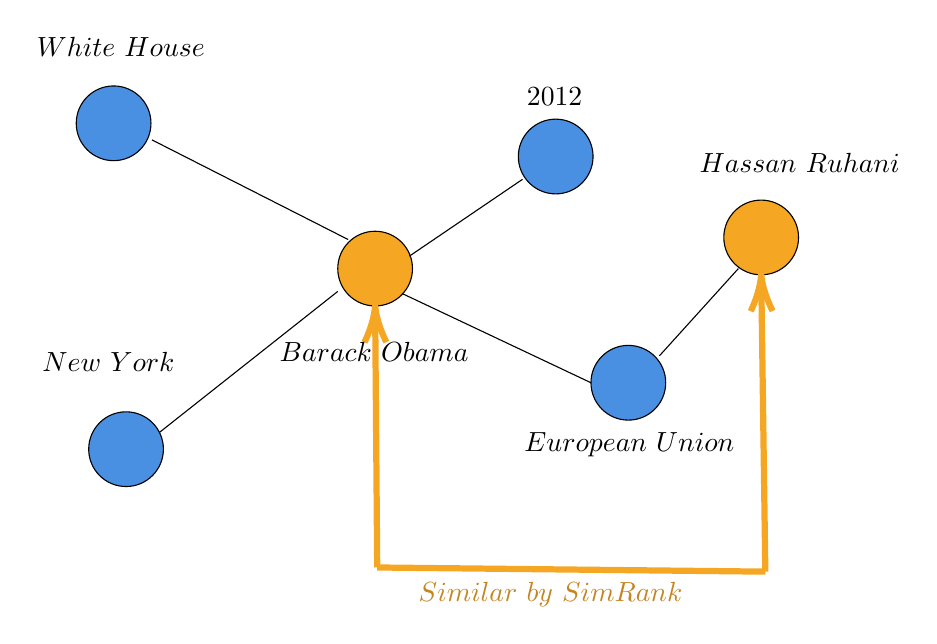
\begin{tikzpicture}[x=0.75pt,y=0.75pt,yscale=-1,xscale=1]
%uncomment if require: \path (0,407); %set diagram left start at 0, and has height of 407

%Shape: Circle [id:dp7237033228697587] 
\draw  [color={rgb, 255:red, 0; green, 0; blue, 0 }  ,draw opacity=1 ][fill={rgb, 255:red, 74; green, 144; blue, 226 }  ,fill opacity=1 ] (142.5,97) .. controls (142.5,87.06) and (150.56,79) .. (160.5,79) .. controls (170.44,79) and (178.5,87.06) .. (178.5,97) .. controls (178.5,106.94) and (170.44,115) .. (160.5,115) .. controls (150.56,115) and (142.5,106.94) .. (142.5,97) -- cycle ;
%Straight Lines [id:da7651994649420626] 
\draw    (179,105) -- (273.5,153) ;


%Shape: Circle [id:dp1628508691866306] 
\draw  [color={rgb, 255:red, 0; green, 0; blue, 0 }  ,draw opacity=1 ][fill={rgb, 255:red, 74; green, 144; blue, 226 }  ,fill opacity=1 ] (148.5,254) .. controls (148.5,244.06) and (156.56,236) .. (166.5,236) .. controls (176.44,236) and (184.5,244.06) .. (184.5,254) .. controls (184.5,263.94) and (176.44,272) .. (166.5,272) .. controls (156.56,272) and (148.5,263.94) .. (148.5,254) -- cycle ;
%Shape: Circle [id:dp6369036191517297] 
\draw  [color={rgb, 255:red, 0; green, 0; blue, 0 }  ,draw opacity=1 ][fill={rgb, 255:red, 245; green, 166; blue, 35 }  ,fill opacity=1 ] (268.5,167) .. controls (268.5,157.06) and (276.56,149) .. (286.5,149) .. controls (296.44,149) and (304.5,157.06) .. (304.5,167) .. controls (304.5,176.94) and (296.44,185) .. (286.5,185) .. controls (276.56,185) and (268.5,176.94) .. (268.5,167) -- cycle ;
%Shape: Circle [id:dp6138711151460285] 
\draw  [color={rgb, 255:red, 0; green, 0; blue, 0 }  ,draw opacity=1 ][fill={rgb, 255:red, 74; green, 144; blue, 226 }  ,fill opacity=1 ] (390.5,222) .. controls (390.5,212.06) and (398.56,204) .. (408.5,204) .. controls (418.44,204) and (426.5,212.06) .. (426.5,222) .. controls (426.5,231.94) and (418.44,240) .. (408.5,240) .. controls (398.56,240) and (390.5,231.94) .. (390.5,222) -- cycle ;
%Shape: Circle [id:dp15908024717263558] 
\draw  [color={rgb, 255:red, 0; green, 0; blue, 0 }  ,draw opacity=1 ][fill={rgb, 255:red, 74; green, 144; blue, 226 }  ,fill opacity=1 ] (355.5,113) .. controls (355.5,103.06) and (363.56,95) .. (373.5,95) .. controls (383.44,95) and (391.5,103.06) .. (391.5,113) .. controls (391.5,122.94) and (383.44,131) .. (373.5,131) .. controls (363.56,131) and (355.5,122.94) .. (355.5,113) -- cycle ;
%Straight Lines [id:da4548959711882159] 
\draw    (303,161) -- (357.5,124) ;


%Straight Lines [id:da6860631222603604] 
\draw    (299.5,179) -- (390.5,222) ;


%Straight Lines [id:da5778462671903315] 
\draw    (423.5,209) -- (461.5,167) ;


%Shape: Circle [id:dp9805133554604324] 
\draw  [color={rgb, 255:red, 0; green, 0; blue, 0 }  ,draw opacity=1 ][fill={rgb, 255:red, 245; green, 166; blue, 35 }  ,fill opacity=1 ] (454.5,152) .. controls (454.5,142.06) and (462.56,134) .. (472.5,134) .. controls (482.44,134) and (490.5,142.06) .. (490.5,152) .. controls (490.5,161.94) and (482.44,170) .. (472.5,170) .. controls (462.56,170) and (454.5,161.94) .. (454.5,152) -- cycle ;
%Straight Lines [id:da3078528737086299] 
\draw    (182.5,246) -- (268.5,178) ;


%Straight Lines [id:da6689641936732076] 
\draw [color={rgb, 255:red, 245; green, 166; blue, 35 }  ,draw opacity=1 ][line width=2.25]    (287.5,311) -- (286.53,189) ;
\draw [shift={(286.5,185)}, rotate = 449.55] [color={rgb, 255:red, 245; green, 166; blue, 35 }  ,draw opacity=1 ][line width=2.25]    (17.49,-5.26) .. controls (11.12,-2.23) and (5.29,-0.48) .. (0,0) .. controls (5.29,0.48) and (11.12,2.23) .. (17.49,5.26)   ;

%Straight Lines [id:da23704536821016675] 
\draw [color={rgb, 255:red, 245; green, 166; blue, 35 }  ,draw opacity=1 ][line width=2.25]    (474.5,313) -- (472.56,174) ;
\draw [shift={(472.5,170)}, rotate = 449.2] [color={rgb, 255:red, 245; green, 166; blue, 35 }  ,draw opacity=1 ][line width=2.25]    (17.49,-5.26) .. controls (11.12,-2.23) and (5.29,-0.48) .. (0,0) .. controls (5.29,0.48) and (11.12,2.23) .. (17.49,5.26)   ;

%Straight Lines [id:da7509045062366104] 
\draw [color={rgb, 255:red, 245; green, 166; blue, 35 }  ,draw opacity=1 ][line width=2.25]    (287.5,311) -- (474.5,313) ;



% Text Node
\draw (164,60) node   {$White\ House$};
% Text Node
\draw (286,207) node   {$Barack\ Obama$};
% Text Node
\draw (409,252) node   {$European\ Union$};
% Text Node
\draw (491,116) node   {$Hassan\ Ruhani$};
% Text Node
\draw (158,212) node   {$New\ York$};
% Text Node
\draw (373,84) node   {$2012$};
% Text Node
\draw (371,324) node [color={rgb, 255:red, 196; green, 133; blue, 33 }  ,opacity=1 ]  {$Similar\ by\ SimRank$};


\end{tikzpicture}


}
\caption{An example of SimRank similarity. In this graph, although the relationship between the president of Iran and the US is discovered by SimRank, the more important relationships, namely direct neighbours are disregarded. The similarity between \emph{``Barack Obama''} and the direct neighbours are zero.}
\label{fig:simrank}
\end{figure}
\noindent
% BR: This requires some details or back-references if you already
% talked about the model. How is the Adjacency Similarity defined, for
% example?
The VERSE model does not support the incorporation of the edge weights. From the three similarity measures that VERSE offers, we chose Adjacency Similarity, explained in Chapter~\ref{chap:background} in Section~\ref{subsec:VERSE}, to produce the entity embeddings. Our reason is two-fold: first, the PPR, explained in Chapter~\ref{chap:background} in Section~\ref{subsec:VERSE}, relates to the stationary distribution of a random walk with restart and we already represented the random walk-based models with DeepWalk.
% BR: Where does the PPR drop from? Give a quick refresher here and
% refer to the appropriate section in your document.
Second, SimRank, explained in Chapter~\ref{chap:background} in Section~\ref{subsec:VERSE}, is a measure of structural relatedness, between two nodes, based on the assumption that two nodes are similar if they are connected to other similar nodes. Although words that co-occur often with the same words can themselves be considered similar, if we only look at nodes that have common neighbours we lose most of the adjacency relations in the graph. An example is illustrated in Figure~\ref{fig:simrank}. Since the SimRank of two nodes with no common neighbour is zero, the direct neighbours are disregarded. However, SimRank tends to discover interesting relationships, such as the one shown in Figure~\ref{fig:simrank} and possibly if a new similarity measure is introduced that creates a trade-off between SimRank and Adjacency Similarity, the results might improve. For this study, however, we choose only Adjacency Similarity to learn the embeddings and we leave the development of a new similarity measure as future work. 
% BR: ...and we leave the development of a new similarity measure as
% future work
Since Adjacency Similarity is based on the normalized adjacency matrix, it captures the neighbourhood relations.
% BR: Rephrase: Since it [i.e. Adjacency Similarity] is based on the
% normalized adjacency matrix, ...
We could not use the LINE model for the following reasons : First, because of the unbalanced weight distribution, the optimization objective for the second-order proximity of the LINE model becomes ill-defined. Hence, one part of the embedding for this model cannot be trained properly. Second, the Adjacency Similarity of VERSE model correlates with the first-order proximity in LINE and can be used as representative of first-order proximity.  \\
% BR: Same issue: SimRank appears to drop out of nowhere and needs to be
% put into context.
\section{Summary}\label{sec:entity_summary}
In this chapter, two methods to extract entity and term embeddings from an annotated corpus were introduced. One method learns the embeddings directly from the text, while the other one generates a co-occurrence graph and embeds the nodes. In the next chapter we attempt to create embeddings separable by entity type and in in Chapter~\ref{chap:eval}, we report the evaluation results for both entity based and faceted embeddings. We also show why the extraction of a co-occurrence graph is crucial for achieving better performance. 
% BR: If you developed this by yourself, you can give yourself more
% credit :-]
